\subsection{Bài tập trắc nghiệm}
\subsubsection{Câu hỏi trắc nghiệm 4 phương án}
\begin{dang}{Nhận biết tỉ số lượng giác của góc nhọn. Tính tỉ số lượng giác của góc nhọn trong tam giác vuông}
\end{dang}
\Opensolutionfile{ans}[ans/ans-9-B16-TN-D1]
%%==========Câu 1
\begin{ex}%[9H4N1-1]
	%
	\immini[thm]
	{
	Trong hình vẽ sau, $\sin B$ bằng
	\choice
	{$\dfrac{AB}{BC}$}
	{\True $\dfrac{AC}{BC}$}
	{$\dfrac{AC}{AB}$}
	{$\dfrac{AB}{AC}$}
	}
	{
	\begin{tikzpicture}[>=stealth,line join=round,line cap=round,font=\footnotesize,scale=.7]
	\path
	(0,0) coordinate (A)
	(90:3) coordinate (B)
	(0:2) coordinate (C)
	;
	\draw (A)--(B)--(C)--cycle;
	\draw pic[draw,angle radius=2mm] {right angle = C--A--B};
	\foreach \d/\g in{A/200,B/90,C/-20} \fill[] (\d) circle (1.2pt) node at ($(\d)+(\g:3mm)$){$\d$};
	\end{tikzpicture}
	}
	\loigiai{
	Xét tam giác $ABC$ vuông tại $A$ có $\sin B=\dfrac{AC}{BC}$}
\end{ex}
%%==========Câu 2
\begin{ex}%[9H4N1-1]
	%
	\immini[thm]
	{
	Trong hình vẽ sau, $\cos B$ bằng
	\choice
	{\True $\dfrac{BH}{AB}$}
	{$\dfrac{AH}{AB}$}
	{$\dfrac{BH}{AH}$}
	{$\dfrac{AB}{AC}$}
	}
	{
	\begin{tikzpicture}[>=stealth,line join=round,line cap=round,font=\footnotesize,scale=.7]
	\path
	(0,0)coordinate (B)
	(60:.2)coordinate (B1)
	(0:4) coordinate (C)
	($(C)+(150:.1)$)coordinate (C1)
	(intersection of B--B1 and C--C1) coordinate (A)
	($(B)!(A)!(C)$) coordinate (H)
	;
	\draw (A)--(B)--(C)--cycle (A)--(H);
	\foreach \d/\g in{A/90,B/200,C/-20,H/-90} \fill[] (\d) circle (1.2pt) node at ($(\d)+(\g:3mm)$){$\d$};
	\draw pic[draw,angle radius=2mm] {right angle = B--A--C};
	\draw pic[draw,angle radius=2mm] {right angle = C--H--A};
	\end{tikzpicture}
	}
	\loigiai{
	Xét tam giác $ABC$ vuông tại $A$ có $\cos B=\dfrac{BH}{AB}$}
\end{ex}
%%==========Câu 3
\begin{ex}%[9H4N1-1]
	%
	\immini[thm]
	{
	Trong hình vẽ sau, $\tan C$ bằng
	\choice
	{$\dfrac{BH}{AB}$}
	{$\dfrac{AH}{AB}$}
	{$\dfrac{BH}{AH}$}
	{\True $\dfrac{AB}{AC}$}
	}
	{
	\begin{tikzpicture}[>=stealth,line join=round,line cap=round,font=\footnotesize,scale=.7]
	\path
	(0,0)coordinate (B)
	(60:.2)coordinate (B1)
	(0:4) coordinate (C)
	($(C)+(150:.1)$)coordinate (C1)
	(intersection of B--B1 and C--C1) coordinate (A)
	($(B)!(A)!(C)$) coordinate (H)
	;
	\draw (A)--(B)--(C)--cycle (A)--(H);
	\foreach \d/\g in{A/90,B/200,C/-20,H/-90} \fill[] (\d) circle (1.2pt) node at ($(\d)+(\g:3mm)$){$\d$};
	\draw pic[draw,angle radius=2mm] {right angle = B--A--C};
	\draw pic[draw,angle radius=2mm] {right angle = C--H--A};
	\end{tikzpicture}
	}
	\loigiai{
	Xét tam giác $ABC$ vuông tại $A$ có $\tan C=\dfrac{AB}{AC}$}
\end{ex}
%%==========Câu 4
\begin{ex}%[9H4N1-1]
	%
	$\cot 30^\circ$ bằng
	\choice
	{\True$\sqrt{3}$}
	{$\dfrac{1}{2}$}
	{$\dfrac{1}{3}$}
	{$\dfrac{\sqrt{3}}{3}$}
	\loigiai{
	$\cot 30^\circ=\sqrt{3}$}
\end{ex}
%%==========Câu 5
\begin{ex}%[9H4N1-1]
	%
	$\cos 46^\circ 28'$ (kết quả làm tròn đến chữ số thập phân thứ ba) bằng
	\choice
	{$0,723$}
	{\True $0,689$}
	{$0,950$}
	{$0,691$}
	\loigiai{
	$\cos 46^\circ 28'\approx 0,689$}
\end{ex}
%%==========Câu 6
\begin{ex}%[9H4N1-1]
	%
	Nếu $\tan \alpha=1,123$ thì số đo góc $\alpha$ là (kết quả làm tròn đến phút)
	\choice
	{\True $48^\circ 19'$}
	{$48^\circ 18'$}
	{$48^\circ 32'$}
	{$48^\circ 31'$}
	\loigiai{
	Vì $\tan \alpha=1,123$ nên $\alpha \approx 48^\circ 19'$}
\end{ex}
%%==========Câu 7
\begin{ex}%[9H4N1-1]
	%
	Cho tam giác $ABC$ vuông tại $A$, biết $AB=6\mathrm{~cm}$, $AC=8\mathrm{~cm}$. Khi đó $\tan B$ có giá trị là
	\choice
	{$\dfrac{6}{10}$}
	{\True $\dfrac{4}{3}$}
	{$\dfrac{3}{4}$}
	{$\dfrac{4}{5}$}
	\loigiai{
	Xét tam giác $ABC$ vuông tại $A$ có: $\tan B=\dfrac{AC}{AB}=\dfrac{8}{6}=\dfrac{4}{3}$}
\end{ex}
%%==========Câu 8
\begin{ex}%[9H4H1-1]
%
Cho tam giác $ABC$ vuông tại $A$, biết $AC=3\mathrm{~cm}$, $BC=5\mathrm{~cm}$. Khi đó $\sin B+\cos C$ có giá trị là
\choice
{\True $\dfrac{6}{5}$}
{$\dfrac{3}{5}$}
{$\dfrac{5}{6}$}
{$1$}
\loigiai{
Xét tam giác $ABC$ vuông tại $A$, Theo định lí Pythagore $BC^2=AB^2+AC^2$ \\
Mà $AC=3\mathrm{~cm}$, $BC=5\mathrm{~cm}$. Do đó $AB=4\mathrm{~cm}$.\\
Vậy $\sin B+\cos C=\dfrac{AC}{BC}+\dfrac{AC}{BC}=\dfrac{3}{5}+\dfrac{3}{5}=\dfrac{6}{5}$}
\end{ex}
%%==========Câu 9
\begin{ex}%[9H4N1-1]
	%
	Cho tam giác $ABC$ biết $AB=6\mathrm{~cm}$; $AC=8\mathrm{~cm}$; $BC=10\mathrm{~cm}$. Khi đó $\cot B$ có giá trị là
	\choice
	{$\dfrac{4}{3}$}
	{$\dfrac{3}{5}$}
	{\True $\dfrac{3}{4}$}
	{$\dfrac{4}{5}$}
	\loigiai{
	\begin{center}
	\begin{tikzpicture}[>=stealth,line join=round,line cap=round,font=\footnotesize,scale=1]
	\path
	(0,0) coordinate (A)
	(90:3) coordinate (B)
	(0:2) coordinate (C)
	;
	\draw (A)--(B)--(C)--cycle;
	\draw pic[draw,angle radius=2mm] {right angle = C--A--B};
	\foreach \d/\g in{A/200,B/90,C/-20} \fill[] (\d) circle (1.2pt) node at ($(\d)+(\g:3mm)$){$\d$};
	\end{tikzpicture}
	\end{center}
	Ta có $AB=6\mathrm{~cm}$; $AC=8\mathrm{~cm}$; $BC=10\mathrm{~cm}$.\\
	Do đó $BC^2=AB^2+AC^2$. Theo định lí Pythagore đảo $\triangle ABC$ vuông tại $A$.\\
	Vậy $\cot B=\dfrac{AB}{AC}=\dfrac{6}{8}=\dfrac{3}{4}$}
\end{ex}
%%==========Câu 10
\begin{ex}%[9H4H1-1]
%
Cho tam giác $ABC$ vuông tại $A$, đường cao $AH$ $\left(H\in BC\right)$. Biết $HB=4\mathrm{~cm}$; $HC=12\mathrm{~cm}$. Khi đó $\tan B$ bằng
\choice
{\True $\sqrt{3}$}
{$\dfrac{4}{3}$}
{$\dfrac{\sqrt{3}}{3}$}
{$1$}
\loigiai{
\begin{center}
\begin{tikzpicture}[>=stealth,line join=round,line cap=round,font=\footnotesize,scale=1]
\path
(0,0)coordinate (B)
(60:.2)coordinate (B1)
(0:4) coordinate (C)
($(C)+(150:.1)$)coordinate (C1)
(intersection of B--B1 and C--C1) coordinate (A)
($(B)!(A)!(C)$) coordinate (H)
;
\draw (A)--(B)--(C)--cycle (A)--(H);
\foreach \d/\g in{A/90,B/200,C/-20,H/-90} \fill[] (\d) circle (1.2pt) node at ($(\d)+(\g:3mm)$){$\d$};
\draw pic[draw,angle radius=2mm] {right angle = B--A--C};
\draw pic[draw,angle radius=2mm] {right angle = C--H--A};
\end{tikzpicture}
\end{center}
Xét tam giác $ABC$ vuông tại $A$, đường cao $AH$ $\left(H\in BC\right)$. Ta có $AH^2=HB.HC=4.12=48$ \\
Suy ra $AH=\sqrt{48}=4\sqrt{3}\mathrm{~cm}$ \\
Xét tam giác $AHB$ vuông tại $H$, ta có: $\tan B=\dfrac{AH}{HB}=\dfrac{4\sqrt{3}}{4}=\sqrt{3}$}
\end{ex}
\Closesolutionfile{ans}
\indapan{10}{ans/ans-9-B16-TN-D1}
\begin{dang}{ Nhận biết 2 góc phụ nhau. Sử dụng tỉ số lượng giác của hai góc phụ nhau so sánh, sắp xếp các tỉ số lượng giác}
\end{dang}
\Opensolutionfile{ans}[ans/ans-9-B16-TN-D2]
%%==========Câu 11
\begin{ex}%[9H4N1-2]
%
Hệ thức nào sau đây \textbf{sai}?
\choice
{$\sin 38^\circ=\cos \text{52}^\circ$}
{$\cos \text{42}^\circ=\sin 48^\circ$}
{$\tan 50^\circ=\cot 40^\circ$}
{\True $\cot 20^\circ=\tan 80^\circ$}
\loigiai{
Hệ thức sai là $\cot 20^\circ=\tan 80^\circ$}
\end{ex}
%%==========Câu 12
\begin{ex}%[9H4N1-6]
	%
	Cho $\alpha+\beta=90^\circ$, ta có
	\choice
	{$\sin \alpha=\sin \beta$}
	{$\sin \alpha=c\mathrm{os}\alpha$}
	{$\tan \alpha=\tan \beta$}
	{\True $\tan \alpha=\cot \beta$}
	\loigiai{
	Cho $\alpha+\beta=90^\circ$, ta có $\tan \alpha=\cot \beta$}
\end{ex}
%%==========Câu 13
\begin{ex}%[9H4N1-6]
	%
	Cho $\alpha+\beta=90^\circ$. Hệ thức nào sau đây không đúng?
	\choice
	{$\sin \alpha=\cos \left(90^\circ-\alpha\right)$}
	{$\cos \alpha=\sin \beta$}
	{\True $\tan \alpha=\cot \left(90^\circ-\beta\right)$}
	{$\cot \alpha=\tan \left(90^\circ-\alpha\right)$}
	\loigiai{
	Hệ thức không đúng là $\tan \alpha=\cot \left(90^\circ-\beta\right)$}
\end{ex}
%%==========Câu 14
\begin{ex}%[9H4N1-6]
	%
	Cho hai góc nhọn $\alpha$, $\beta$ Biết $\alpha < \beta$, hệ thức nào sau đây không đúng?
	\choice
	{$\sin \alpha < \sin \beta$}
	{$\cos \alpha > \cos \beta$}
	{\True $\cot \alpha < \cot \beta$}
	{$\tan \alpha < \tan \beta$}
	\loigiai{
	Hệ thức không đúng là $\cot \alpha < \cot \beta$}
\end{ex}
%%==========Câu 15
\begin{ex}%[9H4H1-2]
	%
	Giá trị của biểu thức $\dfrac{\tan 47^\circ}{\cot 43^\circ}$ bằng
	\choice
	{\True $1$}
	{$0$}
	{$2\tan 47^\circ$}
	{$2\cot 43^\circ$}
	\loigiai{
	Vì $\cot 43^\circ=\tan 47^\circ$ nên $\dfrac{\tan 47^\circ}{\cot 43^\circ}=\dfrac{\tan 47^\circ}{\tan 47^\circ}=1$}
\end{ex}
%%==========Câu 16
\begin{ex}%[9H4H1-2]
	%
	Trong các khẳng định sau, khẳng định nào đúng?
	\choice
	{$\sin 36^\circ=\cot 54^\circ$}
	{$\tan 36^\circ=\cos 54^\circ$}
	{$\cot 36^\circ=\dfrac{1}{\tan^236^\circ}$}
	{\True $\tan 36^\circ=\dfrac{1}{\cot 36^\circ}$}
	\loigiai{
	Trong các khẳng định, khẳng định đúng là $\tan 36^\circ=\dfrac{1}{\cot 36^\circ}$}
\end{ex}
%%==========Câu 17
\begin{ex}%[9H4H1-2]
	%
	Giá trị của biểu thức $\sin 48^\circ-\cos 42^\circ$ bằng
	\choice
	{$1$}
	{\True $0$}
	{$2\tan 47^\circ$}
	{$2\cot 43^\circ$}
	\loigiai{
	Giá trị của biểu thức $\sin 48^\circ-\cos 42^\circ=\sin 48^\circ-\sin 48^\circ=0$.}
\end{ex}
%%==========Câu 18
\begin{ex}%[9H4H1-2]
	%
	Sắp xếp các tỉ số lượng giác $\sin 34^\circ$; $\cos 55^\circ$; $\sin 28^\circ$; $\cos 63^\circ$ theo thứ tự tăng dần ta được kết quả là
	\choice
	{\True $\cos 63^\circ < \sin 28^\circ < \sin 34^\circ < \cos 55^\circ$}
	{$\sin 28^\circ < \sin 34^\circ < \cos 55^\circ < \cos 63^\circ$}
	{$\cos 55^\circ < \sin 34^\circ < \sin 28^\circ < \cos 63^\circ$}
	{$\cos 55^\circ < \cos 63^\circ < \sin 28^\circ < \sin 34^\circ$}
	\loigiai{
	Ta có $\cos 63^\circ=\sin 27^\circ$; $\cos 55^\circ=\sin 35^\circ$ \\
	Vì $\sin 27^\circ < \sin 28^\circ < \sin 34^\circ < \sin 35^\circ$ nên $\cos 63^\circ < \sin 28^\circ < \sin 34^\circ < \cos 55^\circ$.}
\end{ex}
%%==========Câu 19
\begin{ex}%[9H4H1-2]
	%
	Sắp xếp các tỉ số lượng giác $\tan 34^\circ$; $\tan 55^\circ$; $\cot 28^\circ$; $\cot 63^\circ$ theo thứ tự tăng dần ta được kết quả là
	\choice
	{\True $\cot 63^\circ < \tan 34^\circ < \tan 55^\circ < \cot 28^\circ$}
	{$\tan 34^\circ < \cot 28^\circ < \cot 63^\circ < \tan 55^\circ$}
	{$\cot 28^\circ < \cot 63^\circ < \tan 55^\circ < \tan 34^\circ$}
	{$\tan 55^\circ < \tan 34^\circ < \cot 28^\circ < \cot 63^\circ$}
	\loigiai{
	Ta có $\cot 28^\circ=\tan 62^\circ$; $\cot 63^\circ=\tan 27^\circ$ \\
	Vỉ $\tan 27^\circ < \tan 34^\circ < \tan 55^\circ < \tan 62^\circ$ nên $\cot 63^\circ < \tan 34^\circ < \tan 55^\circ < \cot 28^\circ$.}
\end{ex}
%%==========Câu 20
\begin{ex}%[9H4C1-2]
%
Giá trị biểu thức $A=\tan 1^\circ.\tan 2^\circ.\tan 3^\circ..\tan 89^\circ$ bằng
\choice
{$0$}
{\True $1$}
{$\sqrt{2}$}
{$2\cot 45^\circ$}
\loigiai{
$A=\tan 1^\circ.\tan 2^\circ.\tan 3^\circ..\tan 89^\circ$ \\
$A=\tan 1^\circ.\tan 2^\circ.\tan 3^\circ..\tan 87^\circ.\tan 88^\circ.\tan 89^\circ$ \\
$A=\tan 1^\circ.\tan 2^\circ.\tan 3^\circ..\cot 1^\circ.\cot 2^\circ.\cot 3^\circ$ \\
$A=\left(\tan 1^\circ.\cot 1^\circ\right).\left(\tan 2^\circ.\cot 2^\circ\right).\left(\tan 3^\circ.\cot 3^\circ\right)..\cot 45^\circ$ \\
$A=1.1.1..1=1$}
\end{ex}
\Closesolutionfile{ans}
\indapan{10}{ans/ans-9-B16-TN-D2}
\begin{dang}{Tính góc, cạnh trong tam giác vuông}
\end{dang}
\Opensolutionfile{ans}[ans/ans-9-B16-TN-D3]
%%==========Câu 21
\begin{ex}%[9H4H1-3]
	%
	Cho tam giác $ABC$ vuông tại $A$, biết $\tan B=\dfrac{2}{3}$, $AB=6\mathrm{~cm}$. Độ dài cạnh $AC$ là
	\choice
	{$3\mathrm{~cm}$}
	{\True $4\mathrm{~cm}$}
	{$9\mathrm{~cm}$}
	{$16\mathrm{~cm}$}
	\loigiai{
	Xét tam giác $ABC$ vuông tại $A$, có $\tan B=\dfrac{AC}{AB}$ suy ra $AC=AB.\tan B$ hay $AC=6\cdot \dfrac{2}{3}=4\mathrm{~cm}$}
\end{ex}
%%==========Câu 22
\begin{ex}%[9H4H1-3]
	%
	Cho tam giác $ABC$ vuông tại $A$, biết $\sin B=\dfrac{2}{3}$, $BC=6\mathrm{~cm}$. Độ dài cạnh $AC$ là
	\choice
	{$3\mathrm{~cm}$}
	{\True $4\mathrm{~cm}$}
	{$9\mathrm{~cm}$}
	{$16\mathrm{~cm}$}
	\loigiai{
	Xét tam giác $ABC$ vuông tại $A$, có $\sin B=\dfrac{AC}{BC}$ suy ra $AC=BC.\sin B$ suy ra $AC=6\cdot \dfrac{2}{3}=4\mathrm{~cm}$}
\end{ex}
%%==========Câu 23
\begin{ex}%[9H4H1-3]
	%
	Cho tam giác $MNP$ vuông tại $M$, biết $\cot N=\dfrac{1}{3}$, $MP=9\mathrm{~cm}$. Độ dài cạnh $MN$ là
	\choice
	{\True $3\mathrm{~cm}$}
	{$4\mathrm{~cm}$}
	{$9\mathrm{~cm}$}
	{$16\mathrm{~cm}$}
	\loigiai{
	Xét tam giác $MNP$ vuông tại $M$ ta có $\cot N=\dfrac{MN}{MP}$ suy ra $MN=MP.\cot N$ hay $MN=9\cdot \dfrac{1}{3}=3\mathrm{~cm}$}
\end{ex}
%%==========Câu 24
\begin{ex}%[9H4H1-3]
	%
	Cho tam giác $IHK$ vuông tại $H$, biết $\cos K=\dfrac{3}{4}$, $IK=12\mathrm{~cm}$. Độ dài cạnh $HK$ là
	\choice
	{$3\mathrm{~cm}$}
	{$4\mathrm{~cm}$}
	{\True $9\mathrm{~cm}$}
	{$16\mathrm{~cm}$}
	\loigiai{
	Xét tam giác $IHK$ vuông tại $H$ ta có $\cos K=\dfrac{KH}{IK}$ suy ra $KH=IK.\cos K$ hay $KH=12\cdot \dfrac{3}{4}=9\mathrm{~cm}$}
\end{ex}
%%==========Câu 25
\begin{ex}%[9H4H1-3]
	%
	Cho tam giác $ABC$ vuông tại $A$, biết $\widehat{B}=30^\circ$, $BC=2\mathrm{~cm}$. Độ dài cạnh $AB$ là
	\choice
	{\True $\sqrt{3}$}
	{$2\sqrt{3}$}
	{$\dfrac{1}{\sqrt{3}}$}
	{$\dfrac{2}{\sqrt{3}}$}
	\loigiai{
	Xét tam giác $ABC$ vuông tại $A$, có $\cos B=\dfrac{AB}{BC}$ \\
	$AB=BC.\cos B$ \\
	$AB=2.\cos 30^\circ=\sqrt{3}\mathrm{~cm}$}
\end{ex}
%%==========Câu 26
\begin{ex}%[9H4H1-3]
	%
	Cho tam giác $ABC$ vuông tại $A$, biết $\widehat{C}=45^\circ$, $BC=5\mathrm{~cm}$. Độ dài cạnh $AC$ là
	\choice
	{\True $\dfrac{5\sqrt{2}}{2}\mathrm{~cm}$}
	{$5\sqrt{2}\mathrm{~cm}$}
	{$\dfrac{5}{2}\mathrm{~cm}$}
	{$\dfrac{5}{\sqrt{5}}\mathrm{~cm}$}
	\loigiai{
	Xét tam giác $ABC$ vuông tại $A$, có $\cos C=\dfrac{AC}{BC}$ \\
	$AC=BC.\cos C$ \\
	$AC=5.\cos 45^\circ=\dfrac{5\sqrt{2}}{2}\mathrm{~cm}$}
\end{ex}
%%==========Câu 27
\begin{ex}%[9H4H1-3]
	%
	Cho tam giác $MNP$ vuông tại $M$, có $MN=3\mathrm{~cm}$, $NP=5\mathrm{~cm}$. Số đo góc $N$ (làm tròn đến độ) là
	\choice
	{\True $53^\circ$}
	{$37^\circ$}
	{$31^\circ$}
	{$59^\circ$}
	\loigiai{
	Xét tam giác $MNP$ vuông tại $M$, ta có: $\cos N=\dfrac{MN}{NP}=\dfrac{3}{5}$ suy ra $\widehat{N}\approx 53^\circ$.}
\end{ex}
%%==========Câu 28
\begin{ex}%[9H4H1-5]
%
\immini[thm]
{
Khi tia nắng mặt trời tạo với mặt đất một góc $72^\circ$ thì bóng của một tòa nhà cao tầng trên mặt đất dài $36~m$ (hình vẽ). Chiều cao của toàn nhà (làm tròn đến hàng đơn vị) là
\choice
{\True $111m$}
{$112m$}
{$110m$}
{$113m$}
}
{
%!<\usepackage{amsmath,amssymb}>
%!<\usetikzlibrary{calc}>
\begin{tikzpicture}[line cap=round, line join=round, thick, scale=0.6,transform shape]
	% --- Bắt đầu mã ngôi nhà từ file đính kèm (Hình H1) ---
	\def\a{1.4}
	\def\xd{-0.4}
	\def\dy{0.3}
	\def\h{6}
	% Các mặt của tòa nhà
	\fill[gray!15] (-\a,0) rectangle (0,\h);
	\fill[gray!25] (-\a,0) -- (-\a+\xd, \dy) -- (-\a+\xd, \h+\dy) -- (-\a, \h) -- cycle;
	\fill[gray!5] (-\a, \h) -- (-\a+\xd, \h+\dy) -- (\xd, \h+\dy) -- (0, \h) -- cycle;
	% Các đường viền tòa nhà
	\draw[gray!40, line width=0.6pt] (-\a,0) rectangle (0,\h);
	\draw[gray!40, line width=0.6pt] (-\a,0) -- (-\a+\xd, \dy) -- (-\a+\xd, \h+\dy) -- (-\a, \h);
	\draw[gray!40, line width=0.6pt] (-\a+\xd, \h+\dy) -- (\xd, \h+\dy) -- (0, \h);
	% Các cửa sổ
	\foreach \y in {0.4, 1.0, 1.6, 2.2, 3.4, 4.0, 4.6, 5.2} {
	\fill[cyan!30, draw=black!40, line width=0.6pt] (-\a+0.15, \y) rectangle (-0.15, \y+0.4);
	\fill[cyan!30, draw=black!40, line width=0.6pt] (-\a+\xd+0.1, \y+\dy+0.05) -- (-\a-0.05, \y+0.05) -- (-\a-0.05, \y+0.35) -- (-\a+\xd+0.1, \y+\dy+0.35) -- cycle;
	}
	% Tầng có màu cam
	\fill[orange!30, draw=black!40, line width=0.6pt] (-\a+0.15, 2.8) rectangle (-0.15, 2.8+0.4);
	\fill[orange!30, draw=black!40, line width=0.6pt] (-\a+\xd+0.1, 2.8+\dy+0.05) -- (-\a-0.05, 2.8+0.05) -- (-\a-0.05, 2.8+0.35) -- (-\a+\xd+0.1, 2.8+\dy+0.35) -- cycle;
	% --- Kết thúc mã ngôi nhà ---
	% Định nghĩa các điểm của tam giác ABC
	\coordinate (A) at (0,0);
	\coordinate (B) at (0,\h);
	% tan(72 độ) xấp xỉ 3.07 -> AC = AB / 3.07 = 6 / 3.07 = 1.95
	\coordinate (C) at (1.95,0);
	% Vẽ mặt đất
	\draw (-2.5,0) -- (3,0);
	% Vẽ mô hình tam giác
	\draw[ultra thick] (A) -- (B) -- (C) -- cycle;
	% Ký hiệu góc vuông tại A
	\draw[thick] (0,0.25) -- (0.25,0.25) -- (0.25,0);
	% Nhãn các đỉnh
	\node[below, font=\bfseries] at (A) {$A$};
	\node[above, font=\bfseries] at (B) {$B$};
	\node[below right, font=\bfseries] at (C) {$C$};
	% Nhãn độ dài và góc
	\node[below] at ($(A)!0.5!(C)$) {$36 \, m$};
	\draw (C) ++(-0.5,0) arc (180:108:0.5);
	\node[font=\footnotesize] at ($(C)+(-0.7,0.3)$) {$72^\circ$};
\end{tikzpicture}
}
\loigiai{
Gọi chiều cao toà nhà là $AB$, góc tạo bởi tia nắng mặt trời và mặt đất là $\widehat{C}=72^\circ$, bóng toà nhà dưới mặt đất là $AC=36m$.\\
Xét tam giác $ABC$ vuông tại $A$, Ta có $\tan C=\dfrac{AB}{AC}$ \\
$AB=AC.\tan C=36.\tan72^\circ\approx \text{111(m)}$ \\
Chiều cao của toàn nhà là $\text{111(m)}$}
\end{ex}
%%==========Câu 29
\begin{ex}%[9H4H1-3]
%
Tại một thời điểm trong ngày, một cột bê tông thẳng đứng bên đường cao $5m$ có bóng in trên mặt đất là $AC$ dài $3,2~m$. Số đo góc tạo bởi tia nắng mặt trời tạo với mặt đất thời điểm đó là
\choice
{\True $57^\circ23'$}
{$32^\circ62'$}
{$57^\circ22'$}
{$32^\circ37'$}
\loigiai{
Ta có góc tạo bởi tia nắng mặt trời và mặt đất là $\widehat{C}$.\\
Xét tam giác $ABC$ vuông tại $A$, ta có: $\tan C=\dfrac{AB}{AC}=\dfrac{5}{3,2}$ \\
$\widehat{C}\approx{57^\circ}23'$}
\end{ex}
%%==========Câu 30
\begin{ex}%[9H4V1-5]
%
\immini[thm]
{
Hai bạn học sinh Nam và Trung đang đứng ở mặt đất bằng phẳng, cách nhau 100m thì nhìn thấy một chiếc diều (ở khoảng giữa hai bạn). Biết góc \lq\lq nâng\rq\rq để nhìn thấy diều ở vị trí của Trung là $65^\circ$ và góc \lq\lq nâng\rq\rq để nhìn thấy diều ở vị trí của Nam là $30^\circ$ và khoảng cách từ mắt mỗi bạn đến mặt đất đều bằng ${1,62m}$. Độ cao của diều lúc đó so với mặt đất là (Kết quả làm tròn đến chữ số thập phân thứ hai).
\choice
{\True ${47,11m}$}
{${47,10m}$}
{${47,50m}$}
{${45,45m}$}
}
{
%!<\usetikzlibrary{calc,angles,quotes}>
\begin{tikzpicture}[
	declare function={a=0.5; b=0.3; d=0.8; goc=-50;},
	every node/.style={font=\normalsize},
	line join=round,
	ribbon/.style n args={2}{
	draw=#1, 
	line width=1pt, 
	preaction={draw=white, line width=1.8pt}, 
	postaction={draw=#2, line width=0.3pt}
	},scale=0.7,transform shape
	]
	% Define colors
	\definecolor{kiteY}{RGB}{244,192,89}
	\definecolor{kiteT}{RGB}{94,176,165}
	\definecolor{kiteB}{RGB}{17,130,182}
	\definecolor{kiteR}{RGB}{229,72,65}
	\definecolor{kiteBrown}{RGB}{160,82,45}
	% Define coordinates for the problem
	\coordinate (M) at (0,0);
	\coordinate (N) at (8,0);
	\coordinate (A) at (0,1.62);
	\coordinate (C) at (8,1.62);
	% Calculate point B (kite position)
	% AH + HC = 8
	% AH = BH * cot(65)
	% HC = BH * cot(30)
	% BH * (cot(65) + cot(30)) = 8 => BH = 8 / (cot(65) + cot(30))
	\pgfmathsetmacro{\bh}{8 / (cot(65) + cot(30))}
	\pgfmathsetmacro{\ah}{\bh * cot(65)}
	\coordinate (H) at (\ah, 1.62);
	\coordinate (B_kite) at (\ah, 1.62 + \bh);
	\coordinate (P) at (\ah, 0);
	% Draw lines for the problem
	\draw (M) -- (N);
	\draw (A) -- (C);
	\draw (A) -- (M) node[midway, left] {$1,62$ m};
	\draw (C) -- (N);
	\draw (A) -- (B_kite);
	\draw (C) -- (B_kite);
	\draw (B_kite) -- (P);
	% Draw right angle
	\draw (H) ++(-0.2,0) -- ++(0,0.2) -- ++(0.2,0);
	% Draw angles
	\pic[draw, angle radius=0.6cm, "$65^\circ$", angle eccentricity=1.5] {angle = C--A--B_kite};
	\pic[draw, angle radius=0.8cm, "$30^\circ$", angle eccentricity=1.5] {angle = B_kite--C--A};
	% Labels
	\node[below left] at (A) {$A$};
	\node[below right] at (C) {$C$};
	\node[below left] at (M) {$M$};
	\node[below right] at (N) {$N$};
	\node[below left] at (H) {$H$};
	\node[below right] at (P) {$P$};
	\node[above left] at (B_kite) {$B$};
	% Mark points
	\foreach \p in {A, C, M, N, H, P, B_kite} {
	\fill (\p) circle (1.5pt);
	}
	% --- Draw the kite at position B_kite ---
	\begin{scope}[shift={(B_kite)}]
	\path
	(0,0) coordinate (O)
	(goc:d) coordinate (D)
	(goc+180:b) coordinate (B)
	(goc+90:a) coordinate (C)
	(goc-90:a) coordinate (A)
	;
	\fill[kiteY] (O) -- (A) -- (B) -- cycle;
	\fill[kiteT] (O) -- (B) -- (C) -- cycle;
	\fill[kiteB] (O) -- (C) -- (D) -- cycle;
	\fill[kiteR] (O) -- (D) -- (A) -- cycle;
	\draw[white, line width=0.5pt] (A) -- (C);
	\draw[white, line width=0.5pt] (B) -- (D);
	\draw[white, line width=0.3pt] ($(A)!0.3!(B)!0.15!(O)$) -- ($(A)!0.3!(B)!0.45!(O)$);
	\draw[white, line width=0.3pt] ($(A)!0.45!(B)!0.15!(O)$) -- ($(A)!0.45!(B)!0.55!(O)$);
	\draw[white, line width=0.3pt] ($(A)!0.6!(B)!0.15!(O)$) -- ($(A)!0.6!(B)!0.45!(O)$);
	\draw[white, line width=0.3pt] ($(B)!0.4!(C)!0.15!(O)$) -- ($(B)!0.4!(C)!0.45!(O)$);
	\draw[white, line width=0.3pt] ($(B)!0.6!(C)!0.15!(O)$) -- ($(B)!0.6!(C)!0.45!(O)$);
	\draw[white, line width=0.3pt] ($(C)!0.3!(D)!0.15!(O)$) -- ($(C)!0.3!(D)!0.45!(O)$);
	\draw[white, line width=0.3pt] ($(C)!0.45!(D)!0.15!(O)$) -- ($(C)!0.45!(D)!0.65!(O)$);
	\draw[white, line width=0.3pt] ($(C)!0.6!(D)!0.15!(O)$) -- ($(C)!0.6!(D)!0.45!(O)$);
	\draw[white, line width=0.3pt] ($(D)!0.4!(A)!0.15!(O)$) -- ($(D)!0.4!(A)!0.45!(O)$);
	\draw[white, line width=0.3pt] ($(D)!0.55!(A)!0.15!(O)$) -- ($(D)!0.55!(A)!0.65!(O)$);
	\draw[white, line width=0.3pt] ($(D)!0.7!(A)!0.15!(O)$) -- ($(D)!0.7!(A)!0.45!(O)$);
	\begin{scope}[shift={(D)}, rotate=goc, scale=0.3]
	\draw[ribbon={kiteB}{kiteB!50!white}] (0,0) .. controls (0.5, -0.4) and (1.0, -0.7) .. (1.5, 0);
	\draw[ribbon={kiteY}{kiteY!50!white}] (0,0) .. controls (0.5, 0.2) and (1.0, -0.5) .. (1.5, -0.3);
	\draw[ribbon={kiteR}{kiteR!50!white}] (0,0) .. controls (0.5, -0.2) and (1.0, 0.5) .. (1.5, 0.3);
	\draw[ribbon={kiteT}{kiteT!50!white}] (0,0) .. controls (0.5, 0.5) and (1.0, 0.8) .. (1.5, 0);
	\draw[ribbon={kiteT}{kiteT!50!white}] (1.5, 0) .. controls (2.0, -0.8) and (2.5, -1.2) .. (3.0, 0);
	\draw[ribbon={kiteR}{kiteR!50!white}] (1.5, 0.3) .. controls (2.0, 0.1) and (2.5, -0.9) .. (3.0, -0.3);
	\draw[ribbon={kiteY}{kiteY!50!white}] (1.5, -0.3) .. controls (2.0, -0.1) and (2.5, 0.9) .. (3.0, 0.3);
	\draw[ribbon={kiteB}{kiteB!50!white}] (1.5, 0) .. controls (2.0, 0.7) and (2.5, 1.1) .. (3.0, 0);
	\draw[ribbon={kiteB}{kiteB!50!white}] (3.0, 0) .. controls (3.5, -1.1) and (4.0, -1.4) .. (4.5, 0);
	\draw[ribbon={kiteY}{kiteY!50!white}] (3.0, 0.3) .. controls (3.5, -0.3) and (4.0, -1.2) .. (4.5, -0.5);
	\draw[ribbon={kiteR}{kiteR!50!white}] (3.0, -0.3) .. controls (3.5, 0.3) and (4.0, 1.2) .. (4.5, 0.5);
	\draw[ribbon={kiteT}{kiteT!50!white}] (3.0, 0) .. controls (3.5, 1.2) and (4.0, 1.5) .. (4.5, 0);
	\draw[ribbon={kiteT}{kiteT!50!white}] (4.5, 0) .. controls (4.8, -0.8) and (5.2, -1.0) .. (5.5, -0.2);
	\draw[ribbon={kiteR}{kiteR!50!white}] (4.5, 0.5) .. controls (4.8, -0.2) and (5.2, -0.5) .. (5.5, 0.2);
	\draw[ribbon={kiteY}{kiteY!50!white}] (4.5, -0.5) .. controls (4.8, 0.2) and (5.2, 0.5) .. (5.5, -0.2);
	\draw[ribbon={kiteB}{kiteB!50!white}] (4.5, 0) .. controls (4.8, 0.8) and (5.2, 1.0) .. (5.5, 0.2);
	\end{scope}
	\end{scope}
\end{tikzpicture}
}
\loigiai{
\begin{center}
	\begin{tikzpicture}[line cap=round, line join=round, >=stealth, font=\footnotesize]
		\pgfmathsetmacro{\BH}{3.5}
		\pgfmathsetmacro{\AM}{1.2}
		\pgfmathsetmacro{\Ax}{-\BH/tan(65)}
		\pgfmathsetmacro{\Cx}{\BH/tan(30)}
		\coordinate (H) at (0,0);
		\coordinate (B) at (0,\BH);
		\coordinate (A) at (\Ax,0);
		\coordinate (C) at (\Cx,0);
		\coordinate (P) at (0,-\AM);
		\coordinate (M) at (\Ax,-\AM);
		\coordinate (N) at (\Cx,-\AM);
		\draw (A) -- (B) -- (C) -- cycle;
		\draw (B) -- (P);
		\draw (A) -- (M) -- (N) -- (C);
		\draw (0,0.2) -- (0.2,0.2) -- (0.2,0);
		\pic[draw, angle radius=5mm, "$65^\circ$", angle eccentricity=1.6] {angle = C--A--B};
		\pic[draw, angle radius=7mm, "$30^\circ$", angle eccentricity=1.4] {angle = B--C--A};
		\node[left] at ($(A)!0.5!(M)$) {$1{,}62\text{ m}$};
		\foreach \d/\g in{A/180,B/90,C/0,M/-90,P/-90,N/-90,H/220} \fill[] (\d) circle (1.2pt) node at ($(\d)+(\g:3mm)$){$\d$};
	\end{tikzpicture}
\end{center}
Giả sử Trung đang đứng ở vị trí $M$, Nam đang đứng ở vị trí $N$ và con diều đang ở vị trí $B$, khoảng cách từ mắt Trung đến con diều là $AB$, khoảng cách từ mắt Nam đến con diều là $CB$.\\
Kẻ $BH\perp AC$ tại $H$ và cắt $MN$ tại $P$ \\
Ta có $MN=AC=100m$; $\widehat{BAH}=65^\circ$, $\widehat{BCH}=30^\circ$.\\
Xét $\triangle ABH$ vuông tại $H$ có $\cot \widehat{BAH}=\dfrac{AH}{BH}$ suy ra $AH=BH.\cot \widehat{BAH}=BH.\cot{65^\circ}$.\\
Xét $\triangle BCH$ vuông tại $H$ có $\cot \widehat{BCH}=\dfrac{CH}{BH}$ suy ra $CH=BH.\cot \widehat{BCH}=BH.\cot{30^\circ}$.\\
Ta có $AC=AH+HC=BH.\left(\cot{65^\circ}+\cot{30^\circ}\right)=100m$.\\
Suy ra $BH=\dfrac{100}{\cot{65^\circ}+\cot{30^\circ}}$\\
Chiều cao của chiếc diều là: $BP=BH+HP=1,62+\dfrac{100}{\cot{65^\circ}+\cot{30^\circ}}\approx 45,45+1,62=47,11m$.}
\end{ex}
\Closesolutionfile{ans}
\indapan{10}{ans/ans-9-B16-TN-D3}
\begin{dang}{Tính giá trị biểu thức liên quan đến tỉ số lượng giác}
	Cho $\alpha<90^\circ$ khi đó ta có các hệ thức sau
	\begin{itemize}
	\item $0<\sin \alpha<1$; $0<\cos \alpha<1$; $\tan \alpha>0$; $\cot \alpha>0$; $\sin ^2 \alpha+\cos ^2 \alpha=1 .$
	\item $\tan \alpha=\dfrac{\sin \alpha}{\cos \alpha}$; $\cot \alpha=\dfrac{\cos \alpha}{\sin \alpha}$
	\item $\tan \alpha \cdot \cot \alpha=1 \text { nên } \cot \alpha=\dfrac{1}{\tan \alpha} . $
	\item $1+\tan ^2 \alpha=\dfrac{1}{\cos ^2 \alpha} ; 1+\cot ^2 \alpha=\dfrac{1}{\sin ^2 \alpha}$
	\end{itemize}
\end{dang}
\Opensolutionfile{ans}[ans/ans-9-B16-TN-D4]
%%==========Câu 31
\begin{ex}%[9H4N1-6]
%
Cho góc nhọn $\alpha$, phát biểu nào sau đây \textbf{sai}?
\choice
{$\tan \alpha.\cot \alpha=1$}
{$\tan \alpha=\dfrac{\sin \alpha}{\cos \alpha}$}
{$\cot \alpha=\dfrac{\cos \alpha}{\sin \alpha}$}
{\True $\sin^2\alpha.\cos^2\alpha=1$}
\loigiai{
}
\end{ex}
%%==========Câu 32
\begin{ex}%[9H4H1-4]
	%
	Cho góc nhọn $\alpha$. Biết $\cos \alpha=\dfrac{\sqrt{2}}{2}$ khi đó $\sin \alpha$ có giá trị là
	\choice
	{$1$}
	{\True $\dfrac{\sqrt{2}}{2}$}
	{$\dfrac{\sqrt{3}}{2}$}
	{$\dfrac{1}{2}$}
	\loigiai{
	Ta có $\sin^2\alpha+\cos^2\alpha=1$ nên $\sin \alpha=\sqrt{1-\cos^2\alpha}=\sqrt{1-\left(\dfrac{\sqrt{2}}{2}\right)^2}=\sqrt{\dfrac{1}{2}}=\dfrac{\sqrt{2}}{2}$}
\end{ex}
%%==========Câu 33
\begin{ex}%[9H4H1-4]
	%
	Cho góc nhọn $\alpha$. Biết $\sin \alpha=\dfrac{2}{5}$ khi đó $\cos \alpha$ có giá trị là
	\choice
	{$\dfrac{\sqrt{21}}{25}$}
	{$\dfrac{3}{5}$}
	{$\dfrac{\sqrt{21}}{3}$}
	{\True $\dfrac{\sqrt{21}}{5}$}
	\loigiai{
	Ta có $\sin^2\alpha+\cos^2\alpha=1$ nên $\cos \alpha=\sqrt{1-\left(\dfrac{2}{5}\right)^2}=\sqrt{\dfrac{21}{25}}=\dfrac{\sqrt{21}}{5}$}
\end{ex}
%%==========Câu 34
\begin{ex}%[9H4H1-4]
	%
	Cho góc nhọn $\alpha$. Biết $\cot \alpha=\dfrac{1}{2}$ khi đó, $\tan \alpha$ bằng
	\choice
	{$\dfrac{-1}{2}$}
	{\True $2$}
	{$-1$}
	{$4$}
	\loigiai{
	Vì $\tan \alpha.\cot \alpha=1$ nên ta có $\tan \alpha=\dfrac{1}{\cot \alpha}=\dfrac{1}{\dfrac{1}{2}}=2$}
\end{ex}
%%==========Câu 35
\begin{ex}%[9H4H1-4]
	%
	Biết $\sin \alpha=0,6$. Khi đó, $\tan \alpha$ bằng
	\choice
	{$\dfrac{4}{3}$}
	{\True $\dfrac{3}{4}$}
	{$0,8$}
	{$\dfrac{5}{3}$}
	\loigiai{
	Ta có $\sin^2\alpha+\cos^2\alpha=1$ thì $\sin \alpha=\sqrt{1-\cos^2\alpha}=\sqrt{1-0,6^2}=\sqrt{0,64}=0,8$.\\
	$\tan \alpha=\dfrac{\sin \alpha}{\cos \alpha}=\dfrac{0,6}{0,8}=\dfrac{3}{4}$}
\end{ex}
%%==========Câu 36
\begin{ex}%[9H4V1-4]
	%
	Giá trị của biểu thức: $P=\mathrm{co}\mathrm{s^2}15^\circ+\mathrm{co}\mathrm{s^2}25^\circ+\mathrm{co}\mathrm{s^2}65^\circ+\mathrm{co}\mathrm{s^2}75^\circ$ bằng
	\choice
	{$2\sin^290^\circ$}
	{$2\mathrm{co}\mathrm{s^2}90^\circ$}
	{\True $2$}
	{$1$}
	\loigiai{
	$P=\mathrm{co}\mathrm{s^2}15^\circ+\mathrm{co}\mathrm{s^2}25^\circ+\mathrm{co}\mathrm{s^2}65^\circ+\mathrm{co}\mathrm{s^2}75^\circ$\\
	$P=\left(\mathrm{co}\mathrm{s^2}15^\circ+\mathrm{si}\mathrm{n^2}15^\circ\right)+\left(\mathrm{co}\mathrm{s^2}25^\circ+\mathrm{si}\mathrm{n^2}25^\circ\right)$\\
	$P=1+1=2$}
\end{ex}
%%==========Câu 37
\begin{ex}%[9H4V1-4]
	%
	Giá trị của biểu thức $A=(\sin \alpha-\cos \alpha)(\sin \alpha+\cos \alpha)+2\cos^2\alpha$ bằng
	\choice
	{\True $1$}
	{$\sin^2\alpha-\cos^2\alpha$}
	{$2$}
	{$\dfrac{\sqrt{3}}{2}$}
	\loigiai{
	$A=(\sin \alpha-\cos \alpha)(\sin \alpha+\cos \alpha)+2\cos^2\alpha$\\
	$=\sin^2\alpha-\cos^2\alpha++2\cos^2\alpha$\\
	$=\sin^2\alpha+\cos^2\alpha=1$}
\end{ex}
%%==========Câu 38
\begin{ex}%[9H4V1-4]
	%
	Cho $\alpha$ là góc nhọn, biết rằng $\cos \alpha-\sin \alpha=\dfrac{1}{3}$. Giá trị của $\cos \alpha.\sin \alpha$ là
	\choice
	{$\dfrac{2}{3}$}
	{$\dfrac{3}{2}$}
	{\True $\dfrac{4}{9}$}
	{$\dfrac{9}{4}$}
	\loigiai{
	Vì $\cos a-\sin a=\dfrac{1}{3}$ suy ra $\left(\cos a-\sin a\right)^2=\dfrac{1}{9}$ suy ra $1-2\cos a.\sin a=\dfrac{1}{9}$\\
	$2\cos a.\sin a=\dfrac{8}{9}$\\
	$\cos a.\sin a=\dfrac{4}{9}$\\
	Vậy $\cos a.\sin a=\dfrac{4}{9}$}
\end{ex}
%%==========Câu 39
\begin{ex}%[9H4V1-4]
	%
	Cho $\tan \alpha=2$. Giá trị của biểu thức $D=\dfrac{\cos \alpha+\sin \alpha}{\cos \alpha-\sin \alpha}$ bằng
	\choice
	{$3$}
	{$\dfrac{-1}{3}$}
	{\True $-3$}
	{$\dfrac{1}{3}$}
	\loigiai{
	Với $\alpha$ nhọn thì $\cos \alpha > 0$, nên chia cả tử và mẫu của biểu thức đã cho cho $\cos \alpha > 0$ ta được biểu thức:\\
	$D=\dfrac{\cos \alpha+\sin \alpha}{\cos \alpha-\sin \alpha}=\dfrac{\dfrac{\cos \alpha}{\cos \alpha}+\dfrac{\sin \alpha}{\cos \alpha}}{\dfrac{\cos \alpha}{\cos \alpha}-\dfrac{\sin \alpha}{\cos \alpha}}=\dfrac{1+\tan \alpha}{1-\tan \alpha}$\\
	Vì $\tan \alpha=2$ nên biểu thức có giá trị là: $D=\dfrac{1+\tan \alpha}{1-\tan \alpha}=\dfrac{1+2}{1-2}=-3$}
\end{ex}
%%==========Câu 40
\begin{ex}%[9H4C1-4]
%
Cho góc nhọn $\alpha$, rút gọn biểu thức $A=1-\dfrac{\sin^2\alpha}{1+\cot \alpha}-\dfrac{\cos^2\alpha}{1+\tan \alpha}$ ta được
\choice
{$1$}
{$\cos \alpha-\sin \alpha$}
{\True $\cos \alpha.\sin \alpha$}
{$2$}
\loigiai{
Ta có $A=1-\dfrac{\sin^2\alpha}{1+\cot \alpha}-\dfrac{\cos^2\alpha}{1+\tan \alpha}$\\
$=1-\dfrac{\sin^2\alpha}{1+\dfrac{\cos \alpha}{\sin \alpha}}-\dfrac{\cos^2\alpha}{1+\dfrac{\sin \alpha}{\cos \alpha}}$\\
$=1-\dfrac{\sin^3\alpha}{\sin \alpha+\cos \alpha}-\dfrac{\cos^3\alpha}{\sin \alpha+\cos \alpha}$\\
$=1-\dfrac{\sin^3\alpha+\cos^3\alpha}{\sin \alpha+\cos \alpha}$\\
$=1-\dfrac{\left(\sin \alpha+\cos \alpha\right)\left(\sin^2\alpha-\sin \alpha.\cos \alpha+\cos^2\alpha\right)}{\sin \alpha+\cos \alpha}$\\
$=1-\left(1-\sin \alpha.\cos \alpha\right)=\sin \alpha.\cos \alpha$\\
}
\end{ex}
\Closesolutionfile{ans}
\indapan{10}{ans/ans-9-B16-TN-D4}
\begin{dang}{Câu thực tế mức độ vận dụng}
\end{dang}
\Opensolutionfile{ans}[ans/ans-9-B16-TN-D5]
%%==========Câu 41
\begin{ex}%[9H4H1-5]
	%
	\immini[thm]
	{
	Một người đi bộ nhìn lên một ngọn đồi với góc nâng $20^\circ$. Nếu người đó đi bộ theo đường thẳng từ chân đồi đến đỉnh đồi dài $100m$, độ cao của ngọn đồi là
	\choice
	{$94,0m$}
	{$36,4m$}
	{$27,5m$}
	{\True $34,2m$}
	}
	{
\begin{tikzpicture}[declare function={L=8; goc=20;}, every node/.style={font=\normalsize},scale=0.7,transform shape]
	\path
	(0,0) coordinate (A)
	(goc:L) coordinate (B)
	(0:{L*cos(goc)}) coordinate (H)
	;
	\fill[teal!30] (A) -- (B) .. controls +(0:1.5) and +(180:1.5) .. ($(H)+(1.5, 0.8)$) .. controls +(0:1) and +(180:0.5) .. ($(H)+(2.5, 1.2)$) .. controls +(0:1) and +(150:0.5) .. ($(H)+(4, 0)$) -- cycle;
	\draw[teal!80!black, line width=1pt] (A) -- (B) .. controls +(0:1.5) and +(180:1.5) .. ($(H)+(1.5, 0.8)$) .. controls +(0:1) and +(180:0.5) .. ($(H)+(2.5, 1.2)$) .. controls +(0:1) and +(150:0.5) .. ($(H)+(4, 0)$) -- (A);
	\draw[teal!80!black, line width=0.6pt] ($(A)+(1.5, 0.2)$) .. controls +(20:1.5) and +(180:1) .. ($(A)+(4, 1.0)$) .. controls +(0:1) and +(180:1) .. ($(H)+(0, 0.6)$) .. controls +(0:1) and +(180:1) .. ($(H)+(2, 0.8)$) .. controls +(0:0.5) and +(150:0.5) .. ($(H)+(3.5, 0.1)$);
	\draw[teal!80!black, line width=0.6pt] ($(A)+(2.5, 0.1)$) .. controls +(20:1.5) and +(180:1) .. ($(A)+(5, 0.8)$) .. controls +(0:1) and +(180:1) .. ($(H)+(1, 0.3)$) .. controls +(0:1) and +(180:1) .. ($(H)+(2.5, 0.6)$) .. controls +(0:0.5) and +(150:0.5) .. ($(H)+(3.8, 0)$);
	\draw[teal!80!black, line width=0.6pt] ($(A)+(4, 0)$) .. controls +(20:1) and +(180:1) .. ($(A)+(6, 0.4)$) .. controls +(0:1) and +(180:1) .. ($(H)+(1.5, 0)$);
	\draw[teal!80!black, line width=0.6pt] ($(A)!0.5!(B) + (-1.5, 0.4)$) .. controls +(45:0.2) and +(180:0.1) .. ($(A)!0.5!(B) + (-1.2, 0.5)$) .. controls +(0:0.1) and +(135:0.2) .. ($(A)!0.5!(B) + (-0.9, 0.4)$);
	\draw[teal!80!black, line width=0.6pt] ($(B) + (1.2, -0.2)$) .. controls +(45:0.2) and +(180:0.1) .. ($(B) + (1.5, -0.1)$) .. controls +(0:0.1) and +(135:0.2) .. ($(B) + (1.8, -0.2)$);
	\draw[line width=1.2pt] (A) -- (B) -- (H) -- cycle;
	\draw[line width=0.6pt] (0:1.5) arc (0:goc:1.5);
	\node at ({goc/2}:1.9) {$20^\circ$};
	\path pic[draw, line width=0.6pt, angle radius=5pt]{right angle=B--H--A};
	\node[shift={(-0.2, 0.4)}] at ($(A)!0.5!(B)$) {$100$ m};
	\foreach \p/\pos in {A/180, B/90, H/-90}{
	\draw[line width=0.6pt] (\p) circle (0.4pt) node[shift={(\pos:9pt)}] {$\p$};
	}
\end{tikzpicture}
	}
	\loigiai{
	Ta có $AB=100m$ là khoảng cách từ chân đồi đến đỉnh đồi, $BH$ là độ cao của ngọn đồi.\\
	Và $\widehat{BAH}=20^\circ$ là góc nâng\\
	Xét $\triangle ABH$ vuông tại $H$ nên:\\
	$\sin \widehat{BAH}=\dfrac{BH}{AB}\Rightarrow BH=AB.\sin \widehat{BAH}=100.\sin 20^\circ \approx 34,2m$\\
	Vậy ngọn đồi cao $34,2m$}
\end{ex}
%%==========Câu 42
\begin{ex}%[9H4H1-5]
	%
	\immini[thm]
	{
	Một chiếc thuyền di chuyển từ điểm $C$ ở bờ bên này sang điểm $B$ ở bờ bên kia sông mất $2$ phút với vận tốc $200m$/phút, biết sông rộng $200m$. Khi đó góc tạo bởi phương chuyển động của thuyền với bờ sông là
	\choice
	{\True $30^\circ$}
	{$45^\circ$}
	{$60^\circ$}
	{$90^\circ$}
	}
	{
	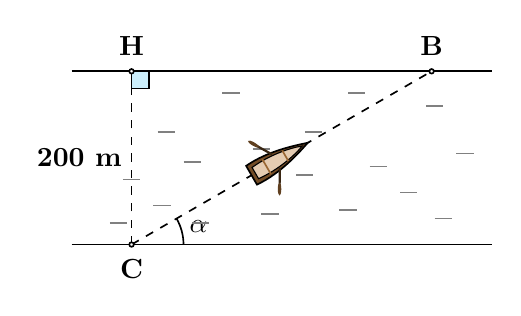
\begin{tikzpicture}[>=stealth, every node/.style={font=\normalsize}, declare function={h=4; goc=30; a=h*sqrt(3);}, scale=0.55]
	% Định nghĩa các điểm
	\path
	(0,0) coordinate (C)
	(0,h) coordinate (H)
	(a,h) coordinate (B)
	(-0.2*a,0) coordinate (B1)
	(1.2*a,0) coordinate (B2)
	(-0.2*a,h) coordinate (H1)
	(1.2*a,h) coordinate (H2)
	;
	% Ký hiệu góc vuông tại H
	\draw[fill=cyan!20, line width=0.6pt] (H) -- ++(0,-0.4) -- ++(0.4,0) -- ++(0,0.4) -- cycle;
	% Vẽ hai bờ sông
	\draw[line width=0.6pt] (B1) -- (B2);
	\draw[line width=0.6pt] (H1) -- (H2);
	% Vẽ các đường đứt nét
	\draw[dashed, line width=0.6pt] (C) -- (H); % Chiều rộng sông
	\draw[dashed, line width=0.6pt] (C) -- (B); % Quãng đường di chuyển
	\draw[dashed, line width=0.6pt] (H) -- (B); % Hình chiếu trên bờ kia
	% Vẽ và ký hiệu góc alpha (với bờ sông)
	\draw[line width=0.6pt] (1.2, 0) arc (0:goc:1.2);
	\node at ({goc/2}:1.6) {$\alpha$};
	% Ghi chú độ dài
	\node[left] at (0, h/2) {\textbf{200 m}};
	% Các đường gợn sóng nước
	\foreach \x/\y in {-0.5/0.5, 0.5/0.9, -0.2/1.5, 1.2/1.9, 0.6/2.6, 2.1/3.5, 1.4/0.5, 3.8/1.6, 2.8/2.2, 4.0/2.6, 5.0/3.5, 4.8/0.8, 6.2/1.2, 7.5/2.1, 6.8/3.2, 5.5/1.8, 3.0/0.7, 7.0/0.6} {
	\draw[gray, line width=0.6pt] (\x,\y) -- ++(0.4,0);
	}
	% Vẽ chiếc thuyền
	\begin{scope}[shift={(a/2, h/2)}, rotate=goc]
	\draw[fill=brown!60!black, line width=0.6pt] (-0.8, 0.25) .. controls (-0.2, 0.3) and (0.4, 0.1) .. (0.7, 0) .. controls (0.4, -0.1) and (-0.2, -0.3) .. (-0.8, -0.25) -- cycle;
	\draw[fill=brown!40, line width=0.4pt] (-0.7, 0.15) .. controls (-0.2, 0.2) and (0.3, 0.1) .. (0.55, 0) .. controls (0.3, -0.1) and (-0.2, -0.2) .. (-0.7, -0.15) -- cycle;
	\draw[line width=0.6pt, brown!80!black] (-0.4, 0.2) -- (-0.4, -0.2);
	\draw[line width=0.6pt, brown!80!black] (0.1, 0.14) -- (0.1, -0.14);
	\draw[line width=0.8pt, brown!30!black] (-0.15, 0.18) -- (-0.4, 0.6);
	\fill[brown!50!black] (-0.4, 0.6) circle [x radius=0.15, y radius=0.04, rotate=120];
	\draw[line width=0.8pt, brown!30!black] (-0.15, -0.18) -- (-0.4, -0.6);
	\fill[brown!50!black] (-0.4, -0.6) circle [x radius=0.15, y radius=0.04, rotate=60];
	\end{scope}
	% Ký hiệu các điểm
	\foreach \t/\pos/\lab in {C/-90/C, H/90/H, B/90/B} {
	\draw[line width=0.6pt, fill=white] (\t) circle (1.5pt) node[shift={(\pos:9pt)}] {$\mathbf{\lab}$};
	}
	\end{tikzpicture}
	}
	\loigiai{
	Trong đó: $BC$ là quãng đường mà thuyền di chuyển\\
	$AB=200m$ là chiều rộng của sông.\\
	$\widehat{ACB}$ là góc tạo bởi phương chuyển động của thuyền với bờ sông\\
	Ta có $BC=200.2=400m$\\
	Xét $\triangle ABC$ vuông tại $A$ có: $\sin \widehat{C}=\dfrac{AB}{BC}=\dfrac{200}{400}=\dfrac{1}{2}$ suy ra $\widehat{C}=30^\circ$.\\
	Vậy góc tạo bởi phương chuyển động của thuyền với bờ sông là $30^\circ$}
\end{ex}
%%==========Câu 43
\begin{ex}%[9H4H1-5]
	%
	Một ngọn đèn đường cao $8m$ đổ bóng dài $6m$ trên mặt đất. Góc tạo bởi nguồn sáng và mặt đất là
	\choice
	{$37^\circ$}
	{\True $53^\circ$}
	{$49^\circ$}
	{$41^\circ$}
	\loigiai{
	Góc tạo bởi tia sáng của ngọn đèn so với mặt đất là $\widehat{C}$\\
	Xét $\triangle ABC$ vuông tại $A$ nên $\tan C=\dfrac{AB}{AC}=\dfrac{8}{6}=\dfrac{4}{3}$ suy ra $\widehat{C}\approx 53^\circ$.\\
	Vậy góc tạo bởi tia sáng của ngọn đèn so với mặt đất khoảng $53^\circ$}
\end{ex}
%%==========Câu 44
\begin{ex}%[9H4H1-5]
	%
	Một chiếc thuyền dự định đi ngang một khúc sông hết $3$ phút với vận tốc $20$ m/phút. Do nước chảy mạnh nên đã đẩy chiếc thuyền lệch so với đường đi dự định một góc $25^\circ$, đoạn đường mà thuyền đã đi lệch so với điểm dự định đến (làm tròn đến chữ số thập phân thứ nhất) là
	\choice
	{\True $28,0m$}
	{$128,7m$}
	{$25,4m$}
	{$54,4m$}
	\loigiai{
	Khi đó $AB$ là chiều rộng của khúc sông và $AB=3.20=60m$\\
	Khi đó $BC$ là quãng đường thực mà thuyền đã di chuyển và $AC$ là đoạn đường thuyền bị lệch so với dự định.\\
	Xét $\triangle ABC$ vuông tại $A$ nên: $\tan B=\dfrac{AC}{AB}$ suy ra $AC=AB.\tan B=60.\tan 25^\circ \approx 28,0m$\\
	Vậy đoạn đường mà nước đã đẩy thuyền đi lệch là $28m$}
\end{ex}
%%==========Câu 45
\begin{ex}%[9H4H1-5]
	%
	\immini[thm]
	{
	Một cái cây có bóng trên mặt đất dài $4,2m$. Cho biết tia nắng qua ngọn cây nghiêng một góc $38^\circ$ so với mặt đất. Chiều cao của cây (làm tròn đến chữ số thập phân thứ 2) là
	\choice
	{$5,37m$}
	{\True $3,28m$}
	{$5,38m$}
	{$3,31m$}
	}
	{
	\begin{tikzpicture}[>=stealth, every node/.style={font=\normalsize}, declare function={a=5; goc=38; b=a*tan(goc); sc=b/5.7;},scale=0.75,transform shape]
	\definecolor{trunkBrown}{HTML}{7B5016}
	\definecolor{leafGreen}{HTML}{76EE2A}
	\definecolor{leafDark}{HTML}{55B11D}
	\definecolor{highlight}{HTML}{A4F66C}
	\path 
	(0,0) coordinate (A)
	(0:a) coordinate (C)
	(90:b) coordinate (B)
	;
	\begin{scope}[shift={(A)}, scale={sc}]
	\begin{scope}[shift={(0, 1.2)}]
	\fill[trunkBrown, draw=black!80!trunkBrown, line width=0.6pt]
	(-0.35,-1.2) .. controls (-0.3,-0.5) and (-0.3,0.5) .. (-0.35,1.2)
	-- (0.35,1.2) .. controls (0.3,0.5) and (0.3,-0.5) .. (0.35,-1.2)
	-- cycle;
	\draw[black!30!trunkBrown, thin] (-0.1, -0.8) -- (-0.1, 0.4);
	\draw[black!30!trunkBrown, thin] (0.1, -0.5) -- (0.1, 0.8);
	\begin{scope}[shift={(0,2.5)}]
	\fill[leafGreen, draw=leafDark!80!black, line width=1pt]
	(0,2) .. controls (0.6,1.8) and (0.8,1.5) .. (1,1.2)
	.. controls (1.5,1.2) and (1.8,0.5) .. (1.8,0)
	.. controls (1.8,-0.8) and (1.2,-1.5) .. (0.5,-1.7)
	.. controls (0.2,-1.8) and (-0.2,-1.8) .. (-0.5,-1.7)
	.. controls (-1.2,-1.5) and (-1.8,-0.8) .. (-1.8,0)
	.. controls (-1.8,0.5) and (-1.5,1.2) .. (-1,1.2)
	.. controls (-0.8,1.5) and (-0.6,1.8) .. (0,2) -- cycle;
	\fill[highlight, opacity=0.6]
	(0.8,1.0) circle (0.4 and 0.25);
	\fill[highlight, opacity=0.4]
	(0,1.2) .. controls (0.3,1.2) and (0.3,1.7) .. (0,1.8)
	.. controls (-0.3,1.7) and (-0.3,1.2) .. (0,1.2);
	\draw[leafDark, opacity=0.4, line width=0.8pt]
	(-0.4, 0.3) .. controls (-0.2, 0.5) and (0.2, 0.5) .. (0.4, 0.3);
	\draw[leafDark, opacity=0.4, line width=0.8pt]
	(-0.8, -0.4) .. controls (-0.5, -0.1) and (0.5, -0.1) .. (0.8, -0.4);
	\draw[leafDark, opacity=0.4, line width=0.8pt]
	(0, -1.0) .. controls (0.2, -0.7) and (0.6, -0.7) .. (0.8, -0.8);
	\end{scope}
	\end{scope}
	\end{scope}
	\draw[line width=1.2pt] (A) -- (B);
	\draw[line width=0.6pt] (B) -- (C) -- (A);
	\path pic[draw, line width=0.6pt, angle radius=7pt]{right angle=B--A--C};
	\path pic[draw, line width=0.6pt, angle radius=16pt]{angle=B--C--A};
	\node[shift={(161:25pt)}] at (C) {$38^\circ$};
	\path (A) -- (C) node[pos=0.5, sloped, above] {$4{,}2\text{ m}$};
	\foreach \t/\pos in {A/225, B/135, C/0}{
	\draw[line width=0.6pt] (\t) circle (0.4pt) node[shift={(\pos:9pt)}] {$\t$};
	}
	\end{tikzpicture}
	}
	\loigiai{
	\immini
	{
	Gọi chiều cao của cái cây là $AB$\\
	Xét $\triangle ABC$ vuông tại $A$ ta có $\tan B=\dfrac{AC}{AB}$\\
	suy ra $AB=BC.\tan B=4,2.\tan 38^\circ \approx 3,28m$\\
	Vậy chiều cao của cái cây là: $3,28m$
	}
	{
%!<\usetikzlibrary{angles,quotes,calc}>
\begin{tikzpicture}[line cap=round, line join=round, >=stealth, font=\footnotesize,scale=0.7]
	% Define coordinates
	\coordinate (A) at (0,0);
	\coordinate (C) at (4.2,0);
	\coordinate (B) at (0,{4.2*tan(38)});
	% Draw the triangle
	\draw (A) -- (B) -- (C) -- cycle;
	% Draw right angle symbol at A
	\draw (0.25,0) -- (0.25,0.25) -- (0,0.25);
	% Draw angle arc and label at C
	\pic[draw, angle radius=7mm, "$38^\circ$", angle eccentricity=1.4] {angle = B--C--A};
	% Label the side AC
	\node[below] at ($(A)!0.5!(C)$) {4,2 m};
	% Draw and label vertices
	\fill (A) circle (1pt) node[below left] {$A$};
	\fill (B) circle (1pt) node[above left] {$B$};
	\fill (C) circle (1pt) node[right] {$C$};
\end{tikzpicture}
	}
	}
\end{ex}
%%==========Câu 46
\begin{ex}%[9H4V1-5]
	%
	\immini[thm]
	{
	Một người đứng cách nơi thả khinh khí cầu $800m$ nhìn thấy nó với góc nghiêng $38^\circ$ so với mặt đất. Biết khoảng cách từ mặt đất đến mắt người đó là $1,5m$, độ cao của khinh khí cầu (làm tròn đến hàng đơn vị) là
	\choice
	{$621m$}
	{$626m$}
	{\True $627m$}
	{$628m$}
	}
	{
\begin{tikzpicture}[>=stealth, every node/.style={font=\normalsize}, declare function={d=5.5; heye=1.5; ang=38; hb=d*tan(ang);},scale=0.5,transform shape]
	\definecolor{byzantium}{rgb}{0.44, 0.16, 0.39}
	\definecolor{brightmaroon}{rgb}{0.76, 0.13, 0.28}
	\definecolor{atomictangerine}{rgb}{1.0, 0.6, 0.4}
	\definecolor{goldenyellow}{rgb}{1.0, 0.87, 0.0}
	\definecolor{arsenic}{rgb}{0.23, 0.27, 0.29}
	\definecolor{antiquebrass}{rgb}{0.8, 0.58, 0.46}
	\definecolor{beaver}{rgb}{0.62, 0.51, 0.44}
	\tikzset{co_vat/.pic={
	\def\T{ 
	(-.7,-2.8)
	..controls +(140:.5) and +(40:.5) ..(1,-2.7)--(.85,-2.8)
	..controls +(-120:1.3) and +(-50:1.3) ..(-.45,-2.9)--cycle
	;
	}
	\fill[arsenic]\T;
	\draw[black]\T;
	\fill[atomictangerine] (-.5,-2.6)
	..controls +(-30:.3) and +(-140:.3) ..(.8,-2.53)
	..controls +(140:.3) and +(60:.3) ..cycle ;
	\draw[beaver] (.65,-2.5)
	..controls +(-90:.2) and +(40:.2) ..(.3,-3.7)
	(.2,-2.5)
	..controls +(-90:.2) and +(40:.2) ..(.05,-3.65)
	(-.7,-2.7)
	..controls +(-70:.4) and +(120:.4) ..(-.15,-3.7)
	;
	\draw (.3,-3.7)--(.05,-3.65)--(-.15,-3.7)--(.05,-3.75)--cycle;
	\draw (.3,-3.7)--(.42,-4.1);
	\draw (.05,-3.65)--(.07,-4);
	\draw (-.15,-3.7)--(-.23,-4.15);
	\draw[fill=antiquebrass] (.42,-4.1)--(.07,-4)--(-.23,-4.15)--(-.24,-4.65)
	--(.1,-4.5)--(.45,-4.55)--cycle;
	\draw[fill=beaver] 
	(-.24,-4.65)--(.1,-4.5)--(.45,-4.55)--(.15,-4.7)--cycle;
	\draw (.1,-4.5)--(.07,-4);
	\def\A{ 
	(-.25,5.5)
	..controls +(-172:4.7) and +(140:6) ..(-.7,-2.8)
	..controls +(140:.5) and +(40:.5) ..(1,-2.7)
	..controls +(45:7) and +(0:3.7) ..cycle
	;
	}
	\draw[black]\A;
	\fill[byzantium] \A;
	\def\Rv{ 
	(-.25,5.5)
	..controls +(0:.4) and +(145:.15) ..(.7,5.3)
	..controls +(170:.2) and +(0:.15) ..(.2,5.35)
	..controls +(-30:.1) and +(110:.05) ..(.42,5.1)
	..controls +(170:.2) and +(20:.2) ..(-.3,5.05)
	--(-.32,4.7)
	..controls +(170:.2) and +(20:.2) ..(-1.23,4.6)
	..controls +(-110:.1) and +(80:.1) ..(-1.32,4.1)
	..controls +(170:.2) and +(20:.2) ..(-2.22,3.95)
	..controls +(-110:.1) and +(90:.15) ..(-2.29,3.38)
	..controls +(170:.2) and +(60:.2) ..(-3.05,3.05)
	..controls +(-92:.1) and +(100:.15) ..(-3.02,2.5)
	..controls +(-170:.1) and +(60:.1) ..(-3.45,2.25)
	..controls +(-85:.1) and +(110:.1) ..(-3.3,1.6)
	..controls +(-170:.1) and +(60:.1) ..(-3.63,1.4)
	..controls +(-80:.1) and +(110:.1) ..(-3.4,.75)
	--(-3.52,.6)
	..controls +(125:.15) and +(-80:.35) ..(-3.9,1.75)
	--(-3.73,1.85)
	..controls +(110:.15) and +(-90:.15) ..(-3.78,2.6)
	..controls +(50:.1) and +(-160:.15) ..(-3.49,2.8)
	..controls +(90:.2) and +(-105:.15) ..(-3.38,3.5)
	..controls +(50:.1) and +(180:.05) ..(-3,3.6)
	..controls +(80:.1) and +(-130:.1) ..(-2.73,4.25)
	..controls +(50:.1) and +(180:.05) ..(-2.08,4.4)
	..controls +(60:.2) and +(-140:.2) ..(-1.7,4.9)
	..controls +(30:.1) and +(180:.1) ..(-1.1,4.95)
	..controls +(60:.2) and +(-140:.2) ..(-.84,5.3)
	..controls +(30:.1) and +(170:.1) ..(-.26,5.3)--cycle
	}
	\draw[black!90,thin]\Rv;
	\fill[brightmaroon] \Rv;
	\def\Or{ 
	(-2.85,-.55)
	--(-2.83,-.3)
	..controls +(120:.1) and +(-70:.1) ..(-3.12,.2)--(-2.85,.45)
	..controls +(120:.1) and +(-70:.1) ..(-3.12,1.05)--(-2.7,1.3)
	..controls +(120:.1) and +(-70:.1) ..(-2.9,1.92)--(-2.15,2.15)
	..controls +(120:.1) and +(-80:.1) ..(-2.27,2.8)
	..controls +(20:.15) and +(-175:.1) ..(-1.31,3)
	..controls +(95:.15) and +(-92:.15) ..(-1.33,3.62)
	..controls +(20:.15) and +(-175:.1) ..(-.33,3.65)--(-.32,4.2)
	..controls +(20:.2) and +(170:.2) ..(.72,4.2)
	..controls +(100:.1) and +(-70:.1) ..(.6,4.7)
	..controls +(20:.2) and +(170:.2) ..(1.4,4.65)
	..controls +(110:.1) and +(-50:.1) ..(1.19,4.95)
	..controls +(20:.15) and +(160:.15) ..(1.9,4.85)
	..controls +(125:.5) and +(0:.6) ..(-.25,5.5)
	..controls +(0:.4) and +(145:.15) ..(.7,5.3)
	..controls +(170:.2) and +(0:.15) ..(.2,5.35)
	..controls +(-30:.1) and +(110:.05) ..(.42,5.1)
	..controls +(170:.2) and +(20:.2) ..(-.3,5.05)
	--(-.32,4.7)
	..controls +(170:.2) and +(20:.2) ..(-1.23,4.6)
	..controls +(-110:.1) and +(80:.1) ..(-1.32,4.1)
	..controls +(170:.2) and +(20:.2) ..(-2.22,3.95)
	..controls +(-110:.1) and +(90:.15) ..(-2.29,3.38)
	..controls +(170:.2) and +(60:.2) ..(-3.05,3.05)
	..controls +(-92:.1) and +(100:.15) ..(-3.02,2.5)
	..controls +(-170:.1) and +(60:.1) ..(-3.45,2.25)
	..controls +(-85:.1) and +(110:.1) ..(-3.3,1.6)
	..controls +(-170:.1) and +(60:.1) ..(-3.63,1.4)
	..controls +(-80:.1) and +(110:.1) ..(-3.4,.75)
	--(-3.52,.6)
	..controls +(-80:.1) and +(125:.35) ..cycle
	}
	\draw[black!90,thin]\Or;
	\fill[atomictangerine] \Or;
	\def\Ye{ 
	(2.8,4.5)--(2.57,4.53)
	..controls +(-50:.1) and +(120:.1) ..(2.82,4.2)
	..controls +(130:.1) and +(0:.1) ..(2.27,4.35)
	..controls +(-50:.1) and +(100:.1) ..(2.45,3.9)
	..controls +(130:.1) and +(0:.1) ..(1.6,4.1)
	..controls +(-60:.1) and +(100:.1) ..(1.7,3.53)
	..controls +(130:.1) and +(0:.1) ..(.78,3.65)
	..controls +(-80:.1) and +(90:.1) ..(.8,3.05)
	..controls +(160:.1) and +(20:.1) ..(-.34,3.05)
	--(-.32,2.45)--(-1.25,2.35)
	..controls +(-80:.1) and +(100:.1) ..(-1.17,1.73)
	..controls +(-150:.15) and +(0:.2) ..(-1.83,.95);
	}
	\draw[black!90,thin]\Ye;
	\fill[goldenyellow] \Ye;
	}}
	\path
	(0,0) coordinate (A)
	(0:d) coordinate (C)
	($(C)+(90:heye)$) coordinate (D)
	(90:heye) coordinate (H)
	($(H)+(90:hb)$) coordinate (B)
	;
	\begin{scope}[shift={(C)}]
	\fill[black!85] (0, heye) circle (0.15);
	\fill[black!85] (-0.05, heye-0.12) -- (0.05, heye-0.12)
	.. controls (0.2, heye-0.2) and (0.2, heye-0.5) .. (0.15, heye-0.8)
	-- (0.08, 0) -- (-0.02, 0) -- (0.02, heye-0.8)
	-- (-0.02, heye-0.8) -- (-0.12, 0) -- (-0.22, 0) -- (-0.15, heye-0.8)
	.. controls (-0.25, heye-0.5) and (-0.25, heye-0.2) .. (-0.05, heye-0.12);
	\fill[black!85, rounded corners=1pt] (-0.15, heye-0.2) -- (-0.25, heye-0.7) -- (-0.15, heye-0.7) -- (-0.05, heye-0.2);
	\fill[black!85, rounded corners=1pt] (0.15, heye-0.2) -- (0.25, heye-0.7) -- (0.15, heye-0.7) -- (0.05, heye-0.2);
	\end{scope}
	\path ($(B)+(0, 0.85)$) pic[scale=0.18] {co_vat};
	\draw[line width=0.6pt] (A) -- (C) -- (D) -- (H) -- cycle;
	\draw[line width=0.6pt] (H) -- (B) -- (D);
	\path pic[draw, line width=0.6pt, angle radius=5pt]{right angle=B--H--D};
	\path pic[draw, line width=1.5pt, color=blue!30!black, angle radius=20pt]{angle=B--D--H};
	\node[shift={(165:30pt)}] at (D) {$38^\circ$};
	\path (C) -- (D) node[midway, right=2pt] {$1,5m$};
	\foreach \t/\pos in {A/225, C/-45, D/0, H/180, B/180}{
	\draw[line width=0.6pt] (\t) circle (0.4pt) node[shift={(\pos:9pt)}] {$\t$};
	}
\end{tikzpicture}
	}
	\loigiai{
	Gọi khoảng cách từ mặt đất đến mắt người đó là $CD=1,5m$\\
	Độ cao của khinh khí cầu là $BA$.\\
	Người đó nhìn khinh khí cầu với góc nghiêng $\widehat{BDH}=38^\circ$.\\
	Khoảng cách từ nơi người đó đứng đến nơi thả khinh khí cầu là $AC=800m$\\
	Và tứ giác $ACDH$ là hình chữ nhật nên $CD=AH=1,5m$\\
	Xét $\triangle BHD$ vuông tại $H$ có: $\tan \widehat{BDH}=\dfrac{BH}{HD}\Rightarrow BH=HD.\tan \widehat{BDH}=800.\tan 38^\circ$\\
	$BA=BH+AH=800.\tan 38^\circ+1,5\approx 627m$\\
	Vậy độ cao của khinh khí cầu là $627m$}
\end{ex}
%%==========Câu 47
\begin{ex}%[9H4V1-5]
	%
	\immini[thm]
	{
	Một người đứng cách tòa nhà cao tầng $62m$, người đó nhìn lên đỉnh tòa nhà với phương nhìn tạo với phương ngang một góc bằng $35^\circ$ và mắt người này cách mặt đất $\text{ 1, }6m$. Chiều cao của tòa nhà (làm tròn đến chữ số thập phân thứ nhất) là
	\choice
	{$\text{ 43,4 }m$}
	{$\text{ 37,2 }m$}
	{$\text{ 52,4 }m$}
	{\True $45,0m$}
	}
	{
%!<\usepackage{amsmath,amssymb}>
%!<\usetikzlibrary{calc,angles,quotes}>

\begin{tikzpicture}[line cap=round, line join=round, >=stealth, thick, scale=0.6, transform shape]
	
	% Các thông số cho toà nhà (dựa trên cấu trúc H1)
	\def\a{1.6}     % Chiều rộng mặt trước
	\def\xd{-0.6}   % Độ lệch x của mặt bên
	\def\dy{0.3}    % Độ lệch y của mặt bên
	\def\h{5.75}    % Chiều cao toà nhà (tính toán theo tỉ lệ: 1.2 + 6.5*tan(35) = 5.75)
	
	% Định nghĩa các điểm hình học
	\coordinate (B) at (0,0);
	\coordinate (C) at (6.5,0);
	\coordinate (D) at (0,1.2);
	\coordinate (M) at (6.5,1.2);
	\coordinate (A) at (0,\h);
	
	% --- VẼ TOÀ NHÀ ---
	
	% Mặt bên (Xanh lơ)
	\fill[cyan!40, draw=black, thick] (-\a,0) -- (-\a+\xd, \dy) -- (-\a+\xd, \h+\dy) -- (-\a, \h) -- cycle;
	% Mặt trước (Trắng)
	\fill[white, draw=black, thick] (-\a,0) rectangle (0,\h);
	% Mặt trên cùng (Đen)
	\fill[black!90, draw=black, thick] (-\a, \h) -- (-\a+\xd, \h+\dy) -- (\xd, \h+\dy) -- (0, \h) -- cycle;
	
	% Dải đen ở mái
	\fill[black!90] (-\a, \h-0.15) rectangle (0, \h);
	\fill[black!90] (-\a, \h-0.15) -- (-\a+\xd, \h-0.15+\dy) -- (-\a+\xd, \h+\dy) -- (-\a, \h) -- cycle;
	
	% Các cửa sổ (Dải ngang màu đen)
	\foreach \y in {0.8, 1.4, 2.0, 2.6, 3.2, 3.8, 4.4, 5.0} {
		% Cửa sổ mặt trước
		\fill[black!90] (-\a, \y) rectangle (0, \y+0.15);
		% Cửa sổ mặt bên
		\fill[black!90] (-\a, \y) -- (-\a+\xd, \y+\dy) -- (-\a+\xd, \y+\dy+0.15) -- (-\a, \y+0.15) -- cycle;
	}
	
	% Cửa chính tầng trệt
	\fill[orange!70!brown, draw=black, thick] (-\a+0.2, 0) rectangle (-0.2, 0.7);
	\fill[black!90] (-\a+0.35, 0) rectangle (-0.85, 0.5);
	\fill[black!90] (-0.75, 0) rectangle (-0.25, 0.5);
	
	% Phần đế móng toà nhà
	\fill[cyan!80!black] (-\a, 0) -- (-\a+\xd, \dy) -- (-\a+\xd, \dy-0.1) -- (-\a, -0.1) -- (0, -0.1) -- (0, 0) -- cycle;
	\draw[black, thick] (-\a, -0.1) -- (0, -0.1) -- (0,0);
	\draw[black, thick] (-\a+\xd, \dy-0.1) -- (-\a, -0.1);
	
	% --- VẼ CÁC ĐƯỜNG NÉT HÌNH HỌC ---
	\draw[thick] (B) -- (C);
	\draw[dashed, thick] (D) -- (M);
	\draw[thick] (A) -- (M);
	
	% --- VẼ NGƯỜI QUAN SÁT ---
	% Vòng tròn màu cam tại mắt M
	\fill[orange!30, opacity=0.8, draw=black, thin] (M) circle (0.28);
	\fill (M) circle (1.5pt);
	
	% Hình dáng người
	\draw[line width=1.5pt] (6.5, 0) -- (6.55, 0.5); % chân trái
	\draw[line width=1.5pt] (6.4, 0) -- (6.5, 0.5); % chân phải
	\draw[line width=3pt, line cap=round] (6.52, 0.5) -- (6.5, 1.0); % thân
	\fill (6.5, 1.1) circle (0.12); % đầu
	\draw[line width=1.2pt] (6.5, 0.95) -- (6.35, 1.05) -- (6.45, 1.2); % tay cầm ống nhòm
	
	% --- NHÃN VÀ GÓC ---
	\node[above] at (A) {\textbf{\textit{A}}};
	\node[below] at (B) {\textbf{\textit{B}}};
	\node[below] at (C) {\textbf{\textit{C}}};
	\node[above right=1pt] at (D) {\textbf{\textit{D}}};
	\node[right=8pt] at (M) {\textbf{\textit{M}}};
	
	\node[above] at ($(B)!0.5!(C)$) {$62 \text{ m}$};
	\node[right] at (6.6, 0.6) {$1,6 \text{ m}$};
	
	% Ký hiệu góc
	\pic [draw, "$35^\circ$", angle radius=1.3cm, angle eccentricity=1.35, font=\small] {angle = A--M--D};
	
\end{tikzpicture}
	}
	\loigiai{
	Gọi $AB$ là chiều cao của tòa nhà, $MC$ là khoảng cách từ mắt của người đứng ngắm đến mặt đất.\\
	Khi đó ta có $MC=DB=1,6m$ và $AB=AD+DB=AD+1,6m$\\
	$\triangle ADM$ vuông tại $D$ nên ta có $\tan M=\dfrac{DM}{AD}$ suy ra $AD=DM.\tan M=62.\tan 35^\circ$\\
	$AB=AD+1,6=62.\tan 35^\circ+1,6\approx 45,0m$\\
	Vậy chiều cao của tòa nhà là $45,0m$}
\end{ex}
%%==========Câu 48
\begin{ex}%[9H4V1-5]
	%
	Chùa Linh Phước thuộc thành phố Đà Lạt là ngôi chùa có kiến trúc độc đáo, các công trình trong khuôn viên chùa được khảm các mảnh sành, sứ, chai bên ngoài nên còn được biết đến với tên gọi khác là chùa Ve Chai. Và đây cũng là ngôi chùa duy nhất ở Việt Nam sở hữu đến 11 kỷ lục, một trong những kỉ lục của chùa đó là \lq\lq ngôi chùa có tháp chuông cao nhất Việt nam\rq\rq được Trung tâm sách kỷ lục Việt Nam ghi nhận vào năm 2008. Một người có tầm mắt cách mặt đất $1,6m$ và đứng cách tháp chuông $50m$ rồi nhìn lên đỉnh tháp với góc nâng khoảng $35^\circ$ thì chiều cao của tháp chuông (làm tròn đến mét) là
	\choice
	{$35m$}
	{$29m$}
	{\True $37m$}
	{$30m$}
	\loigiai{
	Gọi $h$ là chiều cao của tháp chuông, khi đó chiều cao từ tầm mắt người đó đến đỉnh tháp chuông là $h-1,6$.\\
	$CN=50m$ là khoảng cách từ chân tháp đến vị trí người đứng.\\
	$MN$ là khoảng cách từ mặt đất cho đến tầm mắt $MN=1,6m$\\
	Xét $\triangle ABM$ vuông tại $B$ trong đó $\tan \widehat{AMB}=\dfrac{AB}{BM}$ suy ra $\tan 35^\circ=\dfrac{h-1,6}{50}$.\\
	$h-1,6=50.\tan 35^\circ$\\
	$h=50.\tan 35^\circ+1,6\approx 37m$\\
	Vậy, chiều cao của tháp chuông là khoảng $37m$}
\end{ex}
%%==========Câu 49
\begin{ex}%[9H4V1-5]
%
Một người dùng chiếc thang dài $4m$ để trèo lên kiểm tra gác xép của một căn phòng, biết rằng chân thang được đặt hợp với nền phòng một góc $67^\circ$. Chiều cao căn phòng (làm tròn đến chữ số thập phân thứ nhất) là
\choice
{\True $3,7m$}
{$\text{ 4,1 }m$}
{$\text{ 3,6 }m$}
{$\text{ 4,2 }m$}
\loigiai{
Ta có chiều cao của căn phòng là $AB$\\
$\triangle ABC$ vuông tại ta có $\sin C=\dfrac{AB}{BC}$ suy ra $AB=BC.\sin C=4.\sin 67^\circ \approx 3,7m$\\
Vậy chiều cao của căn phòng là $3,7m$}
\end{ex}
%%==========Câu 50
\begin{ex}%[9H4V1-5]
	%
	\immini[thm]
	{
	Trong môn thể thao bóng đá thì \lq\lq khung thành\rq\rq có chiều rộng là $7,32m$ chiều cao là $2,44m$. Vậy khi thực hiện sút quả phạt đền $11m$ thì góc sút sẽ là
	\choice
	{$34^\circ$}
	{$72^\circ$}
	{$18^\circ$}
	{\True $37^\circ$}
	}
	{
	\begin{tikzpicture}[scale=0.35,transform shape, line cap=round, line join=round, >=stealth, font=\footnotesize]
		\coordinate (H) at (0,0);
		\coordinate (N) at (-3.66,0);
		\coordinate (D) at (3.66,0);
		\coordinate (M) at (0,-11);
		\draw (N) -- (D);
		\draw (N) -- (M);
		\draw (D) -- (M);
		\draw (H) -- (M);
		\draw (-0.4,0) -- (-0.4,-0.4) -- (0,-0.4);
		\coordinate (midNH) at (-1.83, 0);
		\coordinate (midHD) at (1.83, 0);
		\draw ($(midNH) + (-0.1,-0.2)$) -- ($(midNH) + (-0.1,0.2)$);
		\draw ($(midNH) + (0.1,-0.2)$) -- ($(midNH) + (0.1,0.2)$);
		\draw ($(midHD) + (-0.1,-0.2)$) -- ($(midHD) + (-0.1,0.2)$);
		\draw ($(midHD) + (0.1,-0.2)$) -- ($(midHD) + (0.1,0.2)$);
		\draw[<->] (-3.66, 1.2) -- (3.66, 1.2) node[midway, above] {$7{,}32\text{ m}$};
		\node[right] at (0, -5.5) {$11\text{ m}$};
		\fill (N) circle (2pt);
		\fill (H) circle (2pt);
		\fill (D) circle (2pt);
		\fill (M) circle (2pt);
		\node[left=2pt] at (N) {$N$};
		\node[above=2pt] at (H) {$H$};
		\node[right=2pt] at (D) {$D$};
		\node[below=2pt] at (M) {$M$};
	\end{tikzpicture}
	}
	\loigiai{
	Ta có $MH=11m$ là khoảng cách từ quả bóng đến khung thành\\
	Suy ra $MH$ là đường trung trực của $ND$ suy ra $NH=DG=\dfrac{7,32}{2}=3,66m$\\
	Khi đó $\triangle NMD$ cân $M$ nên MH là đường phân giác $\widehat{NMD}$, đồng thời $\widehat{NMD}$ chính là góc sút.\\
	Xét $\triangle MNH$ vuông tại $H$ nên $\tan \widehat{NMH}=\dfrac{NH}{MH}=\dfrac{3,66}{11}$ suy ra $\widehat{NMH}\approx 18,4^\circ$ suy ra $\widehat{NMD}\approx 37^\circ$.\\
	Vậy góc sút là $37^\circ$.\\
	}
\end{ex}
\Closesolutionfile{ans}
\indapan{10}{ans/ans-9-B16-TN-D5}
\begin{dang}{Câu thực tế mức độ vận dụng cao}
\end{dang}
\Opensolutionfile{ans}[ans/ans-9-B16-TN-D6]
%%==========Câu 51
\begin{ex}%[9H4C1-5]
	%
	\immini[thm]
	{
	Một chiếc tàu lượn kéo một người chơi dù lượn lên không bằng một sợi dây dài $15m$ và tạo với mặt đất một góc $30^\circ$ (vị trí $C$). Khi tàu lượn tăng tốc độ, độ cao của người này tăng thêm $4m$(vị trí $A$) Khi đó khoảng cách từ người này đến mặt đất (Làm tròn kết quả đến hàng phần mười) là
	\choice
	{$7,5m$}
	{\True $11,5m$}
	{$17,3m$}
	{$13,0m$}
	}
	{\vspace*{-.5cm}
	\begin{tikzpicture}[scale=0.7,transform shape,>=stealth, every node/.style={font=\normalsize}, declare function={
			L = 8;
			gocC = 150;
			yC = L * sin(gocC);
			dy = 4 * (L / 15);
			yA = yC + dy;
			gocA = 180 - asin(yA / L);
		}]
		
		\tikzset{
			dulon/.pic={
				\shade[left color=blue!80, right color=yellow!90, middle color=red!80]
				(-0.6, 0.3) .. controls (-0.6, 0.7) and (0.6, 0.7) .. (0.6, 0.3)
				.. controls (0.4, 0.45) and (-0.4, 0.45) .. cycle;
				\foreach \i in {-0.55, -0.25, 0, 0.25, 0.55} {
					\draw[line width=0.3pt, black!60] (\i, 0.35) -- (0, 0.05);
				}
			}
		}
		
		\path
		(0,0) coordinate (O)
		(gocC:L) coordinate (C)
		(gocA:L) coordinate (A)
		(C |- O) coordinate (D)
		(A |- O) coordinate (B)
		(A |- C) coordinate (H)
		;
		
		\draw[line width=0.6pt] (D) -- (O) (C) -- (D) (A) -- (B) (C) -- (H) (O) -- (C) (O) -- (A);
		
		\path pic[draw, line width=0.6pt, angle radius=5pt]{right angle=O--D--C};
		
		\path pic[draw, line width=0.6pt, angle radius=5pt]{right angle=O--B--A};
		
		\path pic[draw, line width=0.6pt, angle radius=0.8cm]{angle=C--O--D};
		
		\node at (165:1.2) {$30^\circ$};
		
		\foreach \x/\y in {O/C, O/A}{
			\path (\x)--(\y) node[pos=0.5, sloped]{
				\tikz{
					\draw[line width=0.6pt, shift={(-1.5pt,0)}] (-90:2.5pt)--(90:2.5pt);
					\draw[line width=0.6pt, shift={(1.5pt,0)}] (-90:2.5pt)--(90:2.5pt);
				}
			};
		}
		
		\path (C) pic[scale=0.65, rotate=15] {dulon};
		
		\path (A) pic[scale=0.65, rotate=15] {dulon};
		
		\foreach \p/\pos in {O/-45, D/-90, B/-90, C/-135, A/45, H/-45}{
			\draw[line width=0.6pt] (\p) circle (0.4pt) node[shift={(\pos:9pt)}] {$\p$};
		}
		
	\end{tikzpicture}
	}
	\loigiai{
	% TODO: \usepackage{graphicx} required
	\begin{center}
	\begin{tikzpicture}[line cap=round, line join=round, >=stealth, font=\footnotesize, scale=0.45]
		\pgfmathsetmacro{\rad}{15}
		\pgfmathsetmacro{\ang}{30}
		\pgfmathsetmacro{\yc}{\rad*sin(\ang)}
		\pgfmathsetmacro{\xc}{\rad*cos(\ang)}
		\pgfmathsetmacro{\ya}{\yc + 4}
		\pgfmathsetmacro{\xa}{sqrt(\rad*\rad - \ya*\ya)}
		\pgfmathsetmacro{\angOA}{atan(\ya/\xa)}
		\coordinate (O) at (0,0);
		\coordinate (D) at (\xc,0);
		\coordinate (B) at (\xa,0);
		\coordinate (C) at (\xc,\yc);
		\coordinate (H) at (\xa,\yc);
		\coordinate (A) at (\xa,\ya);
		\draw (O) -- (D) -- (C) -- (H);
		\draw (O) -- (A) -- (B);
		\draw (O) -- (C);
		\draw (B) ++(0,0.5) -- ++(0.5,0) -- ++(0,-0.5);
		\draw (D) ++(0,0.5) -- ++(-0.5,0) -- ++(0,-0.5);
		\draw (O) ++(1.5,0) arc (0:\ang:1.5);
		\node at (2.5, 0.6) {$30^\circ$};
		\coordinate (midOA) at ($(O)!0.5!(A)$);
		\draw[shift={(midOA)}, rotate=\angOA] (-0.15,-0.3) -- (-0.15,0.3) (0.15,-0.3) -- (0.15,0.3);
		\node[above left, xshift=-2pt, yshift=2pt] at (midOA) {15 m};
		\coordinate (midOC) at ($(O)!0.5!(C)$);
		\draw[shift={(midOC)}, rotate=\ang] (-0.15,-0.3) -- (-0.15,0.3) (0.15,-0.3) -- (0.15,0.3);
		\node[right, xshift=2pt] at ($(A)!0.5!(H)$) {4 m};
		\fill (O) circle (1.5pt) node[below left] {$O$};
		\fill (A) circle (1.5pt) node[above] {$A$};
		\fill (B) circle (1.5pt) node[below] {$B$};
		\fill (C) circle (1.5pt) node[above right] {$C$};
		\fill (D) circle (1.5pt) node[below] {$D$};
		\fill (H) circle (1.5pt) node[left, xshift=-2pt] {$H$};
		\draw pic[draw,angle radius=2mm] {right angle = B--H--C};
	\end{tikzpicture}
	\end{center}
	Ta có $OA=OC=15m$ là chiều dài dây diều.\\
	$\widehat{AOC}$; $\widehat{COB}$ là góc tạo bởi dây diều với mặt đất, trong đó $\widehat{COB}=30^\circ$\\
	$CD$ là chiều cao ban đầu của diều, $AB$ là chiều cao lúc sau của diều.\\
	Tứ giác $HBDC$ là hình chữ nhật nên $CD=HB$\\
	Xét $\triangle OCD$ vuông tại $D$ nên: $\sin \widehat{COD}=\dfrac{CD}{OC}$ suy ra $CD=OC.\sin \widehat{COD}=15.\sin 30^\circ=7,5m$\\
	Ta có $AB=HB$ $=CD+AH$ $=7,5+4$ $=11,5m$\\
	Vậy Độ cao lúc sau của người đó là: $11,5m$}
\end{ex}
%%==========Câu 52
\begin{ex}%[9H4C1-5]
	%
	Du thuyền AMBASSADOR (sức chứa $500$ khách) là du thuyền $5$ sao lớn nhất trên Vịnh Hạ Long và bắt đầu hoạt động từ năm $2018$. Du thuyền dài $96m$, rộng $14m$ và cao $13m$. Nếu hai người đứng bên bờ biển Hạ Long nhìn ra du thuyền AMBASSADOR, người thứ nhất nhìn ra du thuyền với một góc $30^\circ$ so với bờ biển, người thứ hai nhìn ra du thuyền với một góc $40^\circ$ so với bờ biển, hai người cách nhau $685m$. Khi đó du thuyền đang cách bờ biển là:
	\choice
	{$243,3m$}
	{\True $234,3m$}
	{$324,3m$}
	{$433,2m$}
	\loigiai{
	\begin{center}
	\begin{tikzpicture}[line cap=round, line join=round, >=Stealth, font=\small, scale=1]
		\pgfmathsetmacro{\h}{3.5}
		\pgfmathsetmacro{\bx}{-\h/tan(30)}
		\pgfmathsetmacro{\cx}{\h/tan(40)}
		\coordinate (H) at (0,0);
		\coordinate (A) at (0,\h);
		\coordinate (B) at (\bx,0);
		\coordinate (C) at (\cx,0);
		\draw (A) -- (B) -- (C) -- cycle;
		\draw (A) -- (H);
		\draw (0.25,0) -- (0.25,0.25) -- (0,0.25);
		\draw (B) ++(0.7,0) arc (0:30:0.7);
		\draw (B) ++(0.8,0) arc (0:30:0.8);
		\node at ($(B) + (15:1.35)$) {\textbf{$30^\circ$}};
		\draw (C) ++(-0.8,0) arc (180:140:0.8);
		\node at ($(C) + (160:1.35)$) {\textbf{$40^\circ$}};
		\fill (A) circle (1pt) node[above] {$A$};
		\fill (B) circle (1pt) node[left] {$B$};
		\fill (C) circle (1pt) node[right] {$C$};
		\fill (H) circle (1pt) node[above left] {$H$};
		\draw[<->] ($(B)+(0,-0.6)$) -- ($(C)+(0,-0.6)$) node[midway, below] {\textbf{685 m}};
	\end{tikzpicture}
	\end{center}
	$A$ là vị trí của tàu, $AB$, $AC$ là khoảng cách từ tàu đến hai người.\\
	$AH$ là khoảng cách từ tàu đến bờ biển.\\
	$\triangle ABH$ vuông tại $H$ nên: $BH=AH.\cot B=AH.\cot 30^\circ=AH.\tan60^\circ$ ($\cot 30^\circ=\tan60^\circ$)\\
	$\triangle ACH$ vuông tại $H$ nên: $CH=AH.\cot C=AH.\cot 40^\circ=AH.\tan50^\circ$ ($\cot 40^\circ=\tan50^\circ$)\\
	Ta có $BC=BH+CH=AH.\tan60^\circ+AH.\tan50^\circ=AH.\left(\tan60^\circ+\tan50^\circ\right)$\\
	Suy ra $AH=\dfrac{BC}{\tan60^\circ+\tan50^\circ}=\dfrac{685}{\tan60^\circ+\tan50^\circ}\approx 234,3m$\\
	Vậy du thuyền đang cách bờ biển $234,3m$}
\end{ex}
%%==========Câu 53
\begin{ex}%[9H4C1-5]
	%
	\immini[thm]
	{
	Để xác định được chiều cao của một cây táo, từ hai vị trí cách nhau $\text{ 3,2 }m$ và thẳng hàng với gốc cây, người ta đã dùng dụng cụ để ngắm và xác định được các góc nâng lần lượt là $45^\circ$ và $60^\circ$ (như hình vẽ). Vậy chiều cao của cây táo là
	\choice
	{$4,5m$}
	{\True $7,6m$}
	{$8,2m$}
	{$7,1m$}
	}
	{
\begin{tikzpicture}[
	>=stealth, line join=round,
	every node/.style={font=\normalsize},
	declare function={
		h=5;
		gocA=45;
		gocB=60;
	},scale=0.6,transform shape
	]
	% Định nghĩa các điểm
	\path
	(0, 0) coordinate (C)
	(0, h) coordinate (D)
	({h/tan(gocB)}, 0) coordinate (B)
	({h/tan(gocA)}, 0) coordinate (A);
	
	% VẼ CÂY (Tán lá màu xanh, thân nâu)
	% 1. Thân cây và rễ
	\fill[brown!50!black]
	(-0.4, 0) .. controls (-0.2, 0.5) and (-0.1, 1.5) .. (-0.1, 2.5) --
	(0.1, 2.5) .. controls (0.1, 1.5) and (0.2, 0.5) .. (0.4, 0) -- cycle;
	\fill[brown!50!black]
	(-0.6, 0) .. controls (-0.4, 0.1) .. (-0.3, 0.3) --
	(0.3, 0.3) .. controls (0.4, 0.1) .. (0.6, 0) -- cycle;
	
	% 2. Các cành cây
	\fill[brown!50!black]
	(-0.1, 1.8) .. controls (-0.5, 2.2) .. (-1.2, 2.6) --
	(-1.1, 2.7) .. controls (-0.4, 2.3) .. (0, 2.0) -- cycle;
	\fill[brown!50!black]
	(0.1, 1.5) .. controls (0.6, 1.9) .. (1.3, 2.3) --
	(1.2, 2.4) .. controls (0.5, 2.0) .. (0, 1.7) -- cycle;
	\fill[brown!50!black]
	(-0.05, 2.2) .. controls (-0.2, 2.8) .. (-0.4, 3.5) --
	(-0.25, 3.5) .. controls (-0.1, 2.8) .. (0.05, 2.3) -- cycle;
	\fill[brown!50!black]
	(0.05, 2.0) .. controls (0.3, 2.6) .. (0.6, 3.2) --
	(0.45, 3.3) .. controls (0.2, 2.7) .. (-0.05, 2.1) -- cycle;
	
	% 3. Tán lá cây (Vẽ theo nhiều lớp màu xanh để tạo độ khối)
	% Lớp nền tối
	\fill[green!30!black] (-1.5, 3.0) circle (1.2);
	\fill[green!30!black] (1.5, 2.8) circle (1.3);
	\fill[green!35!black] (0, 3.6) circle (1.4);
	% Lớp giữa
	\fill[green!40!black] (-2.2, 2.6) circle (0.9);
	\fill[green!45!black] (-1.0, 3.8) circle (1.1);
	\fill[green!40!black] (2.0, 2.5) circle (1.0);
	\fill[green!45!black] (1.2, 3.4) circle (1.2);
	\fill[green!50!black] (0, 4.2) circle (0.8);
	% Lớp sáng (điểm nhấn)
	\fill[green!55!black] (-1.8, 2.8) circle (0.7);
	\fill[green!55!black] (1.6, 2.7) circle (0.8);
	\fill[green!60!black] (-0.5, 3.5) circle (1.0);
	\fill[green!60!black] (0.6, 3.3) circle (1.0);
	\fill[green!65!black] (0, 4.4) circle (0.6);
	\fill[green!55!black] (-0.8, 4.2) circle (0.7);
	\fill[green!55!black] (0.8, 4.0) circle (0.7);
	
	% VẼ HÌNH HỌC TÍNH TOÁN
	% Các đoạn thẳng
	\draw[line width=0.6pt] (-0.8, 0) -- (A);
	\draw[line width=0.6pt] (C) -- (D);
	\draw[line width=0.6pt] (D) -- (B);
	\draw[line width=0.6pt] (D) -- (A);
	
	% Ký hiệu góc vuông tại C
	\path pic[draw, line width=0.6pt, angle radius=6pt]{right angle=D--C--A};
	
	% Các đoạn đánh dấu tick trên CD và CB
	\draw[line width=0.6pt] (1.5, -3pt) -- (1.5, 3pt);
	\draw[line width=0.6pt] (-3pt, 2.5) -- (3pt, 2.5);
	
	% Ký hiệu góc và cung tròn
	% Góc 60 độ tại B (1 cung)
	\draw[line width=0.6pt] ($(B)+(-0.5,0)$) arc (180:120:0.5);
	\node at ($(B)+(-0.8, 0.35)$) {$60^\circ$};
	
	% Góc 45 độ tại A (2 cung)
	\draw[line width=0.6pt] ($(A)+(-0.5,0)$) arc (180:135:0.5);
	\draw[line width=0.6pt] ($(A)+(-0.6,0)$) arc (180:135:0.6);
	\node at ($(A)+(-0.95, 0.35)$) {$45^\circ$};
	
	% Nhãn khoảng cách AB
	\path (B) -- (A) node[midway, below] {$3{,}2m$};
	
	% Các điểm và nhãn điểm
	\foreach \p/\pos in {C/-90, B/-90, A/-90, D/90} {
		\draw[line width=0.6pt, fill=black] (\p) circle (0.4pt) node[shift={(\pos:9pt)}] {$\p$};
	}
\end{tikzpicture}
	}
	\loigiai{
	\begin{center}
	\begin{tikzpicture}[
		>=stealth, line join=round,
		every node/.style={font=\normalsize},
		declare function={
			h=5;
			gocA=45;
			gocB=60;
		},scale=0.6,transform shape
		]
		% Định nghĩa các điểm
		\path
		(0, 0) coordinate (C)
		(0, h) coordinate (D)
		({h/tan(gocB)}, 0) coordinate (B)
		({h/tan(gocA)}, 0) coordinate (A);
		
		% VẼ CÂY (Tán lá màu xanh, thân nâu)
		% 1. Thân cây và rễ
		\fill[brown!50!black]
		(-0.4, 0) .. controls (-0.2, 0.5) and (-0.1, 1.5) .. (-0.1, 2.5) --
		(0.1, 2.5) .. controls (0.1, 1.5) and (0.2, 0.5) .. (0.4, 0) -- cycle;
		\fill[brown!50!black]
		(-0.6, 0) .. controls (-0.4, 0.1) .. (-0.3, 0.3) --
		(0.3, 0.3) .. controls (0.4, 0.1) .. (0.6, 0) -- cycle;
		
		% 2. Các cành cây
		\fill[brown!50!black]
		(-0.1, 1.8) .. controls (-0.5, 2.2) .. (-1.2, 2.6) --
		(-1.1, 2.7) .. controls (-0.4, 2.3) .. (0, 2.0) -- cycle;
		\fill[brown!50!black]
		(0.1, 1.5) .. controls (0.6, 1.9) .. (1.3, 2.3) --
		(1.2, 2.4) .. controls (0.5, 2.0) .. (0, 1.7) -- cycle;
		\fill[brown!50!black]
		(-0.05, 2.2) .. controls (-0.2, 2.8) .. (-0.4, 3.5) --
		(-0.25, 3.5) .. controls (-0.1, 2.8) .. (0.05, 2.3) -- cycle;
		\fill[brown!50!black]
		(0.05, 2.0) .. controls (0.3, 2.6) .. (0.6, 3.2) --
		(0.45, 3.3) .. controls (0.2, 2.7) .. (-0.05, 2.1) -- cycle;
		
		% 3. Tán lá cây (Vẽ theo nhiều lớp màu xanh để tạo độ khối)
		% Lớp nền tối
		\fill[green!30!black] (-1.5, 3.0) circle (1.2);
		\fill[green!30!black] (1.5, 2.8) circle (1.3);
		\fill[green!35!black] (0, 3.6) circle (1.4);
		% Lớp giữa
		\fill[green!40!black] (-2.2, 2.6) circle (0.9);
		\fill[green!45!black] (-1.0, 3.8) circle (1.1);
		\fill[green!40!black] (2.0, 2.5) circle (1.0);
		\fill[green!45!black] (1.2, 3.4) circle (1.2);
		\fill[green!50!black] (0, 4.2) circle (0.8);
		% Lớp sáng (điểm nhấn)
		\fill[green!55!black] (-1.8, 2.8) circle (0.7);
		\fill[green!55!black] (1.6, 2.7) circle (0.8);
		\fill[green!60!black] (-0.5, 3.5) circle (1.0);
		\fill[green!60!black] (0.6, 3.3) circle (1.0);
		\fill[green!65!black] (0, 4.4) circle (0.6);
		\fill[green!55!black] (-0.8, 4.2) circle (0.7);
		\fill[green!55!black] (0.8, 4.0) circle (0.7);
		
		% VẼ HÌNH HỌC TÍNH TOÁN
		% Các đoạn thẳng
		\draw[line width=0.6pt] (-0.8, 0) -- (A);
		\draw[line width=0.6pt] (C) -- (D);
		\draw[line width=0.6pt] (D) -- (B);
		\draw[line width=0.6pt] (D) -- (A);
		
		% Ký hiệu góc vuông tại C
		\path pic[draw, line width=0.6pt, angle radius=6pt]{right angle=D--C--A};
		
		% Các đoạn đánh dấu tick trên CD và CB
		\draw[line width=0.6pt] (1.5, -3pt) -- (1.5, 3pt);
		\draw[line width=0.6pt] (-3pt, 2.5) -- (3pt, 2.5);
		
		% Ký hiệu góc và cung tròn
		% Góc 60 độ tại B (1 cung)
		\draw[line width=0.6pt] ($(B)+(-0.5,0)$) arc (180:120:0.5);
		\node at ($(B)+(-0.8, 0.35)$) {$60^\circ$};
		
		% Góc 45 độ tại A (2 cung)
		\draw[line width=0.6pt] ($(A)+(-0.5,0)$) arc (180:135:0.5);
		\draw[line width=0.6pt] ($(A)+(-0.6,0)$) arc (180:135:0.6);
		\node at ($(A)+(-0.95, 0.35)$) {$45^\circ$};
		
		% Nhãn khoảng cách AB
		\path (B) -- (A) node[midway, below] {$3{,}2m$};
		
		% Các điểm và nhãn điểm
		\foreach \p/\pos in {C/-90, B/-90, A/-90, D/90} {
			\draw[line width=0.6pt, fill=black] (\p) circle (0.4pt) node[shift={(\pos:9pt)}] {$\p$};
		}
	\end{tikzpicture}
	\end{center}
	Chiều cao của cái cây là $CD$.\\
	Xét $\triangle ACD$ vuông tại $C$ có $\widehat{CAD}=45^\circ$ nên $\triangle ACD$ vuông cân tại $C$ suy ra $AC=CD$.\\
	$\triangle BCD$ vuông tại $C$ nên: $BC=CD.\cot\widehat{CBD}=CD.\cot60^\circ=CD.\tan 30^\circ$. (Do $\cot60^\circ=\tan 30^\circ$)\\
	Ta có $AC-BC=AB=3,2m$\\
	$CD-CD.\tan 30^\circ=3,2$\\
	$CD.\left(1-\tan 30^\circ\right)=3,2$\\
	$CD=\dfrac{3,2}{1-\tan 30^\circ}\approx 7,6m$\\
	Vậy chiều cao của cây táo là $7,6m$}
\end{ex}
%%==========Câu 54
\begin{ex}%[9H4C1-5]
	%
	Tàu ngầm Kilo Việt Nam cải tiến có khả năng đạt tốc độ $17$ hải lý giờ tương đương $31\text{ km/h }$ khi đi nổi và tối đa $20$ hải lý giờ-tương đương  $37\text{ km/h }~$ khi lặn. Nếu tàu ngầm Kilo đang ở trên mặt biển và lặn xuống rồi di chuyển chéo xuống theo đường thẳng tạo với mặt nước biển một góc $21^\circ$ với tốc độ trung bình của tàu là $9\text{ km/h }$ thì khi ở độ sâu $200m$ tàu đã di chuyển được một khoảng thời gian là (làm tròn kết quả đến giây)
	\choice
	{\True $3$ phút $43$ giây}
	{$3$ phút $16$ giây}
	{$2$ phút $46$ giây}
	{$7$ phút 19 giây}
	\loigiai{
	% TODO: \usepackage{graphicx} required
	\begin{center}
	\begin{tikzpicture}[scale=0.8, line cap=round, line join=round, >=stealth, font=\small]
		\def\AH{8}
		\pgfmathsetmacro{\HB}{\AH * tan(21)}
		\coordinate (A) at (0,0);
		\coordinate (H) at (\AH,0);
		\coordinate (B) at (\AH,-\HB);
		\draw (A) -- (H) -- (B) -- cycle;
		\draw (\AH-0.4, 0) -- (\AH-0.4, -0.4) -- (\AH, -0.4);
		\draw (1.5,0) arc (0:-21:1.5);
		\node at (-10.5:2.1) {$21^\circ$};
		\node[above left] at (A) {${A}$};
		\node[above] at (H) {${H}$};
		\node[below] at (B) {${B}$};
		\node[right] at ($(H)!0.5!(B)$) {$200\text{ m}$};
	\end{tikzpicture}
	\end{center}
	Xét $\triangle AHB$ vuông tại $H$ có.\\
	Quãng đường tàu đi được là: $s=AB=\dfrac{HB}{\sin A}=\dfrac{200}{\sin 21^\circ}m$\\
	Đổi $v=9\text{ km/h }=9000m/\text{ 3600 }s\text{ = }\text{ 2,5m/s }$\\
	Ta có $t=\dfrac{s}{v}=\dfrac{200}{\sin 21^\circ}:2,5\approx 223s$=3 phút 43 giây.\\
	Vậy thời gian tàu lặn xuống độ sâu $200m$ là 3 phút 43 giây}
\end{ex}
%%==========Câu 55
\begin{ex}%[9H4C1-5]
	%
	\immini[thm]
	{
	Hai đài quan sát ở hai vị trí $A$ và $B$ (sát mặt đất) cách nhau $50\mathrm{~km}$ cùng quan sát một chiếc máy bay đang bay trên bầu trời tạo thành các góc $15^\circ$ và $35^\circ$ so với phương ngang (hình vẽ). Khi đó, độ cao của máy bay so với mặt đất là
	\choice
	{$13,84\mathrm{~km}$}
	{$10,70~\mathrm{~km}$}
	{$11,63~\mathrm{~km}$}
	{\True $9,69~\mathrm{~km}$}
	}
	{
	\begin{tikzpicture}[
		>=stealth,
		every node/.style={font=\normalsize},
		declare function={
			c = 10;
			gocA = 15;
			gocB = 35;
		},scale=0.65,transform shape
		]
		\path (0,0) coordinate (A);
		\path (0:c) coordinate (B);
		\path (intersection of A--{$(A)+(gocA:15)$} and B--{$(B)+({180-gocB}:15)$}) coordinate (C);
		\draw[line width=0.6pt] (A) -- (B) -- (C) -- cycle;
		\draw[line width=0.6pt] ($(A)+(0:1.2)$) arc (0:gocA:1.2);
		\draw[line width=0.6pt] ($(A)+(0:1.35)$) arc (0:gocA:1.35);
		\node at ($(A)+({gocA/2}:2)$) {$15^\circ$};
		\draw[line width=0.6pt] ($(B)+(180:1.2)$) arc (180:{180-gocB}:1.2);
		\node at ($(B)+({180-gocB/2}:1.8)$) {$35^\circ$};
		\foreach \p/\pos in {A/225, B/-45}{
			\draw[line width=0.6pt] (\p) circle (0.4pt) node[shift={(\pos:9pt)}] {$\p$};
		}
		\draw[line width=0.6pt] (C) circle (0.4pt);
		\begin{scope}[shift={(C)}, xshift=-25pt, yshift=-5pt, scale=0.1, line join=round, line width=0.6pt]
			\draw[fill=gray!20] (4.83,7.13) .. controls +(0:0) and +(-162:0.3) .. (5.83,7.48 ) .. controls +(24:0.1) and +(170:0.1) .. (6.16,7.5) .. controls +(-10:0.3) and +(169:0.3) .. (7.17,7.31) .. controls +(-10:0.1) and +(36:0.1) .. (7.2,7.17) .. controls +(-144:0.3) and +(0:0) .. (5.97,6.31) (5.01,6.89) .. controls +(0:0) and +(-156:0.2) .. (6.13,7.31) .. controls +(18:0) and +(-18:0) .. (6.12,7.37) .. controls +(171:0.1) and +(0:0) .. (5.72,7.44);
			\draw[fill=gray!15] (10.15,5.45) .. controls +(0:0) and +(-157:0.4) .. (14.3,7.28 ) .. controls +(18:0) and +(-90:0) .. (14.36,7.36) .. controls +(90:0) and +(-95:0.1) .. (14.37,7.76) .. controls +(90:0.1) and +(173:0.1) .. (14.49,7.88 ) .. controls +(-4:0.3) and +(173:0.3) .. (15.61,7.74) .. controls +(-11:0.2) and +(105:0.1) .. (15.83,7.56) .. controls +(-75:0.2) and +(106:0.1) .. (15.97,7.09) .. controls +(-73:0.1) and +(39:0.1) .. (15.89,6.83) .. controls +(-136:0.6) and +(0:0) .. (13.62,4.72) (13.07,4.86) -- (15.79,7.03) -- (15.74,7.11) -- (14.49,7.29) (13.84,7.07) .. controls +(0:0) and +(174:0.2) .. (14.43,7) .. controls +(-7:0.1) and +(27:0.1) .. (14.45,6.9) .. controls +(-156:0.2) and +(23:0.4) .. (13.38,6.42) .. controls +(-158:0.1) and +(-10:0.1) .. (13.22,6.39) .. controls +(170:0.2) and +(0:0) .. (12.57,6.51) (12.07,6.29) .. controls +(0:0) and +(170:0.1) .. (12.63,6.2) .. controls +(-11:0.1) and +(29:0.1) .. (12.63,6.09) .. controls +(-152:0.4) and +(0:0) .. (10.9,5.3);
			\def\than{(6.15,3.69) .. controls +(158:0.7) and +(-41:1) .. (2.33,6.49) .. controls +(140:0.3) and +(-173:0.3) .. (2.43,7) .. controls +(0:0.1) and +(170:0.1) .. (2.8,6.96) .. controls +(-10:2.7) and +(168:3.2) .. (14.21,4.59) .. controls +(-12:1) and +(125:0.9) .. (16.68,3.02) .. controls +(-32:0.4) and +(73:0.3) .. (17.52,1.88 ) .. controls +(-106:0.7) and +(-3:1) .. (14.58,1.13) .. controls +(177:1.9) and +(-22:2.2) .. (6.15,3.69) -- cycle}
			\draw[fill=blue!15] \than;
			\draw[fill=cyan!10] (3.04,6.66) .. controls +(-17:0.1) and +(-97:0.2) .. (5.38,6.29) .. controls +(83:0.2) and +(-54:0.9) .. (3.12,9.47) .. controls +(126:0.1) and +(-6:0.1) .. (2.89,9.62) .. controls +(168:0.2) and +(63:0.1) .. (1.78,9.69) .. controls +(-119:0.1) and +(111:1) .. (2.85,6.84) .. controls +(-67:0.1) and +(162:0.1) .. (3.04,6.66) -- cycle;
			\draw (1.91,9.22) .. controls +(0:0) and +(170:0.1) .. (2.33,9.17) .. controls +(0:0) and +(117:0) .. (2.37,9.13) .. controls +(-66:0.1) and +(111:0.2) .. (3.2,7.01) .. controls +(-63:0) and +(-27:0) .. (3.17,6.97) .. controls +(180:0) and +(-12:0.1) .. (2.79,7.01);
			\draw[fill=cyan!10] (2.81,6.32) .. controls +(-13:0.5) and +(165:0.5) .. (4.52,5.91) .. controls +(-14:0.2) and +(11:0.2) .. (4.58,5.62) .. controls +(-168:0.7) and +(10:0.6) .. (2.13,5.14) .. controls +(-168:0.1) and +(-12:0.1) .. (1.58,5.12) .. controls +(164:0.3) and +(-17:0.3) .. (0.46,5.44) .. controls +(164:0.1) and +(-157:0.1) .. (0.46,5.54) .. controls +(20:0.5) and +(-160:0.6) .. (2.57,6.31) .. controls +(21:0.1) and +(166:0.1) .. (2.81,6.32) -- cycle;
			\draw (2.44,6.26) .. controls +(0:0) and +(165:0.1) .. (2.82,6.16) .. controls +(-11:0.1) and +(14:0) .. (2.83,6.09) .. controls +(-160:0.3) and +(20:0.3) .. (1.29,5.53) .. controls +(-160:0.1) and +(-16:0.1) .. (1.08,5.5) .. controls +(162:0.1) and +(0:0) .. (0.68,5.62);
			\draw[fill=gray!30] (8.89,0.07) .. controls +(174:0.4) and +(-32:0.4) .. (7.25,0.61) .. controls +(148:0.4) and +(-103:0.6) .. (6.8,1.62);
			\draw[fill=gray!30] (9.19,1.54) .. controls +(148:0.4) and +(-21:0.4) .. (8.11,1.98);
			\draw[fill=gray!30] (8.33,0.97) .. controls +(83:0.3) and +(162:0.3) .. (9.19,1.54) .. controls +(-18:0.5) and +(75:0.3) .. (9.6,0.58 ) .. controls +(-105:0.3) and +(-18:0.3) .. (8.85,0.07) .. controls +(162:0.6) and +(-96:0.4) .. (8.33,0.97) -- cycle;
			\draw[fill=gray!40] (8.51,0.92) .. controls +(79:0.3) and +(169:0.3) .. (9.14,1.39) .. controls +(-12:0.4) and +(74:0.4) .. (9.47,0.6) .. controls +(-105:0.2) and +(-4:0.3) .. (8.9,0.2) .. controls +(177:0.3) and +(-100:0.4) .. (8.51,0.92) -- cycle;
			\draw[fill=gray!20] (8.3,2.03) .. controls +(0:0) and +(56:0.1) .. (8.43,1.73) .. controls +(-128:0.2) and +(0:0) .. (7.76,1.88);
			\draw (8.7,1.23) .. controls +(-24:0.2) and +(72:0.2) .. (8.94,0.83) .. controls +(-108:0.2) and +(-13:0.3) .. (8.5,0.64) (8.96,1.38 ) .. controls +(-31:0.2) and +(77:0.2) .. (9.17,0.79) .. controls +(-103:0.3) and +(-4:0.3) .. (8.61,0.36);
			\draw[fill=gray!15] (1.93,0.57) -- (1.49,1.16) -- (1.39,1.25) .. controls +(0:0) and +(-25:0.3) .. (0.17,1.82) .. controls +(157:0.1) and +(97:0.1) .. (0.04,1.71) .. controls +(-79:0.2) and +(114:0.1) .. (0.17,1.27) .. controls +(-68:0.1) and +(150:0.1) .. (0.34,1.09) .. controls +(-27:0.3) and +(161:0.5) .. (1.87,0.42) .. controls +(-16:0.1) and +(-163:0.1) .. (2.25,0.4) .. controls +(14:1.4) and +(-164:1) .. (9.97,2.49) .. controls +(15:0.4) and +(-19:0.4) .. (9.96,2.93) .. controls +(162:0.8 ) and +(-14:0.8 ) .. (6.87,3.79) .. controls +(166:0.2) and +(24:0.2) .. (6.36,3.78 ) .. controls +(-157:1.5) and +(0:0) .. (1.01,1.43);
			\draw (1.89,0.63) -- (9.67,2.99) (1.12,1.48 ) .. controls +(0:0) and +(156:0.1) .. (1.66,1.23) .. controls +(-18:0.1) and +(-162:0.1) .. (1.85,1.23) .. controls +(24:0.2) and +(-155:0.3) .. (3.26,1.85) .. controls +(23:0.1) and +(-27:0.1) .. (3.25,1.97) .. controls +(161:0.2) and +(0:0) .. (2.71,2.18) (3.26,2.42) .. controls +(0:0) and +(162:0.2) .. (3.79,2.21) .. controls +(-18:0.1) and +(-157:0.1) .. (4.01,2.2) .. controls +(23:0.5) and +(-155:0.4) .. (6.51,3.32) .. controls +(23:0.1) and +(-18:0.1) .. (6.52,3.44) .. controls +(163:0.2) and +(0:0) .. (5.97,3.61) (4.7,4.63) -- (13.75,2.22) .. controls +(-11:1.6) and +(-112:0.7) .. (16.9,2.86);
			\draw[fill=blue!30] (13.67,2.81) .. controls +(-102:0.2) and +(100:0.2) .. (13.65,1.84) .. controls +(-82:0.1) and +(-4:0.1) .. (13.53,1.69) -- (12.98,1.82) .. controls +(163:0.1) and +(-84:0.1) .. (12.79,2.02) .. controls +(99:0.3) and +(-111:0.3) .. (12.86,3.04) .. controls +(68:0.1) and +(174:0.1) .. (13.02,3.1) -- (13.56,2.97) .. controls +(-23:0.1) and +(78:0.1) .. (13.67,2.81) -- cycle;
			\draw (17.19,2.58 ) .. controls +(-146:0.4) and +(103:0.6) .. (16.83,1.34) (16.68,3.02) .. controls +(-125:0.7) and +(-2:0.5) .. (15.01,2.41) .. controls +(178:0.5) and +(-174:0.4) .. (14.95,3.01) .. controls +(6:0.5) and +(-133:0.6) .. (16.32,3.45) (15.47,3.06) -- (15.62,2.43) -- (15.63,2.44) (16.1,3.27) -- (16.48,2.79);
			\foreach \x/\y in {7.42/4.28,8.14/4.1,8.83/3.92,9.58/3.73,10.33/3.53,11.93/3.12,11.1/3.33} \draw[fill=white] (\x,\y) ellipse (0.15 and 0.16);
		\end{scope}
	\end{tikzpicture}
	}
	\loigiai{
	\begin{center}
	\begin{tikzpicture}[line cap=round, line join=round, >=stealth, font=\small]
		\coordinate (A) at (0,0);
		\coordinate (B) at (10,0);
		\path[name path=lineA] (A) -- ++(15:12);
		\path[name path=lineB] (B) -- ++(145:8);
		\path[name intersections={of=lineA and lineB, by=C}];
		\coordinate (D) at (C |- A);
		\draw (A) -- (B) -- (C) -- cycle;
		\draw (C) -- (D);
		\draw ($ (D) + (0.3,0) $) -- ($ (D) + (0.3,0.3) $) -- ($ (D) + (0,0.3) $);
		\draw ($(A) + (1.5,0)$) arc (0:15:1.5);
		\node at ($(A) + (2.2,0.3)$) {$15^\circ$};
		\draw ($(B) + (-1.2,0)$) arc (180:145:1.2);
		\node at ($(B) + (-1.8,0.35)$) {$35^\circ$};
		\draw[<->] ($(A) + (0,-0.7)$) -- ($(B) + (0,-0.7)$) node[midway, below] {$50\text{ \text{km}}$};
		\foreach \p in {A,B,C,D} {
			\fill (\p) circle (1.5pt);
		}
		\node[left=3pt] at (A) {$A$};
		\node[right=3pt] at (B) {$B$};
		\node[above=3pt] at (C) {$C$};
		\node[below=3pt] at (D) {$D$};
	\end{tikzpicture}
	\end{center}
	$CD$ là khoảng cách từ máy bay đến mặt đất.\\
	Xét $\triangle ACD$ vuông tại $D$ nên $AD=\dfrac{CD}{\tan 15^\circ}$.\\
	Xét $\triangle BCD$ vuông tại $D$ nên $BD=\dfrac{CD}{\tan 35^\circ}$.\\
	Khi đó $AB=AD+BD=\dfrac{CD}{\tan 15^\circ}+\dfrac{CD}{\tan 35^\circ}=CD\left(\dfrac{1}{\tan 15^\circ}+\dfrac{1}{\tan 35^\circ}\right)$.\\
	$\Rightarrow CD=AB:\left(\dfrac{1}{\tan 15^\circ}+\dfrac{1}{\tan 35^\circ}\right)=50:\left(\dfrac{1}{\tan 15^\circ}+\dfrac{1}{\tan 35^\circ}\right)=9,69~\mathrm{~km}$\\
	Vậy khi đó máy bay đang bay ở độ cao $9,69\mathrm{~km}$}
\end{ex}
%%==========Câu 56
\begin{ex}%[9H4C1-5]
	%
	\immini[thm]
	{
	Một người đang ở trên tầng thượng của một tòa nhà quan sát con đường chạy thẳng đến chân tòa nhà. Anh ta nhìn thấy một người điều khiển ô tô đi về phía tòa nhà với phương nhìn tạo với phương nằm ngang một góc bằng $30^\circ$. Sau $6$ phút, người quan sát vẫn nhìn thấy người điều khiển chiếc ô tô với phương nhìn tạo với phương nằm ngang một góc bằng $60^\circ$. Cho biết vận tốc ô tô không đổi. Thời gian ô tô chạy đến chân tòa nhà là
	\choice
	{$5$ phút}
	{$4,5$ phút}
	{$3,5$ phút}
	{\True $3$ phút}
	}
	{
	\begin{tikzpicture}[line cap=round, line join=round, >=stealth, font=\small,scale=0.5,transform shape]
	\definecolor{carRed}{HTML}{FBC02D}
	\definecolor{carDarkRed}{HTML}{F57F17}
	\definecolor{winBlue}{HTML}{29A0B1}
	\definecolor{lightYel}{HTML}{FFF59D}
	\definecolor{tireGray}{HTML}{4D494D}
	\definecolor{hubGray}{HTML}{7A767A}
	\definecolor{bldgWall}{HTML}{E8755A}
	\definecolor{bldgTrim}{HTML}{7A2A29}
	\definecolor{bldgWin}{HTML}{73D2F3}
	\pgfmathsetmacro{\h}{6}
	\pgfmathsetmacro{\xD}{-\h/tan(60)}
	\pgfmathsetmacro{\xC}{-\h/tan(30)}
	\coordinate (A) at (0,0);
	\coordinate (B) at (0,\h);
	\coordinate (D) at (\xD,0);
	\coordinate (C) at (\xC,0);
	\begin{scope}[shift={(0,0)}]
		\fill[green!70!black] (-1.2, 0) rectangle (1.2, 0.2);
		\fill[bldgWall] (-1.0, 0.2) rectangle (1.0, \h-0.2);
		\fill[gray] (-1.0, 2.5) rectangle (1.0, 2.7);
		\fill[gray] (-1.0, 0.2) rectangle (1.0, 1.2);
		\foreach \x in {-0.7, -0.3, 0.3, 0.7} {
			\foreach \y in {1.5, 2.0, 3.1, 3.7, 4.3, 4.9} {
				\fill[bldgWin] (\x-0.12, \y) rectangle (\x+0.12, \y+0.35);
				\fill[white] (\x-0.12, \y-0.1) rectangle (\x+0.12, \y);
			}
		}
		\fill[brown!60!black] (-0.2, 0.2) rectangle (0.2, 1.2);
		\draw[thick, bldgTrim] (0, 0.2) -- (0, \h);
		\fill[bldgTrim] (-1.1, \h-0.2) rectangle (1.1, \h);
		\fill[bldgTrim] (-1.1, 2.7) rectangle (1.1, 2.9);
		\foreach \x in {-1.1, -0.9, -0.7, -0.5, 0.5, 0.7, 0.9, 1.1} {
			\fill[white] (\x-0.05, 0.2) -- (\x-0.05, 0.6) -- (\x, 0.7) -- (\x+0.05, 0.6) -- (\x+0.05, 0.2) -- cycle;
		}
		\fill[white] (-1.2, 0.35) rectangle (-0.3, 0.45);
		\fill[white] (0.3, 0.35) rectangle (1.2, 0.45);
	\end{scope}
	\draw[thick] (C) -- (A);
	\draw[thick] (C) -- (B);
	\draw[thick] (D) -- (B);
	\newcommand{\drawcar}[1]{
		\begin{scope}[shift={(#1,0)}, scale=0.3]
			\begin{scope}[shift={(-3.4, 0.25)}]
				\fill[carRed, rounded corners=2pt] (-2.4, 0.5) -- (2.4, 0.5) .. controls (3.3, 0.5) and (3.6, 1.0) .. (3.4, 1.6) .. controls (3.2, 2.0) and (2.6, 2.2) .. (2.0, 2.2) -- (1.0, 3.3) -- (-1.9, 3.3) -- (-1.7, 2.8) .. controls (-2.7, 2.5) and (-2.9, 1.0) .. (-2.4, 0.5) -- cycle;
				\fill[winBlue, rounded corners=2pt] (-1.4, 3.1) -- (-0.3, 3.1) -- (0.0, 2.2) -- (-1.5, 2.2) -- cycle;
				\fill[winBlue, rounded corners=2pt] (0.1, 3.1) -- (0.8, 3.1) -- (1.6, 2.2) -- (0.4, 2.2) -- cycle;
				\fill[lightYel] (-2.2, 1.5) .. controls (-2.65, 1.6) and (-2.65, 2.2) .. (-2.2, 2.3) -- cycle;
				\fill[lightYel, rotate around={-35:(3.0, 1.7)}] (3.0, 1.7) ellipse (0.25 and 0.15);
				\fill[carDarkRed, rounded corners=1.5pt] (0.2, 1.5) rectangle (0.8, 1.65);
				\fill[carDarkRed, rounded corners=1.5pt] (2.6, 1.2) rectangle (2.9, 1.3);
				\fill[carDarkRed, rounded corners=1.5pt] (-2.2, 1.2) rectangle (-1.9, 1.3);
				\fill[carDarkRed, rounded corners=2pt] (-1.2, 0.7) rectangle (2.1, 0.85);
				\fill[tireGray] (-1.4, 0.4) circle (0.65);
				\fill[hubGray] (-1.4, 0.4) circle (0.3);
				\fill[tireGray] (1.7, 0.4) circle (0.65);
				\fill[hubGray] (1.7, 0.4) circle (0.3);
			\end{scope}
		\end{scope}
	}
	\drawcar{\xC}
	\drawcar{\xD}
	\draw[thick] (-0.3,0) -- (-0.3,0.3) -- (0,0.3);
	\draw[thick] (C) ++(1.4,0) arc (0:30:1.4);
	\node at ($(C) + (15:2.0)$) {$30^\circ$};
	\draw[thick] (D) ++(0.6,0) arc (0:60:0.6);
	\draw[thick] (D) ++(0.7,0) arc (0:60:0.7);
	\node at ($(D) + (30:1.1)$) {$60^\circ$};
	\fill (A) circle (1.5pt) node[below right] {$A$};
	\fill (B) circle (1.5pt) node[above] {$B$};
	\fill (D) circle (1.5pt) node[below right] {$D$};
	\fill (C) circle (1.5pt);
\end{tikzpicture}
	}
	\loigiai{
	% TODO: \usepackage{graphicx} required
	\begin{center}
	% Giả sử chỉ vẽ khung hình học (điểm, đường thẳng, góc) đại diện cho bài toán thực tế trong hình.
	%!<\usetikzlibrary{calc,angles}>
	
	\begin{tikzpicture}[line cap=round, line join=round, >=stealth, font=\small]
		
		% Define the height of the building (AB)
		\pgfmathsetmacro{\h}{4}
		
		% Define coordinates
		\coordinate (A) at (0,0);
		\coordinate (B) at (0,\h);
		% D is the closer car, angle BDA = 60 degrees
		\coordinate (D) at ({-\h/tan(60)},0);
		% C is the further car, angle BCA = 30 degrees
		\coordinate (C) at ({-\h/tan(30)},0); 
		
		% Draw the main triangle and the line DB
		\draw (C) -- (A) -- (B) -- cycle;
		\draw (D) -- (B);
		
		% Right angle marker at A
		\draw (-0.3,0) -- (-0.3,0.3) -- (0,0.3);
		
		% Angle at the further car (30 degrees, single arc)
		\draw (C) ++(1.2,0) arc (0:30:1.2);
		\node at ($(C) + (15:1.7)$) {$30^\circ$};
		
		% Angle at D (60 degrees, double arc)
		\draw (D) ++(0.5,0) arc (0:60:0.5);
		\draw (D) ++(0.6,0) arc (0:60:0.6);
		\node at ($(D) + (30:1.0)$) {$60^\circ$};
		
		% Draw points and add labels
		\fill (A) circle (1.5pt) node[below right] {$A$};
		\fill (B) circle (1.5pt) node[above] {$B$};
		\fill (D) circle (1.5pt) node[below right] {$D$};
		\fill (C) circle (1.5pt); % Far left point is unlabeled in the image
		
	\end{tikzpicture}
	\end{center}
	Do mặt đất là phương ngang nên $\widehat{BCA}=30^\circ$ và $\widehat{BDA}=60^\circ$.\\
	$AB$ là chiều cao của tòa nhà.\\
	Gọi $x$ (m/phút) là vận tốc ô tô, điều kiện $x > 0$.\\
	Vì ô tô đi từ $C$ đến $D$ trong $6$ phút nên $CD=6x$\\
	Xét $\triangle ABC$ vuông tại $A$, ta có: $\tan \widehat{BCA}=\dfrac{AB}{AC}$ suy ra $AC=\dfrac{AB}{\tan \widehat{BCA}}=\dfrac{AB}{\tan{30^\circ}}=AB\sqrt{3}$. $(1)$\\
	Xét $\triangle ABD$ vuông tại $A$, ta có: $\tan \widehat{BDA}=\dfrac{AB}{AD}$ suy ra $AD=\dfrac{AB}{\tan{60^\circ}}=\dfrac{\sqrt{3}AB}{3}.(2)$\\
	Từ $(1)$ và $(2)$ suy ra $CD=AC-AD=AB\left(\sqrt{3}-\dfrac{\sqrt{3}}{3}\right)=\dfrac{2\sqrt{3}}{3}AB$.\\
	Xét tỉ số $\dfrac{AD}{CD}=\dfrac{\sqrt{3}AB}{3}:\dfrac{2\sqrt{3}}{3}AB=\dfrac{1}{2}$ suy ra $AD=\dfrac{1}{2}CD=\dfrac{1}{2}.6x=3x$\\
	Vậy thời gian để ô tô chạy từ $D$ đến tòa nhà là $\dfrac{3x}{x}=3$ (phút)}
\end{ex}
%%==========Câu 57
\begin{ex}%[9H4C1-5]
	%
	\immini[thm]
	{
	Hai bạn học sinh An và Mai đang đứng ở trên bãi cỏ bằng phẳng, cách nhau $100~m$ thì nhìn thấy một chiếc khinh khí cầu ở vị trí giữa hai bạn(hình minh họa). Biết góc nhìn để nhìn thấy khinh khí cầu (so với phương thẳng đứng) ở vị trí của An là $50^\circ$ và ở vị trí của Mai là $40^\circ$. Khoảng cách của khinh khí cầu so với vị trí An là:
	\choice
	{$64m$}
	{$49m$}
	{\True $77m$}
	{$76m$}
	}
	{
	\begin{tikzpicture}[line cap=round, line join=round, >=stealth, font=\small, scale=0.55]
		\coordinate (A) at (0,0);
		\coordinate (B) at (10,0);
		\path[name path=lineAC] (A) -- ++(40:10);
		\path[name path=lineBC] (B) -- ++(130:10);
		\path[name intersections={of=lineAC and lineBC, by=C}];
		\coordinate (D) at (C |- A);
		\draw (A) -- (B) -- (C) -- cycle;
		\draw (C) -- (D);
		\draw (A) -- ++(0,5.5) node[right, pos=0.9] {x};
		\draw (B) -- ++(0,5.5) node[left, pos=0.9] {y};
		\draw ($(D) + (0.3,0)$) -- ($(D) + (0.3,0.3)$) -- ($(D) + (0,0.3)$);
		\draw (A) ++(90:1) arc (90:40:1);
		\node at ($(A) + (65:1.4)$) {$50^\circ$};
		\draw (B) ++(90:0.9) arc (90:130:0.9);
		\draw (B) ++(90:1.0) arc (90:130:1.0);
		\node at ($(B) + (110:1.4)$) {$40^\circ$};
		\node[below left] at (A) {$A$};
		\node[below right] at (B) {$B$};
		\node[above] at (C) {$C$};
		\node[above left] at (D) {$D$};
		\draw[<->] ($(A) + (0,-0.8)$) -- ($(B) + (0,-0.8)$) node[midway, below] {$100\text{ m}$};
	\end{tikzpicture}
	}
	\loigiai{
	\begin{center}
	\begin{tikzpicture}[line cap=round, line join=round, >=stealth, font=\small, scale=0.55]
		\coordinate (A) at (0,0);
		\coordinate (B) at (10,0);
		\path[name path=lineAC] (A) -- ++(40:10);
		\path[name path=lineBC] (B) -- ++(130:10);
		\path[name intersections={of=lineAC and lineBC, by=C}];
		\coordinate (D) at (C |- A);
		\draw (A) -- (B) -- (C) -- cycle;
		\draw (C) -- (D);
		\draw (A) -- ++(0,5.5) node[right, pos=0.9] {x};
		\draw (B) -- ++(0,5.5) node[left, pos=0.9] {y};
		\draw ($(D) + (0.3,0)$) -- ($(D) + (0.3,0.3)$) -- ($(D) + (0,0.3)$);
		\draw (A) ++(90:1) arc (90:40:1);
		\node at ($(A) + (65:1.4)$) {$50^\circ$};
		\draw (B) ++(90:0.9) arc (90:130:0.9);
		\draw (B) ++(90:1.0) arc (90:130:1.0);
		\node at ($(B) + (110:1.4)$) {$40^\circ$};
		\node[below left] at (A) {$A$};
		\node[below right] at (B) {$B$};
		\node[above] at (C) {$C$};
		\node[above left] at (D) {$D$};
		\draw[<->] ($(A) + (0,-0.8)$) -- ($(B) + (0,-0.8)$) node[midway, below] {$100\text{ m}$};
	\end{tikzpicture}
	\end{center}
	$C$ là vị trí của khinh khí cầu, An ở vị trí $A$, Mai ở vị trí $B$.\\
	$AB=100m$ là khoảng cách giữa An và Mai.\\
	$CD$ khoảng cách từ $AB$ đến khinh khí cầu.\\
	$\widehat{CAx}=50^\circ;\widehat{CBy}=40^\circ$ lần lượt là góc nhìn của An và Mai đến khinh khí cầu so với phương thẳng đứng, suy ra $\widehat{CAB}=40^\circ$; $\widehat{CBA}=50^\circ$.\\
	+Xét $\triangle ACD$ vuông tại $D$ ta có $\tan \widehat{CAD}=\dfrac{CD}{AD}\Rightarrow AD=\dfrac{CD}{\tan \widehat{CAD}}=\dfrac{CD}{\tan 40^\circ}$.\\
	Và $\sin \widehat{CAD}=\dfrac{CD}{AC}\Rightarrow AC=\dfrac{CD}{\sin \widehat{CAD}}=\dfrac{CD}{\sin 40^\circ}$.\\
	+Xét $\triangle CBD$ vuông tại $D$ có $\tan \widehat{CBD}=\dfrac{CD}{BD}\Rightarrow BD=\dfrac{CD}{\tan \widehat{CBD}}=\dfrac{CD}{\tan 50^\circ}$.\\
	Nên $AB=AD+DB=\dfrac{CD}{\tan 40^\circ}+\dfrac{CD}{\tan 50^\circ}=CD\left(\dfrac{1}{\tan 40^\circ}+\dfrac{1}{\tan 50^\circ}\right)$.\\
	$CD=AB:\left(\dfrac{1}{\tan 40^\circ}+\dfrac{1}{\tan 50^\circ}\right)=100:\left(\dfrac{1}{\tan 40^\circ}+\dfrac{1}{\tan 50^\circ}\right)\approx 49,24m$\\
	Suy ra $AC\approx \dfrac{49,24}{\sin 40^\circ}\approx 77m$\\
	Vậy khoảng cách từ An đến khinh khí cầu là $77m$}
\end{ex}
%%==========Câu 58
\begin{ex}%[9H4C1-5]
	%
	\immini[thm]
	{
	Để xác định chiều cao $AH$ của một ngọn núi, người quan sát đứng từ hai vị trí $B$ và $C$ cách nhau $475m$ trên Mặt đất. Tại vị trí $B$, người đó quan sát đỉnh núi với phương nhìn tạo với phương nằm ngang một góc bằng $34^\circ$; tại vị trí $C$, người đó quan sát đỉnh núi với phương nhìn tạo với phương nằm ngang một góc bằng $30^\circ$ (hình vẽ). Biết rằng tầm mắt của người quan sát là $\text{ 1,6 }m$ và giả thiết ba điểm $H$, $B$, $C$ thẳng hàng. Chiều cao của ngọn núi (làm tròn đến đơn vị mét) là
	\choice
	{$1846m$}
	{$2154m$}
	{\True $1906m$}
	{$220m$}
	}
	{
	\begin{tikzpicture}[>=stealth, every node/.style={font=\normalsize}, declare function={h=3.5; he=0.5; angB=34; angC=30; xB=h/tan(angB); xC=h/tan(angC);},scale=0.7,transform shape]
		\definecolor{mygreen}{RGB}{43,106,64}
		\begin{scope}[line join=round]
			\fill[mygreen]
			(-2.5, 0)
			-- (-2.5, 0.8) -- (-2.4, 0.7) -- (-2.4, 1.2) -- (-2.2, 1.0) -- (-2.2, 1.8) -- (-2.1, 1.5)
			-- (-1.6, 2.2) -- (-1.4, 1.8) -- (-1.1, 2.6) -- (-0.8, 2.2)
			-- (-0.4, 3.2) -- (-0.2, 2.8)
			-- (0, h+he)
			-- (0.4, 2.2) -- (0.6, 2.5)
			-- (1.0, 1.4) -- (1.2, 1.8)
			-- (1.8, 0.8) -- (2.0, 1.0)
			-- (3.0, 0)
			-- cycle;
			\fill[white] (-1.5, 0) .. controls (-1.2, 0.8) .. (-0.6, 2.0) .. controls (-0.8, 1.0) and (-1.2, 0.5) .. (-1.1, 0) -- cycle;
			\fill[white] (-0.6, 0) .. controls (-0.4, 1.0) .. (0.2, 2.2) .. controls (0.0, 1.2) and (-0.4, 0.5) .. (-0.2, 0) -- cycle;
			\fill[white] (0.3, 0) .. controls (0.5, 0.7) .. (0.8, 1.4) .. controls (0.6, 0.8) and (0.4, 0.3) .. (0.6, 0) -- cycle;
		\end{scope}
		\path
		(0,0) coordinate (H)
		(0,h+he) coordinate (A)
		(0,he) coordinate (Hp)
		(xB,0) coordinate (B)
		(xC,0) coordinate (C)
		(xB,he) coordinate (Bp)
		(xC,he) coordinate (Cp)
		;
		\draw[line width=0.7pt, mygreen] (-3,0) -- (xC+1,0);
		\draw[line width=0.6pt] (H) -- (A);
		\draw[line width=0.6pt] (B) -- (Bp) -- (A);
		\draw[line width=0.6pt] (C) -- (Cp) -- (A);
		\draw[line width=0.4pt, densely dotted] (-0.2,he) -- (xC+0.5,he);
		\path pic[draw, line width=0.6pt, angle radius=5pt]{right angle=A--H--B};
		\path pic[draw, line width=0.6pt, angle radius=12pt]{angle=A--Bp--Hp};
		\node[shift={(180-angB/2:18pt)}] at (Bp) {$34^\circ$};
		\path pic[draw, line width=0.6pt, angle radius=14pt]{angle=A--Cp--Hp};
		\node[shift={(180-angC/2:20pt)}] at (Cp) {$30^\circ$};
		\foreach \p/\pos in {A/90, H/-90, B/-90, C/-90}{
			\draw[line width=0.6pt] (\p) circle (0.4pt) node[shift={(\pos:9pt)}] {$\p$};
		}
	\end{tikzpicture}
	}
	\loigiai{
	\begin{center}
		\begin{tikzpicture}[line cap=round, line join=round, >=stealth, font=\small,scale=0.7]
			\def\h{6}
			\def\yI{1.2}
			\pgfmathsetmacro{\xD}{\h/tan(34)}
			\pgfmathsetmacro{\xE}{\h/tan(30)}
			\coordinate (H) at (0,0);
			\coordinate (I) at (0,\yI);
			\coordinate (A) at (0,\yI+\h);
			\coordinate (B) at (\xD,0);
			\coordinate (C) at (\xE,0);
			\coordinate (D) at (\xD,\yI);
			\coordinate (E) at (\xE,\yI);
			\draw (A) -- (H) -- (C) -- (E) -- cycle;
			\draw (A) -- (D);
			\draw (I) -- (E);
			\draw (D) -- (B);
			\draw (0, \yI+0.3) -- (0.3, \yI+0.3) -- (0.3, \yI);
			\draw (0, 0.3) -- (0.3, 0.3) -- (0.3, 0);
			\draw (D) ++(-0.6,0) arc (180:146:0.6);
			\node at ($(D) + (-1.0, 0.3)$) {$34^\circ$};
			\draw (E) ++(-0.6,0) arc (180:150:0.6);
			\node at ($(E) + (-1.0, 0.3)$) {$30^\circ$};
			\draw[<->] ($(B) + (0,-0.5)$) -- ($(C) + (0,-0.5)$) node[midway, below] {$475\text{ m}$};
			\node[right] at ($(E)!0.5!(C)$) {$1{,}6\text{ m}$};
			\foreach \p in {A,I,H,D,E,B,C} {
				\fill (\p) circle (1.2pt);
			}
			\node[left=2pt] at (A) {$A$};
			\node[left=2pt] at (I) {$I$};
			\node[left=2pt] at (H) {$H$};
			\node[below left=0pt] at (D) {$D$};
			\node[above=2pt] at (E) {$E$};
			\node[below=2pt] at (B) {$B$};
			\node[below=2pt] at (C) {$C$};
		\end{tikzpicture}
	\end{center}
	So với mặt đất thì $BD$ và $CE$ là phương thẳng đứng; $HC$ và $IE$ là phương ngang nên các tứ giác $IHBD$, $IHCE$, $DBCE$ là hình chữ nhật.\\
	Khi đó ta có $EC=DB=IH=1,6m$; $DE=BC=475m$\\
	+$\triangle AID$ vuông tại $I$ nên: $\tan \widehat{ADI}=\dfrac{AI}{ID}$ suy ra $ID=\dfrac{AI}{\tan \widehat{ADI}}=\dfrac{AI}{\tan 34^\circ}(1)$\\
	+$\triangle AIE$ vuông tại $I$ nên: $\tan \widehat{AEI}=\dfrac{AI}{IE}$ suy ra $IE=\dfrac{AI}{\tan \widehat{AEI}}=\dfrac{AI}{\tan 30^\circ}.(2)$\\
	Từ $(1)$ và $(2)$ suy ra $DE=IE-ID=AI.\left(\dfrac{1}{\tan{30^\circ}}-\dfrac{1}{\tan{34^\circ}}\right)$\\
	$475=AI.\left(\dfrac{1}{\tan{30^\circ}}-\dfrac{1}{\tan{34^\circ}}\right)$ suy ra $AI=475:\left(\dfrac{1}{\tan{30^\circ}}-\dfrac{1}{\tan{34^\circ}}\right)\approx 1903,9m$.\\
	Do đó chiều cao $AH$ của ngọn núi là: $AH=AI+IH\approx 1903,9+1,6\approx 1906m$}
\end{ex}
%%==========Câu 59
\begin{ex}%[9H4C1-5]
	%
	\immini[thm]
	{
	Trên nóc của một tòa nhà có một cột ống khói cao $3m$. Một người đứng trên mặt đất dùng giác kế có chiều cao $1,5m$ so với mặt đất, có thể nhìn thấy đỉnh và chân của ống khói dưới góc $50^\circ$ và $40^\circ$ so với phương nằm ngang. Chiều cao của tòa nhà là
	\choice
	{\True $11,1m$}
	{$7,6m$}
	{$9,6m$}
	{$9,1m$}
	}
	{
	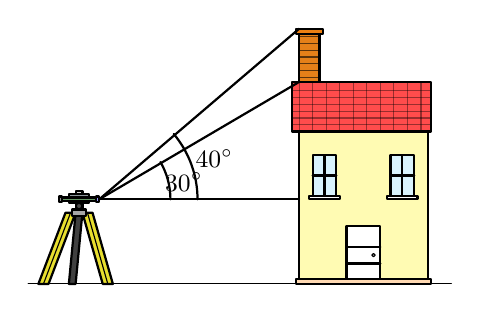
\begin{tikzpicture}[line cap=round, line join=round, >=stealth, font=\small, scale=0.43]
		\pgfmathsetmacro{\dist}{6}
		\pgfmathsetmacro{\yA}{\dist*tan(30)}
		\pgfmathsetmacro{\yB}{\dist*tan(40)}
		\draw[thin, black] (-2, -2.5) -- (10.5, -2.5);
		\begin{scope}
			\fill[yellow!30!white, draw=black, thick] (6.0, -2.5) rectangle (9.8, 2.0);
			\fill[orange!30!white, draw=black, thick] (5.9, -2.5) rectangle (9.9, -2.35);
			\fill[white, draw=black, thick] (7.4, -2.35) rectangle (8.4, -0.8);
			\draw[thick] (7.4, -1.9) -- (8.4, -1.9);
			\draw[thick] (7.4, -1.4) -- (8.4, -1.4);
			\fill[gray!50, draw=black] (8.2, -1.65) circle (0.05);
			\fill[cyan!15!white, draw=black, thick] (6.4, 0.1) rectangle (7.1, 1.3);
			\draw[thick] (6.75, 0.1) -- (6.75, 1.3);
			\draw[thick] (6.4, 0.7) -- (7.1, 0.7);
			\fill[white, draw=black, thick] (6.3, 0.1) rectangle (7.2, 0.0);
			\fill[cyan!15!white, draw=black, thick] (8.7, 0.1) rectangle (9.4, 1.3);
			\draw[thick] (9.05, 0.1) -- (9.05, 1.3);
			\draw[thick] (8.7, 0.7) -- (9.4, 0.7);
			\fill[white, draw=black, thick] (8.6, 0.1) rectangle (9.5, 0.0);
			\fill[orange!60!brown, draw=black, thick] (6.0, \yA) rectangle (6.6, \yB-0.15);
			\foreach \y in {3.6, 3.8, 4.0, 4.2, 4.4, 4.6, 4.8} {
				\draw[black, thin, opacity=0.6] (6.0, \y) -- (6.6, \y);
			}
			\fill[orange!70!brown, draw=black, thick] (5.9, \yB-0.15) rectangle (6.7, \yB);
			\fill[red!70!white, draw=black, thick] (5.8, 2.0) rectangle (9.9, \yA);
			\foreach \y in {2.2, 2.4, 2.6, 2.8, 3.0, 3.2} {
				\draw[black, thin, opacity=0.4] (5.8, \y) -- (9.9, \y);
			}
			\foreach \x in {6.0, 6.4, 6.8, 7.2, 7.6, 8.0, 8.4, 8.8, 9.2, 9.6} {
				\draw[black, thin, opacity=0.4] (\x, 2.0) -- (\x, \yA);
			}
		\end{scope}
		\begin{scope}
			\fill[gray!50!black, draw=black, thick] (-0.6, -0.4) -- (-0.4, -0.4) -- (-0.6, -2.5) -- (-0.8, -2.5) -- cycle;
			\fill[gray!20!yellow, draw=black, thick] (-0.4, -0.4) -- (-0.1, -0.4) -- (0.5, -2.5) -- (0.2, -2.5) -- cycle;
			\draw[black, thin] (-0.25, -0.4) -- (0.35, -2.5);
			\fill[gray!20!yellow, draw=black, thick] (-0.9, -0.4) -- (-0.6, -0.4) -- (-1.4, -2.5) -- (-1.7, -2.5) -- cycle;
			\draw[black, thin] (-0.75, -0.4) -- (-1.55, -2.5);
			\fill[gray!70, draw=black, thick] (-0.7, -0.3) rectangle (-0.3, -0.5);
			\fill[gray!80, draw=black, thick] (-0.6, -0.1) rectangle (-0.4, -0.3);
			\fill[black!70, draw=black] (-0.5, -0.2) circle (0.08);
			\fill[cyan!10!gray, draw=black, thick] (-0.8, -0.1) rectangle (-0.2, 0.15);
			\fill[gray!30, draw=black, thick] (-0.6, 0.15) rectangle (-0.4, 0.25);
			\fill[green!20!gray, draw=black, thick] (-1.0, -0.05) rectangle (0, 0.05);
			\fill[gray!90, draw=black, thick] (-1.1, -0.08) rectangle (-1.0, 0.08);
			\fill[blue!40!white, draw=black, thick] (0, -0.08) rectangle (0.1, 0.08);
		\end{scope}
		\draw[thick, black] (0.1, 0) -- (6.0, 0);
		\draw[thick, black] (0.1, 0) -- (6.0, \yA);
		\draw[thick, black] (0.1, 0) -- (6.0, \yB);
		\draw[thick] (2.2, 0) arc (0:30:2.2);
		\node at (2.6, 0.5) {$30^\circ$};
		\draw[thick] (3.0, 0) arc (0:40:3.0);
		\node at (3.5, 1.2) {$40^\circ$};
		\fill (0,0) circle (0pt) coordinate (O);
		\fill (6.0, 0) circle (0pt) coordinate (H);
		\fill (6.0, \yA) circle (0pt) coordinate (Cbase);
		\fill (6.0, \yB) circle (0pt) coordinate (Ctop);
	\end{tikzpicture}
	}
	\loigiai{
	% TODO: \usepackage{graphicx} required
	\begin{center}
	\begin{tikzpicture}[line cap=round, line join=round, >=stealth, font=\small, scale=0.8]
		\pgfmathsetmacro{\xbase}{2/(tan(40)-tan(30))}
		\pgfmathsetmacro{\h}{1.5}
		\pgfmathsetmacro{\yC}{\h + \xbase*tan(30)}
		\pgfmathsetmacro{\yB}{\h + \xbase*tan(40)}
		\coordinate (D) at (0,0);
		\coordinate (H) at (\xbase,0);
		\coordinate (A) at (0,\h);
		\coordinate (E) at (\xbase,\h);
		\coordinate (C) at (\xbase,\yC);
		\coordinate (B) at (\xbase,\yB);
		\draw (A) -- (D) -- (H) -- (B);
		\draw (A) -- (E);
		\draw (A) -- (C);
		\draw (A) -- (B);
		\draw (0.3,0) -- (0.3,0.3) -- (0,0.3);
		\draw (\xbase-0.3,0) -- (\xbase-0.3,0.3) -- (\xbase,0.3);
		\draw (\xbase-0.3,\h) -- (\xbase-0.3,\h+0.3) -- (\xbase,\h+0.3);
		\draw (A) ++(0:1.3) arc (0:30:1.3);
		\draw (A) ++(0:1.6) arc (0:40:1.6);
		\draw (A) ++(0:1.75) arc (0:40:1.75);
		\node at ($(A) + (15:0.8)$) {$30^\circ$};
		\node at ($(A) + (20:2.3)$) {$40^\circ$};
		\node[left=2pt] at ($(A)!0.5!(D)$) {$1{,}5\text{ m}$};
		\node[right=2pt] at ($(B)!0.5!(C)$) {$2\text{ m}$};
		\foreach \p in {A,B,C,D,E,H} {
			\fill (\p) circle (1.5pt);
		}
		\node[left=2pt] at (A) {$\boldsymbol{A}$};
		\node[below=2pt] at (D) {$\boldsymbol{D}$};
		\node[below=2pt] at (H) {$\boldsymbol{H}$};
		\node[right=2pt] at (E) {$\boldsymbol{E}$};
		\node[right=2pt] at (C) {$\boldsymbol{C}$};
		\node[above=2pt] at (B) {$\boldsymbol{B}$};
	\end{tikzpicture}
	\end{center}
	Gọi $B,C$ là đầu và chân ống khói nên $BC=2m$; $BH$ là chiều cao của tòa nhà.\\
	$AD=1,5m$ là chiều cao của giác kế.\\
	Khi đó tứ giác $ADEH$ là hình chữ nhật nên $EH=AD=1,5m$\\
	$\triangle AEC$ vuông tại $E$, nên: $\tan \widehat{CAE}=\dfrac{CE}{AE}\Rightarrow CE=AE.\tan \widehat{CAE}=AE.\tan 30^\circ$\\
	$\triangle AEB$ vuông tại $E$, nên: $\tan \widehat{BAE}=\dfrac{BE}{AE}$ suy ra $BE=AE.\tan \widehat{BAE}=AE.\tan 40^\circ$.\\
	Nên $BC=BE-CE=AE.\left(\tan 40^\circ-\tan 30^\circ\right)$.\\
	Suy ra $AE=BC:\left(\tan 40^\circ-\tan 30^\circ\right)=2:\left(\tan 40^\circ-\tan 30^\circ\right)=7,6m$\\
	Vậy chiều cao của tòa nhà là: $BH=BC+CE+EH=2+7,6+1,5=11,1m$}
\end{ex}
%%==========Câu 60
\begin{ex}%[9H4C1-5]
	%
	Một chiếc cầu trượt bao gồm phần cầu thang (để bước lên) và phần ống trượt (để trượt xuống) nối liền với nhau. Khi xây dựng, cần thiết kế phần ống trượt nghiêng với mặt đất một góc là $50^\circ$, phần cầu thang cũng đặt nghiêng. Nếu độ dài ống trượt là $3m$, phần cầu thang bước lên có độ dài $2,5m$ thì khoảng cách từ chân cầu thang đến chân ống trượt là (làm tròn kết quả đến hàng phần mười)
	% TODO: \usepackage{graphicx} required
	\begin{center}
	\includegraphics[scale=0.43]{C:/texstudio-man/Anh/{42C895D2-4E84-47B8-B2DE-85E8E33C2854}}
	\end{center}
	\choice
	{$3,2m$}
	{$3,0m$}
	{\True $2,9m$}
	{$2,5m$}
	\loigiai{
	% TODO: \usepackage{graphicx} required
	\begin{center}
	\begin{tikzpicture}[scale=1.5, line cap=round, line join=round, >=stealth, font=\small]
		
		\pgfmathsetmacro{\BC}{3}
		\pgfmathsetmacro{\angC}{50}
		\pgfmathsetmacro{\yB}{\BC * sin(\angC)}
		\pgfmathsetmacro{\xC}{\BC * cos(\angC)}
		\pgfmathsetmacro{\AB}{2.5}
		\pgfmathsetmacro{\xA}{-sqrt(\AB*\AB - \yB*\yB)}
		
		\coordinate (H) at (0,0);
		\coordinate (C) at (\xC,0);
		\coordinate (B) at (0,\yB);
		\coordinate (A) at (\xA,0);
		
		\draw (A) -- (C) -- (B) -- cycle;
		\draw (B) -- (H);
		
		\draw (0.15,0) -- (0.15,0.15) -- (0,0.15);
		
		\draw (C) ++(-0.35,0) arc (180:130:0.35);
		\node at ($(C) + (155:0.6)$) {$50^\circ$};
		
		\node[above left] at ($(A)!0.5!(B)$) {$2{,}5\text{ m}$};
		\node[above right] at ($(B)!0.5!(C)$) {$3\text{ m}$};
		
		\foreach \p in {A, B, C, H} {
			\fill (\p) circle (1pt);
		}
		
		\node[below left] at (A) {$A$};
		\node[above] at (B) {$B$};
		\node[below right] at (C) {$C$};
		\node[below] at (H) {$H$};
		
	\end{tikzpicture}
	\end{center}
	$BC$ là chiều dài cầu trượt; $AC=2,5m$ là chiều dài cầu thang.\\
	$CH$ là khoảng cách từ đỉnh cầu trượt đến mặt sàn.\\
	Xét $\triangle CBH$ vuông tại $H$, ta có:\\
	$\cos \widehat{CBH}=\dfrac{BH}{BC}$ suy ra $BH=BC.\cos \widehat{CBH}=3.\cos{50^\circ}$\\
	$\sin \widehat{CBH}=\dfrac{CH}{BC}$ suy ra $CH=BC.\sin \widehat{CBH}=3.\sin{50^\circ}$\\
	Xét $\triangle CAH$ vuông tại $H$, áp dụng định lý Py-ta-go ta có:\\
	$AH^2=AC^2-CH^2=\left(2,5\right)^2-\left(3.\sin{50^\circ}\right)^2\Rightarrow AH=\sqrt{\left(2,5\right)^2-\left(3.\sin{50^\circ}\right)^2}$\\
	Ta có $AB=AH+BH=\sqrt{\left(2,5\right)^2-\left(3.\sin{50^\circ}\right)^2}+3.\cos{50^\circ}\approx 2,9m$\\
	$\Rightarrow AB=\sqrt{\left(2,5\right)^2-\left(3.\sin{50^\circ}\right)^2}+3.\cos{50^\circ}\approx 2,9m$\\
	Vậy khoảng cách từ chân cầu thang đến chân ống trượt khoảng $2,9m$\\
	}
\end{ex}
\Closesolutionfile{ans}
\indapan{10}{ans/ans-9-B16-TN-D6}
\subsubsection{Bài tập trả lời ngắn}
\begin{dang}{Nhận biết tỉ số lượng giác góc nhọn, tính tỉ số lượng giác của góc nhọn trong tam giác vuông}
\end{dang}
\Opensolutionfile{ans}[ans/ans-9-B16-TLN-D1]
%%==========Câu 61
\begin{ex}%[9H4N1-1]
	%
	Cho $\triangle ABC$ vuông tại $A$, $AB=4\,\text{cm}$, $BC=7\,\text{cm}$. Khi đó $\sin C$ có giá trị là....
	\shortans{$0,57$}
	\loigiai{
	Xét $\triangle ABC$ vuông tại $A$, ta có $\sin C=\dfrac{AB}{BC}=\dfrac{4}{7}$.
	}
\end{ex}
%%==========Câu 62
\begin{ex}%[9H4N1-1]
	%
	Cho $\triangle ABC$ vuông tại $A$, $AB=4\,\text{cm}$, $BC=7\,\text{cm}$. Khi đó $\cos B$ có giá trị là....
	\shortans{$0,57$}
	\loigiai{
	Xét $\triangle ABC$ vuông tại $A$, ta có $\cos B=\dfrac{AB}{BC}=\dfrac{4}{7}$.
	}
\end{ex}
%%==========Câu 63
\begin{ex}%[9H4N1-1]
	%
	Cho $\triangle ABC$ vuông tại $A$, $AB=4\,\text{cm}$, $AC=3\,\text{cm}$. Khi đó $\tan B$ có giá trị là....
	\shortans{$0,75$}
	\loigiai{
	Xét $\triangle ABC$ vuông tại $A$, ta có $\tan B=\dfrac{AC}{AB}=\dfrac{3}{4}$.
	}
\end{ex}
%%==========Câu 64
\begin{ex}%[9H4N1-1]
	%
	Cho $\triangle ABC$ vuông tại $A$, $AB=4\,\text{cm}$, $AC=3\,\text{cm}$. Khi đó $\cot C$ có giá trị là....
	\shortans{$0,75$}
	\loigiai{
	Xét $\triangle ABC$ vuông tại $A$, ta có $\cot C=\dfrac{AC}{AB}=\dfrac{3}{4}$.
	}
\end{ex}
%%==========Câu 65
\begin{ex}%[9H4N1-1]
	%
	Cho $\triangle MNP$ vuông tại $M$, $MN=6\,\text{cm}$, $MP=8\,\text{cm}$. Khi đó $\tan P$ có giá trị là....
	\shortans{$0,75$}
	\loigiai{
	Xét $\triangle MNP$ vuông tại $M$, ta có $\tan P=\dfrac{MN}{MP}=\dfrac{6}{8}=\dfrac{3}{4}$.
	}
\end{ex}
%%==========Câu 66
\begin{ex}%[9H4N1-1]
	%
	Cho $\triangle MNP$ vuông tại $M$, $MN=6\,\text{cm}$, $MP=8\,\text{cm}$. Khi đó $\cot N$ có giá trị là....
	\shortans{$0,75$}
	\loigiai{
	Xét $\triangle MNP$ vuông tại $M$, ta có $\cot N=\dfrac{MN}{MP}=\dfrac{6}{8}=\dfrac{3}{4}$.
	}
\end{ex}
%%==========Câu 67
\begin{ex}%[9H4N1-1]
	%
	Cho $\triangle ABC$ vuông tại $B$, $AB=9\,\text{cm}$, $BC=12\,\text{cm}$. Khi đó $\sin C$ có giá trị là....
	\shortans{$0,6$}
	\loigiai{
	Xét $\triangle ABC$ vuông tại $B$, ta có $AC=\sqrt{9^{2}+12^{2}}=\sqrt{225}=15\,\text{cm}$.\\
	$\sin C=\dfrac{AB}{AC}=\dfrac{9}{15}=\dfrac{3}{5}$.
	}
\end{ex}
%%==========Câu 68
\begin{ex}%[9H4N1-1]
	%
	Cho $\triangle ABC$ vuông tại $B$, $AB=9\,\text{cm}$, $BC=12\,\text{cm}$. Khi đó $\cos B$ có giá trị là....
	\shortans{$0,6$}
	\loigiai{
	Xét $\triangle ABC$ vuông tại $B$, ta có $AC=\sqrt{9^{2}+12^{2}}=\sqrt{225}=15\,\text{cm}$.\\
	$\cos B=\dfrac{AB}{AC}=\dfrac{9}{15}=\dfrac{3}{5}$.
	}
\end{ex}
%%==========Câu 69
\begin{ex}%[9H4N1-1]
	%
	Cho $\triangle OPQ$ vuông ở $P$, đường cao $PH$. Biết $OH=2\,\text{dm}$, $QH=8\,\text{dm}$. Khi đó $\tan O$ có giá trị là....
	\shortans{$2$}
	\loigiai{
	Xét tam giác $OPQ$ vuông tại $P$, đường cao $PH$ ta có: $PH^{2}=OH \cdot QH=2 \cdot 8=16$ suy ra $PH=4\,\text{dm}$.\\
	Xét tam giác $OPH$ vuông tại $H$, ta có $\tan O=\dfrac{PH}{OH}=\dfrac{4}{2}=2$.
	}
\end{ex}
%%==========Câu 70
\begin{ex}%[9H4N1-1]
	%
	Cho $\triangle OPQ$ vuông ở $P$, đường cao $PH$. Biết $OH=2\,\text{dm}$, $QH=8\,\text{dm}$. Khi đó $\cot \widehat{OPH}$ có giá trị là....
	\shortans{$2$}
	\loigiai{
	Xét tam giác $OPQ$ vuông tại $P$, đường cao $PH$ ta có: $PH^{2}=OH \cdot QH=2 \cdot 8=16$ suy ra $PH=4\,\text{dm}$.\\
	Xét tam giác $OPH$ vuông tại $H$, ta có $\cot \widehat{OPH}=\dfrac{PH}{OH}=\dfrac{4}{2}=2$.
	}
\end{ex}
\Closesolutionfile{ans}
\indapan{6}{ans/ans-9-B16-TLN-D1}
\begin{dang}{Nhận biết hai góc phụ nhau. Sử dụng tỉ số lượng giác của hai góc phụ nhau sao sánh, sắp xếp các tỉ số lượng giác}
\end{dang}
\Opensolutionfile{ans}[ans/ans-9-B16-TLN-D2]
%%==========Câu 71
\begin{ex}%[9H4H1-2]
	%
	Giá trị của biểu thức $A=\sin 38^{\circ}-\cos 52^{\circ}$ bằng....
	\shortans{$0$}
	\loigiai{
	Vì $\sin 38^{\circ}=\cos 52^{\circ}$ nên $A=\sin 38^{\circ}-\cos 52^{\circ}=0$.
	}
\end{ex}
%%==========Câu 72
\begin{ex}%[9H4H1-2]
	%
	Giá trị của biểu thức $A=\cot 38^{\circ}-\tan 52^{\circ}$ bằng....
	\shortans{$0$}
	\loigiai{
	Vì $\cot 38^{\circ}=\tan 52^{\circ}$ nên $A=\cot 38^{\circ}-\tan 52^{\circ}=0$.
	}
\end{ex}
%%==========Câu 73
\begin{ex}%[9H4H1-2]
	%
	Giá trị của biểu thức $A=\dfrac{\sin 37^{\circ}+\tan 25^{\circ}}{\cot 65^{\circ}+\cos 53^{\circ}}$ bằng....
	\shortans{$1$}
	\loigiai{
	Vì $\sin 37^{\circ}=\cos 53^{\circ}$; $\cot 65^{\circ}=\tan 25^{\circ}$ nên $A=\dfrac{\sin 37^{\circ}+\tan 25^{\circ}}{\cot 65^{\circ}+\cos 53^{\circ}}=\dfrac{\sin 37^{\circ}+\tan 25^{\circ}}{\tan 25^{\circ}+\sin 37^{\circ}}=1$.
	}
\end{ex}
%%==========Câu 74
\begin{ex}%[9H4H1-2]
	%
	Giá trị của biểu thức $A=\dfrac{\sin 37^{\circ}+\cos 25^{\circ}}{\sin 65^{\circ}+\cos 53^{\circ}}$ bằng....
	\shortans{$1$}
	\loigiai{
	Vì $\sin 37^{\circ}=\cos 53^{\circ}$; $\sin 65^{\circ}=\cos 25^{\circ}$ nên $A=\dfrac{\sin 37^{\circ}+\cos 25^{\circ}}{\sin 65^{\circ}+\cos 53^{\circ}}=\dfrac{\sin 37^{\circ}+\sin 65^{\circ}}{\sin 65^{\circ}+\sin 37^{\circ}}=1$.
	}
\end{ex}
%%==========Câu 75
\begin{ex}%[9H4H1-2]
	%
	Giá trị của biểu thức $A=\tan 27^{\circ}-\cot 63^{\circ}$ bằng....
	\shortans{$0$}
	\loigiai{
	Vì $\tan 27^{\circ}=\cot (90^{\circ}-27^{\circ})=\cot 63^{\circ}$ nên $A=\tan 27^{\circ}-\cot 63^{\circ}=0$.
	}
\end{ex}
%%==========Câu 76
\begin{ex}%[9H4H1-2]
	%
	Giá trị của biểu thức $B=\cos 48^{\circ}-\sin 42^{\circ}$ bằng....
	\shortans{$0$}
	\loigiai{
	Vì $\cos 48^{\circ}=\sin (90^{\circ}-48^{\circ})=\sin 42^{\circ}$ nên $B=\cos 48^{\circ}-\sin 42^{\circ}=0$.
	}
\end{ex}
%%==========Câu 77
\begin{ex}%[9H4H1-2]
	%
	Giá trị của biểu thức $C=\dfrac{\sin 15^{\circ}+\tan 70^{\circ}}{\cos 75^{\circ}+\cot 20^{\circ}}$ bằng....
	\shortans{$1$}
	\loigiai{
	Vì $\sin 15^{\circ}=\cos (90^{\circ}-15^{\circ})=\cos 75^{\circ}$ và $\tan 70^{\circ}=\cot (90^{\circ}-70^{\circ})=\cot 20^{\circ}$.\\
	Nên $C=\dfrac{\sin 15^{\circ}+\tan 70^{\circ}}{\cos 75^{\circ}+\cot 20^{\circ}}=\dfrac{\sin 15^{\circ}+\tan 70^{\circ}}{\sin 15^{\circ}+\tan 70^{\circ}}=1$.
	}
\end{ex}
%%==========Câu 78
\begin{ex}%[9H4H1-2]
	%
	Giá trị của biểu thức $D=\dfrac{\cot 55^{\circ}+\cos 22^{\circ}}{\tan 35^{\circ}+\sin 68^{\circ}}$ bằng....
	\shortans{$1$}
	\loigiai{
	Vì $\cot 55^{\circ}=\tan (90^{\circ}-55^{\circ})=\tan 35^{\circ}$ và $\cos 22^{\circ}=\sin (90^{\circ}-22^{\circ})=\sin 68^{\circ}$.\\
	Nên $D=\dfrac{\cot 55^{\circ}+\cos 22^{\circ}}{\tan 35^{\circ}+\sin 68^{\circ}}=\dfrac{\cot 55^{\circ}+\cos 22^{\circ}}{\cot 55^{\circ}+\cos 22^{\circ}}=1$.
	}
\end{ex}
%%==========Câu 79
\begin{ex}%[9H4H1-2]
	%
	Giá trị của biểu thức $E=\tan 40^{\circ} \cdot \tan 50^{\circ}$ bằng....
	\shortans{$1$}
	\loigiai{
	Vì $\tan 50^{\circ}=\cot (90^{\circ}-50^{\circ})=\cot 40^{\circ}$.\\
	Nên $E=\tan 40^{\circ} \cdot \cot 40^{\circ}=1$.
	}
\end{ex}
\Closesolutionfile{ans}
\indapan{6}{ans/ans-9-B16-TLN-D2}
\begin{dang}{Tính số đo góc, độ dài cạnh trong tam giác vuông}
\end{dang}
\Opensolutionfile{ans}[ans/ans-9-B16-TLN-D3]
%%==========Câu 80
\begin{ex}%[9H4H1-2]
	%
	Cho tam giác $ABC$ vuông tại $A$, biết $AB=12\,\text{cm}$, $BC=15\,\text{cm}$. Số đo góc $B$ (làm tròn đến độ) là....độ
	\shortans{$37$}
	\loigiai{
	Ta có tam giác $ABC$ vuông tại $A$ nên $\cos B=\dfrac{AB}{BC}$ hay $\cos B=\dfrac{12}{15}$.\\
	Vậy $\widehat{B}\approx37^{\circ}$.
	}
\end{ex}
%%==========Câu 81
\begin{ex}%[9H4H1-3]
	%
	Cho tam giác $ABC$ vuông tại $A$, biết $AB=12\,\text{cm}$, $BC=15\,\text{cm}$. Số đo góc $C$ (làm tròn đến độ) là....độ
	\shortans{$53$}
	\loigiai{
	Ta có tam giác $ABC$ vuông tại $A$ nên $\sin C=\dfrac{AB}{BC}$ hay $\sin C=\dfrac{12}{15}$.\\
	Vậy $\widehat{C}\approx53^{\circ}$.
	}
\end{ex}
%%==========Câu 82
\begin{ex}%[9H4H1-3]
	%
	Cho tam giác $ABC$ vuông tại $A$, biết $\widehat{B}=60^{\circ}$, $BC=7\,\text{cm}$. Độ dài cạnh $AC$ là ....
	\shortans{$6,06$}
	\loigiai{
	Xét tam giác $ABC$ vuông tại $A$, ta có: $\sin B=\dfrac{AC}{BC}$.\\
	$AC=BC \cdot \sin B=7 \cdot \sin 60^{\circ}=\dfrac{7\sqrt{3}}{2}\,(\text{cm})$.
	}
\end{ex}
%%==========Câu 83
\begin{ex}%[9H4H1-3]
	%
	Cho tam giác $ABC$ vuông tại $A$, biết $\widehat{B}=60^{\circ}$, $BC=7\,\text{cm}$. Độ dài cạnh $AB$ là ....
	\shortans{$3,5$}
	\loigiai{
	Xét tam giác $ABC$ vuông tại $A$, ta có: $\cos B=\dfrac{AB}{BC}$.\\
	$AB=BC \cdot \cos B=7 \cdot \cos 60^{\circ}=3,5\,(\text{cm})$.
	}
\end{ex}
%%==========Câu 84
\begin{ex}%[9H4H1-3]
	%
	Một cái thang dài $4\,\text{m}$ tựa vào tường làm thành góc $63^{\circ}$ với mặt đất. Khoảng cách từ chân thang đến tường (làm tròn đến $2$ chữ số thập phân) là.....
	\shortans{$1,82$}
	\loigiai{
	Gọi chiếc thang là $BC=4\,\text{m}$, bức tường là $AC$, góc tạo bởi thang và mặt đất là $\widehat{B}=63^{\circ}$.\\
	Ta có tam giác $ABC$ vuông tại $A$ nên $\cos B=\dfrac{AB}{BC}$.\\
	Suy ra $AB=BC \cdot \cos B=4 \cdot \cos 63^{\circ}\approx1,816\,\text{m}$.
	}
\end{ex}
%%==========Câu 85
\begin{ex}%%[9H4H1-5]
	%
	Một cái thang dài $4\,\text{m}$ tựa vào tường làm thành góc $63^{\circ}$ với mặt đất. Vậy chiều cao của bức tường (làm tròn đến $2$ chữ số thập phân) là........
	\shortans{$3,56$}
	\loigiai{
	Gọi chiếc thang là $BC=4\,\text{m}$, chiều cao bức tường là $AC$, góc tạo bởi thang và mặt đất là $\widehat{B}=63^{\circ}$.\\
	Ta có tam giác $ABC$ vuông tại $A$ nên $\sin B=\dfrac{AC}{BC}$.\\
	Suy ra $AC=BC \cdot \sin B=4 \cdot \sin 63^{\circ}\approx3,564\,(\text{m})$.
	}
\end{ex}
%%==========Câu 86
\begin{ex}%%[9H4H1-5]
	%
	\immini[thm]
	{
	Anh Toàn lái xe trên con đường xuống dốc có biển cảnh báo độ dốc $6\%$. Ban đầu anh ở vị trí $A$ cao $35\,\text{m}$ so với mực nước biển. Hỏi sau khi lái xe xuống dốc được quãng đường $300\,\text{m}$ (vị trí $B$) thì vị trí này cao .......... mét so với mực nước biển (làm tròn đến hàng đơn vị).
	}
	{
	\begin{tikzpicture}[line cap=round, line join=round, >=stealth, scale=0.5]
		\definecolor{carMain}{HTML}{FFC000}
		\definecolor{winBlue}{HTML}{29A0B1}
		\definecolor{lightYel}{HTML}{FFFFBB}
		\definecolor{tireGray}{HTML}{4D494D}
		\definecolor{hubGray}{HTML}{7A767A}
		\coordinate (H) at (0,0);
		\coordinate (B) at (10,0);
		\coordinate (A) at (0,3);
		\draw[thick] (H) -- (B) -- (A) -- cycle;
		\pic [draw, thick, green!30!black, "$\alpha$", angle radius=1.2cm, angle eccentricity=1.3] {angle = A--B--H};
		\fill[blue] (H) circle (2pt) node[black, left=2pt] {$H$};
		\fill[blue] (B) circle (2pt) node[black, below right] {$B$};
		\fill[blue] (A) circle (2pt) node[black, left=2pt] {$A$};
		\pgfmathsetmacro{\carangle}{atan2(-3,10)}
		\coordinate (CarPos) at ($(A)!0.2!(B)$);
		\begin{scope}[shift={(CarPos)}, rotate=\carangle]
			\begin{scope}[scale=0.35, shift={(0, 0.25)}]
				\fill[carMain, rounded corners=2pt] (-2.4, 0.5)
				-- (2.4, 0.5)
				.. controls (3.3, 0.5) and (3.6, 1.0) .. (3.4, 1.6)
				.. controls (3.2, 2.0) and (2.6, 2.2) .. (2.0, 2.2)
				-- (1.0, 3.3)
				-- (-1.9, 3.3)
				-- (-1.7, 2.8)
				.. controls (-2.7, 2.5) and (-2.9, 1.0) .. (-2.4, 0.5)
				-- cycle;
				\fill[winBlue, rounded corners=2pt]
				(-1.4, 3.1) -- (-0.3, 3.1) -- (0.0, 2.2) -- (-1.5, 2.2) -- cycle;
				\fill[winBlue, rounded corners=2pt]
				(0.1, 3.1) -- (0.8, 3.1) -- (1.6, 2.2) -- (0.4, 2.2) -- cycle;
				\fill[winBlue] (-2.2, 1.5) .. controls (-2.65, 1.6) and (-2.65, 2.2) .. (-2.2, 2.3) -- cycle;
				\fill[lightYel, rotate around={-35:(3.0, 1.7)}] (3.0, 1.7) ellipse (0.25 and 0.15);
				\fill[black!60, rounded corners=1.5pt] (0.2, 1.5) rectangle (0.8, 1.65);
				\fill[orange, rounded corners=1.5pt] (2.6, 1.2) rectangle (2.9, 1.3);
				\fill[red, rounded corners=1.5pt] (-2.2, 1.2) rectangle (-1.9, 1.3);
				\fill[black!60, rounded corners=2pt] (-1.2, 0.7) rectangle (2.1, 0.85);
				\fill[tireGray] (-1.4, 0.4) circle (0.65);
				\fill[hubGray] (-1.4, 0.4) circle (0.3);
				\fill[tireGray] (1.7, 0.4) circle (0.65);
				\fill[hubGray] (1.7, 0.4) circle (0.3);
			\end{scope}
		\end{scope}
	\end{tikzpicture}
	}
	\shortans{$17$}
	\loigiai{
	Gọi $\alpha$ là góc tạo bởi con dốc và phương nằm ngang.\\
	$6 \%=\dfrac{A H}{B H} \cdot 100 \%$\\
	Thì ta có: $\tan \alpha = 0,06$ suy ra $\alpha\approx3^{\circ}26'$.\\
	Gọi $AH$ là độ cao giảm xuống sau khi đi hết dốc $AB$. Ta có $AH = AB \cdot \sin \alpha \approx 300 \cdot \sin 3^{\circ}26' \approx 18\,\text{m}$.\\
	Do đó, ở vị trí $B$, xe anh Toàn cao khoảng $35-18=17\,\text{m}$ so với mực nước biển.
	}
\end{ex}
%%==========Câu 87
\begin{ex}%[9H4H1-5]
%
Một chiếc thang đơn khi dựa vào tường thì góc $\alpha$ giữa thang và mặt đất được khuyến cáo nằm trong khoảng từ $60^{\circ}$ đến $65^{\circ}$ thì an toàn. Biết chiều dài thang là $6\,\text{m}$. Khoảng cách $x\,(\text{m})$ từ chân thang đến chân tường theo lý thuyết nhỏ nhất là(làm tròn tới hàng phần trăm)
\shortans{$2,54$}
\loigiai{
Gọi chiều dài chiếc thang là $BC=6\,\text{m}$, chiều cao bức tường là $AB$, góc tạo bởi thang và mặt đất là $\widehat{C}=\alpha^{\circ}$.\\
Ta có tam giác $ABC$ vuông tại $A$ nên $\cos C=\dfrac{AC}{BC}$ suy ra $AC=BC \cdot \cos C=6 \cdot \cos \alpha$.\\
Mà $60^{\circ}\le\alpha\le65^{\circ}$ nên $\cos 60^{\circ}\ge \cos \alpha\ge \cos 65^{\circ}$ suy ra $6 \cdot \cos 60^{\circ}\ge6 \cdot \cos \alpha\ge6 \cdot \cos 65^{\circ}$.\\
Suy ra $3\,\text{m}\ge AC\ge2,54\,\text{m}$.\\
Vậy, để đảm bảo an toàn thì nên đặt chân thang cách chân tường khoảng từ $2,54\,\text{m}$ đến $3\,\text{m}$.
}
\end{ex}
\Closesolutionfile{ans}
\indapan{6}{ans/ans-9-B16-TLN-D3}
\begin{dang}{Tính giá trị biểu thức liên quan đến tỉ số lượng giác}
\end{dang}
\Opensolutionfile{ans}[ans/ans-9-B16-TLN-D4]
%%==========Câu 88
\begin{ex}%[9H4N1-4]
%
Cho góc nhọn $\alpha$. Biết $\cot \alpha=2$ khi đó $\tan \alpha$ có giá trị là$\ldots$
\shortans{$0,5$}
\loigiai{
Vì $\tan \alpha \cdot \cot \alpha=1$ nên ta có $\tan \alpha=\dfrac{1}{\cot \alpha}=\dfrac{1}{2}$.
}
\end{ex}
%%==========Câu 89
\begin{ex}%[9H4N1-4]
	%
	Cho góc nhọn $\alpha$. Biết $\tan \alpha=\sqrt{3}$, khi đó $\cot \alpha$ có giá trị là$\ldots$(làm tròn đến số thập phân thứ 2)
	\shortans{$0,58$}
	\loigiai{
	Vì $\tan \alpha \cdot \cot \alpha = 1$ nên ta có $\cot \alpha = \dfrac{1}{\tan \alpha} = \dfrac{1}{\sqrt{3}}$.
	}
\end{ex}
%%==========Câu 90
\begin{ex}%[9H4N1-4]
	%
	Cho góc nhọn $\alpha$. Biết $\cos \alpha = 0{,}6$, khi đó $\sin \alpha$ có giá trị là$\ldots$
	\shortans{$0,8$}
	\loigiai{
	Ta có $\sin^2 \alpha + \cos^2 \alpha = 1$ nên $\sin \alpha = \sqrt{1 - (0{,}6)^2} = \sqrt{0{,}64} = 0{,}8$.
	}
\end{ex}
%%==========Câu 91
\begin{ex}%[9H4N1-4]
	%
	Cho góc nhọn $\alpha$. Biết $\tan \alpha = \sqrt{3}$, khi đó $\cos \alpha$ có giá trị là$\ldots$
	\shortans{$0,5$}
	\loigiai{
	Ta có $1 + \tan^2 \alpha = \dfrac{1}{\cos^2 \alpha}$ \\
	suy ra $\cos^2 \alpha = \dfrac{1}{1 + \tan^2 \alpha} = \dfrac{1}{1 + (\sqrt{3})^2} = \dfrac{1}{4}$ \\
	suy ra $\cos \alpha = \dfrac{1}{2}$.
	}
\end{ex}
%%==========Câu 92
\begin{ex}%[9H4C1-4]
	%
	Cho góc nhọn $\alpha$. Giá trị biểu thức $A = \sin^4 \alpha + \cos^4 \alpha + 2 \sin^2 \alpha \cdot \cos^2 \alpha$ bằng$\ldots$
	\shortans{$1$}
	\loigiai{
	\begin{align*}
	A &= \sin^4 \alpha + \cos^4 \alpha + 2 \sin^2 \alpha \cdot \cos^2 \alpha \\
	A &= \left(\sin^2 \alpha\right)^2 + 2 \sin^2 \alpha \cdot \cos^2 \alpha + \left(\cos^2 \alpha\right)^2 \\
	A &= \left(\sin^2 \alpha + \cos^2 \alpha\right)^2 \\
	A &= 1^2 = 1.
	\end{align*}
	}
\end{ex}
%%==========Câu 93
\begin{ex}%[9H4C1-4]
	%
	Cho góc nhọn $\alpha$. Giá trị biểu thức $B = \sin^6 \alpha + \cos^6 \alpha + 3 \sin^2 \alpha \cdot \cos^2 \alpha$ bằng...
	\shortans{$1$}
	\loigiai{
	\begin{align*}
	B &= \sin^6 \alpha + \cos^6 \alpha + 3 \sin^2 \alpha \cdot \cos^2 \alpha \\
	B &= \left(\sin^2 \alpha\right)^3 + \left(\cos^2 \alpha\right)^3 + 3 \sin^2 \alpha \cdot \cos^2 \alpha \\
	B &= \left(\sin^2 \alpha + \cos^2 \alpha\right)\left(\sin^4 \alpha - \sin^2 \alpha \cdot \cos^2 \alpha + \cos^4 \alpha\right) + 3 \sin^2 \alpha \cdot \cos^2 \alpha \\
	B &= 1 \cdot \left(\sin^4 \alpha - \sin^2 \alpha \cdot \cos^2 \alpha + \cos^4 \alpha\right) + 3 \sin^2 \alpha \cdot \cos^2 \alpha \\
	B &= \sin^4 \alpha + 2 \cdot \sin^2 \alpha \cdot \cos^2 \alpha + \cos^4 \alpha \\
	B &= \left(\sin^2 \alpha + \cos^2 \alpha\right)^2 \\
	B &= 1^2 = 1.
	\end{align*}
	}
\end{ex}
%%==========Câu 94
\begin{ex}%[9H4C1-4]
	%
	Cho góc nhọn $\alpha$ và $\tan \alpha = \dfrac{1}{2}$. Khi đó biểu thức $A = 2 \sin \alpha + \cos \alpha + \sin \alpha \cdot \cos \alpha$ có giá trị là (lấy kết quả đến chữ số thập phân thứ hai)$\ldots$
	\shortans{$2,19$}
	\loigiai{
	Vì $1 + \tan^2 \alpha = \dfrac{1}{\cos^2 \alpha}$ nên khi $\tan \alpha = \dfrac{1}{2}$ thì $1 + \left(\dfrac{1}{2}\right)^2 = \dfrac{5}{4} = \dfrac{1}{\cos^2 \alpha}$. \\
	Suy ra $\cos^2 \alpha = \dfrac{4}{5} \quad\text{suy ra}\quad \cos \alpha = \dfrac{2 \sqrt{5}}{5}$. \\
	Và $\tan \alpha = \dfrac{\sin \alpha}{\cos \alpha} \quad\text{suy ra}\quad \sin \alpha = \tan \alpha \cdot \cos \alpha = \dfrac{1}{2} \cdot \dfrac{2 \sqrt{5}}{5} = \dfrac{\sqrt{5}}{5}$. \\
	Khi đó $A = 2 \cdot \dfrac{\sqrt{5}}{5} + \dfrac{2 \sqrt{5}}{5} + \dfrac{\sqrt{5}}{5} \cdot \dfrac{2 \sqrt{5}}{5} = \dfrac{4 \sqrt{5} + 2}{5} \approx 2{,}19$. \\
	Vậy biểu thức $A \approx 2{,}19$.
	}
\end{ex}
%%==========Câu 95
\begin{ex}%[9H4C1-4]
	%
	Với góc nhọn $\alpha$, khi đó biểu thức $B = 3 \sin^2 \alpha + \dfrac{3}{1 + \tan^2 \alpha} - 2$ có giá trị là$\ldots$
	\shortans{$1$}
	\loigiai{
	\begin{align*}
	B &= 3 \sin^2 \alpha + \dfrac{3}{1 + \tan^2 \alpha} - 2 \\
	&= 3 \sin^2 \alpha + \dfrac{3}{\dfrac{1}{\cos^2 \alpha}} - 2 \\
	&= 3 \sin^2 \alpha + 3 \cos^2 \alpha - 2 \\
	&= 3 \left(\sin^2 \alpha + \cos^2 \alpha\right) - 2 \\
	&= 3 - 2 = 1.
	\end{align*}
	Vậy $B = 3 \sin^2 \alpha + \dfrac{3}{1 + \tan^2 \alpha} - 2$ có giá trị bằng $1$.
	}
\end{ex}
\Closesolutionfile{ans}
\indapan{6}{ans/ans-9-B16-TLN-D4}
\begin{dang}{Bài toán thực tế mức độ vận dụng}\end{dang}
\Opensolutionfile{ans}[ans/ans-9-B16-TLN-D5]
%%==========Câu 96
\begin{ex}%[9H4V1-5]
	%
	\immini[thm]
	{
	Từ đỉnh một tòa nhà cao $30$ m, người ta nhìn thấy một ô tô đang đỗ dưới một góc nghiêng xuống là $40^\circ$ so với phương ngang (như hình vẽ). Khi đó khoảng cách giữa ô tô đến tòa nhà là$\ldots$(kết quả làm tròn đến hàng phần mười).
	}
	{
	\begin{tikzpicture}[scale=.25, font=\footnotesize, line join=round, >=stealth,transform shape]
	\coordinate (O) at (0,0);
	\def\nhathap{1} %so tang nha thap
	\def\nhacao{5} %so tang nha cao
	\def\kc{10} %khoang cach 2 nha
	\def\dai{1} %chieu dai 1 khoi
	\def\cao{2} %chieu cao 1 khoi
	\coordinate (H) at (\kc,0);
	\newcommand{\xaynha}[2]{
	\draw[very thick] (#1,#2)rectangle(#1+\dai,#2+\cao);
	\draw[very thick,fill=pink] (#1,#2)rectangle(#1+\dai,#2+0.25*\cao);
	\draw[very thick] (#1+0.2*\dai,#2+0.25*\cao)rectangle(#1+0.8*\dai,#2+0.9*\cao);
	}
	%Xay nha thap
	\foreach \j in {1,...,\nhacao}{
	\foreach \i in {0,...,4}{
	\xaynha{\i*1.1+\kc}{\j*\cao}
	}
	}
	\draw[line width=0.2cm] (-0.1+\kc,\cao*\nhacao+\cao)--(5*\dai*1.1+\kc,\cao*\nhacao+\cao);
	\draw[<->] (8.6,2)--(8.6,12.3)node[above,sloped, midway]{$30$ m};
	%\draw[<->] (14.5,14)--(14.5,12.2)node[left,midway]{$1{,}6$m};
	\coordinate (B) at (15.3,2);
	\coordinate (A) at (15.3,12.3);
	\coordinate (C) at (27,2);
	\coordinate (D) at (25,12.3);
	\path(25,12.3) node[above right]{$x$};
	\path(28,2.5)node[scale=2.2]{\twemoji{1f699}};
	\draw ($(A)!1.3!(D)$)--($(D)!1.3!(A)$);
	\draw(A)--(B)--(C)--cycle;
	%\path(15.3, 13.2)node[scale=2.2]{\twemoji{1f9cd-1f3ff-200d-2642-fe0f}};
	\draw pic[draw, angle radius=3mm, angle eccentricity=2,"$40^\circ$"]{angle = C--A--D};
	\draw pic[draw, angle radius=2mm, angle eccentricity=2]{right angle = A--B--C};
	%\foreach \x/\y in {A/120, B/-90, C/-90}{\fill (\x) circle(1pt) ($(\x)+(\y:0.6cm)$) node{$\x$};}
	\path (A) node[above]{$C$};
	\path (C) node[below]{$A$};
	\path (B) node[below]{$B$};
	\end{tikzpicture}
	}
	\shortans{$35,8$}
	\loigiai{
	Gọi $B$ là vị trí chân tòa nhà, $C$ là đỉnh tòa nhà, $A$ là vị trí người đứng; $AB$ là chiều cao của tòa nhà. Khi đó $BC$ là chiều cao của tòa nhà và $\widehat{C} = 40^\circ$.\\
	Xét tam giác vuông $ABC$, ta có
	\[
	\tan 40^\circ = \dfrac{BC}{AB} \Rightarrow AB = \dfrac{30}{\tan 40^\circ} \approx 35{,}8\left( \mathrm{m}\right).
	\]
	Vậy ô tô đang đỗ cách tòa nhà $35{,}8$ m.
	}
\end{ex}
%%==========Câu 97
\begin{ex}%[9H4V1-5]
	%
	%	\immini[thm]
	%	{
	Vào một thời điểm trong ngày, một cột cờ cao $8{,}5$ m có bóng trên mặt đất dài $5{,}5$m. Khi đó các tia nắng mặt trời tạo với phương thẳng đứng một góc (làm tròn đến độ) là$\ldots$
	%	}
	%	{
	%	\begin{tikzpicture}[scale=.7, font=\footnotesize,>=stealth]
	%	%Gán số liệu.
	%	\def\canhAB{4};\def\canhCA{3};
	%	%Gán tọa độ.
	%	\coordinate (A) at (0,0);
	%	\coordinate (B) at (90:\canhAB);
	%	\coordinate (C) at (180:\canhCA);
	%	%Vẽ tam giác vuông BAC.
	%	\draw (A)--(B)--(C)--cycle;
	%	\draw[ line width=2pt](A)--(B);
	%	\draw pic[draw, angle radius=3mm, angle eccentricity=1.5]{right angle = B--A--C};
	%	\path(A)--(B)node[midway, sloped, below]{$8{,}5$ m};
	%	\path(A)--(C)node[midway, sloped, below]{$5{,}5$ m};
	%	%Gán nhãn.
	%	\foreach \x/\y in {A/-90,B/90,C/-90}{\fill (\x)circle (1pt) ($(\x)+(\y:0.3cm)$) node{$\x$};}
	%	\begin{scope}[shift={(0.7,3.5)}]
	%	\def\r{0.4};
	%	\coordinate (O) at (0,0);
	%	\foreach \tendinh/\goc in {A/18,B/90,C/162,D/234,E/306}{
	%	\coordinate (\tendinh) at (\goc:\r);
	%	\fill (\tendinh) circle(0pt) ($(\tendinh)+(\goc:0.3cm)$) ;
	%	}
	%	%Vẽ đa giác đều.
	%	\fill[red](-0.7, -0.5) rectangle (0.7, 0.5);
	%	\fill[yellow](B)--(D)--(A)--(C)--(E);
	%	%\draw(0.5,0.4)--(0.5, -2);
	%	\end{scope}
	%	\end{tikzpicture}
	%	}
	\shortans{$33$}
	\loigiai{
	Gọi $A$ là vị trí chân cột cờ, $B$ là vị trí đỉnh cột cờ, $AB$ là chiều cao của cột cờ, $AC$ là chiều dài của bóng cột cờ trên mặt đất.\\
	Xét tam giác vuông $ABC$, vuông tại $A$ ta có
	\[
	\tan B= \dfrac{AC}{AB} = \dfrac{5{,}5}{8{,}5} \Rightarrow \widehat{B} \approx 33^\circ.
	\]
	Vậy góc tạo bởi tia nắng mặt trời với phương thẳng đứng là $33^\circ$.
	}
\end{ex}
%%==========Câu 98
\begin{ex}%[9H4V1-5]
	%
	\immini[thm]
	{
	Tháp Eiffel được biết đến là một công trình kiến trúc bằng sắt nổi tiếng ở Paris, Pháp. Để đo chiều cao của tháp, người ta dùng giác kế đo được góc tạo bởi tia nắng mặt trời với mặt đất là $62^\circ$, và bóng của tháp trên mặt đất khi đó dài $172$ m. Vậy chiều cao của tháp Eiffel (làm tròn kết quả đến hàng đơn vị) là$\ldots$
	}
	{
	\begin{tikzpicture}[scale=0.5] % Tăng scale tổng thể lên một chút để dễ nhìn
	% Tháp Eiffel
	% Bỏ đi phần shift={...current page...} để tránh bị lệch hình ngoài trang
	\begin{scope}[thick,scale=.27,blue!30!teal,opacity=0.5]
	\fill[blue!30!teal] (180:3.75) arc (180:0:3.75)--(0:4) arc (0:180:4)--cycle;
	\path (0,0) coordinate (TA);
	\foreach \xsc/\t in {1/A,-1/B}{
		\begin{scope}[xscale=\xsc]% Đế và thân tháp
		\draw (3.75,0) -- (6.5,0)--(6.25,.5)--(3.75,.5)--cycle;% Đế
		\draw 
		(6,.5)--(3.5,5.75)\foreach \x[count=\i from 0] in {0,.2,...,1}{coordinate[pos=\x](\t1\i)}
		--(2,11.5)\foreach \x[count=\i from 6] in {.2,.4,...,1}{coordinate[pos=\x](\t1\i)}
		--(.5,27.6) \foreach \x[count=\i from 11] in {.05,.1,...,1}{coordinate[pos=\x](\t1\i)}
		(4,.5)--(1.75,5.75)\foreach \x[count=\i from 0] in {0,.2,...,1}{coordinate[pos=\x](\t2\i)}
		--(.65,11.5)\foreach \x[count=\i from 6] in {.2,.4,...,1}{coordinate[pos=\x](\t2\i)}
		--(0,22.6)\foreach \x[count=\i from 11] in {.075,.15,...,1}{coordinate[pos=\x](\t2\i)}
		--(0,27.6)\foreach \x[count=\i from 24] in {.15,.3,...,1}{coordinate[pos=\x](\t2\i)}
		;
		\end{scope}
	}
	%%%%%% Các đường nối
	\foreach \i in {0,...,28}{
		\pgfmathsetmacro\j{int(\i+1)}
		\draw 
		(A1\i)--(A2\j) (A2\i)--(A1\j) (A1\j)--(A2\j)
		(B1\i)--(B2\j) (B2\i)--(B1\j) (B1\j)--(B2\j)
		;
	}
	\foreach \i in {10,...,28}{
		\pgfmathsetmacro\j{int(\i+1)}
		\draw (A2\i)--(B2\j) (A2\j)--(B2\i) (A2\j)--(B2\j);
	}
	%%%%%%%%%%%%
	\begin{scope}% Tầng 1
		\draw 
		(-3.75,5.75) rectangle +(7.5,1)
		(-3.75,5.75)--($(B14)!.1!(A14)$) to[out=-30,in=-150] ($(A14)!.1!(B14)$)--(3.75,5.75)
		;
		\fill[black!75] (-3.75,5.75) rectangle +(7.5,-.25);
		\foreach \x in {-3.25,-2.75,...,3.25}\draw[thick] (\x,5.75)--++(0,1);
		\clip (-3.75,5.75)--($(B14)!.1!(A14)$) to[out=-30,in=-150] ($(A14)!.1!(B14)$)--(3.75,5.75);
		\foreach \x in {-3.5,-3.25,...,3.5}\draw (\x,5.75)--++(0,-2);
	\end{scope}
	\begin{scope}% Tầng 2
		\draw (2.5,11.5)--(-2.5,11.5)
		(2.5,11.5)--(2.25,12)--(-2.25,12)--(-2.5,11.5)--($(B19)!.1!(A19)$)--($(A19)!.1!(B19)$)--cycle;
		\begin{scope}
			\clip (2.5,11.5)--(-2.5,11.5)--($(B19)!.1!(A19)$)--($(A19)!.1!(B19)$)--cycle;
			\foreach \x in {-3.25,-3,...,3.25}\draw (\x,11.5)--++(-45:3) (\x,11.5)--++(-135:3);
		\end{scope}
		\begin{scope}
			\clip (-2.5,11.5)--(-2.25,12)--(2.25,12)--(2.5,11.5)--cycle;
			\foreach \x in {-2.5,-2.15,...,2.5}\draw (\x,11.5)--++(0,1);
		\end{scope}
	\end{scope}
	\begin{scope}% Đỉnh
		\draw (A129)--(B129)--($(B129)+(-.25,1)$)--($(A129)+(.25,1)$)--cycle;
		\clip (A129)--(B129)--($(B129)+(-.25,1)$)--($(A129)+(.25,1)$)--cycle;
		\foreach \x in {-3,-2.8,...,3}\draw (\x,26)--++(45:3) (\x,26)--++(135:3);
	\end{scope}
	\begin{scope}% Chóp
		\draw (A129)--+(0,1.5) to[out=60,in=-60] (0,30) to[out=-120,in=120]($(B129)+(0,1.5)$)--(B129)
		(0,27.6)--(0,32.5) coordinate (TB);
		\fill[black] 
		(0,30.25) ellipse ({.25} and {.1})
		(0,30.6) ellipse ({.25} and {.1})
		(0,31) ellipse ({.25} and {.1})
		;
		\clip ($(A129)+(0,1)$)--($(B129)+(0,1)$)--++(0,.5)--($(A129)+(0,1.5)$);
		\foreach \y in {27,27.1,...,32}\draw (-2,\y)--(2,\y);
	\end{scope}
	\end{scope}
	
	% ==============================================
	% PHẦN CẬP NHẬT: Gán tam giác ABC vào đúng tháp
	% ==============================================
	\coordinate (A) at (TA); % A nằm đúng chính giữa chân tháp
	\coordinate (B) at (TB); % B nằm đúng đỉnh chóp của tháp
	
	% Đặt C sao cho hợp với đường cao tháp thành tam giác vuông chuẩn (tan(62) tính tay là phù hợp)
	\coordinate (C) at (-4.666, 0); 
	
	\draw[line width=1pt] (A)--(B)--(C)--cycle;
	\draw pic[draw, angle radius=5mm, angle eccentricity=1.6, "$62^\circ$"]{angle = A--C--B};
	\draw pic[draw, angle radius=3mm]{right angle = B--A--C};
	
	\path (A)--(C) node[midway, below=0.15] {$172$ m};
	
	% Đặt text A, B, C cho hợp lý
	\foreach \x/\y in {A/-90, B/90, C/-90}{
		\fill (\x) circle (1.5pt);
		\node at ($(\x)+(\y:0.45cm)$) {$\x$};
	}
\end{tikzpicture}
	}
	\shortans{$323$}
	\loigiai{
	Gọi $A$ là vị trí chân tháp, $B$ là vị trí đỉnh tháp, $AB$ là chiều cao của tháp, $AC$ là chiều dài của bóng tháp trên mặt đất. Khi đó $\widehat{C} = 62^\circ$.\\
	Xét tam giác vuông $ABC$, ta có
	\[
	\tan 62^\circ = \dfrac{AB}{AC} \Rightarrow AB = AC \cdot \tan 62^\circ = 172 \cdot \tan 62^\circ \approx 323 \left( \mathrm{m}\right) .
	\]
	Vậy chiều cao của tháp Eiffel là $323$ m.
	}
\end{ex}
%%==========Câu 99
\begin{ex}%[9H4V1-5]
	%
	%	\immini[thm]
	%	{
	Một học sinh dùng giác kế, đứng cách chân cột cờ $10$ m rồi xác định góc nâng là $31^\circ$. Biết khoảng cách từ mặt đất đến mắt học sinh là $1{,}6$ m, chiều cao của cột cờ (làm tròn đến hàng phần mười) là$\ldots$
	%	}
	%	{
	%	\begin{tikzpicture}[scale=.5, font=\footnotesize,>=stealth]%<DTools>
	%	%Gán số liệu.
	%	\def\canhKH{5};\def\canhCK{1};
	%	%Gán tọa độ.
	%	\coordinate (K) at (0,0);
	%	\coordinate (C) at ($(K)+(90:\canhCK)$);
	%	\coordinate (H) at ($(K)+(0:\canhKH)$);
	%	\coordinate (A) at ($(C)+(0:\canhKH)$);
	%	\coordinate (B) at ($(A)+3*(A)-3*(H)$);
	%	%Vẽ hình chữ nhật CKHA.
	%	\draw (C) rectangle (H);
	%	\draw(A)--(B)--(C);
	%	\draw[ line width=2](B)--(H);
	%	\draw pic[draw, angle radius=2mm, angle eccentricity=1.5]{right angle = C--A--H};
	%	\draw pic[draw, angle radius=2mm, angle eccentricity=1.5]{right angle = A--H--K};
	%	\draw pic[draw, angle radius=3mm, angle eccentricity=2.5,"$31^\circ$"]{angle = A--C--B};
	%	\path (K)--(H)node[midway, below, sloped]{$10$ m} (C)--(K)node[midway, above, sloped]{$1{,}6$ m};
	%	%Gán nhãn.
	%	\foreach \x/\y in {C/90, K/-90, H/-90, A/0, B/90}{\fill (\x) circle(1pt) ($(\x)+(\y:0.3cm)$) node{$\x$};}
	%	\begin{scope}[shift={(5.7,3.5)}]
	%	\def\r{0.4};
	%	\coordinate (O) at (0,0);
	%	\foreach \tendinh/\goc in {A/18,B/90,C/162,D/234,E/306}{
	%	\coordinate (\tendinh) at (\goc:\r);
	%	\fill (\tendinh) circle(0pt) ($(\tendinh)+(\goc:0.3cm)$) ;
	%	}
	%	%Vẽ đa giác đều.
	%	\fill[red](-0.7, -0.5) rectangle (0.7, 0.5);
	%	\fill[yellow](B)--(D)--(A)--(C)--(E);
	%	%\draw(0.5,0.4)--(0.5, -2);
	%	\end{scope}
	%	\begin{scope}[shift={(-0.3,0)}]
	%	\fill [rounded corners=1.5] (0,0.4) -- (0,0.8) -- (0.4,0.8) -- (0.4,0.4) --
	%	(0.325,0.4) -- (0.325,0.7) -- (0.3,0.7) -- (0.3,0) -- (0.225,0) --
	%	(0.225,0.4) -- (0.175,0.4) -- (0.175,0) -- (0.1,0) -- (0.1,0.7) --
	%	(0.075,0.7) -- (0.075,0.4) -- cycle;
	%	\fill (0.2,0.9) circle (0.1);
	%	\coordinate (-head) at (0.2,1);
	%	\coordinate (-foot) at (0.2,0);
	%	\end{scope}
	%	\end{tikzpicture}
	%	}
	\shortans{$7,6$}
	\loigiai{
	Gọi $H$ là chân của cột cờ, $B$ là đỉnh cột cờ, $CK$ là khoảng cách từ mắt của người đứng ngắm đến mặt sân, nên $CK = 1{,}6$ m, $KH = 10$ m là khoảng cách từ chân cột cờ đến vị trí người đứng và $\widehat{ACB} = 31^\circ$.\\
	Tứ giác $CAHK$ là hình chữ nhật, nên $AC = KH = 10$ m và $AH = CK = 1{,}6$ m.\\
	Xét tam giác vuông $ABC$, ta có
	\[
	\tan 31^\circ = \dfrac{AB}{AC} \Rightarrow AB = 10 \cdot \tan 31^\circ \approx 6\left( \text{m}\right).
	\]
	Do đó, chiều cao của cột cờ là
	\[
	AB + AH = 6{,}0 + 1{,}6 = 7{,}6\left( \text{m}\right) .
	\]
	}
\end{ex}
%%==========Câu 100
\begin{ex}%[9H4V1-5]
	%
	%	\immini[thm]
	%	{
	Một máy bay cất cánh từ mặt đất, bay lên với một góc $30^\circ$ so với phương nằm ngang, sau một khoảng thời gian máy bay đạt được cao độ $3000$ m. Quãng đường của máy bay (làm tròn đến hàng đơn vị) là$\ldots$
	%	}
	%	{
	%	\begin{tikzpicture}[scale=1.15, font=\footnotesize, line join=round, line cap=round,>=stealth]
	%	\coordinate (A) at (0,0);
	%	\coordinate (B) at (3,0);
	%	\coordinate (C) at (3,1.5);
	%	\draw(A)--(B)--(C)--cycle;
	%	\draw pic[draw, angle radius=2mm, angle eccentricity=1.5]{right angle = A--B--C};
	%	\draw pic[draw, angle radius=4mm, angle eccentricity=2.5,"$30^\circ$"]{angle = B--A--C};
	%	\path (B)--(C) node[midway, sloped, below]{$3000$ m};
	%	\path (B)node[below]{$A$};
	%	\path (A)node[below]{$C$};
	%	\path (C)node[above]{$B$};
	%	\begin{scope}[shift={(0.5,0.5)}, scale=0.2, rotate=15]
	%	%\clip (-4.5,-2.5) rectangle (4.5,2.5);
	%	%\path (0,0) node[opacity=.5,scale=.3] {
\includegraphics{6}};
	%	%\draw[gray!50] (-4,-2) grid (4,2);
	%	%Đuôi máy bay
	%	\def\D{ (-2,-.45)--(-2.36,.24)--(-2.2,.3)--(-1.35,-.25)--cycle
	%	;}
	%	\draw \D;
	%	\fill[brown!40!] \D;
	%	%Quạt máy bay
	%	\def\Q{ (.15,-.1)
	%	..controls +(-140:0.1) and +(140:0.1) .. (.2,-.35)--(.8,-.17)--(.7,.07)--cycle;}
	%	\draw \Q;
	%	\draw[xshift=.5cm] \Q;
	%	\fill[brown!40!,xshift=.5cm] \Q;
	%	%---------elip2
	%	\draw[rotate=-70,xshift=-.23cm,yshift=1.27cm] (.7,-.1) ellipse (.12cm and .07cm);
	%	%Thân máy bay
	%	\def\T{ (-2.1,-.5)
	%	..controls +(40:0) and +(-170:0.7) .. (2,.74)
	%	..controls +(-40:0) and +(170:0.3) .. (2.55,.7)
	%	..controls +(-150:0) and +(30:.65) .. (2.1,.3)
	%	..controls +(-150:0) and +(-18:1.25) .. (-2.1,-.6)
	%	..controls +(90:0) and +(-90:0) .. (-2.1,-.51)
	%	-- (-2.5,-.52)--cycle;
	%	}
	%	\draw \T;
	%	\fill[brown!70!] \T;
	%	%Cánh máy bay
	%	\def\C{ (.5,.05)
	%	..controls +(170:0) and +(-10:0) .. (-1.48,.12)
	%	..controls +(-80:0) and +(170:0.02) .. (-1.65,.3)
	%	..controls +(180:0) and +(0:0) .. (-1.77,.3)
	%	..controls +(-80:0) and +(110:0) .. (-1.64,.12)
	%	..controls +(-35:0) and +(145:0) .. (-.2,-.17)
	%	--cycle;}
	%	\draw \C;
	%	\fill[brown!40!] \C;
	%	%Quạt sau
	%	\fill[brown!40!] \Q;
	%	%----elip 1
	%	\draw[rotate=-70,xshift=-.4cm,yshift=.8cm] (.7,-.1) ellipse (.12cm and .07cm);
	%	%Ô cửa
	%	\draw (2.18,0.73)--(2.5,0.7)--(2.14,0.58)--cycle;
	%	\fill[brown!40!](2.18,0.73)--(2.51,0.71)--(2.14,0.57)--cycle;
	%	\end{scope}
	%	\end{tikzpicture}
	%	}
	\shortans{$6$}
	\loigiai{
	Độ dài quãng đường máy bay là $BC$.\\
	Xét tam giác vuông $ABC$, ta có
	\[
	\sin 30^\circ = \dfrac{AB}{BC} \Rightarrow BC = \dfrac{AB}{\sin 30^\circ} = \dfrac{3000}{\sin 30^\circ} = 6000 \left( \mathrm{m}\right) .
	\]
	Vậy quãng đường máy bay đã bay để đạt được cao độ $3000$ m là $6$ km.
	}
\end{ex}
%%==========Câu 101
\begin{ex}%[9H4V1-5]
	%
	\immini[thm]
	{
	Một người quan sát ở đài hải đăng cao $149$ m so với mực nước biển nhìn thấy một con tàu ở xa với một góc nghiêng xuống là $27^\circ$. Khi đó khoảng cách giữa tàu và chân hải đăng (làm tròn đến hàng đơn vị) là$\ldots$
	}
	{
	\begin{tikzpicture}[scale=.2,declare function={h=12;a=h/tan(32);b=(h-2)/tan(32);},font=\footnotesize, >=stealth]
	\fill[gray] (-5,0) 
	to[out=20,in=180] (-4.3,.15)
	to[out=40,in=180] (-3.05,.65)
	to[out=80,in=200] (-2.8,.85)
	to[out=70,in=160] (-2.3,1.25)
	to[out=50,in=190] (-2,1.45)
	--(-1.6,1.45)--(-1.35,3.2)--(-1.3,2.15)
	to[out=50,in=210] (0,3.2)
	to[out=28,in=222] (1.25,4.05)
	--(1.5,1.5)--(1.7,1.5)
	to[out=-40,in=180] (2,1.33)
	to[out=-10,in=110] (2.45,1)
	to[out=-40,in=160] (3,.8)
	to[out=-40,in=150] (3.2,.6)
	to[out=10,in=130] (4.4,.1)
	to[out=0,in=160] (5,0)
	--cycle;
	\fill[gray] (-.85,3.6) rectangle (-.53,4.1);
	\fill[gray] (-1.3,4.2)
	to[out=50,in=208] (0,5.15)
	to[out=25,in=225] (1,5.75)
	to[out=50,in=275] (1.15,6.3)
	--(1.08,8)
	to[out=-130,in=37] (-1,6.6)
	to[out=-135,in=88] (-1.25,5.5)
	--cycle;
	\fill[gray] (.25,8.45) rectangle (.55,9);
	\fill[gray] (-1.1,8.3)
	to[out=55,in=245] (1.05,9.85)--(1.2,9.85)
	to[out=10,in=263] (1.45,10.1)
	to[out=100,in=-10] (.99,10.35)--(.96,11.1)--(1.05,11.15)
	to[out=155,in=20] (-1.07,11.2)--(-1.07,10.3)
	to[out=-175,in=135] (-1.4,10)
	to[out=-55,in=190] (-1.08,9.85)--cycle;
	\draw[gray,line width= 2pt] 
	(.9,11.15)--(.9,11.75)
	(.25,11.35)--(.25,11.9)
	(-.28,11.35)--(-.28,11.9)
	(-1,11.15)--(-1,11.7)
	to[out=20,in=160] (0.94,11.7)
	(.55,11.8)--(.55,12.7)
	(-.58,11.8)--(-.58,12.7)
	(0,11.9)--(0,12.7);
	\draw[gray,line width=4pt] 
	(.6,11.25)--(.6,11.8)
	(-.63,11.25)--(-.63,11.8);
	\fill[gray] (0,12.15) circle (7pt)
	(.65,12.7) arc (0:180:.65) -- cycle
	(0,13.4) circle (5pt);
	\tikzset{Icon-Tau/.pic={
	\fill[ball color=brown!80!cyan!80!white](-4.65,0.08)..controls+(-23:2.5) and+(-165:3.5)..(4.6,0)..controls+(15:0.15) and+(-15:0.5)..(3.9,0.2)..controls+(-172:5) and+(15:2)..(-4.65,0.08);
	%%Thành trong tầu
	\fill[ball color=gray!10!cyan] [red](-4.65,0.08)--+(-25:0.4)..controls+(10:2) and++(-172:5)..(3.8,0)--++(110:0.2)..controls+(-172:5) and+(15:2)..(-4.65,0.08);
	%%Trung tâm tàu
	\fill[ball color=gray!20](-0.25,-0.42)--++(48:1)coordinate(x)--++(-5:0.85)coordinate(y)--++(-112:1.1)coordinate(z)--cycle;
	\fill[ball color=gray!10](x)--(y)--++(0:0.5)coordinate(t)--++(170:1)coordinate(u)--++(180:0.2)--cycle;
	\fill[cyan](t)--++(72:0.7)coordinate(a)--++(175:0.85)coordinate(b)--(u)--cycle;
	\fill[ball color=gray!20!green](a)--++(2:1.2)coordinate(c)--++(165:0.6)--++(-178:1.25)--(b)--cycle;
	\fill[ball color=gray!20](z)--(y)--(t)--(a)--(c)--++(-70:0.4)coordinate(d)--++(2:0.5)coordinate(e)--++(-80:1)--cycle ($(d)!0.5!(c)$)coordinate(m);
	\fill[ball color=gray!20,draw=gray](d)--(e)--(m)--cycle;
	%%Hét trung tâm tàu
	\fill[ball color=gray!90!cyan](-4.65,0.08)..controls+(-23:2.5) and+(-165:3.5)..(4.6,0)..controls+(15:0.05) and++(65:1.2)..(4.2,-1)..controls++(-152:0.75) and+(13:2)..(-1,-2.5)..controls++(-167:1.1) and+(-50:3.5)..(-4.65,0.08);
	\fill[ball color=gray!30!white](2,1.5)--++(80:2)arc(-95:-450:1 and 0.1)--++(-92:2)--cycle;
	\fill[ball color=gray!90!cyan](2,1)coordinate(e)--++(0:0.4)--++(88:0.65)--++(175:0.3)coordinate(f)--cycle;
	\fill[ball color=gray!90!cyan](e)--(f)--++(180:0.2)--++(-115:0.7)--cycle;
	\clip (-4.65,0.08)..controls+(-23:2.5) and+(-165:3.5)..(4.6,0)..controls+(15:0.05) and++(65:1.2)..(4.2,-1)..controls++(-152:0.75) and+(13:2)..(-1,-2.5)..controls++(-167:1.1) and+(-50:3.5)..(-4.65,0.08);
	\fill[red](-4,-0.7)..controls++(-30:2) and++(-160:3)..(4.5,-0.3)--++(-90:0.25)..controls++(-160:3) and++(-25:1.5)..(-3.6,-1.1);
	}}
	\path 
	(0,0) coordinate (B)
	(-b,13.5) coordinate (I)
	(-b,0) coordinate (A)
	(0,h+1.5) coordinate (C)
	(A)pic[scale=.1]{Icon-Tau};
	%\foreach \i/\g in {C/90, A/120, B/-90} \fill (\i)circle(.1) node[shift={(\g:.2)}] {$\i$};
	\path (B)node[below]{$A$};
	\path (C)node[above]{$B$};
	\path (A)node[above]{$C$};
	\draw (A)--(B)--(C)--cycle;
	\draw[dashed] (C)--(I)node[above]{$x$};
	\draw(B)--(C) node[midway,sloped,below=0.2]{$149$ m};
	\draw pic[draw, angle radius=3mm, angle eccentricity=2,"$27^\circ$", ]{angle = I--C--A};
	\end{tikzpicture}	
	}
	\shortans{$292$}
	\loigiai{
	Gọi $A$ là chân ngọn hải đăng, $B$ là đài quan sát của ngọn hải đăng, $C$ là vị trí của con tàu.\\
	Xét tam giác vuông $ABC$, ta có
	\[
	\tan 27^\circ = \dfrac{AB}{AC} = \dfrac{149}{AC} \Rightarrow AC = \dfrac{149}{\tan 27^\circ} \approx 292 \left(\mathrm{m}\right) .
	\]
	Vậy tàu đang đứng cách chân hải đăng $292$ m.
	}
\end{ex}
%%==========Câu 102
\begin{ex}%[9H4V1-5]
	%
	\immini[thm]
	{
	Tại một thời điểm trong ngày, các tia nắng mặt trời tạo với mặt đất một góc bằng $55^\circ$, bóng của một cây xanh trên mặt đất dài $14{,}5$ m (như hình vẽ). Chiều cao của cây (làm tròn kết quả đến hàng phần mười) là$\ldots$
	}
	{
	\begin{tikzpicture}[scale=.55, font=\footnotesize, line join=round, line cap=round, >=stealth]
	\tikzset{treetop/.style = {
	decoration={random steps, segment length=0.4mm},
	decorate
	},trunk/.style = {
	decoration={random steps, segment length=2mm,amplitude=0.2mm},
	decorate}
	}
	\path 
	(-5,-2.1) coordinate (C)
	(-5,-3) coordinate (B)
	(0,-3) coordinate (H)
	(0,-2.1) coordinate (D)
	($(C)!1!38:(D)$) coordinate (Cx)
	(intersection of C--Cx and H--D) coordinate (A)	;
	\foreach \w/\f in {0.3/30,0.2/50,0.1/70} 
	\fill [brown!\f!black, trunk] (0,0) ++(-\w/2,0) rectangle +(\w,-3);
	\begin{scope}
	\clip(-1,-1.8)--++(2,0)--++(-1,4)--cycle;
	\foreach \n/\f in {1.8/40,1.2/50,1/60,0.7/70,0.6/80,0.4/90}
	\fill [green!\f!black, treetop] ellipse (\n/1.5 and \n);
	\end{scope}	
	\draw (B)--(H)--(A)--cycle;
	\path(B)--(H)node[below, midway, sloped]{$14{,}5$ m};
	\pic[draw,"$55^{\circ}$", angle eccentricity=1.4,angle radius=0.8cm]{angle=H--B--A};
	\draw pic[draw, angle radius=3mm]{right angle=B--H--A};
	%\foreach \x/\g in {A/90,B/-90,H/-90} 
	%\fill[black] (\x)+(\g:.3) node {$\x$};
	\path (H)node[below]{$A$};
	\path (B)node[below]{$C$};
	\path (A)node[above]{$B$};
	\end{tikzpicture}
	}
	\shortans{$20,7$}
	\loigiai{
	Gọi $A$ là gốc cây, $B$ là ngọn cây, $AC$ là chiều dài bóng cây trên mặt đất, $AB$ là chiều cao của cây, và $\widehat{C} = 55^\circ$ là góc tạo bởi tia nắng với mặt đất.\\
	Xét tam giác vuông $ABC$, ta có
	\[
	\tan 55^\circ = \dfrac{AB}{AC} \Rightarrow AB = AC \cdot \tan 55^\circ = 14{,}5 \cdot \tan 55^\circ \approx 20{,}7 \left( \mathrm{m}\right) .
	\]
	Vậy chiều cao của cây là $20{,}7$ m.
	}
\end{ex}
%%==========Câu 103
\begin{ex}%[9H4V1-5]
	%
	\immini[thm]
	{
	Một khúc sông rộng khoảng $130$ m. Một con đò dự định chèo từ bờ bên này sang bờ bên kia theo phương vuông góc với bờ sông, nhưng do bị dòng nước đẩy xiên nên phải chèo khoảng $150$ m mới sang được bờ bên kia. Góc mà dòng nước đã đẩy con thuyền đi lệch so với ban đầu (làm tròn đến độ) là$\ldots$
	}
	{
	\begin{tikzpicture}[scale=1.05, font=\footnotesize,>=stealth]
	\coordinate (A) at (0,0);
	\coordinate (B) at (3,0);
	\coordinate (C) at (0,-2);
	\coordinate (D) at ($(B)!0.2!(C)$);
	\foreach \i in {1,...,10} {
	\draw[ opacity=0.4, domain=-0.5:3.5, samples=100, dashed, draw=cyan] plot (\x, {\i*-0.2 + 0.2*sin(\x*1 r)});}
	%\fill[cyan!20, opacity=0.4](-0.5, 0) rectangle (3.8, -3);
	\draw(A)--(B)--(C)--cycle;
	\draw[dashed] ($(A)!1.3!(B)$)--($(B)!1.3!(A)$);
	\draw[dashed] ($(C)!1.3!(3,-2)$)--($(3,-2)!1.3!(C)$);
	\draw pic[draw, angle radius=2mm, angle eccentricity=1.5]{right angle = B--A--C};
	\draw pic[draw, angle radius=2mm, angle eccentricity=2.5]{angle = B--C--A};
	\path (A)--(C)node[midway, sloped, below]{$130$ m} (B)--(C)node[midway, sloped, below]{$150$ m};
	%\foreach \x/\y in {A/90,B/90,C/-90}{\fill (\x) circle(1pt) ($(\x)+(\y:0.3cm)$)node{$\x$};}
	\path (C)node[below]{$B$};
	\path (B)node[above]{$C$};
	\path (A)node[above]{$A$};
	\begin{scope}[shift={(1,-1)}, scale=0.05, rotate=-10]
	% Tô màu cho các phần của chiếc thuyền
	\fill[gray] (0,4) -- (4,0) -- +(0,-2) -- cycle;
	\fill[gray] (4,-2) to[out=180,in=-90,looseness=1.2] (0,4)-- cycle;	
	% Các đường viền của chiếc thuyền
	\draw (0,4) -- (4,0) -- +(0,-2);
	\draw(4,-2) to[out=180,in=-90,looseness=1.2] (0,4);
	\draw (0,4) to [out=50,in=190,looseness=0.8] (14,14);
	\draw (4,0) to [out=40,in=260,looseness=0.8] (14,14);
	\draw(4,-2) to [out=40,in=280,looseness=0.8] (14,14);
	\end{scope}
	\end{tikzpicture}
	}
	\shortans{$30$}
	\loigiai{
	Ta có $BC$ là quãng đường con đò đi; $AB$ là quãng đường dự định con đò qua sông. Và $\widehat {B}$ là góc lệch so với phương dự định ban đầu.\\
	Xét tam giác vuông $ABC$, ta có
	\[
	\cos \widehat {B} = \dfrac{AB}{BC} = \dfrac{130}{150} \Rightarrow \widehat {B} \approx 30^\circ.
	\]
	Vậy dòng nước đã đẩy con đò đi lệch một góc $30^\circ$ so với phương dự định ban đầu.
	}
\end{ex}
\Closesolutionfile{ans}
\indapan{6}{ans/ans-9-B16-TLN-D5}
\begin{dang}{Bài toán thực tế mức độ vận dụng cao}\end{dang}
\Opensolutionfile{ans}[ans/ans-9-B16-TLN-D6]
%%==========Câu 104
\begin{ex}%[9H4C1-5]
	%
	\immini[thm]
	{
	Một người quan sát đứng cách một cái tháp $10$ m, nhìn thẳng đỉnh tháp và chân tháp lần lượt dưới một góc $55^\circ$ và $10^\circ$ so với phương ngang của mặt đất. Chiều cao của tháp là $\ldots$
	}
	{
	\begin{tikzpicture}[scale=.5,font=\footnotesize]
	\begin{scope}[shift={(0,0)}]
	\twemoji[scale=3]{1f6d5}
	\end{scope}
	\begin{scope}
	\path (7.9,0.6) node{\twemoji[scale=.6]{1f9cd-200d-2642-fe0f}}; % Vẽ biểu tượng cảm xúc
	\end{scope}
	\begin{scope}[shift={(2.85,1)}]
	\path
	(0,0) coordinate (H)
	(0,-1) coordinate (B)
	(5,-1) coordinate (D)
	(5,0) coordinate (A)
	(0,4.5) coordinate (C);
	\draw (B)--(D) node [midway,below,sloped]{ $10$ m};
	\draw (H)--(B)--++(5,0)--++(0,1)--++(-5,4.5)--cycle (B)--(A)--(H);
	\foreach \x/\g in {A/0,D/0,B/180,C/180,H/180}
	\fill[black](\x) circle (1pt);
	\foreach \x/\g in {A/60,D/-50,B/220,C/90,H/180}
	\node at ($( \x ) + (\g:4.5mm)$) {$\x$};
	\draw pic[draw,angle radius=2mm]{right angle=C--H--A};
	\draw pic[draw,angle radius=2mm]{right angle=C--B--D};
	\draw pic[" $55^\circ$",draw=black, angle eccentricity=2, angle radius=.5cm, color=blue]
	{angle=C--A--H};
	\node at (3,-0.18){ $10^\circ$ };
	\end{scope}
	\end{tikzpicture}
	}
	\shortans{$16$}
	\loigiai{
	Ta có tứ giác $AHBD$ là hình chữ nhật nên: $AH=BD=10$ m.\\
	Xét $\triangle AHB$ vuông tại $H$:\\
	Ta có $\tan\widehat{BAH} = \dfrac{BH}{AH}$\\
	Suy ra $BH = AH \cdot \tan\widehat{BAH} = 10 \cdot \tan 10^\circ$.\\
	Xét $\triangle AHC$ vuông tại $H$:\\
	Ta có $\tan\widehat{CAH} = \dfrac{CH}{AH}$.\\
	Suy ra $CH = AH \cdot \tan\widehat{CAH} = 10 \cdot \tan 55^\circ$.\\
	Ta có $BC = BH + CH = 10 \cdot \tan 10^\circ + 10 \cdot \tan 55^\circ \approx 16$ m.
	}
\end{ex}
%%==========Câu 105
\begin{ex}%[9H4V1-5]
	%
	\immini[thm]
	{
	Một cần cẩu có góc nghiêng so với mặt đất nằm ngang là $40^\circ$, chiều cao của xe là $2{,}6$ m. Dùng cần cẩu để nâng một vật nặng cao $1$ m lên độ cao $8{,}1$ m thì cần cẩu phải dài bao nhiêu? (Làm tròn kết quả đến $1$ chữ số thập phân.)
	}
	{
	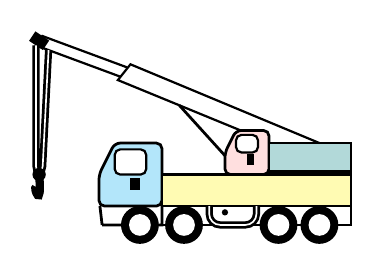
\begin{tikzpicture}[line width=1pt,scale=.4]
	% Vẽ phần cabin
	\filldraw[ cyan!30,rounded corners=2pt, draw=black] (0,0)--(0,1)--(0.5,2)--(2,2)--(2,0)--cycle; 
	%\draw(0.1,-0.6)--(0.2,-0.4)--(0.2,-0.4)--(2,-0.4)--(2,-0.6)--cycle;
	\draw[ line width=1pt] (0.1,-0.6)--(2,-0.6)--(2,0)(0.03,0)--(0.1,-0.6);
	% Cửa sổ cabin
	\filldraw[thick,rounded corners=2pt, white, draw=black] (0.5,1) rectangle (1.5,1.8); 
	\draw [line width=4pt](1,0.7)--(1.3,0.7);
	% Vẽ thân xe với các đường thẳng
	\filldraw[thick, yellow!30, draw=black] (2,0) -- (8,0) -- (8,1) -- (2,1) -- cycle;
	\draw (8,0)--(8,-0.6)--(2,-0.6);
	%thùng dầu
	\draw[double, rounded corners=4pt] (5,0)--(5,-0.6)--(3.5,-0.6)--(3.5,0);
	\fill(4,-0.2) circle(0.1);
	% Vẽ các bánh xe
	\foreach \x in {1.3,2.7, 5.7,7}
	\fill[black] (\x,-0.6) circle(0.6); % Bánh xe
	\foreach \x in {1.3,2.7, 5.7,7}
	\filldraw[white] (\x,-0.6) circle(0.3); % Bánh xe
	%cabin điều khiển cẩu
	\begin{scope}[shift={(4,1)}, scale=0.7]
	\filldraw[ rounded corners=2pt, pink!50, draw=black] (0,0)--(0,1)--(0.5,2)--(2,2)--(2,0)--cycle; 
	% Cửa sổ cabin
	\filldraw[thick,rounded corners=2pt,white, draw=black] (0.5,1) rectangle (1.5,1.8); 
	\draw [line width=4pt](1,0.7)--(1.3,0.7); 
	\end{scope}
	\filldraw[teal!30, draw=black](8,1.1)--(8,2)--(5.4,2)--(5.4,1.1)--cycle;
	% Vẽ cần cẩu
	\draw[thick] (4.5,2.4) -- (0.6,4) -- (1,4.5) -- (7,2);
	\draw[thick] (0.7,4.1)--(-2,5.1)--(-1.8,5.4)--(0.9,4.4);
	\draw[line width=6pt] (-2,5.1)--(-1.8,5.4);
	\draw(4,1.6)--(2.55,3.2);
	% Vẽ móc treo
	\draw[smooth,line width=3pt] (-1.9,1) .. controls ++(-85:1.2) and ++(-180:0.1) .. (-2,0.6);
	\draw[rounded corners=3pt, double] (-2,5.1)--(-2,1)--(-1.8,1)--(-1.6,4.95);
	\fill(-1.9,1) circle(6pt);
	\end{tikzpicture}
	}
	\shortans{$10,1$}
	\loigiai{
	\begin{tikzpicture}[scale=.6]
	\path
	(0,0) coordinate (K)
	(0,1) coordinate (D)
	(0,2) coordinate (A)
	(0,7) coordinate (B)
	(5,2) coordinate (C)
	(5,0) coordinate (H)
	;
	\draw (C)--(H) node [midway,right]{ $2{,}6$ m};
	\draw [dashed](K)--(H);
	\draw [<->] (-1,7)--(-1,1) node [midway,left] { $8{,}1$ m};
	\draw [<->](-1,1)--(-1,0) node [midway,left] { $1$ m};
	\draw (K)--(D)--++(0,1)--++(0,5)--++(5,-5)--++(0,-2) (C)--(A);
	\foreach \x/\g in {A/180,D/180,B/90,C/0,H/0,K/180}
	\fill[black](\x) circle (1pt) ( $(\x)+(\g:3mm)$ ) node{$\x$};
	\draw pic[draw,angle radius=2mm]{right angle=C--A--B};
	\draw pic[" $40^\circ$",draw=black,angle eccentricity=2,angle radius=.5cm,color=blue]{angle=B--C--A};
	\end{tikzpicture}\\
	\noindent
	Ta có tứ giác $AKHC$ là hình chữ nhật nên $AK=CH$. Suy ra $AD+DK=CH$ hay $AD=CH-DK=2{,}6-1=1{,}6$ m.\\
	$AB=BD-AD=8{,}1-1{,}6=6{,}5$ m.\\
	Xét $\triangle ABC$ vuông tại $A$, ta có \\
	$\sin{C}=\dfrac{AB}{BC}$\\
	Suy ra $BC=\dfrac{AB}{\sin{C}}=\dfrac{6{,}5}{\sin{40}^\circ}\approx 10{,}1$ m.\\
	Vậy cần cẩu phải dài $10{,}1$ m.
	}
\end{ex}
%%==========Câu 106
\begin{ex}%[9H4V1-5]
	%
	\immini[thm]
	{
	Giông bão thổi mạnh, một cây tre gãy gập xuống làm ngọn cây chạm đất và ngọn cây tạo với mặt đất một góc $30^\circ$. Người ta đo được khoảng cách từ chỗ ngọn cây chạm đất đến gốc cây tre là $8{,}5$ m. Giả sử cây tre mọc vuông góc với mặt đất, thì chiều cao của cây tre (làm tròn đến hàng phần mười) là $\ldots$
	}
	{
	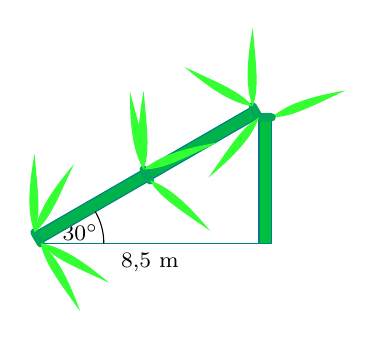
\begin{tikzpicture}[font=\footnotesize, line join=round, line cap=round, >=stealth,scale=0.4]
	\tikzset{la/.pic={
	\fill[green!80!white](0,0)..controls++(-20:0.5) and ++(-175:1)..(2,0)..controls++(170:1) and ++(20:0.5)..(0,0);
	}}
	\def\cao{4}
	\def\a{0.1*\cao}
	\pgfmathsetmacro{\dai}{\cao*sqrt(3)}
	\draw[fill=green!75!blue,draw=teal](0,0)rectangle(\a,\cao)pic[rotate=20,scale=0.5]{la};
	\draw[fill=green!70!blue,draw=teal](-\dai,0)--(0,\cao)coordinate(cao)--([turn]90:\a)--([turn]90:{2/sqrt(3)*\dai})--cycle;;
	\draw[teal](-\dai,0)coordinate(dai)--(0,0)coordinate(oo);
	\begin{scope}
	\clip(oo)--(cao)--(dai)--cycle;
	\draw(dai)circle(2)++(15:1.3)node{$30^\circ$};
	\end{scope}
	\draw[line width=3pt,green!65!blue](0,\cao)pic[rotate=-130,scale=0.5]{la}--(\a,\cao)(cao)--++(120:\a)pic[rotate=150,scale=0.5]{la}pic[rotate=90,scale=0.5]{la}(dai)--++(120:\a)(-0.5*\dai,0.5*\cao)pic[rotate=-40,scale=0.5]{la}--++(120:\a)pic[rotate=90,scale=0.5]{la}pic[rotate=20,scale=0.5]{la}pic[rotate=100,scale=0.5]{la};
	\path(dai)pic[rotate=-30,scale=0.5]{la}(dai)pic[rotate=-60,scale=0.5]{la}(dai)++(120:\a)pic[rotate=60,scale=0.5]{la}pic[rotate=90,scale=0.5]{la};
	\path(dai)--(oo)node[pos=0.5,below]{$8{,}5$ m};
	\end{tikzpicture}
	}
	\shortans{$14,7$}
	\loigiai{
	Xét $\triangle ACD$ vuông tại $C$, ta có \\
	$\tan\widehat{DCA}=\dfrac{AD}{AC}$
	$\Rightarrow AD=AC\cdot\tan\widehat{DCA}=8{,}5\cdot\tan{30}^\circ$\\
	$\cos\widehat{DCA}=\dfrac{AC}{DC}$
	$\Rightarrow DC=AC\cdot\cos\widehat{DCA}=8,5\cdot\cos{30}^\circ$\\
	$AB=AD+DC=8{,}5\cdot\tan{30}^\circ+\dfrac{8{,}5}{\cos{30}^\circ}\approx 14{,}72$ m.\\
	Vậy chiều cao của cây tre là $14{,}7$ m.
	}
\end{ex}
%%==========Câu 107
\begin{ex}%[9H4C1-5]
	%
	\immini[thm]
	{
	Hai chiếc tàu thủy cùng xuất phát từ một vị trí $A$ đi thẳng theo hai hướng tạo với nhau góc $60^\circ$. Tàu $B$ chạy với tốc độ $20$ hải lí một giờ. Tàu $C$ chạy với tốc độ $15$ hải lí một giờ. Sau hai giờ, khoảng cách giữa hai tàu (làm tròn đến hàng đơn vị) là $\ldots$
	}
	{
	\begin{tikzpicture}[scale=.45,font=\footnotesize]
	\path
	(-2,0) coordinate (A)
	(0,0) coordinate (H)
	(3,0) coordinate (B)
	(0,4) coordinate (C);
	\draw (A)--(C)(A)--(B);
	\foreach \x/\g in
	{A/180,B/120,C/90}
	\fill[black] (\x) circle (1pt)
	( $(\x)+(\g:3mm)$) node{$\x$};
	%\draw pic[draw,angle radius=2mm]{right angle=C--H--A};
	\draw pic[" $60^\circ$ ", draw=black, angle eccentricity=2, angle radius=.5cm, color=blue]
	{angle=B--A--C}; 
	\tikzset{Icon-Tau/.pic={
	\fill[ball color=brown!80!cyan!80!white](-4.65,0.08)..controls+(-23:2.5) and+(-165:3.5)..(4.6,0)..controls+(15:0.15) and+(-15:0.5)..(3.9,0.2)..controls+(-172:5) and+(15:2)..(-4.65,0.08);
	%%Thành trong tầu
	\fill[ball color=gray!10!cyan] [red](-4.65,0.08)--+(-25:0.4)..controls+(10:2) and++(-172:5)..(3.8,0)--++(110:0.2)..controls+(-172:5) and+(15:2)..(-4.65,0.08);
	%%Trung tâm tàu
	\fill[ball color=gray!20](-0.25,-0.42)--++(48:1)coordinate(x)--++(-5:0.85)coordinate(y)--++(-112:1.1)coordinate(z)--cycle;
	\fill[ball color=gray!10](x)--(y)--++(0:0.5)coordinate(t)--++(170:1)coordinate(u)--++(180:0.2)--cycle;
	\fill[cyan](t)--++(72:0.7)coordinate(a)--++(175:0.85)coordinate(b)--(u)--cycle;
	\fill[ball color=gray!20!green](a)--++(2:1.2)coordinate(c)--++(165:0.6)--++(-178:1.25)--(b)--cycle;
	\fill[ball color=gray!20](z)--(y)--(t)--(a)--(c)--++(-70:0.4)coordinate(d)--++(2:0.5)coordinate(e)--++(-80:1)--cycle ($(d)!0.5!(c)$)coordinate(m);
	\fill[ball color=gray!20,draw=gray](d)--(e)--(m)--cycle;
	%%Hét trung tâm tàu
	\fill[ball color=gray!90!cyan](-4.65,0.08)..controls+(-23:2.5) and+(-165:3.5)..(4.6,0)..controls+(15:0.05) and++(65:1.2)..(4.2,-1)..controls++(-152:0.75) and+(13:2)..(-1,-2.5)..controls++(-167:1.1) and+(-50:3.5)..(-4.65,0.08);
	\fill[ball color=gray!30!white](2,1.5)--++(80:2)arc(-95:-450:1 and 0.1)--++(-92:2)--cycle;
	\fill[ball color=gray!90!cyan](2,1)coordinate(e)--++(0:0.4)--++(88:0.65)--++(175:0.3)coordinate(f)--cycle;
	\fill[ball color=gray!90!cyan](e)--(f)--++(180:0.2)--++(-115:0.7)--cycle;
	\clip (-4.65,0.08)..controls+(-23:2.5) and+(-165:3.5)..(4.6,0)..controls+(15:0.05) and++(65:1.2)..(4.2,-1)..controls++(-152:0.75) and+(13:2)..(-1,-2.5)..controls++(-167:1.1) and+(-50:3.5)..(-4.65,0.08);
	\fill[red](-4,-0.7)..controls++(-30:2) and++(-160:3)..(4.5,-0.3)--++(-90:0.25)..controls++(-160:3) and++(-25:1.5)..(-3.6,-1.1);
	}}
	\path(C)pic[scale=.12]{Icon-Tau};
	\path(B)pic[scale=.12]{Icon-Tau};
	\end{tikzpicture}
	}
	\shortans{$36$}
	\loigiai{
	\begin{center}
	\begin{tikzpicture}[scale=.6]
	\path
	(-2,0) coordinate (A)
	(0,0) coordinate (H)
	(3,0) coordinate (B)
	(0,4) coordinate (C);
	\draw (A)--(C)(A)--(B);
	\foreach \x/\g in
	{A/180,B/120,C/90}
	\fill[black] (\x) circle (1pt)
	( $(\x)+(\g:3mm)$) node{$\x$};
	%\draw pic[draw,angle radius=2mm]{right angle=C--H--A};
	\draw pic[" $60^\circ$ ", draw=black, angle eccentricity=2, angle radius=.5cm, color=blue]
	{angle=B--A--C}; 
	\tikzset{Icon-Tau/.pic={
	\fill[ball color=brown!80!cyan!80!white](-4.65,0.08)..controls+(-23:2.5) and+(-165:3.5)..(4.6,0)..controls+(15:0.15) and+(-15:0.5)..(3.9,0.2)..controls+(-172:5) and+(15:2)..(-4.65,0.08);
	%%Thành trong tầu
	\fill[ball color=gray!10!cyan] [red](-4.65,0.08)--+(-25:0.4)..controls+(10:2) and++(-172:5)..(3.8,0)--++(110:0.2)..controls+(-172:5) and+(15:2)..(-4.65,0.08);
	%%Trung tâm tàu
	\fill[ball color=gray!20](-0.25,-0.42)--++(48:1)coordinate(x)--++(-5:0.85)coordinate(y)--++(-112:1.1)coordinate(z)--cycle;
	\fill[ball color=gray!10](x)--(y)--++(0:0.5)coordinate(t)--++(170:1)coordinate(u)--++(180:0.2)--cycle;
	\fill[cyan](t)--++(72:0.7)coordinate(a)--++(175:0.85)coordinate(b)--(u)--cycle;
	\fill[ball color=gray!20!green](a)--++(2:1.2)coordinate(c)--++(165:0.6)--++(-178:1.25)--(b)--cycle;
	\fill[ball color=gray!20](z)--(y)--(t)--(a)--(c)--++(-70:0.4)coordinate(d)--++(2:0.5)coordinate(e)--++(-80:1)--cycle ($(d)!0.5!(c)$)coordinate(m);
	\fill[ball color=gray!20,draw=gray](d)--(e)--(m)--cycle;
	%%Hét trung tâm tàu
	\fill[ball color=gray!90!cyan](-4.65,0.08)..controls+(-23:2.5) and+(-165:3.5)..(4.6,0)..controls+(15:0.05) and++(65:1.2)..(4.2,-1)..controls++(-152:0.75) and+(13:2)..(-1,-2.5)..controls++(-167:1.1) and+(-50:3.5)..(-4.65,0.08);
	\fill[ball color=gray!30!white](2,1.5)--++(80:2)arc(-95:-450:1 and 0.1)--++(-92:2)--cycle;
	\fill[ball color=gray!90!cyan](2,1)coordinate(e)--++(0:0.4)--++(88:0.65)--++(175:0.3)coordinate(f)--cycle;
	\fill[ball color=gray!90!cyan](e)--(f)--++(180:0.2)--++(-115:0.7)--cycle;
	\clip (-4.65,0.08)..controls+(-23:2.5) and+(-165:3.5)..(4.6,0)..controls+(15:0.05) and++(65:1.2)..(4.2,-1)..controls++(-152:0.75) and+(13:2)..(-1,-2.5)..controls++(-167:1.1) and+(-50:3.5)..(-4.65,0.08);
	\fill[red](-4,-0.7)..controls++(-30:2) and++(-160:3)..(4.5,-0.3)--++(-90:0.25)..controls++(-160:3) and++(-25:1.5)..(-3.6,-1.1);
	}}
	\path(C)pic[scale=.2]{Icon-Tau};
	\path(B)pic[scale=.2]{Icon-Tau};
	\end{tikzpicture}
	\begin{tikzpicture}[scale=.6]
	\path
	(-2,0) coordinate (A)
	(0,0) coordinate (H)
	(3,0) coordinate (B)
	(0,4) coordinate (C);
	\draw (A)--(H)--++(3,0)--++(-3,4)--cycle (C)--(H);
	\foreach \x/\g in
	{A/180,H/-90,B/0,C/90}
	\fill[black] (\x) circle (1pt)
	( $(\x)+(\g:3mm)$) node{$\x$};
	\draw pic[draw,angle radius=2mm]{right angle=C--H--A};
	\draw pic[" $60^\circ$ ", draw=black, angle eccentricity=2, angle radius=.5cm, color=blue]
	{angle=B--A--C}; 
	\end{tikzpicture}
	\end{center}
	Sau $2$ giờ:\\
	Tàu $B$ đi được: $AB=20\cdot 2=40$ hải lí.\\
	Tàu $C$ đi được: $AC=15\cdot 2=30$ hải lí.\\
	Vậy tam giác $ABC$ có $AB=40$, $AC=30$ và $\widehat{A}=60^\circ$. \\ 
	Kẻ $CH \perp AB$ tại $H$, $\triangle AHC$ vuông tại $H$, ta có
	$AH=AC \cdot \cos A=30 \cdot \cos 60^\circ=15$ hải lí.\\
	$CH=AC \cdot \sin A=30 \cdot \sin 60^\circ\approx 26$ hải lí.\\
	$HB=AB-AH=40-15=25$ hải lí.\\
	Xét $\triangle BHC$ vuông tại $H$, ta có \\ 
	$BC^2=CH^2+BH^2=26^2+25^2=1301$.\\
	Vậy $BC=\sqrt{1301}\approx 36$ hải lí.
	}
\end{ex}
%%==========Câu 108
\begin{ex}%[9H4C1-5]
	%
	Để xác định khoảng cách từ một gốc cây $A$ trên một hòn đảo nhỏ giữa biển đến vị trí con sao biển $C$ trên bãi cát, người ta chọn một điểm $B$ trên bãi biển cách điểm $C$ một khoảng $1\,225$ m và dùng giác kế ngắm xác định được $\widehat{ABC}=75^\circ$; $\widehat{ACB}=65^\circ$. Khi đó, khoảng cách từ gốc cây $A$ trên hòn đảo đến con sao biển $C$ trên bãi cát là $\ldots$ mét (kết quả làm tròn đến đơn vị mét).
	%	\begin{center}
	%	\begin{tikzpicture}[scale=.7,font=\footnotesize]
	%	% Mặt biển
	%	\fill[top color=white, bottom color=cyan!70] (0,3) rectangle (10,0); % Mặt biển với màu xanh nhạt
	%	% Bờ biển với đường cong
	%	\fill[cyan!80!blue!70] (0,0) .. controls (2,0.5) and (4,0.3) .. (10,0) -- (10,-2) -- (0,-1) -- cycle;
	%	\fill[yellow!80!orange!50] (0,-1) .. controls (8,0) and (8,-1.8) .. (10,-0.3) -- (10,-3) -- (0,-3) -- cycle;
	%	\fill[brown!30] (2,0.3) .. controls (6,1) and (5,2) .. (8,0.1) -- (4,0.3) -- cycle;
	%	\fill[green] (3,0.4) .. controls (3,0) and (3,2) .. (7,0.3) -- (4,0.3) -- cycle;
	%	%\path (3.5,1.2)node[scale=10]{\twemoji{1f3dd}};
	%	\path (5,1.2)node[scale=2]{\twemoji{1f335}};
	%	\path (7,1)node[scale=4]{\twemoji{1f335}};
	%	\path (6,1)node[scale=7]{\twemoji{1f334}};
	%	\path (3.5,1.3)node[scale=9]{\twemoji{1f334}};
	%	\begin{scope}[shift={(6.7,-1.5)}, scale=0.2, rotate=20]
	%	\pgfmathsetmacro{\ct}{3} 
	%	\pgfmathsetmacro{\cc}{\ct*sin(18)/sin(126)} 
	%	% star
	%	\filldraw[ultra thick, rounded corners=4pt, red] (0,0)
	%	+(90-0*36:\ct) coordinate(T1)
	%	foreach[evaluate=\x as \nc using int((\x+1)/2), 
	%	evaluate=\x as \nt using int((\x+1)/2+1)] 
	%	\x in {1,3,...,9}{
	%	-- +(90-\x*36:\cc) coordinate(C\nc) -- +({90-(\x+1)*36}:\ct) coordinate(T\nt)}
	%	-- cycle;
	%	\end{scope}
	%	\begin{scope}[shift={(3,-2.2)}, scale=0.53, rotate=-10]
	%	\path
	%	(0,5) coordinate (A)
	%	(2,1) coordinate (H)
	%	(3,-1) coordinate (B)
	%	(6,3) coordinate (C);
	%	\draw (B)--(C) node [midway,below,sloped]{ $1225$ m};
	%	\draw (A)--(H)--++(1,-2)--++(3,4)--cycle ;
	%	\foreach \x/\g in {A/180,B/-90,C/120}
	%	\fill[black] (\x) circle (1pt)
	%	( $(\x)+(\g:6mm)$) node{$\x$};
	%	%\draw pic[draw,angle radius=2mm]{right angle=C--H--A};
	%	\draw pic[" $75^\circ$ ",draw=black, angle eccentricity=1.2, angle radius=.5cm, color=blue]
	%	{angle=C--B--A}; 
	%	\draw pic[" $65^\circ$ ",draw=black, angle eccentricity=1.2, angle radius=.5cm, color=blue]
	%	{angle=A--C--B}; 
	%	\end{scope}
	%	\end{tikzpicture}
	%	\end{center}
	\shortans{$1840$}
	\loigiai{
	\begin{center}
	\begin{tikzpicture}[scale=.5]
	\path
	(0,5) coordinate (A)
	(2,1) coordinate (H)
	(3,-1) coordinate (B)
	(6,3) coordinate (C);
	\draw (B)--(C) node [midway,below,sloped]{ $1225$ m};
	\draw (A)--(H)--++(1,-2)--++(3,4)--cycle (C)--(H);
	\foreach \x/\g in {A/180,H/180,B/0,C/0}
	\fill[black] (\x) circle (1pt)
	( $(\x)+(\g:6mm)$) node{$\x$};
	\draw pic[draw,angle radius=2mm]{right angle=C--H--A};
	\draw pic[" $75^\circ$ ",draw=black, angle eccentricity=2, angle radius=.5cm, color=blue]
	{angle=C--B--A}; 
	\draw pic[" $65^\circ$ ",draw=black, angle eccentricity=2, angle radius=.5cm, color=blue]
	{angle=A--C--B}; 
	\end{tikzpicture}
	\end{center}
	Xét $\triangle ABC$ có $\widehat{ABC}=75^\circ$ và $\widehat{ACB}=65^\circ$ nên ta có \\
	$\widehat{BAC}=180^\circ - \left(\widehat{ABC} + \widehat{ACB}\right) = 180^\circ - \left(75^\circ + 65^\circ\right) = 40^\circ$. \\
	Kẻ $CH \perp AB$ tại $H$, xét $\triangle BCH$ vuông tại $H$, ta có \\
	$BH = BC \cdot \cos B = 1225 \cdot \cos 75^\circ \approx 317$ m. \\ 
	$CH = BC \cdot \sin B = 1225 \cdot \sin 75^\circ \approx 1183$ m. \\
	Xét $\triangle ACH$ vuông tại $H$, ta có \\
	$AC = \dfrac{CH}{\sin A} = \dfrac{1183}{\sin 40^\circ} \approx 1840$ m. \\
	Vậy khoảng cách từ một gốc cây $A$ trên hòn đảo đến con sao biển $C$ trên bãi cát là $1840$ m.
	}
\end{ex}
%%==========Câu 109
\begin{ex}%[9H4C1-5]
	%
	\immini[thm]
	{
	Một chiếc cầu trượt bao gồm phần cầu thang (để bước lên) và phần ống trượt (để trượt xuống) nối liền với nhau. Khi xây dựng, cần thiết kế phần ống trượt nghiêng với mặt đất một góc là $50^\circ$ và phần cầu thang cũng đặt nghiêng. Nếu độ dài ống trượt là $3$ m, phần cầu thang bước lên có độ dài $2{,}5$ m thì khoảng cách từ chân cầu thang đến chân ống trượt (làm tròn kết quả đến hàng phần mười) là$\ldots$
	}
	{	\begin{tikzpicture}[line join=round, line cap=round,>=stealth,thick,scale=.35,font=\footnotesize]
	\path (-4,0.5) coordinate (C)--(-2.5,0) coordinate (D)--(0,3) coordinate (A) --(-1.5,3.5) coordinate (B)--cycle;
	\coordinate (x1) at (-0.001,0);
	\coordinate (x2) at (0.001,0);
	\coordinate (A1) at ($(A)+(2.4,0)$);
	\coordinate (B1) at ($(B)+(2.4,0)$);
	\coordinate (A2) at ([scale around={0.3:(A)}] A1);
	\coordinate (A3) at ([scale around={0.5:(A)}] A1);
	\coordinate (H2) at ($(x1)!(A2)!(x2)$);
	\coordinate (H3) at ($(x1)!(A3)!(x2)$);
	\coordinate (E) at (2,0.5);
	\coordinate (F) at ($(A1)+(E)-(B1)$);
	\draw[line width = 2, brown] (A1)--(F)--(E)--(B1)--cycle;
	\foreach \i in {0.1, 0.2, ..., 0.9} {\draw[line width = 2, red] ($(A1)!\i!(F)$)--($(B1)!\i!(E)$);}
	\draw[line width=2,brown,fill=black!20](A2)--(A3)--(H3)--(H2)--cycle;
	\coordinate (B2) at ([scale around={0.3:(B)}] B1);
	\coordinate (B3) at ([scale around={0.5:(B)}] B1);
	\coordinate (K2) at ($(B2)+(H2)-(A2)$);
	\coordinate (K3) at ($(B3)+(H3)-(A3)$);
	\draw[line width=2,brown,fill=black!20](B2)--(B3)--(K3)--(K2)--cycle;
	%\fill[yellow!10] ($(D)+(0.2,0)$)--($(A)+(0.2,0)$)--($(B)+(0.2,0)$)--($(C)+(0.2,0)$)--cycle;
	%\draw[brown, line width = 2] ($(A)+(0.2,0)$)--($(D)+(0.2,0)$)--(D);
	\draw[line width = 2, brown, fill=yellow!10] (A)--(B)--(C)--(D)--cycle;
	\fill[black!50] (A)--(B)--(B1)--(A1)--cycle;
	\draw[line width = 2, brown] (A)--(A1) (B)--(B1);
	\draw[line width = 2, brown, fill=green!15] ($(B)$) arc (180:0:1.2 cm and 1 cm);
	\path[pattern=vertical lines] (B) arc (180:0:1.2 cm and 1 cm);
	\draw[line width = 2, brown, fill=green!15] ($(A)$) arc (180:0:1.2 cm and 1 cm);
	\coordinate (C1) at ($(C)!0.15!(B)$); 
	\coordinate (D1) at ($(D)!0.15!(A)$); 
	%\coordinate (B4) at ($(B)!0.15!(C)$); 
	%\coordinate (A4) at ($(A)!0.15!(D)$); 
	\fill[yellow!10] ($(C)+(-0.5,0)$)--(C)--(D)--($(D)+(-0.5,0)$)--cycle;
	\draw[line width = 2,brown] ($(C)+(-0.5,0)$)--($(D)+(-0.5,0)$);
	%\fill[violet!30] (A4)--($(A4)+(-0.5,0)$) .. controls +(90:0.55) and +(180:0.55) .. (A);
	%\draw[line width = 2,brown] ($(A4)+(-0.5,0)$) .. controls +(90:0.55) and +(180:0.55) .. (A);
	\draw[line width = 2,brown,fill = violet!30] (C)--(C1) .. controls +(180:0.55) and +(90:0.5) .. ($(C)+(-0.5,0)$) coordinate [pos = 0.3] (C2) -- (C);
	\draw[line width = 2,brown,fill = violet!30] (D)--(D1) .. controls +(180:0.55) and +(90:0.55) .. ($(D)+(-0.5,0)$) coordinate [pos = 0.3] (D2) -- (D);
	\draw[line width = 2,brown,fill = violet!30] (C2) .. controls +(50:3) and +(180:0.5) .. (B)--(C1);
	\draw[line width = 2,brown,fill = violet!30] (D2) .. controls +(50:3) and +(180:0.5) .. (A)--(D1);
	\path[pattern=vertical lines] (A) arc (180:0:1.2 cm and 1 cm);
	\end{tikzpicture}
	\begin{tikzpicture}[xscale=-1,scale=.5,font=\footnotesize]
	\path
	(-2,0) coordinate (A)
	(0,0) coordinate (H)
	(3,0) coordinate (B)
	(0,5) coordinate (C)
	;
	\draw (A)--(C) node [midway, right]{$2{,}5$ m};
	\draw (B)--(C) node [midway,left]{$ 3 $ m};
	\draw (A)--(H)--++(3,0)--++(-3,5)--cycle (C)--(H);
	\foreach \x/\g in
	{A/180,H/-90,B/0,C/90}
	\fill[black](\x) circle (1pt)
	($ (\x)+(\g:6mm) $) node{$\x$};
	\draw pic[draw,angle radius=2mm]{right angle=C--H--A};
	\draw pic["$50^\circ $",draw=black, angle eccentricity=2, angle radius=.5cm, color=blue]
	{angle=A--B--C}; 
	\end{tikzpicture}
	}
	\shortans{$2,9$}
	\loigiai{
	Ta có \\
	$BC=3$ m là độ dài ống trượt.\\
	$AC=2{,}5$ m là độ dài phần cầu thang bước lên.\\
	$\widehat{B}=50^\circ$ là góc tạo bời phần ống trượt với mặt đất.\\
	\begin{itemize}
	\item Xét $\triangle CBH$ vuông tại $H$, áp dụng hệ thức giữa cạnh và góc nhọn trong tam giác vuông ta có:
	\[
	\widehat{CBH}=\dfrac{BH}{BC} \quad\text{suy ra}\quad BH=BC\cdot \cos\widehat{CBH}=3\cdot\cos 50^\circ.
	\]
	\[\sin \widehat{C B H}=\dfrac{CH}{BC}\quad\text{suy ra}\quad CH=BC \cdot \sin \widehat{CBH}=3 \cdot \sin 50^\circ.\]
	\item Xét $\triangle CAH$ vuông tại $H$, áp dụng định lý Pythagore ta có\\
	\[A H^2=A C^2-C H^2=2{,}5^2-\left(3 \cdot \sin 50^{\circ}\right)^2 \quad\text{suy ra}\quad A H=\sqrt{2{,}5^2-\left(3 \cdot \sin 50^\circ\right)^2}\]
	\end{itemize}
	Ta có $AB=AH+BH \quad\text{suy ra}\quad AB=\sqrt{2{,}5^2-\left(3 \cdot \sin 50^\circ\right)^2}+3 \cdot \cos 50^\circ \approx 2{,}9$ m.\\
	Vậy khoảng cách từ chân cầu thang đến chân ống trượt khoảng $2{,}9$ m.
	}
\end{ex}
%%==========Câu 110
\begin{ex}%[9H4C1-5]
	%
	\immini[thm]
	{
	Cầu Cần Thơ là cây cầu dây văng có nhịp chính dài nhất khu vực Đông Nam Á. Biết tại hai điểm (ở cùng một phía so với cầu) cách nhau $89$ m trên mặt sông người ta nhìn thấy đỉnh trụ cầu với góc nâng lần lượt là $40^\circ$ và $30^\circ$. Chiều cao của trụ cầu Cần thơ so với mặt sông Hậu (làm tròn đến hàng đơn vị) là $\ldots$.
	}
	{
	\begin{tikzpicture}[rotate=.8,scale=.4]
	% Mặt cầu
	\draw[thick] (-7,0) -- (7,0);
	% Trụ tháp bên trái
	\fill[pink] (-4.5,0) -- (-4,5) -- (-3.5,0) -- cycle; % tô màu cho trụ bên ngoài
	\draw[thick] (-4.5,0) -- (-4,5) -- (-3.5,0); % khung ngoài trụ
	\fill[white] (-4.2,0) -- (-4,4.5) -- (-3.8,0) -- cycle; % tô màu cho trụ bên trong
	\draw[thick] (-4.2,0) -- (-4,4.5) -- (-3.8,0); % khung bên trong trụ
	\draw[thick, double] (-4.2,2.5) -- (-3.8,2.5); % thanh ngang ở giữa trụ
	% Trụ tháp bên phải 
	\fill[pink] (4.5,0) -- (4,5) -- (3.5,0) -- cycle; % tô màu cho trụ bên ngoài
	\draw[thick] (4.5,0) -- (4,5) -- (3.5,0); % khung ngoài trụ
	\fill[white] (4.2,0) -- (4,4.5) -- (3.8,0) -- cycle; % tô màu cho trụ bên trong
	\draw[thick] (4.2,0) -- (4,4.5) -- (3.8,0); % khung bên trong trụ
	\draw[thick, double] (4.2,2.5) -- (3.8,2.5); % thanh ngang ở giữa trụ
	% Dây văng trái 
	\draw[thin, blue] (-4,5) -- (-7,0); % dây trái ngoài cùng
	\draw[thin, blue] (-4,5) -- (-6,0);
	\draw[thin, blue] (-4,5) -- (-5,0);
	\draw[thin, blue] (-4,5) -- (-4,0);
	\draw[thin, blue] (-4,5) -- (-3,0);
	\draw[thin, blue] (-4,5) -- (-2,0);
	\draw[thin, blue] (-4,5) -- (-1,0);
	% Dây văng phải 
	\draw[thin, blue] (4,5) -- (7,0); % dây phải ngoài cùng
	\draw[thin, blue] (4,5) -- (6,0);
	\draw[thin, blue] (4,5) -- (5,0);
	\draw[thin, blue] (4,5) -- (4,0);
	\draw[thin, blue] (4,5) -- (3,0);
	\draw[thin, blue] (4,5) -- (2,0);
	\draw[thin, blue] (4,5) -- (1,0);
	% Mặt đất dưới cầu
	\draw[thick] (-7,-0.2) -- (7,-0.2);
	% Phần móng trụ cầu
	\fill[gray!80] (-4.7,-0.2) rectangle (-3.3,-1); % móng trụ trái
	\fill[gray!80] (4.7,-0.2) rectangle (3.3,-1); % móng trụ phải
	\fill[top color=white, middle color=cyan!60,white] (-7,-0.6) rectangle (7,-1.7); % mặt nước
	\end{tikzpicture}
	}
	\shortans{$165$}
	\loigiai{
	\begin{center}
	\begin{tikzpicture}[scale=.6]
	\path
	(0,0) coordinate (A)
	(5,0) coordinate (D)
	(7,0) coordinate (C)
	(0,5) coordinate (B)
	;
	%	\draw (A)--(C) node [midway,above,sloped]{$ 2{,}5 $m};
	%	\draw (B)--(C) node [midway,above,sloped]{$ 3 $m};
	\draw (A)--(D)--++(2,0)--++(-7,5)--cycle (B)--(D);
	\foreach \x/\g in
	{A/180,D/-90,B/90,C/0}
	\fill[black](\x) circle (1pt)
	($ (\x)+(\g:6mm) $) node{$\x$};
	\draw pic[draw,angle radius=2mm]{right angle=C--H--A};
	\draw pic["$30^\circ $",draw=black, angle eccentricity=2, angle radius=.5cm, color=blue]
	{angle=B--C--A}; \draw pic["$40^\circ $",draw=black, angle eccentricity=2, angle radius=.5cm, color=blue]
	{angle=B--D--A}; 
	\end{tikzpicture}
	\end{center}
	$AB$ là chiều cao của cầu $D$,\\ 
	$C$ là hai vị trí trên sông cách nhau $89$ m, tức là $DC = 89$ m.\\ 
	Khi đó $\widehat{BDA} = 40^\circ$, $\widehat{BCA} = 30^\circ$.\\
	Xét $\triangle ABD$ vuông tại $A$, ta có 
	\[
	\tan \widehat{ADB} = \dfrac{AB}{AD} \Rightarrow AD = \dfrac{AB}{\tan \widehat{ADB}} = \dfrac{AB}{\tan 40^\circ}.
	\] 
	Xét $\triangle ABC$ vuông tại $A$, ta có
	\[
	\tan \widehat{ACB} = \dfrac{AB}{AC} \Rightarrow AC = \dfrac{AB}{\tan \widehat{ACB}} = \dfrac{AB}{\tan 30^\circ}.
	\] 
	Ta có
	\[
	DC = AC - AD = \dfrac{AB}{\tan 30^\circ} - \dfrac{AB}{\tan 40^\circ} = AB\left(\dfrac{1}{\tan 30^\circ} - \dfrac{1}{\tan 40^\circ}\right).
	\] 
	Suy ra 
	\[
	AB = \dfrac{DC}{\dfrac{1}{\tan 30^\circ} - \dfrac{1}{\tan 40^\circ}} = \dfrac{89}{\dfrac{1}{\tan 30^\circ} - \dfrac{1}{\tan 40^\circ}} \approx 165\left(\mathrm{m}\right) .
	\]
	Vậy chiều cao của trụ cầu Cần Thơ so với mặt sông Hậu là $165$ m.
	}
\end{ex}
%%==========Câu 111
\begin{ex}%[9H4C1-5]
	%
	\immini[thm]
	{
	Hai chiếc khinh khí cầu cùng được thả lên từ một độ cao $350$ m (ở hai vị trí $A$ và $B$). Tại một điểm $C$ ở mặt đất, người ta quan sát và đo các góc, kết quả được minh họa như hình vẽ. Khoảng cách $AB$ giữa hai chiếc khinh khí cầu (làm tròn kết quả đến mét) là $\ldots$
	}
	{
	\begin{tikzpicture}[scale=.35]
	\path
	(-5,0) coordinate (C)
	(0,0) coordinate (H)
	(2,0) coordinate (I)
	(2,6) coordinate (B)
	(0,6) coordinate (A);
	\draw (B)--(I) node [midway,right]{ $350$ m};
	\draw (C)--(H)--++(2,0)--++(0,6)--++(-2,0)--cycle (A)--(H) (C)--(B);
	\foreach \x/\g in
	{A/90,I/-0,B/90,C/-90,H/-90}
	\fill[black](\x) circle (1pt)
	( $(\x)+(\g:1.1cm)$ node{$\x$});
	\draw pic[draw,angle radius=2mm]{right angle=C--H--A};
	\draw pic[draw,angle radius=2mm]{right angle=C--I--B};
	\draw pic[" $40^\circ$ ",draw=black, angle eccentricity=2, angle radius=.5cm, color=blue]
	{angle=H--C--B}; 
	\foreach \x/\y in {A/180,B/0,C/-90,H/-90,I/-90}{\fill (\x) circle(1pt) ($(\x)+(\y:0.8cm)$)node{$\x$};}
	\begin{scope}[shift={(0,7.3)}, scale=0.4]
	\begin{scope}
	\clip (-2.2,-.1) rectangle (2.2,5.4);
	\fill[blue!30!black,draw] (-.5,0) coordinate(A) .. controls ++(100:.1) and ++(-70:.2) .. (-.7,.7) coordinate(B) -- (.7,.7) coordinate(C) .. controls ++(-110:.2) and ++(80:.1) .. (.5,0) coordinate(D) -- cycle;
	\shade[ball color=blue!60] (B) .. controls ++(130:8) and ++(50:8) .. (C);
	\clip (B) .. controls ++(130:8) and ++(50:8) .. (C) -- cycle;
	\shade[ball color=white] (.2,0) .. controls ++(50:1) and ++(-15:3) .. (0,5.5) .. controls ++(-60:2.5) and ++(80:1) .. cycle
	(-.2,0) .. controls ++(130:1) and ++(195:3) .. (0,5.5) .. controls ++(-120:2.5) and ++(100:1) .. cycle;
	\end{scope}
	\draw (A)--++(-75:.5) coordinate(E) -- ($(A)!(E)!(D)$) (D)--++(-105:.5) coordinate(F) -- ($(A)!(F)!(D)$);
	\tikzset{tui/.pic={
	\fill[brown!60!black] (0:.1) arc (0:360:.1cm and .2cm);
	}}
	\begin{scope}
	\clip[rounded corners] ([shift={(-.2,.25)}]E) -- ([shift={(.2,.25)}]F) -- ++(-90:1.3) coordinate(G)--([shift={(-.4,0)}]$(E)+(G)-(F)$) coordinate(H) --cycle;
	\fill[white,draw=black, rounded corners] ([shift={(-.2,.25)}]E) -- ([shift={(.2,.25)}]F) -- ++(-90:1.5) coordinate(G)--([shift={(-.4,0)}]$(E)+(G)-(F)$) coordinate(H) --cycle;
	\fill[brown] (H) rectangle ([shift={(.2,.25)}]$(F)!.4!(G)$);
	\end{scope}
	\path (-.6,-1) pic[xslant=.2]{tui} (0,-1) pic{tui} (.6,-1) pic[xslant=-.2]{tui};
	\fill[brown,draw=black,rounded corners] (-.75,-.9) rectangle (.75,-.6);
	\end{scope}
	\begin{scope}[shift={(2,7.3)}, scale=0.4]
	\begin{scope}
	\clip (-2.2,-.1) rectangle (2.2,5.4);
	\fill[blue!30!black,draw] (-.5,0) coordinate(A) .. controls ++(100:.1) and ++(-70:.2) .. (-.7,.7) coordinate(B) -- (.7,.7) coordinate(C) .. controls ++(-110:.2) and ++(80:.1) .. (.5,0) coordinate(D) -- cycle;
	\shade[ball color=red!60] (B) .. controls ++(130:8) and ++(50:8) .. (C);
	\clip (B) .. controls ++(130:8) and ++(50:8) .. (C) -- cycle;
	\shade[ball color=white] (.2,0) .. controls ++(50:1) and ++(-15:3) .. (0,5.5) .. controls ++(-60:2.5) and ++(80:1) .. cycle
	(-.2,0) .. controls ++(130:1) and ++(195:3) .. (0,5.5) .. controls ++(-120:2.5) and ++(100:1) .. cycle;
	\end{scope}
	\draw (A)--++(-75:.5) coordinate(E) -- ($(A)!(E)!(D)$) (D)--++(-105:.5) coordinate(F) -- ($(A)!(F)!(D)$);
	\tikzset{tui/.pic={
	\fill[brown!60!black] (0:.1) arc (0:360:.1cm and .2cm);
	}}
	\begin{scope}
	\clip[rounded corners] ([shift={(-.2,.25)}]E) -- ([shift={(.2,.25)}]F) -- ++(-90:1.3) coordinate(G)--([shift={(-.4,0)}]$(E)+(G)-(F)$) coordinate(H) --cycle;
	\fill[white,draw=black, rounded corners] ([shift={(-.2,.25)}]E) -- ([shift={(.2,.25)}]F) -- ++(-90:1.5) coordinate(G)--([shift={(-.4,0)}]$(E)+(G)-(F)$) coordinate(H) --cycle;
	\fill[brown] (H) rectangle ([shift={(.2,.25)}]$(F)!.4!(G)$);
	\end{scope}
	\path (-.6,-1) pic[xslant=.2,scale=.8]{tui} (0,-1) pic[scale=.8]{tui} (.6,-1) pic[xslant=-.2]{tui};
	\fill[brown,draw=black,rounded corners] (-.75,-.9) rectangle (.75,-.6);
	\end{scope}
	\end{tikzpicture}
	}
	\shortans{$123$}
	\loigiai{
	\begin{center}
	\begin{tikzpicture}[scale=.6]
	\path
	(-5,0) coordinate (C)
	(0,0) coordinate (H)
	(2,0) coordinate (I)
	(2,6) coordinate (B)
	(0,6) coordinate (A);
	\draw (B)--(I) node [midway,right]{ $350$ m};
	\draw (C)--(H)--++(2,0)--++(0,6)--++(-2,0)--cycle (A)--(H) (C)--(B);
	\foreach \x/\g in
	{A/90,I/0,B/90,C/180,H/-90}
	\fill[black](\x) circle (1pt)
	( $(\x)+(\g:6mm)$ node{$\x$});
	\draw pic[draw,angle radius=2mm]{right angle=C--H--A};
	\draw pic[draw,angle radius=2mm]{right angle=C--I--B};
	\draw pic[" $40^\circ$ ",draw=black, angle eccentricity=2, angle radius=.5cm, color=blue]
	{angle=H--C--B}; 
	\foreach \x/\y in {A/90,B/90,C/-90,H/-90,I/-90}{\fill (\x) circle(1pt) ($(\x)+(\y:0.8cm)$)node{$\x$};}
	\begin{scope}[shift={(0,7.3)}, scale=0.4]
	\begin{scope}
	\clip (-2.2,-.1) rectangle (2.2,5.4);
	\fill[blue!30!black,draw] (-.5,0) coordinate(A) .. controls ++(100:.1) and ++(-70:.2) .. (-.7,.7) coordinate(B) -- (.7,.7) coordinate(C) .. controls ++(-110:.2) and ++(80:.1) .. (.5,0) coordinate(D) -- cycle;
	\shade[ball color=blue!60] (B) .. controls ++(130:8) and ++(50:8) .. (C);
	\clip (B) .. controls ++(130:8) and ++(50:8) .. (C) -- cycle;
	\shade[ball color=white] (.2,0) .. controls ++(50:1) and ++(-15:3) .. (0,5.5) .. controls ++(-60:2.5) and ++(80:1) .. cycle
	(-.2,0) .. controls ++(130:1) and ++(195:3) .. (0,5.5) .. controls ++(-120:2.5) and ++(100:1) .. cycle;
	\end{scope}
	\draw (A)--++(-75:.5) coordinate(E) -- ($(A)!(E)!(D)$) (D)--++(-105:.5) coordinate(F) -- ($(A)!(F)!(D)$);
	\tikzset{tui/.pic={
	\fill[brown!60!black] (0:.1) arc (0:360:.1cm and .2cm);
	}}
	\begin{scope}
	\clip[rounded corners] ([shift={(-.2,.25)}]E) -- ([shift={(.2,.25)}]F) -- ++(-90:1.3) coordinate(G)--([shift={(-.4,0)}]$(E)+(G)-(F)$) coordinate(H) --cycle;
	\fill[white,draw=black, rounded corners] ([shift={(-.2,.25)}]E) -- ([shift={(.2,.25)}]F) -- ++(-90:1.5) coordinate(G)--([shift={(-.4,0)}]$(E)+(G)-(F)$) coordinate(H) --cycle;
	\fill[brown] (H) rectangle ([shift={(.2,.25)}]$(F)!.4!(G)$);
	\end{scope}
	\path (-.6,-1) pic[xslant=.2]{tui} (0,-1) pic{tui} (.6,-1) pic[xslant=-.2]{tui};
	\fill[brown,draw=black,rounded corners] (-.75,-.9) rectangle (.75,-.6);
	\end{scope}
	\begin{scope}[shift={(2,7.3)}, scale=0.4]
	\begin{scope}
	\clip (-2.2,-.1) rectangle (2.2,5.4);
	\fill[blue!30!black,draw] (-.5,0) coordinate(A) .. controls ++(100:.1) and ++(-70:.2) .. (-.7,.7) coordinate(B) -- (.7,.7) coordinate(C) .. controls ++(-110:.2) and ++(80:.1) .. (.5,0) coordinate(D) -- cycle;
	\shade[ball color=red!60] (B) .. controls ++(130:8) and ++(50:8) .. (C);
	\clip (B) .. controls ++(130:8) and ++(50:8) .. (C) -- cycle;
	\shade[ball color=white] (.2,0) .. controls ++(50:1) and ++(-15:3) .. (0,5.5) .. controls ++(-60:2.5) and ++(80:1) .. cycle
	(-.2,0) .. controls ++(130:1) and ++(195:3) .. (0,5.5) .. controls ++(-120:2.5) and ++(100:1) .. cycle;
	\end{scope}
	\draw (A)--++(-75:.5) coordinate(E) -- ($(A)!(E)!(D)$) (D)--++(-105:.5) coordinate(F) -- ($(A)!(F)!(D)$);
	\tikzset{tui/.pic={
	\fill[brown!60!black] (0:.1) arc (0:360:.1cm and .2cm);
	}}
	\begin{scope}
	\clip[rounded corners] ([shift={(-.2,.25)}]E) -- ([shift={(.2,.25)}]F) -- ++(-90:1.3) coordinate(G)--([shift={(-.4,0)}]$(E)+(G)-(F)$) coordinate(H) --cycle;
	\fill[white,draw=black, rounded corners] ([shift={(-.2,.25)}]E) -- ([shift={(.2,.25)}]F) -- ++(-90:1.5) coordinate(G)--([shift={(-.4,0)}]$(E)+(G)-(F)$) coordinate(H) --cycle;
	\fill[brown] (H) rectangle ([shift={(.2,.25)}]$(F)!.4!(G)$);
	\end{scope}
	\path (-.6,-1) pic[xslant=.2]{tui} (0,-1) pic{tui} (.6,-1) pic[xslant=-.2]{tui};
	\fill[brown,draw=black,rounded corners] (-.75,-.9) rectangle (.75,-.6);
	\end{scope}
	\end{tikzpicture}
	\end{center}
	Vì hai chiếc khinh khí cầu có cùng độ cao nên tứ giác $ABIH$ là hình chữ nhật.\\ 
	Suy ra $AH = BI = 350$ m và $AB = IH$.\\ 
	$\widehat{BCI} = 40^\circ$, $\widehat{ACB} = 10^\circ$.\\ 
	Suy ra $\widehat{ACI} = \widehat{ACB} + \widehat{BCI} = 10^\circ + 40^\circ = 50^\circ$.\\ 
	Xét $\triangle BIC$ vuông tại $I$ có
	\[
	\tan \widehat{BCI} = \dfrac{BI}{CI} \Rightarrow CI = \dfrac{BI}{\tan \widehat{BCI}} = \dfrac{350}{\tan 40^\circ} \left(\mathrm{m}\right) .
	\]
	Xét $\triangle AHC$ vuông tại $H$ có
	\[
	\tan \widehat{ACH} = \dfrac{AH}{CH} \Rightarrow CH = \dfrac{AH}{\tan \widehat{ACH}} = \dfrac{350}{\tan 50^\circ} \left(\mathrm{m}\right) .
	\]
	Ta có: 
	\[
	AB = HI = CI - CH = \dfrac{350}{\tan 40^\circ} - \dfrac{350}{\tan 50^\circ} = 350 \cdot \left(\dfrac{1}{\tan 40^\circ} - \dfrac{1}{\tan 50^\circ}\right) \approx 123 \left(\mathrm{m}\right) .
	\]
	Vậy khoảng cách giữa hai chiếc khinh khí cầu là $AB \approx 123$ m.
	}
\end{ex}
\Closesolutionfile{ans}
\indapan{6}{ans/ans-9-B16-TLN-D6}
\subsubsection{Bài tập đúng sai}
\Opensolutionfile{ans}[ans/ans-9-B16-323211-DS]
%%==========Câu 112
\begin{ex}%[9H4N1-6]
%
Điền (Đ) cho câu trả lời đúng, (S) cho câu trả lời sai.
\choiceTF
{\True Tỉ số giữa cạnh đối và cạnh huyền được gọi là sin của góc $\alpha$, kí hiệu là $\sin\alpha$} % a) Đ
{\True Tỉ số giữa cạnh kề và cạnh huyền được gọi là côsin của góc $\alpha$, kí hiệu là $\cos\alpha$} % b) Đ
{Tỉ số giữa cạnh đối và cạnh kề được gọi là tang của góc $\alpha$, kí hiệu là $\cot\alpha$} % c) S
{Tỉ số giữa cạnh kề và cạnh đối được gọi là côtang của góc $\alpha$, kí hiệu là $\tan\alpha$} % d) S
\loigiai{
\begin{itemchoice}
\itemch Tỉ số giữa cạnh đối và cạnh huyền được gọi là sin của góc $\alpha$, kí hiệu là $\sin\alpha$ là đúng theo định nghĩa tỉ số lượng giác của góc nhọn.\\ Vậy mệnh đề đúng.
\itemch Tỉ số giữa cạnh kề và cạnh huyền được gọi là côsin của góc $\alpha$, kí hiệu là $\cos\alpha$ là đúng theo định nghĩa tỉ số lượng giác của góc nhọn.\\ Vậy mệnh đề đúng.
\itemch Tỉ số giữa cạnh đối và cạnh kề được gọi là tang của góc $\alpha$, kí hiệu là $\tan\alpha$. Do đó, khẳng định này là sai.\\ Vậy mệnh đề sai.
\itemch Tỉ số giữa cạnh kề và cạnh đối được gọi là côtang của góc $\alpha$, kí hiệu là $\cot\alpha$. Do đó, khẳng định này là sai.\\ Vậy mệnh đề sai.
\end{itemchoice}
}
\end{ex}
%%==========Câu 113
\begin{ex}%[9H4N1-1]
	%
	Cho $\triangle POQ$ vuông tại $P$, đường cao $PH$. Điền (Đ) cho câu trả lời đúng, (S) cho câu trả lời sai.
	\choiceTF
	{\True $\sin O=\dfrac{PQ}{OQ}$} % a) Đ
	{$\cos O=\dfrac{PH}{OH}$} % b) S
	{$\cot O=\dfrac{PQ}{PO}$} % c) Đ
	{\True $\tan O=\dfrac{PH}{OH}$} % d) Đ
	\loigiai{
	\begin{itemchoice}
	\itemch Trong $\triangle POQ$ vuông tại $P$, $\sin O=\dfrac{\text{cạnh đối}}{\text{cạnh huyền}}=\dfrac{PQ}{OQ}$.\\ Vậy mệnh đề đúng.
	\itemch Trong $\triangle POQ$ vuông tại $P$, $\cos O=\dfrac{PO}{OQ}$. Trong $\triangle PHO$ vuông tại $H$, $\cos O=\dfrac{OH}{OP}$. Khẳng định $\cos O=\dfrac{PH}{OH}$ là sai.\\ Vậy mệnh đề sai.
	\itemch Trong $\triangle POQ$ vuông tại $P$, $\cot O=\dfrac{\text{cạnh kề}}{\text{cạnh đối}}=\dfrac{PO}{PQ}$.
	\itemch Trong $\triangle PHO$ vuông tại $H$, $\tan O=\dfrac{PH}{OH}$.\\ Vậy mệnh đề đúng.
	\end{itemchoice}
	}
\end{ex}
%%==========Câu 114
\begin{ex}%[9H4N1-1]
	%
	Cho $\triangle ABC$ vuông tại $B$. Điền (Đ) cho câu trả lời đúng, (S) cho câu trả lời sai.
	\choiceTF
	{$\sin A=\dfrac{AC}{BC}$} % a) S
	{$\cos A=\dfrac{BC}{AB}$} % b) S
	{\True $\cot A=\dfrac{AB}{BC}$} % c) Đ
	{\True $\tan A=\dfrac{BC}{AB}$} % d) Đ
	\loigiai{
	\begin{itemchoice}
	\itemch Trong $\triangle ABC$ vuông tại $B$, $\sin A=\dfrac{\text{cạnh đối}}{\text{cạnh huyền}}=\dfrac{BC}{AC}$. Khẳng định $\sin A=\dfrac{AC}{BC}$ là sai.\\ Vậy mệnh đề sai.
	\itemch Trong $\triangle ABC$ vuông tại $B$, $\cos A=\dfrac{\text{cạnh kề}}{\text{cạnh huyền}}=\dfrac{AB}{AC}$. Khẳng định $\cos A=\dfrac{BC}{AB}$ là sai.\\ Vậy mệnh đề sai.
	\itemch Trong $\triangle ABC$ vuông tại $B$, $\cot A=\dfrac{\text{cạnh kề}}{\text{cạnh đối}}=\dfrac{AB}{BC}$.\\ Vậy mệnh đề đúng.
	\itemch Trong $\triangle ABC$ vuông tại $B$, $\tan A=\dfrac{\text{cạnh đối}}{\text{cạnh kề}}=\dfrac{BC}{AB}$.\\ Vậy mệnh đề đúng.
	\end{itemchoice}
	}
\end{ex}
%%==========Câu 115
\begin{ex}%[9H4N1-6]
%
Cho $\triangle ABC$ vuông tại $A$. Điền (Đ) cho câu trả lời đúng, (S) cho câu trả lời sai.
\choiceTF
{\True $\sin\alpha=\dfrac{\text{cạnh đối}}{\text{cạnh huyền}}$} % a) Đ
{\True$\cos\alpha=\dfrac{\text{cạnh kề}}{\text{cạnh huyền}}$} % b) S
{$\cot\alpha=\dfrac{\text{cạnh đối}}{\text{cạnh kề}}$} % c) S
{\True $\tan\alpha=\dfrac{\text{cạnh đối}}{\text{cạnh kề}}$} % d) Đ
\loigiai{
\begin{itemchoice}
\itemch Định nghĩa $\sin\alpha=\dfrac{\text{cạnh đối}}{\text{cạnh huyền}}$ là đúng.\\ Vậy mệnh đề đúng.
\itemch Định nghĩa $\cos\alpha=\dfrac{\text{cạnh kề}}{\text{cạnh huyền}}$ là đúng.
\itemch Định nghĩa $\cot\alpha=\dfrac{\text{cạnh kề}}{\text{cạnh đối}}$. Khẳng định $\cot\alpha=\dfrac{\text{cạnh đối}}{\text{cạnh kề}}$ (đây là định nghĩa của $\tan\alpha$) là sai.\\ Vậy mệnh đề sai.
\itemch Định nghĩa $\tan\alpha=\dfrac{\text{cạnh đối}}{\text{cạnh kề}}$ là đúng.\\ Vậy mệnh đề đúng.
\end{itemchoice}
}
\end{ex}
%%==========Câu 116
\begin{ex}%[9H4N1-1]
	%
	Cho $\triangle POQ$ vuông tại $P$, đường cao $PH$. Điền (Đ) cho câu trả lời đúng, (S) cho câu trả lời sai.
	\choiceTF
	{\True $\sin Q=\dfrac{PH}{PQ}$} % a) Đ
	{$\cos Q=\dfrac{PH}{QH}$} % b) S
	{\True $\cot Q=\dfrac{PQ}{PO}$} % c) Đ
	{\True $\tan Q=\dfrac{PH}{QH}$} % d) Đ
	\loigiai{
	\begin{itemchoice}
	\itemch Trong $\triangle PHQ$ vuông tại $H$, $\sin Q=\dfrac{PH}{PQ}$.\\ Vậy mệnh đề đúng.
	\itemch Trong $\triangle PHQ$ vuông tại $H$, $\cos Q=\dfrac{QH}{PQ}$. Khẳng định $\cos Q=\dfrac{PH}{QH}$ là sai.\\ Vậy mệnh đề sai.
	\itemch Trong $\triangle POQ$ vuông tại $P$, $\cot Q=\dfrac{PQ}{PO}$. Theo đáp án là Đ.\\ Vậy mệnh đề đúng.
	\itemch Trong $\triangle PHQ$ vuông tại $H$, $\tan Q=\dfrac{PH}{QH}$.\\ Vậy mệnh đề đúng.
	\end{itemchoice}
	}
\end{ex}
%%==========Câu 117
\begin{ex}%[9H4N1-1]
	%
	Cho $\triangle ABC$ vuông tại $A$. Điền (Đ) cho câu trả lời đúng, (S) cho câu trả lời sai.
	\choiceTF
	{\True $\sin C=\dfrac{4}{5}$} % a) Đ
	{$\cos C=\dfrac{3}{4}$} % b) S
	{\True $\cot C=\dfrac{3}{4}$} % c) Đ
	{\True $\tan C=\dfrac{4}{3}$} % d) Đ
	\loigiai{
	\begin{itemchoice} %
	\itemch Theo định lí Pythagore ta có $BC=\sqrt{3^{2}+4^{2}}=5\,\text{cm}$. $\sin C=\dfrac{AB}{BC}=\dfrac{4}{5}$ nên khẳng định a là đúng.\\ Vậy mệnh đề đúng.
	\itemch $BC=5\,\text{cm}$. $\cos C=\dfrac{AC}{BC}=\dfrac{3}{5}$ nên khẳng định b là sai.\\ Vậy mệnh đề sai.
	\itemch $\cot C=\dfrac{AC}{AB}=\dfrac{3}{4}$ nên khẳng định c là đúng.\\ Vậy mệnh đề đúng.
	\itemch $\tan C=\dfrac{AB}{AC}=\dfrac{4}{3}$ nên khẳng định d là đúng.\\ Vậy mệnh đề đúng.
	\end{itemchoice}
	}
\end{ex}
%%==========Câu 118
\begin{ex}%[9H4N1-1]
	%
	Cho $\triangle ABC$ vuông tại $A$. Điền (Đ) cho câu trả lời đúng, (S) cho câu trả lời sai.
	\choiceTF
	{$\sin B=\dfrac{4}{5}$} % a) S
	{$\cos B=\dfrac{3}{4}$} % b) S
	{\True $\cot B=\dfrac{4}{3}$} % c) Đ
	{\True $\tan B=\dfrac{3}{4}$} % d) Đ
	\loigiai{
	\begin{itemchoice} %
	\itemch Theo định lí Pythagore ta có $BC=\sqrt{3^{2}+4^{2}}=5\,\text{cm}$. $\sin B=\dfrac{AC}{BC}=\dfrac{3}{5}$ nên khẳng định a là sai.\\ Vậy mệnh đề sai.
	\itemch $BC=5\,\text{cm}$. $\cos B=\dfrac{AB}{BC}=\dfrac{4}{5}$ nên khẳng định b là sai.\\ Vậy mệnh đề sai.
	\itemch $\cot B=\dfrac{AB}{AC}=\dfrac{4}{3}$ nên khẳng định c là đúng.\\ Vậy mệnh đề đúng.
	\itemch $\tan B=\dfrac{AC}{AB}=\dfrac{3}{4}$ nên khẳng định d là đúng.\\ Vậy mệnh đề đúng.
	\end{itemchoice}
	}
\end{ex}
%%==========Câu 119
\begin{ex}%[9H4N1-1]
	%
	Cho $\triangle ABC$ vuông cân tại $A$, biết $AB=AC=2\,\text{cm}$. Điền (Đ) cho câu trả lời đúng, (S) cho câu trả lời sai.
	\choiceTF
	{\True $\sin B=\dfrac{\sqrt{2}}{2}$} % a) Đ
	{\True $\cos B=\dfrac{\sqrt{2}}{2}$} % b) Đ
	{$\cot C=\dfrac{1}{2}$} % c) S
	{\True $\tan C=1$} % d) Đ
	\loigiai{
	\begin{itemchoice} %
	\itemch Theo định lí Pythagore ta có $BC=\sqrt{2^{2}+2^{2}}=2\sqrt{2}\,\text{cm}$. $\sin B=\dfrac{AC}{BC}=\dfrac{2}{2\sqrt{2}}=\dfrac{\sqrt{2}}{2}$ nên khẳng định a là đúng.\\ Vậy mệnh đề đúng.
	\itemch $BC=2\sqrt{2}\,\text{cm}$. $\cos B=\dfrac{AB}{BC}=\dfrac{2}{2\sqrt{2}}=\dfrac{\sqrt{2}}{2}$ nên khẳng định b là đúng.\\ Vậy mệnh đề đúng.
	\itemch $\triangle ABC$ vuông cân tại $A$ nên $\widehat{C}=45^{\circ}$. $\cot C=\cot 45^{\circ}=1$. Khẳng định $\cot C=\dfrac{1}{2}$ là sai.\\ Vậy mệnh đề sai.
	\itemch $\triangle ABC$ vuông cân tại $A$ nên $\widehat{C}=45^{\circ}$. $\tan C=\tan 45^{\circ}=1$. Khẳng định d là đúng.\\ Vậy mệnh đề đúng.
	\end{itemchoice}
	}
\end{ex}
%%==========Câu 120
\begin{ex}%[9H4N1-2]
	%
	Điền (Đ) cho câu trả lời đúng, (S) cho câu trả lời sai.
	\choiceTF
	{\True $\sin 37^{\circ}<\sin 43^{\circ}$} % a) Đ
	{$\sin 48^{\circ}<\sin 45^{\circ}$} % b) S
	{\True $\cos 51^{\circ}>\cos 53^{\circ}$} % c) Đ
	{$\cos 37^{\circ}<\cos 63^{\circ}$} % d) S
	\loigiai{
	\begin{itemchoice}
	\itemch Với góc nhọn $\alpha, \beta$, nếu $\alpha < \beta$ thì $\sin\alpha < \sin\beta$. Vì $37^{\circ} < 43^{\circ}$ nên $\sin 37^{\circ}<\sin 43^{\circ}$.\\ Vậy mệnh đề đúng.
	\itemch Với góc nhọn $\alpha, \beta$, nếu $\alpha < \beta$ thì $\sin\alpha < \sin\beta$. Vì $48^{\circ} > 45^{\circ}$ nên $\sin 48^{\circ}>\sin 45^{\circ}$. Khẳng định $\sin 48^{\circ}<\sin 45^{\circ}$ là sai.\\ Vậy mệnh đề sai.
	\itemch Với góc nhọn $\alpha, \beta$, nếu $\alpha < \beta$ thì $\cos\alpha > \cos\beta$. Vì $51^{\circ} < 53^{\circ}$ nên $\cos 51^{\circ}>\cos 53^{\circ}$.\\ Vậy mệnh đề đúng.
	\itemch Với góc nhọn $\alpha, \beta$, nếu $\alpha < \beta$ thì $\cos\alpha > \cos\beta$. Vì $37^{\circ} < 63^{\circ}$ nên $\cos 37^{\circ}>\cos 63^{\circ}$. Khẳng định $\cos 37^{\circ}<\cos 63^{\circ}$ là sai.\\ Vậy mệnh đề sai.
	\end{itemchoice}
	}
\end{ex}
%%==========Câu 121
\begin{ex}%[9H4N1-2]
	%
	Điền (Đ) cho câu trả lời đúng, (S) cho câu trả lời sai.
	\choiceTF
	{\True $\tan 37^{\circ}<\tan 43^{\circ}$} % a) Đ
	{$\sin 48^{\circ}<\sin 45^{\circ}$} % b) S
	{\True $\cot 51^{\circ}>\cot 53^{\circ}$} % c) Đ
	{\True $\sin 37^{\circ}>\cos 63^{\circ}$} % d) Đ
	\loigiai{
	\begin{itemchoice}
	\itemch Với góc nhọn $\alpha, \beta$, nếu $\alpha < \beta$ thì $\tan\alpha < \tan\beta$. Vì $37^{\circ} < 43^{\circ}$ nên $\tan 37^{\circ}<\tan 43^{\circ}$.\\ Vậy mệnh đề đúng.
	\itemch Với góc nhọn $\alpha, \beta$, nếu $\alpha < \beta$ thì $\sin\alpha < \sin\beta$. Vì $48^{\circ} > 45^{\circ}$ nên $\sin 48^{\circ}>\sin 45^{\circ}$. Khẳng định $\sin 48^{\circ}<\sin 45^{\circ}$ là sai.\\ Vậy mệnh đề sai.
	\itemch Với góc nhọn $\alpha, \beta$, nếu $\alpha < \beta$ thì $\cot\alpha > \cot\beta$. Vì $51^{\circ} < 53^{\circ}$ nên $\cot 51^{\circ}>\cot 53^{\circ}$.\\ Vậy mệnh đề đúng.
	\itemch Ta có $\cos 63^{\circ} = \sin(90^{\circ}-63^{\circ}) = \sin 27^{\circ}$. Vì $37^{\circ} > 27^{\circ}$ nên $\sin 37^{\circ} > \sin 27^{\circ}$, tức là $\sin 37^{\circ}>\cos 63^{\circ}$.\\ Vậy mệnh đề đúng.
	\end{itemchoice}
	}
\end{ex}
%%==========Câu 122
\begin{ex}%[9H4N1-2]
	%
	Điền (Đ) cho câu trả lời đúng, (S) cho câu trả lời sai.
	\choiceTF
	{\True $\tan 37^{\circ}=\cot 53^{\circ}$} % a) Đ
	{$\sin 48^{\circ}=\sin 42^{\circ}$} % b) S
	{\True $\cot 51^{\circ}=\tan 39^{\circ}$} % c) Đ
	{$\sin 37^{\circ}=\cos 63^{\circ}$} % d) S
	\loigiai{
	\begin{itemchoice}
	\itemch Vì $37^{\circ}+53^{\circ}=90^{\circ}$ nên $\tan 37^{\circ}=\cot 53^{\circ}$.\\ Vậy mệnh đề đúng.
	\itemch $\sin 48^{\circ} \neq \sin 42^{\circ}$ vì $48^{\circ} \neq 42^{\circ}$. (Đúng ra $\sin 48^{\circ}=\cos 42^{\circ}$).\\ Vậy mệnh đề sai.
	\itemch Vì $51^{\circ}+39^{\circ}=90^{\circ}$ nên $\cot 51^{\circ}=\tan 39^{\circ}$.\\ Vậy mệnh đề đúng.
	\itemch $\sin 37^{\circ}=\cos(90^{\circ}-37^{\circ})=\cos 53^{\circ}$. Vì $\cos 53^{\circ} \neq \cos 63^{\circ}$.\\ Vậy mệnh đề sai.
	\end{itemchoice}
	}
\end{ex}
%%==========Câu 123
\begin{ex}%[9H4N1-2]
	%
	Cho $\alpha$ là góc nhọn của tam giác vuông. Điền (Đ) cho câu trả lời đúng, (S) cho câu trả lời sai.
	\choiceTF
	{\True $\tan\alpha=\cot(90^{\circ}-\alpha)$} % a) Đ
	{\True $\sin\alpha=\cos(90^{\circ}-\alpha)$} % b) Đ
	{\True $\cot\alpha=\tan(90^{\circ}-\alpha)$} % c) Đ
	{$\sin\alpha=\sin(90^{\circ}-\alpha)$} % d) S
	\loigiai{
	\begin{itemchoice}
	\itemch Cho $\alpha$ và $90^{\circ}-\alpha$ là hai góc phụ nhau, ta có $\tan\alpha=\cot(90^{\circ}-\alpha)$.\\ Vậy mệnh đề đúng.
	\itemch Cho $\alpha$ và $90^{\circ}-\alpha$ là hai góc phụ nhau, ta có $\sin\alpha=\cos(90^{\circ}-\alpha)$.\\ Vậy mệnh đề đúng.
	\itemch Cho $\alpha$ và $90^{\circ}-\alpha$ là hai góc phụ nhau, ta có $\cot\alpha=\tan(90^{\circ}-\alpha)$.\\ Vậy mệnh đề đúng.
	\itemch $\sin\alpha=\cos(90^{\circ}-\alpha)$, không phải $\sin(90^{\circ}-\alpha)$ (trừ trường hợp $\alpha=45^{\circ}$).\\ Vậy mệnh đề sai.
	\end{itemchoice}
	}
\end{ex}
%%==========Câu 124
\begin{ex}%[9H4H1-2]
	%
	Điền (Đ) cho câu trả lời đúng, (S) cho câu trả lời sai.
	\choiceTF
	{$\sin 37^{\circ}=\cos 37^{\circ}$} % a) S
	{\True $\cos 45^{\circ}=\sin 45^{\circ}$} % b) Đ
	{\True $\tan 15^{\circ}\cdot\tan 75^{\circ}=1$} % c) Đ
	{$\cos^{2}20^{\circ}+\cos^{2}70^{\circ}=\cos^{2}90^{\circ}$} % d) S
	\loigiai{
	\begin{itemchoice}
	\itemch $\sin 37^{\circ}=\cos 37^{\circ}$ chỉ khi $37^{\circ}=45^{\circ}$, điều này sai. Hoặc $\sin 37^{\circ} = \cos(90^{\circ}-37^{\circ})=\cos 53^{\circ} \neq \cos 37^{\circ}$.\\ Vậy mệnh đề sai.
	\itemch Vì $45^{\circ}+45^{\circ}=90^{\circ}$ nên $\cos 45^{\circ}=\sin(90^{\circ}-45^{\circ})=\sin 45^{\circ}$. (Hoặc $\cos 45^{\circ} = \dfrac{\sqrt{2}}{2}$ và $\sin 45^{\circ} = \dfrac{\sqrt{2}}{2}$).\\ Vậy mệnh đề đúng.
	\itemch $\tan 75^{\circ}=\cot(90^{\circ}-75^{\circ})=\cot 15^{\circ}$. Do đó $\tan 15^{\circ}\cdot\tan 75^{\circ}=\tan 15^{\circ}\cdot\cot 15^{\circ}=1$.\\ Vậy mệnh đề đúng.
	\itemch $\cos 70^{\circ}=\sin(90^{\circ}-70^{\circ})=\sin 20^{\circ}$. Nên $\cos^{2}20^{\circ}+\cos^{2}70^{\circ} = \cos^{2}20^{\circ}+\sin^{2}20^{\circ}=1$. Mà $\cos^{2}90^{\circ}=0^2=0$. Vì $1 \neq 0$.\\ Vậy mệnh đề sai.
	\end{itemchoice}
	}
\end{ex}
%%==========Câu 125
\begin{ex}%[9H4H1-2]
	%
	Điền (Đ) cho câu trả lời đúng, (S) cho câu trả lời sai.
	\choiceTF
	{$\sin 37^{\circ}-\cos 37^{\circ}=0$} % a) S
	{\True $\cos 45^{\circ}-\sin 45^{\circ}=0$} % b) Đ
	{$\tan 25^{\circ}\cdot\cot 65^{\circ}=1$} % c) S
	{\True $\cos^{2}20^{\circ}+\cos^{2}70^{\circ}=1$} % d) Đ
	\loigiai{
	\begin{itemchoice}
	\itemch $\sin 37^{\circ}-\cos 37^{\circ}=0$ nghĩa là $\sin 37^{\circ}=\cos 37^{\circ}$. Điều này chỉ đúng nếu $37^{\circ}=45^{\circ}$, vô lý.\\ Vậy mệnh đề sai.
	\itemch $\cos 45^{\circ}=\dfrac{\sqrt{2}}{2}$ và $\sin 45^{\circ}=\dfrac{\sqrt{2}}{2}$. Do đó $\cos 45^{\circ}-\sin 45^{\circ}=0$.\\ Vậy mệnh đề đúng.
	\itemch $\cot 65^{\circ}=\tan(90^{\circ}-65^{\circ})=\tan 25^{\circ}$. Vậy $\tan 25^{\circ}\cdot\cot 65^{\circ}=\tan 25^{\circ}\cdot\tan 25^{\circ}=\tan^{2}25^{\circ}$. $\tan^{2}25^{\circ}=1$ chỉ khi $\tan 25^{\circ}=\pm 1$, điều này sai vì $25^{\circ} \neq 45^{\circ}$.\\ Vậy mệnh đề sai.
	\itemch $\cos 70^{\circ}=\sin(90^{\circ}-70^{\circ})=\sin 20^{\circ}$. Vậy $\cos^{2}20^{\circ}+\cos^{2}70^{\circ}=\cos^{2}20^{\circ}+\sin^{2}20^{\circ}=1$.\\ Vậy mệnh đề đúng.
	\end{itemchoice}
	}
\end{ex}
%%==========Câu 126
\begin{ex}%[9H4H1-2]
	%
	Điền (Đ) cho câu trả lời đúng, (S) cho câu trả lời sai.
	\choiceTF
	{\True $\sin 37^{\circ}<\sin 39^{\circ}<\cos 37^{\circ}$} % a) Đ
	{$\cos 45^{\circ}>\sin 45^{\circ}>\sin 30^{\circ}$} % b) S
	{\True $\tan 15^{\circ}<\tan 75^{\circ}<\cot 10^{\circ}$} % c) Đ
	{$\cot 20^{\circ}>\cot 70^{\circ}>\cot 60^{\circ}$} % d) S
	\loigiai{
	\begin{itemchoice}
	\itemch Ta có $37^{\circ}<39^{\circ}$ nên $\sin 37^{\circ}<\sin 39^{\circ}$. $\cos 37^{\circ} = \sin(90^{\circ}-37^{\circ})=\sin 53^{\circ}$. Vì $39^{\circ}<53^{\circ}$ nên $\sin 39^{\circ}<\sin 53^{\circ}$. Vậy $\sin 37^{\circ}<\sin 39^{\circ}<\sin 53^{\circ}$ (tức là $\cos 37^{\circ}$).\\ Vậy mệnh đề đúng.
	\itemch $\cos 45^{\circ}=\sin 45^{\circ}$. Do đó $\cos 45^{\circ}>\sin 45^{\circ}$ là sai.\\ Vậy mệnh đề sai.
	\itemch $15^{\circ}<75^{\circ} \implies \tan 15^{\circ}<\tan 75^{\circ}$. $\cot 10^{\circ}=\tan(90^{\circ}-10^{\circ})=\tan 80^{\circ}$. Vì $75^{\circ}<80^{\circ}$ nên $\tan 75^{\circ}<\tan 80^{\circ}$. Vậy $\tan 15^{\circ}<\tan 75^{\circ}<\cot 10^{\circ}$.\\ Vậy mệnh đề đúng.
	\itemch $20^{\circ}<70^{\circ} \implies \cot 20^{\circ}>\cot 70^{\circ}$. Ta so sánh $\cot 70^{\circ}$ và $\cot 60^{\circ}$. Vì $70^{\circ}>60^{\circ}$ nên $\cot 70^{\circ}<\cot 60^{\circ}$. Vậy phải là $\cot 20^{\circ}>\cot 60^{\circ} > \cot 70^{\circ}$. Khẳng định $\cot 20^{\circ}>\cot 70^{\circ}>\cot 60^{\circ}$ là sai.\\ Vậy mệnh đề sai.
	\end{itemchoice}
	}
\end{ex}
%%==========Câu 127
\begin{ex}%[9H4H1-2]
	%
	Điền (Đ) cho câu trả lời đúng, (S) cho câu trả lời sai.
	\choiceTF
	{$\sin 37^{\circ}=\tan 53^{\circ}$} % a) S
	{$\cos 19^{\circ}=\cos 71^{\circ}$} % b) S
	{\True $\tan 15^{\circ}\cdot\tan 75^{\circ}\cdot\cot 25^{\circ}\cdot\cot 65^{\circ}=1$} % c) Đ
	{\True $\cos^{2}20^{\circ}+\cos^{2}70^{\circ}+\sin^{2}16^{\circ}+\sin^{2}74^{\circ}=2$} % d) Đ
	\loigiai{
	\begin{itemchoice}
	\itemch $\sin 37^{\circ} \approx 0,6018$. $\tan 53^{\circ} \approx 1,3270$. Chúng không bằng nhau.\\ Vậy mệnh đề sai.
	\itemch $\cos 19^{\circ} \neq \cos 71^{\circ}$ vì $19^{\circ} \neq 71^{\circ}$ (và hàm $\cos$ giảm trong $(0, 90^\circ)$).\\ Vậy mệnh đề sai.
	\itemch $\tan 75^{\circ}=\cot 15^{\circ}$, $\cot 65^{\circ}=\tan 25^{\circ}$. Biểu thức trở thành $\tan 15^{\circ}\cdot\cot 15^{\circ}\cdot\cot 25^{\circ}\cdot\tan 25^{\circ} = 1 \cdot 1 = 1$.\\ Vậy mệnh đề đúng.
	\itemch $\cos^{2}70^{\circ}=\sin^{2}20^{\circ}$. $\sin^{2}74^{\circ}=\cos^{2}16^{\circ}$. Biểu thức trở thành $(\cos^{2}20^{\circ}+\sin^{2}20^{\circ})+(\sin^{2}16^{\circ}+\cos^{2}16^{\circ}) = 1+1=2$.\\ Vậy mệnh đề đúng.
	\end{itemchoice}
	}
\end{ex}
%%==========Câu 128
\begin{ex}%[9H4H1-2]
	%
	Cho tam giác $ABC$ vuông tại $A$, biết $AB=6\,\text{cm}$, $AC=8\,\text{cm}$. Điền (Đ) cho câu trả lời đúng, (S) cho câu trả lời sai.
	\choiceTF
	{$BC=9\,\text{cm}$} % a) S
	{\True $\cot B=\dfrac{3}{4}$} % b) Đ
	{$\widehat{C}\approx38^{\circ}$} % c) S
	{\True $\sin B=\dfrac{4}{5}$} % d) Đ
	\loigiai{
	\begin{itemchoice}
	\itemch Ta có $\triangle ABC$ vuông tại $A$ nên $BC=\sqrt{AB^{2}+AC^{2}}=\sqrt{6^{2}+8^{2}}=10\,\text{cm}$. Vậy câu a sai.\\ Vậy mệnh đề sai. %
	\itemch Ta có $\triangle ABC$ vuông tại $A$ nên $\cot B=\dfrac{AB}{AC}=\dfrac{6}{8}=\dfrac{3}{4}$. Vậy câu b đúng.\\ Vậy mệnh đề đúng. %
	\itemch Ta có $\triangle ABC$ vuông tại $A$ nên $\tan C=\dfrac{AB}{AC}=\dfrac{6}{8}=\dfrac{3}{4}$ suy ra $\widehat{C}\approx37^{\circ}$. Vậy câu c sai.\\ Vậy mệnh đề sai. %
	\itemch Ta có $\triangle ABC$ vuông tại $A$ nên $\sin B=\dfrac{AC}{BC}=\dfrac{8}{10}=\dfrac{4}{5}$. Vậy câu d đúng.\\ Vậy mệnh đề đúng. %
	\end{itemchoice}
	}
\end{ex}
%%==========Câu 129
\begin{ex}%[9H4H1-2]
	%
	Cho tam giác $ABC$ vuông tại $A$, biết $AB=6\,\text{cm}$, $BC=10\,\text{cm}$. Điền (Đ) cho câu trả lời đúng, (S) cho câu trả lời sai.
	\choiceTF
	{\True $AC=8\,\text{cm}$} % a) Đ
	{$\tan B=\dfrac{3}{4}$} % b) S
	{$\widehat{B}\approx52^{\circ}$} % c) S
	{\True $\cos C=\dfrac{4}{5}$} % d) Đ
	\loigiai{
	\begin{itemchoice}
	\itemch Ta có $\triangle ABC$ vuông tại $A$ nên $AC=\sqrt{BC^{2}-AB^{2}}=\sqrt{10^{2}-6^{2}}=8\,\text{cm}$. Vậy câu a đúng.\\ Vậy mệnh đề đúng. %
	\itemch Ta có $\triangle ABC$ vuông tại $A$ nên $\tan B=\dfrac{AC}{AB}=\dfrac{8}{6}=\dfrac{4}{3}$. Vậy câu b sai.\\ Vậy mệnh đề sai. %
	\itemch Ta có $\triangle ABC$ vuông tại $A$ nên $\tan C=\dfrac{AB}{AC}=\dfrac{6}{8}=\dfrac{3}{4}$ suy ra $\widehat{C}\approx37^{\circ}$. Do đó $\widehat{B}\approx53^{\circ}$. Vậy câu c sai.\\ Vậy mệnh đề sai. %
	\itemch Ta có $\triangle ABC$ vuông tại $A$ nên $\sin B=\dfrac{AC}{BC}=\dfrac{8}{10}=\dfrac{4}{5}$. Do đó $\cos C=\sin B=\dfrac{4}{5}$. Vậy câu d đúng.\\ Vậy mệnh đề đúng. %
	\end{itemchoice}
	}
\end{ex}
%%==========Câu 130
\begin{ex}%[9H4H1-2]
	%
	Cho tam giác $ABC$ vuông tại $B$, biết $AB=5\,\text{cm}$, $BC=12\,\text{cm}$. Điền (Đ) cho câu trả lời đúng, (S) cho câu trả lời sai.
	\choiceTF
	{\True $AC=13\,\text{cm}$} % a) Đ
	{\True $\sin A=\dfrac{12}{13}$} % b) Đ
	{$\widehat{C}\approx22^{\circ}$} % c) S
	{$\sin C=\dfrac{5}{12}$} % d) S
	\loigiai{
	\begin{itemchoice}
	\itemch Ta có $\triangle ABC$ vuông tại $B$ nên $AC=\sqrt{AB^{2}+BC^{2}}=\sqrt{5^{2}+12^{2}}=13\,\text{cm}$. Vậy câu a đúng.\\ Vậy mệnh đề đúng. %
	\itemch Ta có $\triangle ABC$ vuông tại $B$ nên $\sin A=\dfrac{BC}{AC}=\dfrac{12}{13}$. Vậy câu b đúng.\\ Vậy mệnh đề đúng. %
	\itemch Ta có $\triangle ABC$ vuông tại $B$ nên $\tan C=\dfrac{AB}{AC}=\dfrac{5}{12}$ suy ra $\widehat{C}\approx22,62^{\circ}$.
	\itemch Ta có $\triangle ABC$ vuông tại $B$ nên $\sin C=\dfrac{AB}{AC}=\dfrac{5}{13}$. Vậy câu d sai.\\ Vậy mệnh đề sai. %
	\end{itemchoice}
	}
\end{ex}
%%==========Câu 131
\begin{ex}%[9H4H1-2]
	%
	Cho tam giác $ABC$ vuông tại $A$, biết $AB=3\,\text{cm}$, $AC=4\,\text{cm}$. Điền (Đ) cho câu trả lời đúng, (S) cho câu trả lời sai.
	\choiceTF
	{\True $BC=5\,\text{cm}$} % a) Đ
	{$\tan B=\dfrac{3}{4}$} % b) S
	{\True $\widehat{C}\approx36^{\circ}52'$} % c) Đ
	{\True $AH=2,4\,\text{cm}$} % d) Đ
	\loigiai{
	\begin{itemchoice}
	\itemch Ta có $\triangle ABC$ vuông tại $A$ nên $BC=\sqrt{AB^{2}+AC^{2}}=\sqrt{3^{2}+4^{2}}=5\,\text{cm}$. Vậy câu a đúng.\\ Vậy mệnh đề đúng. %
	\itemch Ta có $\triangle ABC$ vuông tại $A$ nên $\tan B=\dfrac{AC}{AB}=\dfrac{4}{3}$. Vậy câu b sai.\\ Vậy mệnh đề sai. %
	\itemch Ta có $\triangle ABC$ vuông tại $A$ nên $\tan C=\dfrac{AB}{AC}=\dfrac{3}{4}$ suy ra $\widehat{C}\approx36^{\circ}52'$. Vậy câu c đúng.\\ Vậy mệnh đề đúng.
	\itemch Ta có $\triangle ABC$ vuông tại $A$, đường cao $AH$. $AH \cdot BC = AB \cdot AC \implies AH = \dfrac{AB \cdot AC}{BC} = \dfrac{3 \cdot 4}{5} = \dfrac{12}{5} = 2,4\,\text{cm}$. Vậy câu d đúng.\\ Vậy mệnh đề đúng.
	\end{itemchoice}
	}
\end{ex}
%%==========Câu 132
\begin{ex}%[9H4H1-2]
	%
	Cho tam giác $ABC$ vuông tại $A$, đường cao $AH$, biết $AC=3\,\text{cm}$, $\widehat{C}=60^{\circ}$. Điền (Đ) cho câu trả lời đúng, (S) cho câu trả lời sai.
	\choiceTF
	{$AB=3\,\text{cm}$} % a) S
	{\True $BC=6\,\text{cm}$} % b) Đ
	{$AH=2,4\,\text{cm}$} % c) S
	{\True $BH=4,5\,\text{cm}$} % d) Đ
	\loigiai{
	% TODO: \usepackage{graphicx} required
	\begin{center}
	\begin{tikzpicture}[line cap=round, line join=round, >=stealth, font=\footnotesize, scale=1.2]
		\coordinate (A) at (0,0);
		\coordinate (C) at (3,0);
		\coordinate (B) at (0,{3*sqrt(3)});
		\coordinate (H) at ($(B)!(A)!(C)$);
		\draw[thick] (A) -- (B) -- (C) -- cycle;
		\draw[thick] (A) -- (H);
		\draw[thick] (0,0.25) -- (0.25,0.25) -- (0.25,0);
		\coordinate (H1) at ($(H)!0.25cm!(B)$);
		\coordinate (H2) at ($(H)!0.25cm!(A)$);
		\coordinate (H3) at ($(H1)+(H2)-(H)$);
		\draw[thick] (H1) -- (H3) -- (H2);
		\fill (A) circle (1.5pt) node[below left] {$A$};
		\fill (B) circle (1.5pt) node[above left] {$B$};
		\fill (C) circle (1.5pt) node[below right] {$C$};
		\fill (H) circle (1.5pt) node[above right] {$H$};
		\node[below=2pt] at ($(A)!0.5!(C)$) {$3\text{ \text{cm}}$};
		\node at ($(C)+(145:0.75)$) {$60^\circ$};
	\end{tikzpicture}
	\end{center}
	\begin{itemchoice}
	\itemch Ta có tam giác $ABC$ vuông tại $A$ nên $\tan C=\dfrac{AB}{AC}$ hay $\tan 60^{\circ}=\dfrac{AB}{3}$ suy ra $AB=3\sqrt{3}\,\text{cm}$. Vậy câu a sai.\\ Vậy mệnh đề sai. %
	\itemch Ta có tam giác $ABC$ vuông tại $A$ nên $\cos C=\dfrac{AC}{BC}$ hay $\cos 60^{\circ}=\dfrac{3}{BC}$ suy ra $BC=\dfrac{3}{\cos 60^{\circ}} = \dfrac{3}{0,5} = 6\,\text{cm}$. Vậy câu b đúng.\\ Vậy mệnh đề đúng. %
	\itemch Ta có tam giác $AHC$ vuông tại $H$ nên $\sin C=\dfrac{AH}{AC}$ hay $\sin 60^{\circ}=\dfrac{AH}{3}$ suy ra $AH=3\sin 60^{\circ} = \dfrac{3\sqrt{3}}{2}\,\text{cm}\approx2,6\,\text{cm}$. Vậy câu c ($AH=2,4\,\text{cm}$) sai.\\ Vậy mệnh đề sai. %
	\itemch Ta có tam giác $AHC$ vuông tại $H$ nên $\cos C=\dfrac{CH}{AC}$ hay $\cos 60^{\circ}=\dfrac{CH}{3}$ suy ra $CH=3\cos 60^{\circ} = 3 \cdot 0,5 = 1,5\,\text{cm}$. $HB=BC-CH=6-1,5=4,5\,\text{cm}$. Vậy câu d đúng.\\ Vậy mệnh đề đúng. 
	\end{itemchoice}
	}
\end{ex}
%%==========Câu 133
\begin{ex}%[9H4H1-6]
	%
	\immini[thm]
	{
	Một cái thang $7\,\text{m}$ được đặt dựa vào tường, khoảng cách từ chân thang đến tường dài $4\,\text{m}$. Hình vẽ mô phỏng bài toán trên với $AB$ là bức tường. Điền (Đ) cho câu trả lời đúng, (S) cho câu trả lời sai.
	\choiceTF
	{\True $BC$ là chiều dài của cái thang}
	{$\widehat{B}$ là góc tạo bởi cái thang và mặt đất}
	{\True Góc tạo bởi cái thang và mặt đất khoảng $55^{\circ}$} 
	{\True Chiều cao của bức tường $AB$ (làm tròn đến hàng phần mười ) là $5,7\,\text{m}$}
	}
	{
	\begin{tikzpicture}[line cap=round, line join=round, >=stealth, font=\footnotesize, scale=0.6]
		\pgfmathsetmacro{\h}{sqrt(7^2 - 4^2)}
		\coordinate (A) at (0,0);
		\coordinate (C) at (-4,0);
		\coordinate (B) at (0,\h);
		\draw[thick] (A) -- (B) -- (C) -- cycle;
		\draw[thick] (A) ++(180:0.35) -- ++(90:0.35) -- ++(0:0.35);
		\node[below right] at (A) {$A$};
		\node[above] at (B) {$B$};
		\node[below left] at (C) {$C$};
		\node[below=2pt] at ($(A)!0.5!(C)$) {$4\text{ m}$};
		\node[above left=2pt] at ($(B)!0.5!(C)$) {$7\text{ m}$};
	\end{tikzpicture}
	}
	\loigiai{
	\begin{itemchoice}
	\itemch $BC$ là chiều dài của cái thang là đáp án đúng.\\ Vậy mệnh đề đúng. 
	\itemch $\widehat{B}$ là góc tạo bởi cái thang và mặt đất là đáp án sai, góc tạo bởi cái thang và mặt đất là $\widehat{C}$.\\ Vậy mệnh đề sai. 
	\itemch Xét tam giác $ABC$ vuông tại $A$ ta có $\cos C = \dfrac{AC}{BC} = \dfrac{4}{7}$, suy ra $\widehat{C}\approx55,15^{\circ}$. 
	\itemch Xét tam giác $ABC$ vuông tại $A$ ta có $AB^{2}=BC^{2}-AC^{2}=7^{2}-4^{2}=49-16=33$ suy ra $AB=\sqrt{33}\approx5,74\,\text{m}$. Làm tròn đến hàng phần mười là $5,7\,\text{m}$. Vậy câu d đúng.\\ Vậy mệnh đề đúng. 
	\end{itemchoice}
	}
\end{ex}
%%==========Câu 134
\begin{ex}%[9H4V1-5]
	%
	Một cầu trượt trẻ em gồm có một cầu thang đi lên và một mặt trượt. Phần dốc của mặt trượt tạo với phương nằm ngang một góc $28^{\circ}$ và độ cao của cầu trượt là $1,2\,\text{m}$. Hình vẽ dưới đây mô phỏng cầu trượt đó. (Giả sử góc nghiêng cầu thang $\widehat{A}$ của $\triangle ABH$ là $45^{\circ}$ theo lời giải). Điền (Đ) cho câu trả lời đúng, (S) cho câu trả lời sai.
	\begin{center}
	\includegraphics[scale=0.55]{C:/texstudio-man/Anh/{D88149F9-13A5-427C-8039-EF414865F6C2}}
	\end{center}
	\choiceTF
	{\True $BH=1,2\,\text{m}$} % a) Đ
	{Chiều dài của cầu trượt khoảng $1,2\,\text{m}$} % b) S
	{Chiều dài của cầu thang khoảng $1,2\,\text{m}$} % c) S
	{\True Khoảng cách giữa chân cầu trượt và chân cầu thang là $3,5\,\text{m}$}
	\loigiai{
	\begin{itemchoice}
	\itemch Chiều cao của cầu trượt là đoạn $BH=1,2\,\text{m}$. Vậy đáp án câu a đúng.\\ Vậy mệnh đề đúng. %
	\itemch Độ dài cầu trượt là đoạn $BC$. Ta có tam giác $CHB$ vuông tại $H$ nên $\sin 28^{\circ}=\dfrac{BH}{BC}$ hay $BC=\dfrac{1,2}{\sin 28^{\circ}}\approx2,556\,\text{m}$. Vậy câu b sai.\\ Vậy mệnh đề sai. %
	\itemch Độ dài cầu thang là đoạn $AB$. Ta có tam giác $ABH$ vuông tại $H$. Giả sử $\widehat{BAH} = 45^{\circ}$. $AB=\dfrac{BH}{\sin 45^{\circ}}\approx1,697\,\text{m}$. Vậy câu c (khoảng $1,2\,\text{m}$) sai.\\ Vậy mệnh đề sai.
	\itemch Khoảng cách giữa chân cầu trượt ($C$) và chân cầu thang ($A$) là đoạn $AC = AH+HC$. Trong $\triangle ABH$ vuông tại $H$, với $\widehat{BAH}=45^{\circ}$, $AH = \dfrac{BH}{\tan 45^{\circ}} = 1,2\,\text{m}$. Trong $\triangle BCH$ vuông tại $H$, $HC=\dfrac{BH}{\tan 28^{\circ}}\approx2,257\,\text{m}$. Vậy $AC = AH+HC \approx 1,2+2,257 = 3,457\,\text{m} \approx 3,5\,\text{m}$. Vậy đáp án D đúng.\\ Vậy mệnh đề đúng. %
	\end{itemchoice}
	}
\end{ex}
%%==========Câu 135
\begin{ex}%[9H4V1-5]
	%
	\immini[thm]
	{
	Một người quan sát đứng cách một cái tháp $10\,\text{m}$, nhìn thẳng đỉnh tháp và chân tháp lần lượt dưới hai góc $50^{\circ}$ và $10^{\circ}$ so với phương ngang của mặt đất. Điền (Đ) cho câu trả lời đúng, (S) cho câu trả lời sai.
	\choiceTF
	{\True Khoảng cách từ mắt người đó đến tháp là $10\,\text{m}$}
	{Khoảng cách từ mắt người đó đến đỉnh tháp (làm tròn đến hàng đơn vị) là $15\,\text{m}$} 
	{Khoảng cách từ mắt người đó đến chân tháp (làm tròn đến hàng đơn vị) là $12\,\text{m}$} 
	{\True Chiều cao của tháp (làm tròn đến hàng đơn vị ) là $16\,\text{m}$}
	}
	{
	\includegraphics[scale=0.5]{C:/texstudio-man/Anh/{4E60666E-3AEC-4A5C-8994-E2F6E9A979C5}}
	} 
	\loigiai{
	\begin{center}
	\begin{tikzpicture}[line cap=round, line join=round, >=stealth, font=\small,scale=0.5,transform shape]
		\coordinate (A) at (0,0);
		\coordinate (H) at (6,0);
		\coordinate (C) at (6,{6*tan(50)});
		\coordinate (B) at (6,{-6*tan(10)});
		\coordinate (D) at (0,{-6*tan(10)});
		\draw (A) -- (C) -- (B) -- (D) -- cycle;
		\draw (A) -- (H);
		\draw (A) -- (B);
		\foreach \p in {A,B,C,D,H} {
			\fill (\p) circle (1.5pt);
		}
		\node[left=2pt] at (A) {$A$};
		\node[below=2pt] at (D) {$D$};
		\node[below=2pt] at (B) {$B$};
		\node[right=2pt] at (H) {$H$};
		\node[above=2pt] at (C) {$C$};
		\path (D) -- (B) node[midway, below=2pt] {10 m};
		\pic [draw, angle radius=1.2cm, "$50^\circ$", angle eccentricity=1.4] {angle = H--A--C};
		\pic [draw, angle radius=3.5cm, "$10^\circ$", angle eccentricity=1.15] {angle = B--A--H};
	\end{tikzpicture}
	\end{center}
	\begin{itemchoice}
	\itemch Khoảng cách từ mắt người đó ($A$) đến tháp (đường thẳng đứng qua $BC$) là $AH$. Ta có tứ giác $ADBH$ là hình chữ nhật nên $AH=BD=10\,\text{m}$, vậy câu a đúng.\\ Vậy mệnh đề đúng. %
	\itemch Khoảng cách từ mắt người đó đến đỉnh tháp là $AC$. Xét $\triangle AHC$ vuông tại $H$, ta có: $AC=\dfrac{AH}{\cos(\widehat{CAH})}=\dfrac{10}{\cos 50^{\circ}}\approx15,56\,\text{m} \approx 16\,\text{m}$. Vậy câu b ($15\,\text{m}$) sai.\\ Vậy mệnh đề sai. %
	\itemch Khoảng cách từ mắt người đó đến chân tháp là $AB$. Xét $\triangle AHB$ vuông tại $H$, ta có: $AB=\dfrac{AH}{\cos(\widehat{BAH})}=\dfrac{10}{\cos 10^{\circ}}\approx10,15\,\text{m} \approx 10\,\text{m}$. Vậy câu c ($12\,\text{m}$) sai.\\ Vậy mệnh đề sai. %
	\itemch Chiều cao của tháp là $BC$.\\
	Xét $\triangle A H B$ vuông tại $H$ ta có $\tan B A H=\dfrac{A H}{B H}$ suy ra $B H=A H \cdot \tan B A H=10 \cdot \tan 10^{\circ}(\mathrm{m})$.
	Xét $\triangle A H C$ vuông tại $H$, ta có $\tan C A H=\dfrac{C H}{A H}$ suy ra $C H=A H \cdot \tan C A H=10 \cdot \tan 50^{\circ}(\mathrm{m})$.
	Ta có: $B C=B H+C H=10 \cdot \tan 10^{\circ}+10 \cdot \tan 55^{\circ} \approx 16 \mathrm{~m}$.
	\end{itemchoice}
	}
\end{ex}
%%==========Câu 136
\begin{ex}%[9H4H1-6]
	%
	Cho góc nhọn $\alpha$. Điền \textbf{Đ} (\textbf{Đúng}), \textbf{S} (\textbf{Sai}) cho các phát biểu sau
	\choiceTF
	{\True $\sin \alpha > 0$}
	{$\tan \alpha < 1$}
	{\True $\tan \alpha = \dfrac{\sin \alpha}{\cos \alpha}$}
	{$\cos \alpha = \dfrac{\cot \alpha}{\sin \alpha}$}
	\loigiai{
	}
\end{ex}
%%==========Câu 137
\begin{ex}%[9H4H1-6]
%
Cho góc nhọn $\alpha$. Điền \textbf{Đ} (\textbf{Đúng}), \textbf{S} (\textbf{Sai}) cho các phát biểu sau
\choiceTF
{\True $\tan \alpha \cdot \cot \alpha = 1$}
{$1 + \tan \alpha = \dfrac{1}{\cos \alpha}$}
{\True $\sin^2 \alpha + \cos^2 \alpha = 1$}
{\True $1 + \cot^2 \alpha = \dfrac{1}{\sin^2 \alpha}$}
\loigiai{
}
\end{ex}
%%==========Câu 138
\begin{ex}%[9H4H1-4]
	%
	Cho góc nhọn $\alpha$ có $\cot \alpha = \sqrt{3}$. Điền \textbf{Đ} (\textbf{Đúng}), \textbf{S} (\textbf{Sai}) cho các phát biểu sau
	\choiceTF
	{\True $\alpha = 30^\circ$}
	{\True $\tan \alpha = \dfrac{1}{\sqrt{3}}$}
	{$\sin \alpha = \sqrt{3}$}
	{$\cos \alpha = \dfrac{\sqrt{6}}{3}$}
	\loigiai{
	\begin{itemchoice}
	\itemch \textbf{Đúng}. Từ $\cot \alpha = \sqrt{3}$, suy ra $\alpha = 30^\circ$.
	\itemch \textbf{Đúng}. Ta có $\tan \alpha = \dfrac{1}{\cot \alpha} = \dfrac{1}{\sqrt{3}}$.
	\itemch \textbf{Sai}. Từ công thức $1 + \cot^2 \alpha = \dfrac{1}{\sin^2 \alpha}$, suy ra $\sin^2 \alpha = \dfrac{1}{4}$. Vậy $\sin \alpha = \dfrac{1}{2}$.
	\itemch \textbf{Sai}. Ta có $\tan \alpha = \dfrac{\sin \alpha}{\cos \alpha}$, suy ra $\cos \alpha = \dfrac{\sqrt{3}}{2}$.
	\end{itemchoice}
	}
\end{ex}
%%==========Câu 139
\begin{ex}%[9H4V1-4]
	%
	Điền \textbf{Đ} (\textbf{Đúng}), \textbf{S} (\textbf{Sai}) cho các phát biểu sau
	\choiceTF
	{\True $\sin^2 30^\circ + \sin^2 60^\circ = 1$}
	{$\tan 10^\circ \cdot \tan 20^\circ \cdot \tan 70^\circ \cdot \tan 80^\circ = 2$}
	{\True $\dfrac{2 \sin 40^\circ + \tan 32^\circ}{\cot 58^\circ + 2 \cos 50^\circ} = 1$}
	{$2024 \sin^2 15^\circ + \tan 37^\circ + 2024 \sin^2 75^\circ - \cot 53^\circ = 2025$}
	\loigiai{
	\begin{itemchoice}
	\itemch \textbf{Đúng}. $\sin^2 30^\circ + \sin^2 60^\circ = \sin^2 30^\circ + \cos^2 30^\circ = 1$.
	\itemch \textbf{Sai}. $\tan 10^\circ \cdot \tan 20^\circ \cdot \tan 70^\circ \cdot \tan 80^\circ = \tan 10^\circ \cdot \tan 20^\circ \cdot \cot 20^\circ \cdot \cot 10^\circ = 1$.
	\itemch \textbf{Đúng}. $\dfrac{2 \sin 40^\circ + \tan 32^\circ}{\cot 58^\circ + 2 \cos 50^\circ} = \dfrac{2 \sin 40^\circ + \tan 32^\circ}{\tan 32^\circ + 2 \sin 40^\circ} = 1$.
	\itemch \textbf{Sai}. 
	\allowdisplaybreaks
	\begin{eqnarray*}	
	&&2024 \sin^2 15^\circ + \tan 37^\circ + 2024 \sin^2 75^\circ - \cot 53^\circ\\ 
	&=& 2024 \sin^2 15^\circ + 2024 \cos^2 15^\circ + \tan 37^\circ - \tan 37^\circ\\
	&=& 2024 (\sin^2 15^\circ + \cos^2 15^\circ) + (\tan 37^\circ - \tan 37^\circ)\\
	&=& 2024 \cdot 1 + 0 = 2024.\\
	\end{eqnarray*}	
	\end{itemchoice}
	}
\end{ex}
%%==========Câu 140
\begin{ex}%[9H4C1-4]
	%
	Cho $\cos \alpha = \dfrac{3}{4}$. Điền \textbf{Đ} (\textbf{Đúng}), \textbf{S} (\textbf{Sai}) cho các phát biểu sau
	\choiceTF
	{$\sin \alpha = \dfrac{7}{16}$}
	{\True $3\sin^2 \alpha + \cos^2 \alpha = \dfrac{15}{8}$}
	{$\tan \alpha = \dfrac{\sqrt{3}}{4}$}
	{$\sqrt{\sin^2 \alpha + \cos^4 \alpha} + \sqrt{\sin^4 \alpha + \cos^2 \alpha} = \dfrac{9}{16}$}
	\loigiai{
	\begin{itemchoice}
	\itemch \textbf{Sai}. Ta có $\sin^2 \alpha + \cos^2 \alpha = 1$ suy ra $\sin \alpha = \sqrt{1 - \cos^2 \alpha} = \sqrt{1 - \left(\dfrac{3}{4}\right)^2} = \dfrac{\sqrt{7}}{4}$.
	\itemch \textbf{Đúng}. $3\sin^2 \alpha + \cos^2 \alpha = 3 \cdot \dfrac{7}{16} + \dfrac{9}{16} = \dfrac{15}{8}$.
	\itemch \textbf{Sai}. Ta có $\tan \alpha = \dfrac{\sin \alpha}{\cos \alpha} = \dfrac{\dfrac{\sqrt{7}}{4}}{\dfrac{3}{4}} = \dfrac{\sqrt{7}}{3}$.
	\itemch \textbf{Sai}. 
	\allowdisplaybreaks
	\begin{eqnarray*}	
	&&\sqrt{\sin^2 \alpha + \cos^4 \alpha} + \sqrt{\sin^4 \alpha + \cos^2 \alpha}\\
	& = &\sqrt{\left(\dfrac{\sqrt{7}}{16}\right)^2 + \left(\dfrac{9}{16}\right)^2} + \sqrt{\left(\dfrac{\sqrt{7}}{16}\right)^2 + \left(\dfrac{9}{16}\right)^2} = \dfrac{\sqrt{193}}{8}.
	\end{eqnarray*}	 
	\end{itemchoice}
	}
\end{ex}
%%==========Câu 141
\begin{ex}%[9H4C1-4]
	%
	Cho $\sin \alpha = \dfrac{3}{5}$. Điền \textbf{Đ} (\textbf{Đúng}), \textbf{S} (\textbf{Sai}) cho các phát biểu sau
	\choiceTF
	{\True $\cos \alpha = \dfrac{4}{5}$}
	{\True $\tan \alpha = \dfrac{3}{4}$}
	{$\dfrac{1}{\cos^2 \alpha - \sin^2 \alpha} = \dfrac{7}{25}$}
	{\True $\cot \alpha + \tan \alpha = \dfrac{25}{12}$}
	\loigiai{
	\begin{itemchoice}
	\itemch \textbf{Đúng}. Ta có $\sin^2 \alpha + \cos^2 \alpha = 1$, suy ra $\cos \alpha = \sqrt{1 - \sin^2 \alpha} = \sqrt{1 - \left(\dfrac{3}{5}\right)^2} = \dfrac{4}{5}$.
	\itemch \textbf{Đúng}. Ta có $\tan \alpha = \dfrac{\sin \alpha}{\cos \alpha} = \dfrac{3}{5} \div \dfrac{4}{5} = \dfrac{3}{4}$.
	\itemch \textbf{Sai}. $\dfrac{1}{\cos^2 \alpha - \sin^2 \alpha} = \dfrac{1}{\left(\dfrac{4}{5}\right)^2 - \left(\dfrac{3}{5}\right)^2} = \dfrac{1}{\dfrac{16}{25} - \dfrac{9}{25}} = \dfrac{1}{\dfrac{7}{25}} = \dfrac{25}{7} \neq \dfrac{7}{25}$.
	\itemch \textbf{Đúng}. Ta có $\tan \alpha \cdot \cot \alpha = 1$, suy ra $\cot \alpha = \dfrac{1}{\tan \alpha} = 1 : \dfrac{3}{4} = \dfrac{4}{3}$.\\
	Do đó
	$$\dfrac{\cot \alpha + \tan \alpha}{\cot \alpha - \tan \alpha} = \dfrac{\dfrac{4}{3} + \dfrac{3}{4}}{\dfrac{4}{3} - \dfrac{3}{4}} = \dfrac{\dfrac{25}{12}}{\dfrac{7}{12}} = \dfrac{25}{7}.$$
	\end{itemchoice}
	}
\end{ex}
%%==========Câu 142
\begin{ex}%[9H4C1-4]
	%
	Điền \textbf{Đ} (\textbf{Đúng}) cho câu trả lời \textbf{Đúng}, \textbf{S} cho câu trả lời \textbf{Sai}:
	\choiceTF
	{\True $\cos^2 15^\circ + \cos^2 25^\circ + \cos^2 35^\circ + \cos^2 45^\circ + \cos^2 55^\circ + \cos^2 65^\circ + \cos^2 75^\circ = \dfrac{7}{2}$}
	{\True $\tan 1^\circ \cdot \tan 2^\circ \cdot \tan 3^\circ \cdot \ldots \cdot \tan 89^\circ = 1$}
	{$\cot 1^\circ \cdot \cot 2^\circ \cdot \cot 3^\circ \cdot \ldots \cdot \cot 89^\circ = 44$}
	{$\sin 1^\circ + \sin 2^\circ + \sin 3^\circ + \ldots + \sin 89^\circ = 44$}
	\loigiai{
	\begin{itemchoice}
	\itemch \textbf{Đúng}. 
	\allowdisplaybreaks
	\begin{eqnarray*}
	&&\cos^2 15^\circ + \cos^2 25^\circ + \cos^2 35^\circ + \cos^2 45^\circ + \cos^2 55^\circ + \cos^2 65^\circ + \cos^2 75^\circ \\
	&=& \cos^2 15^\circ + \cos^2 25^\circ + \cos^2 35^\circ + \cos^2 45^\circ + \sin^2 35^\circ + \sin^2 25^\circ + \sin^2 15^\circ \\
	&=& (\cos^2 15^\circ + \sin^2 15^\circ) + (\cos^2 25^\circ + \sin^2 25^\circ) + (\cos^2 35^\circ + \sin^2 35^\circ) + \cos^2 45^\circ \\
	&=& 1 + 1 + 1 + \dfrac{1}{2} = \dfrac{7}{2}.
	\end{eqnarray*}	
	\itemch \textbf{Đúng}. 
	\allowdisplaybreaks
	\begin{eqnarray*}	
	&&\tan 1^\circ \tan 2^\circ \tan 3^\circ \cdots \tan 89^\circ \\
	&=& \tan 1^\circ \tan 2^\circ \tan 3^\circ \cdots \tan 45^\circ \tan 46^\circ \tan 47^\circ \cdots \tan 88^\circ \tan 89^\circ \\
	&=& (\tan 1^\circ \cot 1^\circ)(\tan 2^\circ \cot 2^\circ) \cdots (\tan 43^\circ \cot 43^\circ)(\tan 44^\circ \cot 44^\circ) \tan 45^\circ \\
	&=& 1 \cdot 1 \cdot 1 \cdots 1 \cdot 1 = 1.
	\end{eqnarray*}	
	\itemch \textbf{Sai}. 
	\allowdisplaybreaks
	\begin{eqnarray*}	
	&&\cot 1^\circ \cot 2^\circ \cot 3^\circ \cdots \cot 89^\circ \\
	&=& \cot 1^\circ \cot 2^\circ \cot 3^\circ \cdots \cot 45^\circ \cot 46^\circ \cot 47^\circ \cdots \cot 88^\circ \cot 89^\circ \\
	&=& (\cot 1^\circ \tan 1^\circ)(\cot 2^\circ \tan 2^\circ) \cdots (\cot 43^\circ \tan 43^\circ)(\cot 44^\circ \tan 44^\circ) \cot 45^\circ \\
	&=& 1 \cdot 1 \cdot 1 \cdots 1 \cdot 1 = 1.
	\end{eqnarray*}	
	\itemch \textbf{Sai}. 
	\allowdisplaybreaks
	\begin{eqnarray*}	
	&&\sin^2 1^\circ + \sin^2 2^\circ + \sin^2 3^\circ + \cdots + \sin^2 89^\circ \\
	&=& \sin^2 1^\circ + \sin^2 2^\circ + \cdots + \sin^2 45^\circ + \cdots + \sin^2 88^\circ + \sin^2 89^\circ \\
	&=& \sin^2 1^\circ + \sin^2 2^\circ + \cdots + \sin^2 45^\circ + \cdots + \cos^2 2^\circ + \cos^2 1^\circ \\
	&=& (\sin^2 1^\circ + \cos^2 1^\circ) + (\sin^2 2^\circ + \cos^2 2^\circ) + \cdots + \sin^2 45^\circ\\
	&=& \underbrace{1 + 1 + \cdots + 1}_{44 \text{ số } 1} + \dfrac{1}{2} = 44 + \dfrac{1}{2} = \dfrac{89}{2}.
	\end{eqnarray*}	
	\end{itemchoice}
	}
\end{ex}
%%==========Câu 143
\begin{ex}%[9H4C1-4]
	%
	Điền \textbf{Đ} (\textbf{Đúng}) cho câu trả lời \textbf{Đúng}, \textbf{S} (\textbf{Đúng}) cho câu trả lời \textbf{Sai}.
	\choiceTF
	{$ \dfrac{\sin \alpha \cdot \cos (90^\circ - \alpha)}{\cos \alpha\cdot \sin(90^\circ-\alpha)}= \cot^2 \alpha$}
	{\True $\dfrac{\tan^2 \alpha - \sin^2 \alpha}{\sin^2 \alpha} = \tan^2 \alpha$}
	{$\dfrac{\sin \alpha}{1 - \cos \alpha} + \dfrac{\sin \alpha}{1 + \cos \alpha} = \dfrac{\sin^2 \alpha}{2}$}
	{\True $\dfrac{\cos^2 \alpha}{1 + \sin \alpha} + \dfrac{\cos^2 \alpha}{1 - \sin \alpha} = 2$}
	\loigiai{
	\begin{itemchoice}
	\itemch \textbf{Sai}. $\dfrac{\sin x \cdot \cos(90^\circ - \alpha)}{\cos x \cdot \sin(90^\circ - \alpha)} = \cot^2 \alpha$. \\
	Ta có $\cos(90^\circ - \alpha) = \sin \alpha; \sin(90^\circ - \alpha) = \cos \alpha$. \\
	Do đó $\dfrac{\sin \alpha \cdot \sin \alpha}{\cos \alpha \cdot \cos \alpha} = \dfrac{\sin^2 \alpha}{\cos^2 \alpha} = \tan^2 \alpha$. 
	\itemch \textbf{Đúng}. $\dfrac{\tan^2 \alpha - \sin^2 \alpha}{\sin^2 \alpha} = \tan^2 \alpha$. \\
	Ta có $\tan \alpha = \dfrac{\sin \alpha}{\cos \alpha} \text{ nên } \tan^2 \alpha = \dfrac{\sin^2 \alpha}{\cos^2 \alpha}$. \\
	Do đó $B = \dfrac{\dfrac{\sin^2 \alpha}{\cos^2 \alpha} - \sin^2 \alpha}{\sin^2 \alpha} = \dfrac{\dfrac{\sin^2 \alpha - \sin^2 \alpha \cos^2 \alpha}{\cos^2 \alpha}}{\sin^2 \alpha} = \dfrac{1 - \cos^2 \alpha}{\cos^2 \alpha} = \dfrac{\sin^2 \alpha}{\cos^2 \alpha} = \tan^2 \alpha$. 
	\itemch \textbf{Sai}. $\dfrac{\sin \alpha}{1 - \cos \alpha} + \dfrac{\sin \alpha}{1 + \cos \alpha} = \dfrac{2}{\sin \alpha}$. \\
	Ta có 
	\allowdisplaybreaks
	\begin{eqnarray*}
	&&\dfrac{\sin \alpha (1 + \cos \alpha) + \sin \alpha (1 - \cos \alpha)}{(1 - \cos \alpha)(1 + \cos \alpha)} = \dfrac{\sin \alpha (1 + \cos \alpha) + \sin \alpha (1 - \cos \alpha)}{1 - \cos^2 \alpha} \\
	&=& \dfrac{\sin \alpha + \sin \alpha \cos \alpha + \sin \alpha - \sin \alpha \cos \alpha}{\sin^2 \alpha} = \dfrac{2 \sin \alpha}{\sin^2 \alpha} = \dfrac{2}{\sin \alpha}. 
	\end{eqnarray*}
	\itemch \textbf{Đúng}. 
	Ta có 
	\allowdisplaybreaks
	\begin{eqnarray*}
	&&\dfrac{\cos^2 \alpha}{1 + \sin \alpha} + \dfrac{\cos^2 \alpha}{1 - \sin \alpha}\\
	&=&\dfrac{\cos^2 \alpha (1-\sin \alpha) + \cos^2 \alpha (1+\sin \alpha)}{(1+\sin \alpha)(1-\sin \alpha)} = \dfrac{\cos^2 \alpha - \alpha^2 \sin \alpha + \cos^2 \alpha + \alpha^2 \sin \alpha}{1 - \sin^2 \alpha} \\
	&=& \dfrac{\cos^2 \alpha + \cos^2 \alpha}{\cos^2 \alpha} = \dfrac{2 \cos^2 \alpha}{\cos^2 \alpha} = 2.
	\end{eqnarray*}
	\end{itemchoice}
	}
\end{ex}
%%==========Câu 144
\begin{ex}%[9H4H1-5]
	%
	%	\immini[thm]
	%	{
	Một cột đèn $AB$ cao $6$ m có bóng in trên mặt đất là $AC$ dài $4{,}5$ m. Điền \textbf{Đ} cho câu trả lời \textbf{Đúng}, \textbf{S} cho câu trả lời \textbf{Sai} (số đo góc làm tròn đến đơn vị độ).
	\choiceTF
	{\True $\tan C = \dfrac{4}{3}$}
	{$\sin B = \dfrac{3}{4}$}
	{$B \approx 53^\circ$}
	{\True $C \approx 53^\circ$}
	%	}
	%	{
	%	\begin{tikzpicture}[line cap=round,line join=round,font=\footnotesize,scale=.5]
	%	\tikzset{cotden/.pic={
	%	\definecolor{maucot}{HTML}{8C857C}
	%	\fill[yellow!30] (0,.5) arc (0:360:.5cm and 1cm);
	%	\fill[maucot] (-.5,-.7) .. controls ++(-5:.5) and ++(60:.1) .. (.2,-.4) coordinate(A) --++ (160:.4) coordinate(B) --++(180:.65) coordinate(C) --++(200:.4) coordinate(D) .. controls ++(-30:.1) and ++(185:.5) .. cycle;
	%	\draw[line width=1.5pt,color=maucot] (A) --++(75:2.8) coordinate(H) (B) --++(83:2.4) coordinate(G) (C) --++(97:2.4) coordinate(F) (D) --++(105:2.8) coordinate(E);
	%	\fill[maucot] (E) -- (F) -- (G) -- (H) --++(-5:.1) .. controls ++(80:.8) and ++(200:.1) .. (-.5,2.8) .. controls ++(160:.1) and ++(100:.8) .. ($(E)+(185:.1)$) -- (E);
	%	\fill[maucot] (-1.5,2.6) ..controls ++(-30:.3) and ++(210:.3) .. (.5,2.6) .. controls ++(95:.2) and ++(-10:.1) .. (.3,3.1) .. controls ++(160:.3) and ++(20:.3) .. (-1.3,3.1) .. controls ++(190:.1) and ++(85:.2) .. cycle;
	%	\fill[maucot] (-1,3) .. controls ++(-25:.3) and ++(-155:.3) .. (0,3) .. controls ++(30:.3) and ++(-70:.2) .. (-.45,3.7) -- (-.55,3.7) .. controls ++(-110:.2) and ++(150:.3) .. cycle;
	%	\path(-.2,-.6) coordinate(V) .. controls ++(120:.2) and ++(60:.2) .. (-.8,-.6) coordinate(M) --++(-90:9) coordinate(N) --++(-160:1.8) coordinate(P) .. controls ++(-160:.1) and ++(160:.1) .. (-2.6,-10.4) coordinate(Q)--++(7:2) coordinate(q) (V) --++(-90:9) coordinate(T) --++(-20:1.8) coordinate(S) .. controls ++(-20:.1) and ++(20:.1) .. (1.6,-10.4) coordinate(R) --++(173:2) coordinate(r) (intersection of Q--q and R--r) coordinate(I);
	%	\fill[maucot] (V) .. controls ++(120:.2) and ++(60:.2) .. (M) --(N) --(P) .. controls ++(-160:.1) and ++(160:.1) .. (Q)-- (I) -- (R) .. controls ++(20:.1) and ++(-20:.1) .. (S) -- (T) -- cycle;
	%	}}
	%	\begin{scope}
	%	\path (.25,5.08) pic[scale=.25]{cotden};
	%	\end{scope}
	%	\path (0:0) coordinate (A) (90:6.95) coordinate(B) (0:{6.95*3/4}) coordinate(C);
	%	\draw (A) -- (B) -- (C) -- cycle;
	%	\foreach \d/\g in {A/-135, B/90, C/-45}
	%	\fill (\d) circle(1pt) node[shift={(\g:.3)}]{$\d$};
	%	\path pic[draw,angle radius=.15cm]{right angle=B--A--C} pic[draw, angle radius=.5cm]{angle=B--C--A};
	%	\path (A)--(C) node[midway,below]{$4{,}5$ m} (A)--(B) node[midway,left=.05]{$6$ m};
	%	\end{tikzpicture}
	%	}
	\loigiai{
	\begin{center}
	\begin{tikzpicture}[line cap=round,line join=round,font=\footnotesize]
	\path (0:0) coordinate(A) (0:3) coordinate(C) (90:4) coordinate(B);
	\draw (A)--(B)--(C)--cycle;
	\foreach \d/\g in {A/-135, B/90, C/-45}
	\fill (\d) circle(1pt) node[shift={(\g:.3)}]{$\d$};
	\path pic[draw,angle radius=.15cm]{right angle=B--A--C} pic[draw,angle radius=.4cm]{angle=B--C--A} (C);
	\path (A)--(C) node[midway,below]{$4{,}5$ m} (A)--(B) node[midway,left]{$6$ m};
	\end{tikzpicture}
	\end{center}
	\begin{itemchoice}
	\itemch \textbf{Đúng}. Xét $\triangle ABC$ vuông tại $A$, ta có $\tan C = \dfrac{AB}{AC} = \dfrac{6}{4{,}5} = \dfrac{4}{3}$.
	\itemch \textbf{Sai}. Xét $\triangle ABC$ vuông tại $A$, ta có $BC = \sqrt{AB^2 + AC^2} = \sqrt{6^2 + 4{,}5^2} = 6{,}5 $ m.\\
	$\sin B = \dfrac{AC}{BC} = \dfrac{4{,}5}{7{,}5} = \dfrac{3}{5}$.
	\itemch \textbf{Sai}. Ta có $\sin B = \dfrac{3}{4}$, suy ra $\widehat{B} \approx 37^\circ$.
	\itemch \textbf{Đúng}. Ta có $\tan C = \dfrac{4}{3}$, suy ra $\widehat{C} \approx 53^\circ$.
	\end{itemchoice}
	}
\end{ex}
%%==========Câu 145
\begin{ex}%[9H4H1-5]
	%
	Một chiếc thang dài $10$ m được đặt dựa vào tường, khoảng cách từ chân thang đến tường là $6$ m. Điền \textbf{Đ} (\textbf{Đúng}), \textbf{S} (\textbf{Sai}) cho các phát biểu sau
	\choiceTF
	{\True $\sin C = \dfrac{3}{5}$}
	{Góc giữa chiếc thang và mặt đất là $37^\circ$}
	{\True Khoảng cách từ đầu cầu thang và chân tường là $8$ m}
	{\True $C \approx 37^\circ$}
	\loigiai{
	\begin{center}
	\begin{tikzpicture}[scale=0.8, font=\footnotesize, line join=round, line cap=round, >=stealth]
	\def\r{3}
	\path 
	(0,0) coordinate (B) 
	(0:\r) coordinate (A)
	(60:2*\r) coordinate (C)	
	($(B)!0.5!(C)$) coordinate (M)node[left]{$10$ m}
	($(A)!0.5!(B)$) coordinate (N)node[below]{$6$ m}	
	;
	\draw (A)--(B)--(C)--(A)
	pic[draw,angle radius=2mm]{right angle=C--A--B};	
	;
	\foreach \p/\g in {A/-90,B/180,C/20}
	\draw[fill=black] 	(\p) circle (1pt)
	($(\g:.3)+(\p)$) node {$\p$};
	\end{tikzpicture}
	\end{center}
	\begin{itemchoice}
	\itemch \textbf{Đúng}. Xét $\triangle ABC$ vuông tại $A$, ta có $\sin C = \dfrac{AB}{BC} = \dfrac{6}{10} = \dfrac{3}{5}$.
	\itemch \textbf{Sai}. Ta có góc giữa chiếc thang và mặt đất là $\widehat{B}$.
	Xét $\triangle ABC$ vuông tại $A$, ta có $\cos B = \dfrac{AB}{BC} = \dfrac{6}{10}$ suy ra $\widehat{B} \approx 53^\circ$.
	\itemch \textbf{Đúng}. Khoảng cách từ đầu cầu thang và chân tường là $AC$.\\
	Xét $\triangle ABC$ vuông tại $A$, ta có $BC^2 = AB^2 + AC^2$ (định lý Pythagoras).\\
	Nên $AC^2 = BC^2 - AB^2 = 10^2 - 6^2 = 64 \Rightarrow AC = 8$ m.
	\itemch \textbf{Đúng}. Xét $\triangle ABC$ vuông tại $A$, ta có $\tan C = \dfrac{AB}{AC} = \dfrac{6}{8} = \dfrac{3}{4}$.\\
	Suy ra $\widehat{C} \approx 37^\circ$.
	\end{itemchoice}
	}
\end{ex}
%%==========Câu 146
\begin{ex}%[9H4V1-5]
	%
	%\immini[thm]
	%{
	Quãng đường $AC$ gồm một đoạn lên dốc với độ dốc $10^\circ$ so với phương nằm ngang và một đoạn xuống dốc có độ dốc $15^\circ$ so với phương nằm ngang (hình vẽ). Anh Việt lái xe trên con đường lên dốc với vận tốc $30$ km/h hết $10$ phút. Điền \textbf{Đ} (\textbf{Đúng}), \textbf{S} (\textbf{Sai}) cho các phát biểu sau
	%}
	%{
	%	\begin{tikzpicture}[scale=.5, font=\footnotesize, line join=round, line cap=round, >=stealth]
	%	\path 
	%	(0:0) coordinate (A) 
	%	($(A)+(0:8)$) coordinate (C)
	%	($(A)+(15:1)$) coordinate (a)
	%	($(B)+(155:1)$) coordinate (c)
	%	(intersection of A--a and C--c) coordinate (B)
	%	($(A)!(B)!(C)$) coordinate (H)
	%	;
	%	\path (A) node[yshift=5mm,xshift=3mm,xscale=-1,rotate=-10]{\twemoji[scale=1]{red_car}};	
	%	\draw (A)--(C)--(B)--(A) (B)--(H)
	%	pic[" $10^\circ$",angle radius=2cm]{angle=C--A--B}
	%	pic[" $15^\circ$",angle radius=1.5cm]{angle=B--C--A}
	%	;
	%	\foreach \p/\g in {B/90,A/180,C/-90,H/-90}
	%	\draw[fill=black] 	(\p) circle (1pt)
	%	($(\g:.5)+(\p)$) node {$\p$};
	%	\end{tikzpicture}
	%}	
	\choiceTF
	{\True Chiều dài đoạn lên dốc là $5000$ m}
	{Độ cao của con dốc làm tròn đến hàng đơn vị là $860$ m}
	{Chiều dài đoạn xuống dốc làm tròn đến hàng đơn vị là $3500$ m}
	{\True Quãng đường $AC$ làm tròn đến hàng đơn vị là $7533$ m}
	\loigiai{
	\begin{center}
	\begin{tikzpicture}[scale=1, font=\footnotesize, line join=round, line cap=round, >=stealth]
	\path 
	(0:0) coordinate (A) 
	($(A)+(0:8)$) coordinate (C)
	($(A)+(15:1)$) coordinate (a)
	($(B)+(155:1)$) coordinate (c)
	(intersection of A--a and C--c) coordinate (B)
	($(A)!(B)!(C)$) coordinate (H)
	;	
	\draw (A)--(C)--(B)--(A) (B)--(H)
	pic["\tiny $10^\circ$",angle radius=4cm]{angle=C--A--B}
	pic["\tiny $15^\circ$",angle radius=3cm]{angle=B--C--A}
	;
	\foreach \p/\g in {B/90,A/180,C/-90,H/-90}
	\draw[fill=black] 	(\p) circle (1pt)
	($(\g:.3)+(\p)$) node {$\p$};
	\end{tikzpicture}
	\end{center}
	\begin{itemchoice}
	\itemch \textbf{Đúng}. Chiều dài đoạn lên dốc là $AB$.\\
	Đổi $10$ phút = $\dfrac{1}{6}$ h.\\
	Quãng đường $AB$ dài là $30 \cdot \dfrac{1}{6} = 5\,\mathrm{km}= 5000$ m.
	\itemch \textbf{Sai}. Độ cao của con dốc là $BH$.\\
	Xét $\triangle ABH$ vuông tại $H$, có 
	$$\sin A = \dfrac{BH}{AB} \Rightarrow BH = AB \cdot \sin A = 5000 \cdot \sin 10^\circ \approx 868\,\mathrm{m}.$$
	\itemch \textbf{Sai}. CChiều dài đoạn xuống dốc là $AC$.\\
	Xét $\triangle ACH$ vuông tại $H$, có 
	$$\sin C = \dfrac{BH}{AC} \Rightarrow AC = \dfrac{BH}{\sin A} = \dfrac{868}{\sin 15^\circ} \approx 3355\,\mathrm{m}.$$
	\itemch \textbf{Đúng}. Xét $\triangle ABH$ vuông tại $H$, có 
	$$\cos A = \dfrac{AH}{AB} \Rightarrow AH = AB \cdot \cos A = 5000 \cdot \cos 10^\circ \approx 4924\,\mathrm{m}.$$
	Xét $\triangle ACH$ vuông tại $H$, có 
	$$\tan C = \dfrac{BH}{CH} \Rightarrow CH = \dfrac{BH}{\tan C} = \dfrac{868}{\tan 15^\circ} \approx 3239\,\mathrm{m}.$$
	$AC = AB + BC \approx 4924 + 3239 \approx 7533$ m.
	\end{itemchoice}
	}
\end{ex}
%%==========Câu 147
\begin{ex}%[9H4C1-5]
	%
	%\immini[thm]
	%{
	Nhà bạn An có một khung cửa sổ hình thang cân có độ dài cạnh cửa sổ phía trên dài $1$ m, độ dài cạnh bên của cửa sổ là $3$ m, góc tạo bởi cạnh bên cửa sổ với cạnh dưới là $60^\circ$. Điền \textbf{Đ} (\textbf{Đúng}), \textbf{S} (\textbf{Sai}) cho các phát biểu sau
	%}
	%{
	%	\begin{tikzpicture}[scale=.4, font=\footnotesize, line join=round, line cap=round, >=stealth]
	%	\def\r{3.5}
	%	\path 
	%	(0,0) coordinate (H) 
	%	(180:\r) coordinate (D)
	%	(0:\r) coordinate (C)	
	%	($(D)!0.4*\r!60:(H)$) coordinate (A)	
	%	($(C)!0.4*\r!-60:(H)$) coordinate (B)
	%	($(A)!0.5!(B)$) coordinate (M)
	%	($(D)!0.5!(C)$) coordinate (N)
	%	($(D)!1/3!(A)$) coordinate (X)
	%	($(C)!1/3!(B)$) coordinate (X')
	%	($(D)!2/3!(A)$) coordinate (Y)
	%	($(C)!2/3!(B)$) coordinate (Y')	
	%	;
	%	\draw (A)--(B)--(C)--(D)--(A)(M)--(N)(X)--(X')(Y)--(Y');
	%	\draw pic[draw, angle radius=3mm, angle eccentricity=2.2,"$60^\circ$"]{angle = B--C--D};
	%	%pic[draw,angle radius=2mm]{right angle=D--H--A}
	%	%;
	%	\foreach \p/\g in {A/90,B/90,C/0,D/180}
	%	\draw[fill=black] 	(\p) circle (1pt)
	%	($(\g:.6)+(\p)$) node {$\p$};
	%	\end{tikzpicture}
	%}	
	\choiceTF
	{\True Góc tạo bởi cạnh bên với khung cửa trên là $120^\circ$}
	{Chiều cao của khung cửa (làm tròn đến hàng phần chục) là $2{,}5$ m}
	{\True Đáy lớn của hình thang là $4$ m}
	{Diện tích của khung cửa là $11\,\mathrm{m}^2$}
	\loigiai{
	\begin{center}
	\begin{tikzpicture}[scale=.7, font=\footnotesize, line join=round, line cap=round, >=stealth]
	\def\r{3.5}
	\path 
	(0,0) coordinate (H) 
	(180:\r) coordinate (D)
	(0:\r) coordinate (C)	
	($(D)!0.4*\r!60:(H)$) coordinate (A)	
	($(C)!0.4*\r!-60:(H)$) coordinate (B)
	($(D)!(A)!(C)$) coordinate (H)
	($(D)!(B)!(C)$) coordinate (K)
	($(A)!0.5!(B)$) coordinate (M)node[above]{$1$ m}
	($(C)!0.5!(B)$) coordinate (M)node[right]{$3$ m}	
	;
	\draw (A)--(B)--(C)--(D)--(A)(A)--(H)(B)--(K);
	\draw pic[draw, angle radius=3mm, angle eccentricity=2.5,"$60^\circ$"]{angle = B--C--D}
	pic[draw,angle radius=2mm]{right angle=C--K--B}
	pic[draw,angle radius=2mm]{right angle=C--H--A}
	;
	\foreach \p/\g in {A/90,B/90,C/0,D/-90,H/-90,K/-90}
	\draw[fill=black] 	(\p) circle (1pt)
	($(\g:.3)+(\p)$) node {$\p$};
	\end{tikzpicture}
	\end{center}
	\begin{itemchoice}
	\itemch \textbf{Đúng}. Ta có tứ giác ABCD là hình thang cân nên\\
	$\widehat{B} + \widehat{C} = 180^\circ$ suy ra $\widehat{B} = 180^\circ - \widehat{C} = 180^\circ - 60^\circ = 120^\circ$.\\
	Góc tạo bởi cạnh bên với khung cửa trên là $120^\circ$.
	\itemch \textbf{Sai}. Kẻ $BK \perp CD$, $K \in CD$.\\
	Xét tam giác BCK vuông tại $K$ có $\sin C = \dfrac{BK}{BC}$.\\
	Suy ra $BK = BC \cdot \sin C = 3 \cdot \sin 60^\circ \approx 2{,}6$ m.\\
	Chiều cao của khung cửa là $2{,}6$ m.
	\itemch \textbf{Đúng}. Kẻ $AH \perp CD$, $H \in CD$ ta có tứ giác $ABKH$ là hình chữ nhật nên $AB = HK = 1$ m.\\
	Xét tam giác $BCK$ vuông tại $K$ có $\cos C = \dfrac{CK}{BC}$.\\
	Suy ra $CK = BC \cdot \cos C = 3 \cdot \cos 60^\circ = 1{,}5$ m.\\
	$\triangle ADH = \triangle BCK$ (ch-gn) nên $DH = CK = 1{,}5$ m.\\
	$CD = 1{,}5 + 1 + 1{,}5 = 4$ m.
	\itemch \textbf{Sai}. Diện tích hình thang $ABCD$ là 
	$$S = \dfrac{1}{2} \cdot (AB + CD)\cdot BK = \dfrac{1}{2} \cdot (1 + 4) \cdot 2{,}6 = 6{,}5\,\mathrm{m}^2.$$ 
	\end{itemchoice}
	}
\end{ex}
%%==========Câu 148
\begin{ex}%[9H4V1-5]
	%
	\immini[thm]
	{
	Nhà bạn Phương có một chiếc tủ cầu thang được thiết kế dưới dạng hình thang vuông $ABCD$ với các kích thước như hình vẽ. Điền \textbf{Đ} (\textbf{Đúng}), \textbf{S} (\textbf{Sai}) cho các phát biểu sau
	\choiceTF
	{$\tan B = \dfrac{2{,}5}{1{,}8}$}
	{Chiều dài của cầu thang là $2{,}5$ m}
	{Góc tạo bởi cầu thang và mặt đất (làm tròn đến độ) là $37^\circ$}
	{\True Biết rằng mỗi m$^2$ gỗ dùng để làm chiếc tủ trên giá $1{,}2$ triệu đồng. Số tiền gỗ dùng để làm chiếc tủ trên là $3$ triệu đồng}
	}
	{
	\begin{tikzpicture}[scale=.7, font=\footnotesize, line join=round, line cap=round, >=stealth]
	\def\r{3}
	\path 
	(0,0) coordinate (A) 
	(0:1.5*\r) coordinate (D)
	(90:\r) coordinate (B)
	(90:0.03*\r) coordinate (H)	
	($(D)+(H)$) coordinate (C)	
	($(B)!1/8!(C)$) coordinate (X1)
	($(B)!2/8!(C)$) coordinate (X2)
	($(B)!3/8!(C)$) coordinate (X3)
	($(B)!4/8!(C)$) coordinate (X4)
	($(B)!5/8!(C)$) coordinate (X5)
	($(B)!6/8!(C)$) coordinate (X6)
	($(B)!7/8!(C)$) coordinate (X7)
	($(B)!8/8!(C)$) coordinate (X8)
	($(B)!1/8!(H)$) coordinate (H1)
	($(B)!2/8!(H)$) coordinate (H2)
	($(B)!3/8!(H)$) coordinate (H3)
	($(B)!4/8!(H)$) coordinate (H4)
	($(B)!5/8!(H)$) coordinate (H5)
	($(B)!6/8!(H)$) coordinate (H6)
	($(B)!7/8!(H)$) coordinate (H7)
	($(B)!8/8!(H)$) coordinate (H8)
	($(B)+(X1)-(H1)$) coordinate (Y1)
	($(H1)+(X2)-(H2)$) coordinate (Y2)
	($(H2)+(X3)-(H3)$) coordinate (Y3)
	($(H3)+(X4)-(H4)$) coordinate (Y4)
	($(H4)+(X5)-(H5)$) coordinate (Y5)
	($(H5)+(X6)-(H6)$) coordinate (Y6)
	($(H6)+(X7)-(H7)$) coordinate (Y7)
	($(H7)+(X8)-(H8)$) coordinate (Y8)node[right]{$C$}	
	($(A)!0.5!(D)$) coordinate (M)node[below]{$2{,}5$ m}
	($(A)!0.5!(B)$) coordinate (N)node[left]{$1{,}8$ m}
	($(C)!0.5!(D)$) coordinate (N)node[right]{$0{,}2$ m}	
	;
	\draw (A)--(B)--(C)--(D)--(A)(B)--(Y1)--(X1)--(Y2)--(X2)--(Y3)--(X3)--(Y4)--(X4)--(Y5)--(X5)--(Y6)--(X6)--(Y7)--(X7)--(Y8)--(X8);
	\foreach \p/\g in {A/-90,B/90,D/-90}
	\draw[fill=black] 	(\p) circle (1pt)
	($(\g:.3)+(\p)$) node {$\p$};
	\end{tikzpicture}
	}
	\loigiai{
	\begin{center}
	\begin{tikzpicture}[scale=1, font=\footnotesize, line join=round, line cap=round, >=stealth]
	\def\r{3}
	\path 
	(0,0) coordinate (A) 
	(0:1.5*\r) coordinate (D)
	(90:\r) coordinate (B)
	(90:0.2*\r) coordinate (H)	
	($(D)+(H)$) coordinate (C)	
	($(A)!0.5!(D)$) coordinate (M)node[below]{$2{,}5$ m}
	($(A)!0.5!(B)$) coordinate (N)node[left]{$1{,}8$ m}
	($(C)!0.5!(D)$) coordinate (N)node[right]{$0{,}2$ m}	
	;
	\draw (A)--(B)--(C)--(D)--(A)(C)--(H)
	pic[draw,angle radius=2mm]{right angle=C--H--B}
	pic[draw,angle radius=2mm]{right angle=D--A--B};	
	;
	\foreach \p/\g in {A/-90,B/90,C/20,D/-90}
	\draw[fill=black] 	(\p) circle (1pt)
	($(\g:.3)+(\p)$) node {$\p$};
	\end{tikzpicture}
	\end{center}
	\begin{itemchoice}
	\itemch \textbf{Sai}. Kẻ $CH \perp AB$.\\
	Ta có tứ giác $AHCD$ là hình chữ nhật nên\\
	$AH = CD = 0{,}2$ m và $CH = AD = 2{,}5$ m.\\
	$\Rightarrow HB = AB - AH = 1{,}8 - 0{,}2 = 1{,}6$ m.\\
	Xét tam giác $BCH$ vuông tại $H$, có $\tan \widehat{B} = \dfrac{CH}{BH} = \dfrac{1{,}6}{2{,}5}$. 
	\itemch \textbf{Sai}. Chiều dài cầu thang là $BC$.\\
	Xét tam giác $BCH$ vuông tại $H$ có $BC = \sqrt{BH^2 + CH^2} = \sqrt{1{,}6^2 + 2{,}5^2} \approx 3$ m. 
	\itemch \textbf{Sai}. Góc tạo bởi cầu thang và mặt đất là $\widehat{HCB}$.\\
	Xét tam giác $BCH$ vuông tại $H$ có $\sin \widehat{HCB}= \dfrac{BH}{CH} = \dfrac{1{,}6}{2{,}5} \Rightarrow \widehat{C} \approx 40^\circ$. 
	\itemch \textbf{Đúng}. Diện tích hình thang $ABCD$ bằng 
	$$\dfrac{(AB + CD) \cdot CH}{2} = \dfrac{(1{,}8 + 0{,}2) \cdot 2{,}5}{2} = 2{,}5\,\mathrm{m}^2.$$
	Số tiền gỗ dùng để làm cầu thang là $1{,}2 . 2{,}5 = 3$ triệu đồng.
	\end{itemchoice}
	}
\end{ex}
%%==========Câu 149
\begin{ex}%[9H4V1-5]
	%
	\immini[thm]
	{
	Một cầu thang nhôm hình chữ A có dạng một tam giác cân với độ dài mỗi thang là $1{,}5$ m, góc tạo bởi chân thang và mặt đất là $70^\circ$. Điền \textbf{Đ} (\textbf{Đúng}), \textbf{S} (\textbf{Sai}) cho các phát biểu sau
	\choiceTF
	{\True Góc tạo bởi hai thang đon là $40^\circ$}
	{\True Chiều cao của cầu thang (làm tròn đến hàng phần mười) là $1{,}4$ m}
	{Khoảng cách giữa hai chân cầu thang (làm tròn đến hàng phần mười) là $0{,}8$ m}
	{Khoảng cách từ chân cầu thang này đến cạnh cầu thang kia (làm tròn đến hàng phần mười) là $1{,}1$ m}
	}
	{
	\begin{tikzpicture}[line join = round, line cap = round,>=stealth,font=\footnotesize,scale=.5]
	%Vẽ thang đơn
	\fill[red!50!gray] (3,0) -- (3.5,0.1) -- (2,6.1) -- (1.7,6); 
	\fill[red!50!gray] (5,0.4) -- (5.5,0.5) -- (3.7,6.6) -- (3.4,6.5); 
	\fill[red!50!gray] (-1,0.2) -- (-0.5,0.3) -- (1.5,6.3) -- (1.2,6.2); 
	\fill[red!50!gray] (1,0.6) -- (1.5,0.7) -- (3.2,6.7) -- (2.9,6.6);
	%Vẽ bậc thang phải
	\fill[black] (1.6,5.9) -- (3.9,6.5) -- (3.3,6.8) -- (1,6.2) -- cycle;
	\fill[gray!40!white] (3.2,1.2) -- (5.14,1.7) -- (4.68,1.7) -- (3.18,1.33) -- cycle;
	\fill[gray!40!white] (2.9,2.4) -- (4.78,2.9) -- (4.36,2.9) -- (2.88,2.53) -- cycle;
	\fill[gray!40!white] (2.6,3.6) -- (4.42,4.1) -- (4.04,4.1) -- (2.58,3.73) -- cycle;
	\fill[gray!40!white] (2.3,4.8) -- (4.06,5.3) -- (3.72,5.3) -- (2.28,4.93) -- cycle;
	%Vẽ bậc thang trái
	\fill[gray!40!white] (-0.1,1.5) -- (1.84,1.9) -- (1.38,1.9) -- (-0.05,1.63) -- cycle;
	\fill[gray!40!white] (0.3,2.7) -- (2.18,3.1) -- (1.76,3.1) -- (0.35,2.83) -- cycle;
	\fill[gray!40!white] (0.7,3.9) -- (2.52,4.3) -- (2.14,4.3) -- (0.75,4.03) -- cycle;
	\fill[gray!40!white] (1.1,5.1) -- (2.86,5.5) -- (2.52,5.5) -- (1.15,5.23) -- cycle;
	%Vẽ lại thang đơn đầu tiên để che thang ngang
	\fill[red!50!gray] (3,0) -- (3.5,0.1) -- (2,6.1) -- (1.7,6); 
	\path 
	(3.25,0.05) coordinate (C)
	(-0.75,0.25) coordinate (B)
	(1.55,6.3) coordinate (A)
	($(B)!0.5!(C)$) coordinate (H)
	($(B)!0.21!(A)$) coordinate (K)
	;
	\draw[line width=2pt] (A) -- (B) -- (C) -- (A) -- (H)(C) -- (K);
	\draw pic[draw,angle radius=3mm]{right angle=C--K--B};
	\draw pic["$70^\circ $",draw=black, angle eccentricity=2, angle radius=.5cm, color=blue]{angle=A--C--K};	
	\foreach \x/\g in {A/90,B/-90,C/-90,H/-90,K/10} \fill[black](\x) circle (1pt)+(\g:7mm) node{$\x$};
	\end{tikzpicture}
	}
	\loigiai{
	\begin{center}
	\begin{tikzpicture}[scale=.7, font=\footnotesize, line join=round, line cap=round, >=stealth]
	\def\r{1.5}
	\path 
	(0,0) coordinate (H) 
	(0:\r) coordinate (C)
	(180:\r) coordinate (B)
	(90:2*\r) coordinate (A)
	($(A)!(C)!(B)$) coordinate (K)
	($(A)!0.5!(C)$) coordinate (M)node[right]{$1{,}5$ m}	
	;
	\draw (A)--(B)--(C)--(A)(A)--(H)(C)--(K);
	\draw pic[draw, angle radius=3mm, angle eccentricity=2.5,"$70^\circ$"]{angle = C--B--A}
	pic[draw,angle radius=2mm]{right angle=C--K--A}
	pic[draw,angle radius=2mm]{right angle=C--H--A}
	;
	\foreach \p/\g in {C/0,A/90,B/180,H/-90,K/160}
	\draw[fill=black] 	(\p) circle (1pt)
	($(\g:.3)+(\p)$) node {$\p$};
	\end{tikzpicture}
	\end{center}
	\begin{itemchoice}
	\itemch \textbf{Đúng}. Góc tạo bởi hai thang đon là $\widehat{BAC}$. 
	Ta có tam giác $ABC$ cân tại $A$ nên $\widehat{BAC} = 180^\circ - 2\widehat{ABC} = 180^\circ - 2 \cdot 70^\circ = 40^\circ$. 
	\itemch \textbf{Đúng}. Kẻ $AH \perp BC$, chiều cao của cầu thang là đoạn $AH$.\\
	Xét tam giác $ABH$ vuông tại $H$ ta có 
	$$\sin B = \dfrac{AH}{AB} \Rightarrow AH = AB \cdot \sin B = 1{,}5 \cdot \sin 70^\circ \approx 1{,}4\,\mathrm{m}.$$ 
	\itemch \textbf{Sai}. Khoảng cách giữa hai chân cầu thang là $BC$.\\
	Xét tam giác $ABH$ vuông tại $H$ ta có 
	$$\cos B = \dfrac{BH}{AB} \Rightarrow BH = AB \cdot \cos B = 1{,}5 \cdot \cos 70^\circ \approx 0{,}5\,\mathrm{m}.$$
	$AH$ là đường cao ứng với cạnh đáy của tam giác cân $ABC$ nên $HB = HC \approx 0{,}5\,\mathrm{m}$.\\
	$BC = BH + HC \approx 0{,}5 + 0{,}5 = 1\,\mathrm{m}$. 
	\itemch \textbf{Sai}. Khoảng cách từ chân cầu thang này đến cạnh cầu thang kia là $CK$.\\
	Xét tam giác BCK vuông tại $K$ ta có 
	$$\cos B = \dfrac{CK}{BC} \Rightarrow CK = BC \cdot \sin B = 1 \cdot \sin 70^\circ \approx 0{,}9\,\mathrm{m}.$$
	\end{itemchoice}
	}
\end{ex}
%%==========Câu 150
\begin{ex}%[9H4V1-5]
	%
	\immini[thm]
	{
	Bạn Hoa muốn thiết kế một giá treo các bình hoa có dạng hình thoi với độ dài mỗi cạnh là $0{,}5$ m, góc tạo ra giữa hai cạnh của giá treo là $60^\circ$. Điền \textbf{Đ} (\textbf{Đúng}), \textbf{S} (\textbf{Sai}) cho các phát biểu sau
	\choiceTF
	{$\sin A = \dfrac{1}{2}$}
	{\True Độ dài của đường chéo $BD$ là $0{,}5$ m}
	{Độ dài của đường chéo $AC$ là $1$ m}
	{\True Diện tích của khung treo là $\dfrac{3\sqrt{3}}{8}\,\mathrm{m}^2$}
	}
	{
	\begin{tikzpicture}[scale=.6, font=\footnotesize, line join=round, line cap=round, >=stealth]
	\def\r{3}
	\path 
	(0,0) coordinate (B) 
	(60:\r) coordinate (A)
	(-60:\r) coordinate (C)	
	($(A)+(C)$) coordinate (D)
	($(B)!1/5!(C)$) coordinate (x)
	($(A)+(x)-(B)$) coordinate (x')
	($(B)!2/5!(C)$) coordinate (y)
	($(A)+(y)-(B)$) coordinate (y')
	($(B)!3/5!(C)$) coordinate (z)
	($(A)+(z)-(B)$) coordinate (z')
	($(B)!4/5!(C)$) coordinate (t)
	($(A)+(t)-(B)$) coordinate (t')
	($(B)!1/5!(A)$) coordinate (m)
	($(C)+(m)-(B)$) coordinate (m')
	($(B)!2/5!(A)$) coordinate (n)
	($(C)+(n)-(B)$) coordinate (n')	
	($(B)!3/5!(A)$) coordinate (p)
	($(C)+(p)-(B)$) coordinate (p')
	($(B)!4/5!(A)$) coordinate (q)
	($(C)+(q)-(B)$) coordinate (q')	
	;
	\draw (A)--(B)--(C)--(D)--(A)(x)--(x')(y)--(y')(z)--(z')(t)--(t')(m)--(m')(n)--(n')(p)--(p')(q)--(q');
	\draw pic[draw, angle radius=3mm, angle eccentricity=2.5,"$60^\circ$"]{angle = B--A--D};
	\foreach \p/\g in {A/90,B/180,C/-90,D/0}
	\draw[fill=black] 	(\p) circle (1pt)
	($(\g:.3)+(\p)$) node {$\p$};
	\end{tikzpicture}
	}
	\loigiai{
	\begin{center}
	\begin{tikzpicture}[scale=1, font=\footnotesize, line join=round, line cap=round, >=stealth]
	\def\r{3}
	\path 
	(0,0) coordinate (B) 
	(60:\r) coordinate (A)
	(-60:\r) coordinate (C)	
	($(A)+(C)$) coordinate (D)
	($(A)!0.5!(C)$) coordinate (H)
	($(A)!0.5!(B)$) coordinate (K)node[left]{$0{,}5$ m}	
	;
	\draw (A)--(B)--(C)--(D)--(A)--(C)(D)--(B);
	\draw pic[draw, angle radius=3mm, angle eccentricity=2.5,"$60^\circ$"]{angle = B--A--D}
	pic[draw,angle radius=2mm]{right angle=D--H--A}
	;
	\foreach \p/\g in {A/90,B/180,C/-90,D/0,H/-40}
	\draw[fill=black] 	(\p) circle (1pt)
	($(\g:.3)+(\p)$) node {$\p$};
	\end{tikzpicture}
	\end{center}
	\begin{itemchoice}
	\itemch \textbf{Sai}. $\sin A = \sin 60^\circ = \dfrac{\sqrt{3}}{2}$
	\itemch \textbf{Đúng}. Xét tam giác $ABD$ có $AB = AD$ ($ABCD$ là hình thoi) và $\widehat{BAD} = 60^\circ$ nên $\triangle ABD$ đều. Suy ra $AB = BD = 1{,}5$ m. 
	\itemch \textbf{Sai}. Gọi $H$ là giao điểm của $AC$ và $BD$ ta có $AC \perp BD$ và $H$ là trung điểm $AC$ ($ABCD$ là hình thoi).\\
	Xét tam giác $ABH$ vuông tại $H$ ta có
	$$\sin B = \dfrac{AH}{AB} \Rightarrow AH = AB \cdot \sin B = 1.5 \cdot \sin 60^\circ = \dfrac{3\sqrt{3}}{4}\,\mathrm{m}.$$
	Vì $H$ là trung điểm $AC$ nên $AC = 2AH = \dfrac{3\sqrt{3}}{2}$ m. 
	\itemch \textbf{Đúng}. Diện tích của khung treo là
	$$S_{ABCD} = \dfrac{1}{2} AC \cdot BD = \dfrac{1}{2} \cdot 1.5 \cdot \dfrac{3\sqrt{3}}{2} = \dfrac{9\sqrt{3}}{8} \,\mathrm{m}^2 \approx 1{,}5\,\mathrm{m}^2.$$
	\end{itemchoice}
	}
\end{ex}
%%==========Câu 151
\begin{ex}%[9H4V1-5]
	%
	\immini[thm]
	{
	Một người đứng ở vị trí $C$ cách tòa nhà $AB$ $30$ m. Góc nhìn từ mắt người đó đến đỉnh tòa nhà là $45^\circ$. Khoảng cách từ mặt đất đến mắt người đó là $1{,}5$ m. Điền \textbf{Đ} (\textbf{Đúng}), \textbf{S} (\textbf{Sai}) cho các phát biểu sau
	\choiceTF
	{\True $\tan B = 1$}
	{Chiều cao của tòa nhà là $30$ m}
	{\True Khoảng cách từ chân người đó đến đỉnh tòa nhà là $43{,}5$ m}
	{\True Khoảng cách từ mắt người đó đến đỉnh tòa nhà là $36{,}4$ m}
	}
	{
	\begin{tikzpicture}[scale=.3, font=\footnotesize, line join=round, >=stealth]
	\coordinate (O) at (0,0);
	\def\nhathap{1} %so tang nha thap
	\def\nhacao{5} %so tang nha cao
	\def\kc{10} %khoang cach 2 nha
	\def\dai{1} %chieu dai 1 khoi
	\def\cao{2} %chieu cao 1 khoi
	\coordinate (H) at (\kc,0);
	\newcommand{\xaynha}[2]{
	\draw[very thick] (#1,#2)rectangle(#1+\dai,#2+\cao);
	\draw[very thick,fill=pink] (#1,#2)rectangle(#1+\dai,#2+0.25*\cao);
	\draw[very thick] (#1+0.2*\dai,#2+0.25*\cao)rectangle(#1+0.8*\dai,#2+0.9*\cao);
	}
	%Xay nha thap
	\foreach \j in {1,...,\nhacao}{
	\foreach \i in {3,...,4}{
	\xaynha{\i*1.1+\kc}{\j*\cao}
	}
	}
	\draw[line width=0.2cm] (3.15+\kc,\cao*\nhacao+\cao)--(5*\dai*1.1+\kc,\cao*\nhacao+\cao);
	%	\draw[<->] (12.6,2)--(12.6,12.3)node[above,left, midway]{$15$ m};
	%	\draw[<->] (14.5,14)--(14.5,12.2)node[left,midway]{$1{,}5$ m};
	\path
	(13.25,2) coordinate (C)
	(0.5,2) coordinate (A)
	($(C)!-10.2cm!90:(A)$) coordinate (B)	
	(14.6, 13.28) coordinate (E)
	($(B)+(2.2,0)$) coordinate (F)
	($(C)!0.1!(B)$) coordinate (H)
	($(A)+(H)-(C)$) coordinate (D)
	;
	\draw(A)--(C)--(B)--(E)--(F)(H)--(D)--(B)(D)--(A);
	\draw pic[draw, angle radius=3mm, angle eccentricity=2.5,"$45^\circ$"]{angle = H--D--B};
	\foreach \x/\y in {B/90,C/-90,H/130,A/-90,D/130}{\fill (\x) circle(3pt) ($(\x)+(\y:0.6cm)$) node{$\x$};}
	\end{tikzpicture}
	}
	\loigiai{
	\begin{center}
	\begin{tikzpicture}[scale=.38, font=\footnotesize, line join=round, >=stealth]
	\path
	(13.25,2) coordinate (C)
	(0.5,2) coordinate (A)
	($(C)!-10.2cm!90:(A)$) coordinate (B)	
	(14.6, 13.28) coordinate (E)
	($(B)+(2.2,0)$) coordinate (F)
	($(C)!0.2!(B)$) coordinate (H)
	($(A)+(H)-(C)$) coordinate (D)
	;
	\draw(A)--(C)--(B)(H)--(D)--(B)(D)--(A);	
	\draw pic[draw, angle radius=3mm, angle eccentricity=2.5,"$45^\circ$"]{angle = H--D--B};
	\foreach \x/\y in {B/90,C/0,H/0,A/-90,D/130}{\fill (\x) circle(3pt) ($(\x)+(\y:0.6cm)$) node{$\x$};}
	\end{tikzpicture}
	\end{center}
	\begin{itemchoice}
	\itemch \textbf{Đúng}. Xét tam giác AHD vuông tại $H$ có $\widehat{B} = 90^\circ - \widehat{BDH} = 90^\circ - 45^\circ = 45^\circ$.\\
	Suy ra $\tan B = \tan 45^\circ = 1$. 
	\itemch \textbf{Sai}. Chiều cao của tòa nhà là $AB$.\\
	Xét $\triangle BHD$ vuông tại $H$, ta có $\tan D = \dfrac{HB}{HD}$,\\
	suy ra $HD = \dfrac{HB}{\tan D} = 30 \cdot \tan 45^\circ = 30\,\mathrm{m}$.\\
	Tứ giác $AHDC$ là hình chữ nhật nên $AH = DC = 1{,}5\,\mathrm{m}$.\\
	suy ra $AB = AH + HB = 30 + 1{,}5 = 31{,}5\,\mathrm{m}$. 
	\itemch \textbf{Đúng}. Khoảng cách từ chân người đó đến đỉnh tòa nhà là $BC$.\\
	Xét $\triangle ABC$ vuông tại $A$ ta có $BC = \sqrt{AB^2 + AC^2} = \sqrt{30^2 + 31{,}5^2} \approx 43{,}5\,\mathrm{m}$.\\
	Suy ra 
	$$BC = \dfrac{AB}{\sin C} = \dfrac{30}{\sin 60^\circ} = 20\sqrt{3} m \approx 36{,}4\,\mathrm{m}.$$ 
	\itemch \textbf{Đúng}. Khoảng cách từ mắt người đó đến đỉnh tòa nhà là $BD$.\\
	Xét $\triangle BHD$ vuông tại $H$ ta có $\sin D = \dfrac{BH}{BD}$.\\
	Suy ra $BD = \dfrac{BH}{\sin D} = \dfrac{30}{\sin 60^\circ} = 20\sqrt{3}\,\mathrm{m} \approx 36{,}4\,\mathrm{m}$.
	\end{itemchoice}
	}
\end{ex}
%%==========Câu 152
\begin{ex}%[9H4V1-5]
	%
	\immini[thm]
	{
	Hằng ngày để đến trường, bạn An phải đi xuống vượt qua một con sông có chiều rộng $AC = 250$ m rồi đi bộ thêm một đoạn $CD$ nữa để đến trường. Thước đo nước chảy xiết nên đã đẩy xuống đi lệch một góc $25^\circ$ so với chiều rộng khúc sông, biết rằng thời gian bạn đi bộ từ $B$ đến $D$ gấp đôi thời gian bạn đi bộ từ $C$ đến $D$ và vận tốc bạn không thay đổi. Điền \textbf{Đ} (\textbf{Đúng}), S (\textbf{Sai}) cho các phát biểu sau
	\choiceTF
	{Quãng đường thuyền đi được (làm tròn đến hàng đơn vị) là $592$ m}
	{\True $\widehat{D} = 60^\circ$}
	{Quãng đường bạn An phải đi bộ là (làm tròn đến hàng đơn vị) là $354$ m}
	{\True Khoảng cách từ nhà bạn An đến trường khoảng $394$ m}
	}
	{
	\begin{tikzpicture}[scale=.8, font=\footnotesize, line join=round, line cap=round, >=stealth]
	\def\r{3}
	\path 
	(0,0) coordinate (A) 
	(90:\r) coordinate (C)
	($(C)!0.8!90:(A)$) coordinate (B)
	($(A)!1.4!(C)$) coordinate (D)
	($(C)!1.3!(B)$) coordinate (N)
	($(B)!1.7!(C)$) coordinate (M)
	($(N)+(A)-(C)$) coordinate (P)
	($(M)+(A)-(C)$) coordinate (Q)
	;
	\fill[blue!20] (M)--(N)--(P)--(Q)--cycle;
	\path (D) node[yshift=6mm,xshift=-1mm]{\twemoji[scale=1]{1f3eb}};
	\path (A) node[yshift=-5mm,xshift=-3mm,xscale=-1]{\twemoji[scale=1]{1f9cd-1f3ff-200d-2642-fe0f}};
	\draw (A)--(B)--(D)--(A) (M)--(N)(Q)--(P);
	\draw pic[draw, angle radius=3mm, angle eccentricity=2.5,"$25^\circ$"]{angle = B--A--C}
	pic[draw,angle radius=2mm]{right angle=A--C--B}
	;
	\foreach \p/\g in {C/130,A/-90,B/80,D/200}
	\draw[fill=black] 	(\p) circle (1pt)
	($(\g:.3)+(\p)$) node {$\p$};
	\end{tikzpicture}
	}
	\loigiai{
	\begin{center}
	\begin{tikzpicture}[scale=1, font=\footnotesize, line join=round, line cap=round, >=stealth]
	\def\r{3}
	\path 
	(0,0) coordinate (A) 
	(90:\r) coordinate (C)
	($(C)!0.8!90:(A)$) coordinate (B)
	($(A)!1.4!(C)$) coordinate (D)
	;
	\draw (A)--(B)--(D)--(A)(C)--(B);
	\draw pic[draw, angle radius=3mm, angle eccentricity=2.5,"$25^\circ$"]{angle = B--A--C}
	pic[draw,angle radius=2mm]{right angle=A--C--B}
	;
	\foreach \p/\g in {C/180,A/180,B/0,D/200}
	\draw[fill=black] 	(\p) circle (1pt)
	($(\g:.3)+(\p)$) node {$\p$};
	\end{tikzpicture}
	\end{center}
	\begin{itemchoice}
	\itemch \textbf{Sai}. Quãng đường thuyền đi được là $AB$.\\
	Xét $\triangle ABC$ vuông tại $C$ ta có $\cos A = \dfrac{AC}{AB} \Rightarrow AB = \dfrac{AC}{\cos A} = \dfrac{250}{\cos 45^\circ} \approx 354m$. 
	\itemch \textbf{Đúng}. Vì thời gian bạn An đi bộ từ $B$ đến $D$ gấp đôi thời gian bạn đi bộ từ $C$ đến $D$ nên quãng đường $BD$ gấp đôi quãng đường $CD$ hay $BD = 2CD$.\\
	Xét $\triangle CBD$ vuông tại $C$ ta có $\cos D = \dfrac{AD}{BD} = \dfrac{1}{2} \Rightarrow \widehat{D} = 60^\circ$. 
	\itemch \textbf{Sai}. Quãng đường bạn An phải đi bộ là $BD$.\\
	Xét $\triangle ABC$ vuông tại $C$ ta có 
	$$\tan A = \dfrac{BC}{AC} \Rightarrow BC = AB \cdot \tan A = 250 \cdot \tan 45^\circ = 250\,\mathrm{m}.$$
	Xét $\triangle CBD$ vuông tại $C$ ta có $\sin D = \dfrac{BC}{BD} \Rightarrow BD = \dfrac{BC}{\sin D} = \dfrac{250}{\sin 60^\circ} \approx 289$ m. 
	\itemch \textbf{Đúng}. Khoảng cách từ nhà bạn An đến trường là $AD$.\\
	Xét $\triangle CBD$ vuông tại $C$ ta có $\tan D = \dfrac{BC}{CD} \Rightarrow CD = \dfrac{BC}{\tan D} = \dfrac{250}{\tan 60^\circ} \approx 144$ m.\\
	$\Rightarrow AD = AC + CD \approx 250 + 144 = 394$ m.
	\end{itemchoice}
	}
\end{ex}
%%==========Câu 153
\begin{ex}%[9H4V1-5]
	%
	\immini[thm]
	{
	Lúc $6$ giờ sáng, bạn An đi từ nhà đến trường phải leo lên dốc với độ dốc $6^\circ$ sau đó xuống dốc với độ dốc là $7^\circ$. Cho biết khoảng cách từ nhà bạn An đến trường là $762$ m, vận tốc leo dốc là $4$ km/h và tốc độ xuống dốc là $9$ km/h. Điền \textbf{Đ} (\textbf{Đúng}), S (\textbf{Sai}) cho các phát biểu sau
	\choiceTF
	{Quãng đường từ nhà bạn An đến trường là $762$ m}
	{\True Chiều cao con dốc là $32$ m}
	{\True Quãng đường An xuống dốc là $289$ m}
	{Bạn An đến trường lúc $6$ giờ $8$ phút (làm tròn đến phút)}
	}
	{
	\begin{tikzpicture}[scale=.5, font=\footnotesize, line join=round, line cap=round, >=stealth]
	\path 
	(0:0) coordinate (A) 
	($(A)+(0:7)$) coordinate (B)
	($(A)+(15:1)$) coordinate (a)
	($(B)+(163:1)$) coordinate (b)
	(intersection of A--a and B--b) coordinate (C)
	($(A)!(C)!(B)$) coordinate (H)
	;
	\path (A) node[yshift=-5mm,xshift=-1mm,xscale=-1]{\twemoji[scale=.5]{1f9cd-1f3ff-200d-2642-fe0f}};
	\path (B) node[yshift=-7mm,xshift=-3mm]{\twemoji[scale=.5]{1f3eb}};
	\draw (A)--(B)--(C)--(A) (C)--(H)
	pic[" $6^\circ$",angle radius=2cm]{angle=B--A--C}
	pic[" $7^\circ$",angle radius=2cm]{angle=C--B--A}
	;
	\foreach \p/\g in{C/90,A/180,B/-90,H/-90}
	\draw[fill=black](\p) circle (1pt)
	($(\g:.3)+(\p)$) node {$\p$};
	\end{tikzpicture}
	}
	\loigiai{
	\begin{center}
	\begin{tikzpicture}[scale=1, font=\footnotesize, line join=round, line cap=round, >=stealth]
	\path 
	(0:0) coordinate (A) 
	($(A)+(0:10)$) coordinate (B)
	($(A)+(8:1)$) coordinate (a)
	($(B)+(173:1)$) coordinate (b)
	(intersection of A--a and B--b) coordinate (C)
	($(A)!(C)!(B)$) coordinate (H)
	;
	\draw (A)--(B)--(C)--(A) (C)--(H)
	pic["\tiny $6^\circ$",angle radius=4cm]{angle=B--A--C}
	pic["\tiny $7^\circ$",angle radius=5cm]{angle=C--B--A}
	;
	\foreach \p/\g in {C/90,A/180,B/-90,H/-90}
	\draw[fill=black] 	(\p) circle (1pt)
	($(\g:.3)+(\p)$) node {$\p$};
	\end{tikzpicture}
	\end{center}
	\begin{itemchoice}
	\itemch \textbf{Sai}. Quãng đường từ nhà An đến trường bao gồm lên dốc $AC$ và xuống dốc $CB$.\\
	Trong $\triangle ABC$ ta có $AC+CB>AB$ nên $AC+CB>762$. 
	\itemch \textbf{Đúng}. Xét $\triangle ACH$ vuông tại $H$, ta có
	$$\tan\widehat{CAH}=\dfrac{CH}{AH} \Rightarrow AH=\dfrac{CH}{\tan\widehat{CAH}}=\dfrac{CH}{\tan 6^\circ}. \quad (1)$$
	Xét $\triangle BCH$ vuông tại $H$, ta có
	$$\tan\widehat{CBH}=\dfrac{CH}{BH} \Rightarrow BH=\dfrac{CH}{\tan\widehat{CBH}}=\dfrac{CH}{\tan 4^\circ}. \quad (2)$$
	Từ $(1)$ và $(2)$ suy ra $AB = AH + BH = \dfrac{CH}{\tan 4^\circ} + \dfrac{CH}{\tan 6^\circ} = CH \cdot \left(\dfrac{1}{\tan 4^\circ} + \dfrac{1}{\tan 6^\circ}\right)$.\\
	Nên $CH = 276 \cdot \dfrac{1}{\left(\dfrac{1}{\tan 4^\circ} + \dfrac{1}{\tan 6^\circ}\right)} \approx 32$ m.\\
	Vậy chiều cao của con dốc là $32$ m. 
	\itemch \textbf{Sai}. Xét $\triangle ACH$ vuông tại $H$, ta có $\sin\widehat{CAH}=\dfrac{CH}{AC}$ suy ra $AC=\dfrac{CH}{\sin 6^\circ} \approx 306$ m.\\
	Xét $\triangle BCH$ vuông tại $H$, ta có $\sin\widehat{CBH}=\dfrac{CH}{CB}$ suy ra $CB=\dfrac{CH}{\sin 4^\circ} \approx 459$ m.\\
	Vậy quãng đường lên dốc và xuống dốc không bằng nhau. 
	\itemch \textbf{Đúng}. Đổi đơn vị $4~\mathrm{km/h}=\dfrac{10}{9}\,\mathrm{m/s}$; $9~\mathrm{km/h}=2{,}5\,\mathrm{m/s}$.\\
	Thời gian lên dốc $AC$ là $t_{AC} = \dfrac{S_{AC}}{v_{AC}} = \dfrac{32}{\sin 6^\circ} \cdot \dfrac{9}{10} \approx 276\,\mathrm{s}$.\\
	Thời gian xuống dốc $CB$ là $t_{CB} = \dfrac{S_{CB}}{v_{CB}} = \dfrac{32}{\sin 4^\circ} \cdot \dfrac{9}{2.5} \approx 183\,\mathrm{s}$.\\
	Thời gian đi từ $A$ đến $B$ là $t_{AB} = t_{AC} + t_{CB} = \dfrac{32}{\sin 6^\circ} \cdot \dfrac{9}{10} + \dfrac{32}{\sin 4^\circ} \cdot \dfrac{9}{2{,}5} \approx 459\,\mathrm{s} \approx 8 \,\text{phút}$.\\
	Vậy bạn An đến trường lúc $6$ giờ $8$ phút.
	\end{itemchoice}
	}
\end{ex}
%%==========Câu 154
\begin{ex}%[9H4V1-5]
	%
	\immini[thm]
	{
	Một cầu trượt trẻ em gồm có: một cầu thang để lên, chiếu nghỉ và một cầu trượt xuống. Phần dốc của cầu trượt tạo với phương nằm ngang một góc $35^\circ$, độ dốc của cầu thang so với mặt đất là $50^\circ$ và độ cao của cầu trượt là $2$ m, chiếu nghỉ của cầu trượt rộng $1$ m. Điền \textbf{Đ} (\textbf{Đúng}), S (\textbf{Sai}) cho các phát biểu sau
	}
	{
	\begin{tikzpicture}[scale=.6,font=\footnotesize]
	\path
	(0,0) coordinate (D)
	(1,0) coordinate (X)
	(50:3) coordinate (A)
	($(D)!(A)!(X)$) coordinate (H)
	($(D)!1.8!(H)$) coordinate (K)
	($(A)+(K)-(H)$) coordinate (B)
	($(D)!3.5!(H)$) coordinate (C)	
	;
	\draw (A)--(H) node [midway, right]{$2$ m};
	\draw (A)--(B) node [midway,above]{$1$ m};
	\draw (B)--(C)--(D)--(A)(B)--(K);
	\foreach \x/\g in
	{A/90,B/90,C/-50,D/230,H/-90,K/-90}
	\fill[black](\x) circle (1pt)
	($ (\x)+(\g:6mm) $) node{$\x$};
	\draw pic[draw,angle radius=2mm]{right angle=C--H--A}
	pic[draw,angle radius=2mm]{right angle=C--K--B};
	\draw pic["$50^\circ $",draw=black, angle eccentricity=2, angle radius=.5cm, color=blue]{angle=C--D--A}
	pic["$35^\circ $",draw=black, angle eccentricity=2, angle radius=.5cm, color=blue]{angle=B--C--D}; 
	\end{tikzpicture}
	}
	\choiceTF
	{\True Độ dài của cầu trượt là $3{,}5$ m}
	{Chiều cao của cầu thang là $2$ m}
	{Chiều dài của cầu thang là $1{,}5$ m}
	{\True Độ dốc của cầu thang là $50^\circ$}
	%{\centering
	%	\begin{tabular}{cc}	
	%	\begin{tikzpicture}[line join=round, line cap=round,>=stealth,thick,scale=.6,font=\footnotesize]
	%	\path (-4,0.5) coordinate (C)--(-2.5,0) coordinate (D)--(0,3) coordinate (A) --(-1.5,3.5) coordinate (B)--cycle;
	%	\coordinate (x1) at (-0.001,0);
	%	\coordinate (x2) at (0.001,0);
	%	\coordinate (A1) at ($(A)+(2.4,0)$);
	%	\coordinate (B1) at ($(B)+(2.4,0)$);
	%	\coordinate (A2) at ([scale around={0.3:(A)}] A1);
	%	\coordinate (A3) at ([scale around={0.5:(A)}] A1);
	%	\coordinate (H2) at ($(x1)!(A2)!(x2)$);
	%	\coordinate (H3) at ($(x1)!(A3)!(x2)$);
	%	\coordinate (E) at (2,0.5);
	%	\coordinate (F) at ($(A1)+(E)-(B1)$);
	%	\draw[line width = 2, brown] (A1)--(F)--(E)--(B1)--cycle;
	%	\foreach \i in {0.1, 0.2, ..., 0.9} {\draw[line width = 2, red] ($(A1)!\i!(F)$)--($(B1)!\i!(E)$);}
	%	\draw[line width=2,brown,fill=black!20](A2)--(A3)--(H3)--(H2)--cycle;
	%	\coordinate (B2) at ([scale around={0.3:(B)}] B1);
	%	\coordinate (B3) at ([scale around={0.5:(B)}] B1);
	%	\coordinate (K2) at ($(B2)+(H2)-(A2)$);
	%	\coordinate (K3) at ($(B3)+(H3)-(A3)$);
	%	\draw[line width=2,brown,fill=black!20](B2)--(B3)--(K3)--(K2)--cycle;
	%	%\fill[yellow!10] ($(D)+(0.2,0)$)--($(A)+(0.2,0)$)--($(B)+(0.2,0)$)--($(C)+(0.2,0)$)--cycle;
	%	%\draw[brown, line width = 2] ($(A)+(0.2,0)$)--($(D)+(0.2,0)$)--(D);
	%	\draw[line width = 2, brown, fill=yellow!10] (A)--(B)--(C)--(D)--cycle;
	%	\fill[black!50] (A)--(B)--(B1)--(A1)--cycle;
	%	\draw[line width = 2, brown] (A)--(A1) (B)--(B1);
	%	\draw[line width = 2, brown, fill=green!15] ($(B)$) arc (180:0:1.2 cm and 1 cm);
	%	\path[pattern=vertical lines] (B) arc (180:0:1.2 cm and 1 cm);
	%	\draw[line width = 2, brown, fill=green!15] ($(A)$) arc (180:0:1.2 cm and 1 cm);
	%	\coordinate (C1) at ($(C)!0.15!(B)$); 
	%	\coordinate (D1) at ($(D)!0.15!(A)$); 
	%	%\coordinate (B4) at ($(B)!0.15!(C)$); 
	%	%\coordinate (A4) at ($(A)!0.15!(D)$); 
	%	\fill[yellow!10] ($(C)+(-0.5,0)$)--(C)--(D)--($(D)+(-0.5,0)$)--cycle;
	%	\draw[line width = 2,brown] ($(C)+(-0.5,0)$)--($(D)+(-0.5,0)$);
	%	%\fill[violet!30] (A4)--($(A4)+(-0.5,0)$) .. controls +(90:0.55) and +(180:0.55) .. (A);
	%	%\draw[line width = 2,brown] ($(A4)+(-0.5,0)$) .. controls +(90:0.55) and +(180:0.55) .. (A);
	%	\draw[line width = 2,brown,fill = violet!30] (C)--(C1) .. controls +(180:0.55) and +(90:0.5) .. ($(C)+(-0.5,0)$) coordinate [pos = 0.3] (C2) -- (C);
	%	\draw[line width = 2,brown,fill = violet!30] (D)--(D1) .. controls +(180:0.55) and +(90:0.55) .. ($(D)+(-0.5,0)$) coordinate [pos = 0.3] (D2) -- (D);
	%	\draw[line width = 2,brown,fill = violet!30] (C2) .. controls +(50:3) and +(180:0.5) .. (B)--(C1);
	%	\draw[line width = 2,brown,fill = violet!30] (D2) .. controls +(50:3) and +(180:0.5) .. (A)--(D1);
	%	\path[pattern=vertical lines] (A) arc (180:0:1.2 cm and 1 cm);
	%	\end{tikzpicture}
	%	&
	%	\begin{tikzpicture}[scale=.6,font=\footnotesize]
	%	\path
	%	(0,0) coordinate (D)
	%	(1,0) coordinate (X)
	%	(50:3) coordinate (A)
	%	($(D)!(A)!(X)$) coordinate (H)
	%	($(D)!1.8!(H)$) coordinate (K)
	%	($(A)+(K)-(H)$) coordinate (B)
	%	($(D)!3.5!(H)$) coordinate (C)	
	%	;
	%	\draw (A)--(H) node [midway, right]{$2$ m};
	%	\draw (A)--(B) node [midway,above]{$1$ m};
	%	\draw (B)--(C)--(D)--(A)(B)--(K);
	%	\foreach \x/\g in
	%	{A/90,B/90,C/-50,D/230,H/-90,K/-90}
	%	\fill[black](\x) circle (1pt)
	%	($ (\x)+(\g:6mm) $) node{$\x$};
	%	\draw pic[draw,angle radius=2mm]{right angle=C--H--A}
	%	pic[draw,angle radius=2mm]{right angle=C--K--B};
	%	\draw pic["$50^\circ $",draw=black, angle eccentricity=2, angle radius=.5cm, color=blue]{angle=C--D--A}
	%	pic["$35^\circ $",draw=black, angle eccentricity=2, angle radius=.5cm, color=blue]{angle=B--C--D}; 
	%	\end{tikzpicture}
	%	\end{tabular}}
	\loigiai{
	\begin{center}
	\begin{tikzpicture}
	\path
	(0,0) coordinate (D)
	(1,0) coordinate (X)
	(50:3) coordinate (A)
	($(D)!(A)!(X)$) coordinate (H)
	($(D)!1.8!(H)$) coordinate (K)
	($(A)+(K)-(H)$) coordinate (B)
	($(D)!3.5!(H)$) coordinate (C)	
	;
	\draw (A)--(H) node [midway, right]{$2$ m};
	\draw (A)--(B) node [midway,above]{$1$ m};
	\draw (B)--(C)--(D)--(A) (B)--(K);
	\foreach \x/\g in
	{A/90,B/90,C/0,D/180,H/-90,K/-90}
	\fill[black](\x) circle (1pt)
	($ (\x)+(\g:3mm) $) node{$\x$};
	\draw pic[draw,angle radius=2mm]{right angle=C--H--A}
	pic[draw,angle radius=2mm]{right angle=C--K--B};
	\draw pic["$50^\circ $",draw=black, angle eccentricity=2, angle radius=.5cm, color=blue]{angle=C--D--A}
	pic["$35^\circ $",draw=black, angle eccentricity=2, angle radius=.5cm, color=blue]{angle=B--C--D}; 
	\end{tikzpicture}
	\end{center}
	\begin{itemchoice}
	\itemch \textbf{Đúng}. Chiều cao của cầu thang là $BK$.\\
	Ta có tứ giác $AHKB$ là hình chữ nhật nên $AH = BK = 2$ m.
	\itemch \textbf{Sai}. Độ dài của cầu thang là $AD$.\\
	Xét $\triangle ADH$ vuông tại $H$ ta có 
	$$\sin D = \dfrac{AH}{AD} \Rightarrow AD = \dfrac{AH}{\sin D} = \dfrac{2}{\sin 50^\circ} \approx 2{,}6\,\mathrm{m}.$$
	\itemch \textbf{Sai}. Độ dài của cầu trượt là $BC$.\\
	Xét $\triangle BKC$ vuông tại $K$ ta có 
	$$\sin C = \dfrac{BK}{BC} \Rightarrow BC = \dfrac{BK}{\sin C} = \dfrac{2}{\sin 35^\circ} \approx 3{,}5\,\mathrm{m}.$$
	\itemch \textbf{Đúng}. Xét $\triangle ADH$ vuông tại $H$ ta có 
	$$\tan D = \dfrac{AH}{DH} \Rightarrow DH = \dfrac{AH}{\tan D} = \dfrac{2}{\tan 50^\circ} \approx 1.7\,\mathrm{m}.$$
	Xét $\triangle BKC$ vuông tại $K$, ta có 
	$$\tan C = \dfrac{BK}{KC} \Rightarrow KC = \dfrac{BK}{\tan C} = \dfrac{2}{\tan 35^\circ} \approx 2{,}9\,\mathrm{m}.$$
	Khoảng cách từ chân cầu thang đến chân cầu trượt là
	$$DC = DH + HK + KC = 1{,}7 + 1 + 2{,}9 = 5{,}6\,\mathrm{m}.$$
	\end{itemchoice}
	}
\end{ex}
%%==========Câu 155
\begin{ex}%[9H4V1-5]
	%
	\immini[thm]
	{
	Để đo chiều cao của một tòa nhà, người ta chọn hai điểm $A$ và $B$ thẳng hàng với chân $C$ của tòa nhà, cách nhau $15$ m. Sử dụng giác kế, từ $A$ và $B$ tương ứng nhìn thấy đỉnh $D$ của tòa nhà dưới các góc $35^\circ$ và $40^\circ$ so với phương nằm ngang. Điền \textbf{Đ} (\textbf{Đúng}) cho câu trả lời \textbf{Đúng}, (S) cho câu trả lời \textbf{Sai}.
	\choiceTF
	{\True Góc nhìn từ vị trí $A$ là $35^\circ$}
	{Góc nhìn từ vị trí $B$ là $40^\circ$}
	{Khoảng cách từ điểm $A$ đến tòa nhà là $15$ m}
	{\True Chiều cao của tòa nhà là $h = 30$ m}
	}
	{
	\begin{tikzpicture}[scale=.25, font=\footnotesize, line join=round, >=stealth]
	\coordinate (O) at (0,0);
	\def\nhathap{1} %so tang nha thap
	\def\nhacao{5} %so tang nha cao
	\def\kc{10} %khoang cach 2 nha
	\def\dai{1} %chieu dai 1 khoi
	\def\cao{2} %chieu cao 1 khoi
	\coordinate (H) at (\kc,0);
	\newcommand{\xaynha}[2]{
	\draw[very thick] (#1,#2)rectangle(#1+\dai,#2+\cao);
	\draw[very thick,fill=pink] (#1,#2)rectangle(#1+\dai,#2+0.25*\cao);
	\draw[very thick] (#1+0.2*\dai,#2+0.25*\cao)rectangle(#1+0.8*\dai,#2+0.9*\cao);
	}
	%Xay nha thap
	\foreach \j in {1,...,\nhacao}{
	\foreach \i in {3,...,4}{
	\xaynha{\i*1.1+\kc}{\j*\cao}
	}
	}
	\draw[line width=0.2cm] (3.15+\kc,\cao*\nhacao+\cao)--(5*\dai*1.1+\kc,\cao*\nhacao+\cao);
	%	\draw[<->] (12.6,2)--(12.6,12.3)node[above,left, midway]{$15$ m};
	%	\draw[<->] (14.5,14)--(14.5,12.2)node[left,midway]{$1{,}5$ m};
	\path
	(13.25,2) coordinate (C)
	(0.5,2) coordinate (B)
	($(C)!-10.2cm!90:(B)$) coordinate (D)
	(-5,2) coordinate (A)
	(14.6, 13.28) coordinate (E)
	($(D)+(2.2,0)$) coordinate (F)
	($(A)!0.5!(B)$) node[below]{$15$ m};
	\draw(B)--(C)--(D) (B)--(E)--(F);
	\draw (D)--(A)--(B);
	\draw pic[draw, angle radius=3mm, angle eccentricity=2.5,"$40^\circ$"]{angle = C--B--D};
	\draw pic[draw, angle radius=3.5mm, angle eccentricity=3.5,"$35^\circ$"]{angle = C--A--D};
	\draw pic[draw, angle radius=4mm]{angle = C--A--D};
	\draw pic[draw, angle radius=2mm, angle eccentricity=2]{right angle = B--C--D};
	\foreach \x/\y in {B/-110,C/-90,D/90,A/-90}{\fill (\x) circle(3pt) ($(\x)+(\y:0.6cm)$) node{$\x$};}
	\end{tikzpicture}
	}
	\loigiai{
	\begin{center}
	\begin{tikzpicture}[line join=round,line cap=round,>=stealth,font=\footnotesize,scale=1]
	\path
	(0:0) coordinate (C)
	(0:-2.9) coordinate (B)
	($(C)!-2.5cm!90:(B)$) coordinate (D)
	(0:-5) coordinate (A)
	($(A)-(0,0.1)$) coordinate (E)
	($(B)-(0,0.1)$) coordinate (F)
	($(E)!0.5!(F)$) node[below]{$15$ m}
	;
	\draw [very thick] (B)--(C)--(D)--cycle (B)--(A)--(D)
	pic["$40^{\circ}$", draw=black, angle eccentricity=2.5, angle radius=3mm]
	{angle=C--B--D}
	pic["$35^{\circ}$", draw=black, angle eccentricity=2, angle radius=4.8mm]
	{angle=B--A--D}
	pic[draw=black, angle radius=4.2mm]
	{angle=B--A--D}
	;
	\draw [<->] (E)--(F);
	\foreach \x/ \goc in {B/-110,C/-30,D/45,A/-90}
	\fill (\x) circle (1pt)
	($(\x)+(\goc:3mm)$) node {$\x$};
	\end{tikzpicture}
	\end{center}
	\begin{itemchoice}
	\itemch \textbf{Đúng}. Xét $\triangle BDC$ vuông tại $C$, nên ta có
	$$\tan B = \dfrac{DC}{BC} \Rightarrow BC = \dfrac{DC}{\tan B} = \dfrac{DC}{\tan 40^\circ}.$$ 
	\itemch \textbf{Sai}. Xét $\triangle ADC$ vuông tại $C$, nên ta có
	$$\tan A = \dfrac{DC}{AC} \Rightarrow AC = \dfrac{DC}{\tan A} = \dfrac{DC}{\tan 35^\circ}.$$
	Suy ra
	$$AB = AC - BC = \dfrac{DC}{\tan 35^\circ} - \dfrac{DC}{\tan 40^\circ} = DC \cdot \left(\dfrac{1}{\tan 35^\circ} - \dfrac{1}{\tan 40^\circ}\right).$$ 
	\itemch \textbf{Sai}. Chiều cao của tòa nhà là $DC$. Ta có
	$$AB = DC \cdot \left(\dfrac{1}{\tan 35^\circ} - \dfrac{1}{\tan 40^\circ}\right) \Rightarrow DC = 15: \left(\dfrac{1}{\tan 35^\circ} - \dfrac{1}{\tan 40^\circ}\right) \approx 63{,}5\,\mathrm{m}.$$
	\itemch \textbf{Đúng}. Xét $\triangle BDC$ vuông tại $C$ nên ta có 
	$$BC = \dfrac{DC}{\tan B} = \dfrac{DC}{\tan 40^\circ} = \dfrac{63{,}5}{\tan 40^\circ} \approx 75{,}7\,\mathrm{m}.$$
	\end{itemchoice}
	}
\end{ex}
%%==========Câu 156
\begin{ex}%[9H4V1-5]
	%
	\immini[thm]
	{
	Từ hai con tàu ở hai vị trí $P$ và $Q$ thẳng hàng với chân $B$ của tháp hải đăng $AB$ ở trên bờ biển, người ta nhìn thấy tháp hải đăng $AB$ dưới các góc $\widehat{BPA} = 35^\circ$ và $\widehat{BQA} = 48^\circ$, biết $PQ = 300 \, \text{m}$. Điền \textbf{Đ} (\textbf{Đúng}), S (\textbf{Sai}) cho các phát biểu sau
	\choiceTF
	{\True $AQ = \dfrac{BQ}{\cos 48^\circ}$}
	{\True Chiều cao của tháp hải đăng (làm tròn đến hàng đơn vị) là $333 \, \text{m}$}
	{Khoảng cách từ $P$ chân tháp (làm tròn đến hàng đơn vị) là $800 \, \text{m}$}
	{\True Khoảng cách giữa hai vị trí $P$ và $Q$ (làm tròn đến hàng đơn vị) là $143 \, \text{m}$}
	}
	{
	\begin{tikzpicture}[scale=.15,declare function={h=12;a=h/tan(32);b=(h-2)/tan(32);},font=\footnotesize, >=stealth]
	\fill[gray] (-5,0) 
	to[out=20,in=180] (-4.3,.15)
	to[out=40,in=180] (-3.05,.65)
	to[out=80,in=200] (-2.8,.85)
	to[out=70,in=160] (-2.3,1.25)
	to[out=50,in=190] (-2,1.45)
	--(-1.6,1.45)--(-1.35,3.2)--(-1.3,2.15)
	to[out=50,in=210] (0,3.2)
	to[out=28,in=222] (1.25,4.05)
	--(1.5,1.5)--(1.7,1.5)
	to[out=-40,in=180] (2,1.33)
	to[out=-10,in=110] (2.45,1)
	to[out=-40,in=160] (3,.8)
	to[out=-40,in=150] (3.2,.6)
	to[out=10,in=130] (4.4,.1)
	to[out=0,in=160] (5,0)
	--cycle;
	\fill[gray] (-.85,3.6) rectangle (-.53,4.1);
	\fill[gray] (-1.3,4.2)
	to[out=50,in=208] (0,5.15)
	to[out=25,in=225] (1,5.75)
	to[out=50,in=275] (1.15,6.3)
	--(1.08,8)
	to[out=-130,in=37] (-1,6.6)
	to[out=-135,in=88] (-1.25,5.5)
	--cycle;
	\fill[gray] (.25,8.45) rectangle (.55,9);
	\fill[gray] (-1.1,8.3)
	to[out=55,in=245] (1.05,9.85)--(1.2,9.85)
	to[out=10,in=263] (1.45,10.1)
	to[out=100,in=-10] (.99,10.35)--(.96,11.1)--(1.05,11.15)
	to[out=155,in=20] (-1.07,11.2)--(-1.07,10.3)
	to[out=-175,in=135] (-1.4,10)
	to[out=-55,in=190] (-1.08,9.85)--cycle;
	\draw[gray,line width= 2pt] 
	(.9,11.15)--(.9,11.75)
	(.25,11.35)--(.25,11.9)
	(-.28,11.35)--(-.28,11.9)
	(-1,11.15)--(-1,11.7)
	to[out=20,in=160] (0.94,11.7)
	(.55,11.8)--(.55,12.7)
	(-.58,11.8)--(-.58,12.7)
	(0,11.9)--(0,12.7);
	\draw[gray,line width=4pt] 
	(.6,11.25)--(.6,11.8)
	(-.63,11.25)--(-.63,11.8);
	\fill[gray] (0,12.15) circle (7pt)
	(.65,12.7) arc (0:180:.65) -- cycle
	(0,13.4) circle (5pt);
	\tikzset{Icon-Tau/.pic={
	\fill[ball color=brown!80!cyan!80!white](-4.65,0.08)..controls+(-23:2.5) and+(-165:3.5)..(4.6,0)..controls+(15:0.15) and+(-15:0.5)..(3.9,0.2)..controls+(-172:5) and+(15:2)..(-4.65,0.08);
	%%Thành trong tầu
	\fill[ball color=gray!10!cyan] [red](-4.65,0.08)--+(-25:0.4)..controls+(10:2) and++(-172:5)..(3.8,0)--++(110:0.2)..controls+(-172:5) and+(15:2)..(-4.65,0.08);
	%%Trung tâm tàu
	\fill[ball color=gray!20](-0.25,-0.42)--++(48:1)coordinate(x)--++(-5:0.85)coordinate(y)--++(-112:1.1)coordinate(z)--cycle;
	\fill[ball color=gray!10](x)--(y)--++(0:0.5)coordinate(t)--++(170:1)coordinate(u)--++(180:0.2)--cycle;
	\fill[cyan](t)--++(72:0.7)coordinate(a)--++(175:0.85)coordinate(b)--(u)--cycle;
	\fill[ball color=gray!20!green](a)--++(2:1.2)coordinate(c)--++(165:0.6)--++(-178:1.25)--(b)--cycle;
	\fill[ball color=gray!20](z)--(y)--(t)--(a)--(c)--++(-70:0.4)coordinate(d)--++(2:0.5)coordinate(e)--++(-80:1)--cycle ($(d)!0.5!(c)$)coordinate(m);
	\fill[ball color=gray!20,draw=gray](d)--(e)--(m)--cycle;
	%%Hét trung tâm tàu
	\fill[ball color=gray!90!cyan](-4.65,0.08)..controls+(-23:2.5) and+(-165:3.5)..(4.6,0)..controls+(15:0.05) and++(65:1.2)..(4.2,-1)..controls++(-152:0.75) and+(13:2)..(-1,-2.5)..controls++(-167:1.1) and+(-50:3.5)..(-4.65,0.08);
	\fill[ball color=gray!30!white](2,1.5)--++(80:2)arc(-95:-450:1 and 0.1)--++(-92:2)--cycle;
	\fill[ball color=gray!90!cyan](2,1)coordinate(e)--++(0:0.4)--++(88:0.65)--++(175:0.3)coordinate(f)--cycle;
	\fill[ball color=gray!90!cyan](e)--(f)--++(180:0.2)--++(-115:0.7)--cycle;
	\clip (-4.65,0.08)..controls+(-23:2.5) and+(-165:3.5)..(4.6,0)..controls+(15:0.05) and++(65:1.2)..(4.2,-1)..controls++(-152:0.75) and+(13:2)..(-1,-2.5)..controls++(-167:1.1) and+(-50:3.5)..(-4.65,0.08);
	\fill[red](-4,-0.7)..controls++(-30:2) and++(-160:3)..(4.5,-0.3)--++(-90:0.25)..controls++(-160:3) and++(-25:1.5)..(-3.6,-1.1);
	}}
	\path 
	(0,0) coordinate (B)
	(-b,13.5) coordinate (I)
	(-b,0) coordinate (A)
	(0,h+1.5) coordinate (C)
	(A)+(0,-0.5)pic[scale=.1]{Icon-Tau};
	%\foreach \i/\g in {C/90, A/120, B/-90} \fill (\i)circle(.1) node[shift={(\g:.2)}] {$\i$};
	\path (B)node[below]{$B$};
	\path (C)node[above]{$A$};
	\path (A)node[above]{$Q$};
	\path ($(B)!1.6!(A)$) coordinate (P)node[above]{$P$};
	\draw (A)--(B)--(C)--cycle (A)--(P)--(C);	
	\draw(A)--(P) node[midway,sloped,below=0.2]{$300$ m};
	\draw (P)+(0,-0.5) pic[scale=.1]{Icon-Tau};	
	\draw pic["$35^{\circ}$", draw=black, angle eccentricity=3, angle radius=3mm]	{angle=B--P--C}
	pic["$48^{\circ}$", draw=black, angle eccentricity=2, angle radius=4.8mm]{angle=B--A--C}
	;
	\end{tikzpicture}	
	}
	\loigiai{
	\begin{center}
	\begin{tikzpicture}[scale=.25,declare function={h=12;a=h/tan(32);b=(h-2)/tan(32);},font=\footnotesize, >=stealth]
	\path 
	(0,0) coordinate (B)
	(-b,13.5) coordinate (I)
	(-b,0) coordinate (A)
	(0,h+1.5) coordinate (C)	
	;
	\path (B)node[below]{$B$};
	\path (C)node[above]{$A$};
	\path (A)node[above]{$Q$};
	\path ($(B)!1.6!(A)$) coordinate (P)node[above]{$P$};
	\draw (A)--(B)--(C)--cycle (A)--(P)--(C);	
	\draw(A)--(P) node[midway,sloped,below=0.2]{$300$ m};	
	\draw pic["$35^{\circ}$", draw=black, angle eccentricity=2.5, angle radius=3mm]	{angle=B--P--C}
	pic["$48^{\circ}$", draw=black, angle eccentricity=2, angle radius=4.8mm]{angle=B--A--C}
	;
	\end{tikzpicture}	
	\end{center}
	\begin{itemchoice}
	\itemch \textbf{Đúng}. Xét $\triangle AQB$ vuông tại $B$ nên ta có
	$$\cos Q = \dfrac{BQ}{AQ} \Rightarrow AQ = \dfrac{BQ}{\cos 48^\circ}.$$
	\itemch \textbf{Đúng}. Chiều cao ngọn tháp là $AB$.\\
	Xét $\triangle AQB$ vuông tại $B$ nên ta có
	$$\tan Q = \dfrac{AB}{BQ} \Rightarrow AB = BQ \cdot \tan Q = 300 \cdot \tan 48^\circ \approx 333\,\mathrm{m}.$$
	\itemch \textbf{Sai}. Xét $\triangle APB$ vuông tại $B$ nên ta có
	$$\tan P = \dfrac{AB}{BP} \Rightarrow BP = \dfrac{AB}{\tan P} = \dfrac{333}{\tan 35^\circ} \approx 476\,\mathrm{m}.$$
	Khoảng cách từ $P$ chân tháp (làm tròn đến hàng đơn vị) là $476$ m.
	\itemch \textbf{Đúng}. $QP = BP - BQ \approx 476 - 333 = 143$ m.\\
	Khoảng cách giữa hai vị trí $P$ và $Q$ (làm tròn đến hàng đơn vị) là $143$ m.
	\end{itemchoice}
	}
\end{ex}
%%==========Câu 157
\begin{ex}%[9H4V1-5]
	%
	\immini[thm]
	{
	Một cánh buồm hình tam giác có chiều dài một cạnh là $3{,}2 \, \text{m}$ và hai góc kề cạnh đó có số đo lần lượt là $48^\circ$ và $105^\circ$ (hình dưới đây). Điền \textbf{Đ} (\textbf{Đúng}), S (\textbf{Sai}) cho các phát biểu sau
	\choiceTF
	{$\sin B = \cos C$}
	{\True $C = 27^\circ$}
	{\True Độ dài của cánh buồm $AC = 5{,}3 \, \text{m}$}
	{Độ dài của cánh buồm $BC = 6{,}8 \, \text{m}$}
	}
	{
	% TODO: \usepackage{graphicx} required
	\includegraphics[scale=0.35]{C:/texstudio-man/Anh/{F8A0844F-2AA2-457F-AC40-015FF3AE6239}}
	}
	\loigiai{
	\begin{center}
	\begin{tikzpicture}[scale=1, font=\footnotesize, line join=round, line cap=round, >=stealth]
	\def\r{3}
	\path 
	(0,0) coordinate (A) 
	(90:1.3*\r) coordinate (C)
	(210:0.6*\r) coordinate (B)	
	($(B)!(A)!(C)$) coordinate (H)	
	($(A)!0.5!(B)$) coordinate (K)node[below right]{$3{,}2$ m}	
	;
	\draw (A)--(B)--(C)--(A)(A)--(H);
	\draw pic[draw, angle radius=3mm, angle eccentricity=2.5,"$48^\circ$"]{angle = A--B--C}
	pic[draw,angle radius=2mm]{right angle=A--H--C}
	;
	\foreach \p/\g in {A/-90,B/180,C/90,H/140}
	\draw[fill=black] 	(\p) circle (1pt)
	($(\g:.3)+(\p)$) node {$\p$};
	\end{tikzpicture}
	\end{center}
	\begin{itemchoice}
	\itemch \textbf{Sai}. Tam giác $ABC$ không vuông nên $\sin B = \cos C$
	\itemch \textbf{Đúng}. Xét $\triangle ABC$ có $\widehat{C} = 180^\circ - \widehat{B} - \widehat{BAC} = 180^\circ - 48^\circ - 105^\circ = 27^\circ$.
	\itemch \textbf{Đúng}. Kẻ $AH \perp BC$ tại $H$. Khi đó $\triangle ABH$ và $\triangle ACH$ vuông tại $H$.\\
	Xét $\triangle ABH$ vuông tại $H$ ta có
	$$\sin B = \dfrac{AH}{AB} \Rightarrow AH = AB \cdot \sin B = 3{,}2 \cdot \sin 48^\circ \approx 2{,}4\,\mathrm{m}.$$
	Xét $\triangle ACH$ vuông tại $H$ ta có
	$$\sin C = \dfrac{AH}{AC} \Rightarrow AC = \dfrac{AH}{\sin C} = \dfrac{2{,}4}{\sin 27^\circ} \approx 5{,}3\,\mathrm{m}.$$
	\itemch \textbf{Đúng}. Xét $\triangle ABH$ vuông tại $H$ ta có
	$$\cos B = \dfrac{BH}{AB} \Rightarrow BH = AB \cdot \cos B = 3{,}2 \cdot \cos 48^\circ \approx 2{,}1\,\mathrm{m}.$$
	Xét $\triangle ACH$ vuông tại $H$ ta có
	$$\tan C = \dfrac{AH}{HC} \Rightarrow CH = \dfrac{AH}{\tan C} = \dfrac{2.4}{\tan 27^\circ} \approx 4{,}7\,\mathrm{m}.$$
	Nên $BC = BH + CH = 2{,}1 + 4{,}7 = 6{,}8$ m.
	\end{itemchoice}
	}
\end{ex}
%%==========Câu 158
\begin{ex}%[9H4C1-5]
	%
	\immini[thm]
	{
	Hai người quan sát ở hai vị trí $C$ và $D$ cùng quan sát một khinh khí cầu đang bay trên bầu trời ở độ cao $15 \, \text{m}$ so với mặt đất. Góc nhìn của hai người so với phương ngang lần lượt là $20^\circ$ và $40^\circ$. Điền \textbf{Đ} (\textbf{Đúng}), \textbf{S} (\textbf{Sai}) cho các phát biểu sau (các kết quả làm tròn đến hàng đơn vị, số đo góc làm tròn đến độ).
	\choiceTF
	{$AC = AH \cdot \sin C$}
	{\True Khoảng cách từ khinh khí cầu đến vị trí $C$ là $44 \, \text{m}$}
	{Khoảng cách từ khinh khí cầu đến vị trí $D$ là $24 \, \text{m}$}
	{Khoảng cách giữa hai vị trí $C$ và $D$ là $30 \, \text{m}$}
	}
	{
	\begin{tikzpicture}[scale=.7, font=\footnotesize, line join=round, line cap=round, >=stealth]
	\def\r{2}
	\path 
	(0,0) coordinate (H) 
	(0:1.1*\r) coordinate (D)
	(180:2.2*\r) coordinate (C)
	(90:0.9*\r) coordinate (A)	
	($(C)!(A)!(D)$) coordinate (H)	
	($(A)!0.5!(H)$) coordinate (K)node[left]{$1{,}5$ m}	
	;
	\draw (A)--(C)--(D)--(A)(A)--(H);
	\draw pic[draw, angle radius=5mm, angle eccentricity=2.5,"$20^\circ$"]{angle = D--C--A}
	pic[draw, angle radius=3mm, angle eccentricity=2.5,"$40^\circ$"]{angle = A--D--C}
	pic[draw,angle radius=2mm]{right angle=A--H--C}
	;
	\foreach \p/\g in {A/90,D/0,C/180,H/-90}
	\draw[fill=black] 	(\p) circle (1pt)
	($(\g:.3)+(\p)$) node {$\p$};
	\end{tikzpicture}
	}
	\loigiai{
	\begin{center}
	\begin{tikzpicture}[scale=1, font=\footnotesize, line join=round, line cap=round, >=stealth]
	\def\r{3}
	\path 
	(0,0) coordinate (H) 
	(0:1.1*\r) coordinate (D)
	(180:2.2*\r) coordinate (C)
	(90:0.9*\r) coordinate (A)	
	($(C)!(A)!(D)$) coordinate (H)	
	($(A)!0.5!(H)$) coordinate (K)node[left]{$1{,}5$ m}	
	;
	\draw (A)--(C)--(D)--(A)(A)--(H);
	\draw pic[draw, angle radius=5mm, angle eccentricity=2.5,"$20^\circ$"]{angle = D--C--A}
	pic[draw, angle radius=3mm, angle eccentricity=2.5,"$40^\circ$"]{angle = A--D--C}
	pic[draw,angle radius=2mm]{right angle=A--H--C}
	;
	\foreach \p/\g in {A/90,D/0,C/180,H/-90}
	\draw[fill=black] 	(\p) circle (1pt)
	($(\g:.3)+(\p)$) node {$\p$};
	\end{tikzpicture}
	\end{center}
	\begin{itemchoice}
	\itemch \textbf{Sai}. Xét $\triangle ACH$ vuông tại $H$, nên ta có $\sin C = \dfrac{AH}{AC}$ suy ra $AC = \dfrac{AH}{\sin C}$.
	\itemch \textbf{Đúng}. Khoảng cách từ khinh khí cầu đến vị trí $C$ là $AC$.\\
	Xét $\triangle ACH$ vuông tại $H$, nên ta có $\sin C = \dfrac{AH}{CH}$, suy ra $$AC = \dfrac{AH}{\sin C} = \dfrac{15}{\sin 20^\circ} \approx 44\,\mathrm{m}.$$
	\itemch \textbf{Sai}. Khoảng cách từ khinh khí cầu đến vị trí $D$ là $AD$.\\
	Xét $\triangle ADH$ vuông tại $H$, nên ta có $\sin D = \dfrac{AH}{AD}$, suy ra $$AD = \dfrac{AH}{\sin D} = \dfrac{15}{\sin 40^\circ} \approx 23\,\mathrm{m}.$$
	\itemch \textbf{Sai}. Xét $\triangle ACH$ vuông tại $H$, nên ta có\\
	$\tan C = \dfrac{AH}{CH}$ suy ra $CH = \dfrac{AH}{\tan C} = \dfrac{15}{\tan 20^\circ}$.\\
	Xét $\triangle ADH$ vuông tại $H$, nên ta có $\tan D = \dfrac{AH}{DH}$, suy ra $$DH = \dfrac{AH}{\tan D} = \dfrac{15}{\tan 40^\circ}.$$
	Nên $CD = CH + DH = \dfrac{15}{\tan 20^\circ} + \dfrac{15}{\tan 40^\circ} \approx 59$ m.
	\end{itemchoice}
	}
\end{ex}
%%==========Câu 159
\begin{ex}%[9H4C1-5]
	%
	Một cầu trượt trẻ em gồm có một cầu thang để lên, một cầu trượt xuống và một chiếu nghỉ dưới chân cầu trượt có dạng hình vuông cạnh $0{,}8 \, \text{m}$. Phần dốc của cầu trượt tạo với phương nằm ngang một góc $50^\circ$, độ dốc của cầu thang so với mặt đất là $80^\circ$ và độ cao của cầu trượt là $1{,}7 \, \text{m}$. Điền \textbf{Đ} (\textbf{Đúng}), \textbf{S} (\textbf{Sai}) cho các phát biểu sau
	\begin{center}
	\begin{tabular}{cc}	
	% TODO: \usepackage{graphicx} required
	\includegraphics[scale=0.6]{C:/texstudio-man/Anh/{42C792CD-C5FE-40D8-A564-A3F4D1F5372E}}
	&
	\begin{tikzpicture}[font=\footnotesize,scale=.9]
	\path
	(0,0) coordinate (C)
	(4.5,0) coordinate (A)
	(50:4) coordinate (B)
	($(C)!(B)!(A)$) coordinate (H)
	($(H)!1.3!(C)$) coordinate (D)	
	;
	\draw (B)--(H)+(-0.1,1.2) node [right]{$1{,}7$ m}	
	(C)--(D) node [midway, below]{$0{,}8$ m};	
	\draw (A)--(B)--(C)--cycle;
	\foreach \x/\g in
	{A/0,B/90,C/130,D/180,H/-90}
	\fill[black](\x) circle (1pt)
	($ (\x)+(\g:3mm) $) node{$\x$};
	\draw pic[draw,angle radius=2mm]{right angle=C--H--B};
	\draw pic["$50^\circ $",draw=black, angle eccentricity=2, angle radius=.5cm, color=blue]{angle=H--C--B}
	pic["$70^\circ $",draw=black, angle eccentricity=2, angle radius=.5cm, color=blue]{angle=B--A--H}; 
	\end{tikzpicture}
	\end{tabular}
	\end{center}
	\choiceTF
	{\True Diện tích của chiếu nghỉ là $0{,}64 \, \text{m}^2$}
	{\True Độ dài của phần cầu trượt xuống là $2{,}2 \, \text{m}$}
	{Độ dài của phần cầu thang đi lên là $1{,}7 \, \text{m}$}
	{Khoảng cách nằm ngang từ điểm bắt đầu của cầu trượt đến điểm kết thúc là $2{,}0 \, \text{m}$}
	\loigiai{
	\begin{center}
	\begin{tikzpicture}
	\path
	(0,0) coordinate (C)
	(4.5,0) coordinate (A)
	(50:4) coordinate (B)
	($(C)!(B)!(A)$) coordinate (H)
	($(H)!1.3!(C)$) coordinate (D)	
	;
	\draw (B)--(H)+(-0.1,1.2) node [right]{$1{,}7$ m}	
	(C)--(D) node [midway, below]{$0{,}8$ m};	
	\draw (A)--(B)--(C)--cycle;
	\foreach \x/\g in
	{A/0,B/90,C/130,D/180,H/-90}
	\fill[black](\x) circle (1pt)
	($ (\x)+(\g:3mm) $) node{$\x$};
	\draw pic[draw,angle radius=2mm]{right angle=C--H--B};
	\draw pic["$50^\circ $",draw=black, angle eccentricity=1.5, angle radius=.5cm, color=blue]{angle=H--C--B}
	pic["$70^\circ $",draw=black, angle eccentricity=1.5, angle radius=.5cm, color=blue]{angle=B--A--H}; 
	\end{tikzpicture}
	\end{center}
	Ta có $A$ là vị trí chân cầu thang, $C$ là vị trí chân cầu trượt, $CD$ là kích thước chiếu nghỉ, $BH$ là chiều cao của cầu trượt nên: $\widehat{A} = 70^\circ; \widehat{C} = 50^\circ$; $CD = 0{,}8$ m, $BH = 1{,}7$ m.
	\begin{itemchoice}
	\itemch \textbf{Đúng}. Chiếu nghỉ là hình vuông cạnh $CD = 0{,}8$ m nên diện tích chiếu nghỉ là $0{,}8 \cdot 0{,}8 = 0{,}64\,\mathrm{m}^2$.
	\itemch \textbf{Đúng}. Xét $\triangle ABH$ vuông tại $H$, nên
	$$\sin C = \dfrac{BH}{BC} \Rightarrow BC = \dfrac{BH}{\sin C} = \dfrac{1.7}{\sin 50^\circ} \approx 2{,}2\,\mathrm{m}.$$
	Độ dài của phần cầu trượt xuống là $2{,}2$ m.
	\itemch \textbf{Sai}. Xét $\triangle ABH$ vuông tại $H$, nên
	$$\sin A = \dfrac{BH}{AB} \Rightarrow AB = \dfrac{BH}{\sin A} = \dfrac{1.7}{\sin 70^\circ} \approx 1{,}8\,\mathrm{m}.$$
	\itemch \textbf{Sai}. Xét $\triangle ABH$ vuông tại $H$, nên
	$$\tan A = \dfrac{BH}{AH} \Rightarrow AH = \dfrac{BH}{\tan A} = \dfrac{1.7}{\tan 70^\circ} \approx 0{,}6\,\mathrm{m}.$$
	Xét $\triangle BHC$ vuông tại $H$, nên
	$$\tan C = \dfrac{BH}{CH} \Rightarrow CH = \dfrac{BH}{\tan C} = \dfrac{1{,}7}{\tan 50^\circ} \approx 1{,}4\,\mathrm{m}.$$\\
	Khoảng cách nằm ngang từ điểm bắt đầu cầu trượt đến điểm kết thúc
	$$AD = AH + HC + CD = 0{,}6 + 1{,}4 + 0{,}8 = 2{,}8\,\mathrm{m}.$$
	\end{itemchoice}
	}
\end{ex}
\Closesolutionfile{ans}
\indapanTF{3}{ans/ans-9-B16-323211-DS}